%notesdev.tex,  version 22/04/17

\documentclass[11pt,a4paper]{article}
\usepackage[utf8]{inputenc}

\usepackage{latexsym,amssymb,amsmath,enumerate,theorem}
\usepackage[all]{xy}
\usepackage{eepic,overpic,graphicx,makeidx}
\usepackage[usenames]{color}
\usepackage{biblatex}

\setlength{\textwidth}{17cm}
\setlength{\textheight}{23cm}
\setlength{\topmargin}{0pt}
\setlength{\headsep}{0pt}
\setlength{\headheight}{0pt}
\setlength{\oddsidemargin}{0pt}
\setlength{\evensidemargin}{0pt}

%% \usepackage{hyperref}
%% make hyperref the last package loaded
%% \usepackage[ps2pdf, bookmarks=true,
%%          bookmarksnumbered=true, breaklinks=true,
%%          pdfstartview=FitH, hyperfigures=false,
%%          plainpages=false, naturalnames=true, 
%%          colorlinks=true,pagebackref=true,
%%          pdfpagelabels]{hyperref}

% \renewcommand{\baselinestretch}{1.2} 
\makeindex

{\theorembodyfont{\rmfamily}\newtheorem{example}{Example}[section]}
{\theorembodyfont{\rmfamily}\newtheorem{counterexample}{Counterexample}[section]}
\newtheorem{defn}[example]{Definition}
\newtheorem{prop}[example]{Proposition}
\newtheorem{thm}[example]{Theorem}
\newtheorem{cor}[example]{Corollary}
\newtheorem{lem}[example]{Lemma}
\newtheorem{conc}[example]{Conclusion}
\newtheorem{res}[example]{Result}
\newtheorem{exercise}[example]{Exercise}
\newenvironment{pf}{{\bf Proof:} }{\hfill$\Box$\mbox{}}

%newcomm.tex,  version 01/05/17

%all newcommands for notes, notesdev and macdw

%% package names and categories, sans serif
\newcommand{\Cat}     {{\sf Cat}}
\newcommand{\GAP}     {{\sf GAP}}
\newcommand{\Gpd}     {{\sf Gpd}}
\newcommand{\SimpSet} {{\sf SimpSet}}
\newcommand{\XMod}    {{\sf XMod}}
\newcommand{\PreXMod} {{\sf PreXMod}}

%% names for categories
\newcommand{\catCat}    {{\bf Cat}}
\newcommand{\cattCat}   {{\bf 2-Cat}}
\newcommand{\catGp}     {{\bf Gp}}
\newcommand{\cattGp}    {{\bf 2-Gp}}
\newcommand{\catGpd}    {{\bf Gpd}}
\newcommand{\cattGpd}   {{\bf 2-Gpd}}
\newcommand{\catGpGpd}  {{\bf GpGpd}}
\newcommand{\catPreXMod}{{\bf PreXMod}}
\newcommand{\catSet}    {{\bf Set}}
\newcommand{\catXComp}  {{\bf XComp}}
\newcommand{\catXMod}   {{\bf XMod}}

%% math Roman
\newcommand{\ab}    {\mathrm{ab}\,}
\newcommand{\arr}   {\mathrm{arr}}
\newcommand{\Act}   {\mathrm{Act}}
\newcommand{\Arr}   {\mathrm{Arr}}
\newcommand{\Aut}   {\mathrm{Aut}}
\newcommand{\coker} {\mathrm{coker}\,}
\newcommand{\cosk}  {\mathrm{cosk}\,}
\newcommand{\Costar}{\mathrm{Costar}}
\newcommand{\Der}   {\mathrm{Der}}
\newcommand{\End}   {\mathrm{End}}
\newcommand{\even}  {\mathrm{even}\,}
\newcommand{\Hol}   {\mathrm{Hol}}
\newcommand{\grp}   {\mathrm{grp}}
\newcommand{\id}    {\mathrm{id}}
\newcommand{\ids}   {\mathrm{ids}}
\newcommand{\im}    {\mathrm{im}\,}
\newcommand{\Inn}   {\mathrm{Inn}}
\newcommand{\mon}   {\mathrm{mon}}
\newcommand{\Mor}   {\mathrm{Mor}}
\newcommand{\nat}   {\mathrm{nat}}
\newcommand{\Ner}   {\mathrm{Ner}}
\newcommand{\obj}   {\mathrm{obj}}
\newcommand{\Ob}    {\mathrm{Ob}}
\newcommand{\odd}   {\mathrm{odd}\,}
\newcommand{\Out}   {\mathrm{Out}}
\newcommand{\Sect}  {\mathrm{Sect}}
\newcommand{\Sing}  {\mathrm{Sing}} 
\newcommand{\sk}    {\mathrm{sk}\,}
\newcommand{\Star}  {\mathrm{Star}}
\newcommand{\Stab}  {\mathrm{Stab}}
\newcommand{\Symm}  {\mathrm{Symm}} 
\newcommand{\Top}   {\mathrm{Top}} 

%% brackets
\newcommand{\dlb} {\ [\hspace{-0.4em}[\ }
\newcommand{\drb} {\ ]\hspace{-0.4em}]\ }

%% blackboard font
\newcommand{\bbA} {\mathbb{A}}
\newcommand{\bbAut} {\mathbb{A}{\mathrm ut}}
\newcommand{\bbB} {\mathbb{B}}
\newcommand{\bbC} {\mathbb{C}}
\newcommand{\bbD} {\mathbb{D}}
\newcommand{\bbE} {\mathbb{E}}
\newcommand{\bbF} {\mathbb{F}}
\newcommand{\bbG} {\mathbb{G}}
\newcommand{\bbH} {\mathbb{H}}
\newcommand{\bbI} {\mathbb{I}}
\newcommand{\bbJ} {\mathbb{J}}
\newcommand{\bbN} {\mathbb{N}}
\newcommand{\bbO} {\mathbb{O}}
\newcommand{\bbQ} {\mathbb{Q}}
\newcommand{\bbR} {\mathbb{R}}
\newcommand{\bbS} {\mathbb{S}}
\newcommand{\bbT} {\mathbb{T}}
\newcommand{\bbZ} {\mathbb{Z}}

%% bold symbol for vectors
\newcommand{\bsyb}  {\boldsymbol{b}}
\newcommand{\bsyc}  {\boldsymbol{c}}
\newcommand{\bsye}  {\boldsymbol{e}}
\newcommand{\bsyg}  {\boldsymbol{g}}
\newcommand{\bsyx}  {\boldsymbol{x}}
\newcommand{\bsyy}  {\boldsymbol{y}}
\newcommand{\bsyz}  {\boldsymbol{z}}

%% calligraphic letters
\newcommand{\calA}{\mathcal{A}}
\newcommand{\calB}{\mathcal{B}}
\newcommand{\calC}{\mathcal{C}}
\newcommand{\calD}{\mathcal{D}}
\newcommand{\calE}{\mathcal{E}}
\newcommand{\calF}{\mathcal{F}}
\newcommand{\calG}{\mathcal{G}}
\newcommand{\calH}{\mathcal{H}}
\newcommand{\calI}{\mathcal{I}}
\newcommand{\calJ}{\mathcal{J}}
\newcommand{\calK}{\mathcal{K}}
\newcommand{\calL}{\mathcal{L}}
\newcommand{\calM}{\mathcal{M}}
\newcommand{\calN}{\mathcal{N}}
\newcommand{\calP}{\mathcal{P}}
\newcommand{\calQ}{\mathcal{Q}}
\newcommand{\calR}{\mathcal{R}}
\newcommand{\calS}{\mathcal{S}}
\newcommand{\calT}{\mathcal{T}}
\newcommand{\calW}{\mathcal{W}}
\newcommand{\calX}{\mathcal{X}}
\newcommand{\calY}{\mathcal{Y}}
\newcommand{\calZ}{\mathcal{Z}}

%%% dotted and barred Greek letters
\newcommand{\da}  {\dot{\alpha}}
\newcommand{\dda} {\ddot{\alpha}}
\newcommand{\bara}{\bar{\alpha}}
\newcommand{\db}  {\dot{\beta}}
\newcommand{\ddb} {\ddot{\beta}}
\newcommand{\barb}{\bar{\beta}}
\newcommand{\dd}  {\dot{\delta}}
\newcommand{\ddd} {\ddot{\delta}}
\newcommand{\bard}{\bar{\delta}}
\newcommand{\dg}  {\dot{\gamma}}
\newcommand{\ddg} {\ddot{\gamma}}
\newcommand{\barg}{\bar{\gamma}}
\newcommand{\ddgo} {\ddot{\gamma}_1}
\newcommand{\ddgt} {\ddot{\gamma}_2}
\newcommand{\dgo} {\dot{\gamma}_1}
\newcommand{\dgt} {\dot{\gamma}_2}
\newcommand{\di}  {\dot{\iota}}
\newcommand{\ddi} {\ddot{\iota}}
\newcommand{\bari}{\bar{\iota}}
\newcommand{\dk}  {\dot{\kappa}}
\newcommand{\ddk} {\ddot{\kappa}}
\newcommand{\bark}{\bar{\kappa}}
\newcommand{\ddl} {\ddot{\lambda}}
\newcommand{\dl} {\dot{\lambda}}
\newcommand{\ddlo} {\ddot{\lambda}_1}
\newcommand{\ddlt} {\ddot{\lambda}_2}
\newcommand{\dlo} {\dot{\lambda}_1}
\newcommand{\dlt} {\dot{\lambda}_2}
\newcommand{\lot} {\lambda_{[2]}}
\newcommand{\barl}{\bar{\lambda}}
\newcommand{\dm}  {\dot{\mu}}
\newcommand{\ddm} {\ddot{\mu}}
\newcommand{\barm}{\bar{\mu}}
\newcommand{\dmo} {\dot{\mu}_1}
\newcommand{\ddmo}{\ddot{\mu}_1}
\newcommand{\dmt} {\dot{\mu}_2}
\newcommand{\ddmt}{\ddot{\mu}_2}
\newcommand{\dn}  {\dot{\nu}}
\newcommand{\ddn} {\ddot{\nu}}
\newcommand{\barn}{\bar{\nu}}
\newcommand{\ddph}{\ddot{\phi}}
\newcommand{\ddpho}{\ddot{\phi}_1}
\newcommand{\ddpht}{\ddot{\phi}_2}
\newcommand{\ddphod}{\ddot{\phi}_1{}^{\prime}}
\newcommand{\ddphtd}{\ddot{\phi}_2{}^{\prime}}
\newcommand{\dph} {\dot{\phi}}
\newcommand{\dpho} {\dot{\phi}_1}
\newcommand{\dpht} {\dot{\phi}_2}
\newcommand{\dphod}{\dot{\phi}_1{}^{\prime}}
\newcommand{\dphtd}{\dot{\phi}_2{}^{\prime}}
\newcommand{\phot} {\phi_{[2]}}
\newcommand{\ddps}{\ddot{\psi}}
\newcommand{\dps} {\dot{\psi}}
\newcommand{\ddch}{\ddot{\chi}}
\newcommand{\dch} {\dot{\chi}}
\newcommand{\barch}{\bar{\chi}}
\newcommand{\dds} {\ddot{\sigma}}
\newcommand{\ds} {\dot{\sigma}}
\newcommand{\ddr} {\ddot{\rho}}
\newcommand{\dr} {\dot{\rho}}
\newcommand{\ddro} {\ddot{\rho}_1}
\newcommand{\ddrt} {\ddot{\rho}_2}
\newcommand{\dro} {\dot{\rho}_1}
\newcommand{\drt} {\dot{\rho}_2}
\newcommand{\ddth} {\ddot{\theta}}
\newcommand{\dth} {\dot{\theta}}
\newcommand{\ddtho} {\ddot{\theta}_1}
\newcommand{\ddtht} {\ddot{\theta}_2}
\newcommand{\dtho} {\dot{\theta}_1}
\newcommand{\dtht} {\dot{\theta}_2}
\newcommand{\thot} {\theta_{[2]}}
\newcommand{\bare} {\bar{\eta}}
\newcommand{\dde} {\ddot{\eta}}
\newcommand{\de} {\dot{\eta}}
\newcommand{\ddx} {\ddot{\xi}}
\newcommand{\dx} {\dot{\xi}}
\newcommand{\ddxo} {\ddot{\xi}_1}
\newcommand{\ddxt} {\ddot{\xi}_2}
\newcommand{\dxo} {\dot{\xi}_1}
\newcommand{\dxt} {\dot{\xi}_2}
\newcommand{\xot} {\xi_{[2]}}
\newcommand{\ddz} {\ddot{\zeta}}
\newcommand{\dz} {\dot{\zeta}}
\newcommand{\ddzo} {\ddot{\zeta}_1}
\newcommand{\ddzt} {\ddot{\zeta}_2}
\newcommand{\dzo} {\dot{\zeta}_1}
\newcommand{\dzt} {\dot{\zeta}_2}
\newcommand{\zot} {\zeta_{[2]}}
\newcommand{\ddD}{\ddot{\Delta}}
\newcommand{\dD}{\dot{\Delta}}

%%% dotted partials
\newcommand{\dbdy}   {\dot{\partial}}
\newcommand{\dbdyo}  {\dot{\partial}_1}
\newcommand{\dbdyt}  {\dot{\partial}_2}
\newcommand{\ddbdy}  {\ddot{\partial}}
\newcommand{\ddbdyo} {\ddot{\partial}_1}
\newcommand{\ddbdyt} {\ddot{\partial}_2}
\newcommand{\bdyot}  {\partial_{[2]}}
\newcommand{\barbdy} {\bar{\partial}}
\newcommand{\barbdyo}{\bar{\partial}_1}
\newcommand{\barbdyt}{\bar{\partial}_2}

%%% dotted Roman letters
\newcommand{\dee}  {\dot{e}}
\newcommand{\deeo} {\dot{e}_1}
\newcommand{\deet} {\dot{e}_2}
\newcommand{\deeod}{\dot{e}_1{}^{\prime}}
\newcommand{\deetd}{\dot{e}_2{}^{\prime}}
\newcommand{\ddee} {\ddot{e}}
\newcommand{\ddeeo}{\ddot{e}_1}
\newcommand{\ddeet}{\ddot{e}_2}
\newcommand{\ddeeod}{\ddot{e}_1{}^{\prime}}
\newcommand{\ddeetd}{\ddot{e}_2{}^{\prime}}
\newcommand{\eeot} {e_{[2]}}
\newcommand{\bareeo}{\bar{e}_1}
\newcommand{\bareet}{\bar{e}_2}
\newcommand{\dhh}  {\dot{h}}
\newcommand{\dhho} {\dot{h}_1}
\newcommand{\dhht} {\dot{h}_2}
\newcommand{\dhhod}{\dot{h}_1{}^{\prime}}
\newcommand{\dhhtd}{\dot{h}_2{}^{\prime}}
\newcommand{\ddhh} {\ddot{h}}
\newcommand{\ddhho}{\ddot{h}_1}
\newcommand{\ddhht}{\ddot{h}_2}
\newcommand{\ddhhod}{\ddot{h}_1{}^{\prime}}
\newcommand{\ddhhtd}{\ddot{h}_2{}^{\prime}}
\newcommand{\hhot} {h_{[2]}}
\newcommand{\barhho}{\bar{h}_1}
\newcommand{\barhht}{\bar{h}_2}
\newcommand{\dii}  {\dot{i}}
\newcommand{\diio} {\dot{i}_1}
\newcommand{\diit} {\dot{i}_2}
\newcommand{\ddii} {\ddot{i}}
\newcommand{\ddiio}{\ddot{i}_1}
\newcommand{\ddiit}{\ddot{i}_2}
\newcommand{\iiot} {i_{[2]}}
\newcommand{\dtt}  {\dot{t}}
\newcommand{\dtto} {\dot{t}_1}
\newcommand{\dttt} {\dot{t}_2}
\newcommand{\dttod}{\dot{t}_1{}^{\prime}}
\newcommand{\dtttd}{\dot{t}_2{}^{\prime}}
\newcommand{\ddtt} {\ddot{t}}
\newcommand{\ddtto}{\ddot{t}_1}
\newcommand{\ddttt}{\ddot{t}_2}
\newcommand{\ddttod}{\ddot{t}_1{}^{\prime}}
\newcommand{\ddtttd}{\ddot{t}_2{}^{\prime}}
\newcommand{\ttot} {t_{[2]}}
\newcommand{\bartto}{\bar{t}_1}
\newcommand{\barttt}{\bar{t}_2}
\newcommand{\duuo} {\dot{u}_1}
\newcommand{\duut} {\dot{u}_2}
\newcommand{\dduu} {\ddot{u}}
\newcommand{\dduuo}{\ddot{u}_1}
\newcommand{\dduut}{\ddot{u}_2}
\newcommand{\uuot} {u_{[2]}}
\newcommand{\baruuo}{\bar{u}_1}
\newcommand{\baruut}{\bar{u}_2}

% dotted capital Roman letters
\newcommand{\dCCo} {\dot{C}_1}
\newcommand{\dCCt} {\dot{C}_2}
\newcommand{\ddCCo}{\ddot{C}_1}
\newcommand{\ddCCt}{\ddot{C}_2}
\newcommand{\CCot} {C_{[2]}}
\newcommand{\CCbt} {C_{\{2\}}}
\newcommand{\CCbo} {C_{\{1\}}}
\newcommand{\CCe} {C_{\emptyset}}
\newcommand{\dGGo} {\dot{G}_1}
\newcommand{\dGGt} {\dot{G}_2}
\newcommand{\ddGGo}{\ddot{G}_1}
\newcommand{\ddGGt}{\ddot{G}_2}
\newcommand{\barGGo}{\bar{\calG}_1}
\newcommand{\barGGt}{\bar{\calG}_2}
\newcommand{\GGot} {G_{[2]}}
\newcommand{\GGbt} {G_{\{2\}}}
\newcommand{\GGbo} {G_{\{1\}}}
\newcommand{\GGe} {G_{\emptyset}}
\newcommand{\dSSo} {\dot{S}_1}
\newcommand{\dSSt} {\dot{S}_2}
\newcommand{\ddSSo}{\ddot{S}_1}
\newcommand{\ddSSt}{\ddot{S}_2}
\newcommand{\SSot} {S_{[2]}}
\newcommand{\SSe} {S_{\emptyset}}

%% dotted calligraphic commands
\newcommand{\dcalC}   {\dot{\calC}}
\newcommand{\dcalCo}  {\dot{\calC}_1}
\newcommand{\dcalCt}  {\dot{\calC}_2}
\newcommand{\ddcalC}  {\ddot{\calC}}
\newcommand{\ddcalCo} {\ddot{\calC}_1}
\newcommand{\ddcalCt} {\ddot{\calC}_2}
\newcommand{\calCot}  {\calC_{[2]}}
\newcommand{\dcalD}   {\dot{\calD}}
\newcommand{\dcalDo}  {\dot{\calD}_1}
\newcommand{\dcalDt}  {\dot{\calD}_2}
\newcommand{\ddcalD}  {\ddot{\calD}}
\newcommand{\ddcalDo} {\ddot{\calD}_1}
\newcommand{\ddcalDt} {\ddot{\calD}_2}
\newcommand{\calDot}  {\calD_{[2]}}
\newcommand{\dcalE}   {\dot{\calE}}
\newcommand{\dcalEo}  {\dot{\calE}_1}
\newcommand{\dcalEt}  {\dot{\calE}_2}
\newcommand{\ddcalE}  {\ddot{\calE}}
\newcommand{\ddcalEo} {\ddot{\calE}_1}
\newcommand{\ddcalEt} {\ddot{\calE}_2}
\newcommand{\calEot}  {\calE_{[2]}}
\newcommand{\dcalG}   {\dot{\calG}}
\newcommand{\dcalGo}  {\dot{\calG}_1}
\newcommand{\dcalGt}  {\dot{\calG}_2}
\newcommand{\ddcalG}  {\ddot{\calG}}
\newcommand{\ddcalGd} {\ddot{\calG}{}^{\prime}}
\newcommand{\ddcalGo} {\ddot{\calG}_1}
\newcommand{\ddcalGt} {\ddot{\calG}_2}
\newcommand{\ddcalGod}{\ddot{\calG}_1{}^{\prime}}
\newcommand{\ddcalGtd}{\ddot{\calG}_2{}^{\prime}}
\newcommand{\calGot}  {\calG_{[2]}}
\newcommand{\dcalM}   {\dot{\calM}}
\newcommand{\dcalMo}  {\dot{\calM}_1}
\newcommand{\dcalMt}  {\dot{\calM}_2}
\newcommand{\ddcalM}  {\ddot{\calM}}
\newcommand{\ddcalMo} {\ddot{\calM}_1}
\newcommand{\ddcalMt} {\ddot{\calM}_2}
\newcommand{\calMot}  {\calM_{[2]}}
\newcommand{\dcalN}   {\dot{\calN}}
\newcommand{\ddcalN}  {\ddot{\calN}}
\newcommand{\dcalR}   {\dot{\calR}}
\newcommand{\dcalRo}  {\dot{\calR}_1}
\newcommand{\dcalRt}  {\dot{\calR}_2}
\newcommand{\ddcalR}  {\ddot{\calR}}
\newcommand{\ddcalRo} {\ddot{\calR}_1}
\newcommand{\ddcalRt} {\ddot{\calR}_2}
\newcommand{\calRot}  {\calR_{[2]}}
\newcommand{\dcalS}   {\dot{\calS}}
\newcommand{\dcalSo}  {\dot{\calS}_1}
\newcommand{\dcalSt}  {\dot{\calS}_2}
\newcommand{\ddcalS}  {\ddot{\calS}}
\newcommand{\ddcalSo} {\ddot{\calS}_1}
\newcommand{\ddcalSt} {\ddot{\calS}_2}
\newcommand{\calSot}  {\calS_{[2]}}

%crossed pairing commands
\newcommand{\ugxh}{G \times H}
\newcommand{\ugth}{G \otimes H}
\newcommand{\gth} {g \otimes h}
\newcommand{\ugtg}{G \otimes G}
\newcommand{\gtg} {g \otimes g}
\newcommand{\ctd} {c \otimes d}
\newcommand{\ugoh}{G \odot H}
\newcommand{\goh} {g \odot h}
\newcommand{\cod} {c \odot d}
\newcommand{\goho}{g_1 \otimes h_1}
\newcommand{\goht}{g_2 \otimes h_2}
\newcommand{\gbh} {g \boxtimes h}
\newcommand{\cbd} {c \boxtimes d}
\newcommand{\gbho}{g_1 \boxtimes h_1}
\newcommand{\gbht}{g_2 \boxtimes h_2}


\newcommand{\asto}    {\;\ast_1\;}
\newcommand{\astt}    {\;\ast_2\;}
\newcommand{\ddasto}  {~\ddot{\ast}_1~}
\newcommand{\ddastt}  {~\ddot{\ast}_2~}
\newcommand{\dasto}   {~\dot{\ast}_1~}
\newcommand{\dastt}   {~\dot{\ast}_2~}

\newcommand{\ot}      {\otimes}
\newcommand{\bt}      {\boxtimes}
\newcommand{\btt}     {\ \tilde{\boxtimes}\ }
\newcommand{\normeq}  {\trianglelefteq}
\newcommand{\sharpz}  {\,\sharp_0\,}
\newcommand{\sharpo}  {\,\sharp_1\,}

%% Gareth's macro for \hash
\def\hashatom{\hbox{{$||$}\hspace*{-0.687em}\raisebox{0.037em}{\rotatebox[origin=c]{90}{$||$}}}}
\def\hashatomscript{\hspace*{0.75mm}\scalebox{0.5}{\hashatom}}
\def\hashatomscriptscript{\hspace*{0.5mm}\scalebox{0.4}{\hashatom}}
\newcommand*{\hashop}{\mathrel{\mathchoice{\hashatom\displaystyle}
{\hashatom\textstyle}
{\hashatomscript\scriptstyle}
{\hashatomscriptscript\scriptscriptstyle}}}
\newcommand{\hash}{\mathop{\hashop}\nolimits}
   %%% file of \newcommand's

%% \bibliographystyle{notes}
\bibliography{refs}


\begin{document}

  \title
  {\bf Notes on higher dimensional groups\\
       and related topics:\\
       Development Version}
    \author{{\bf Christopher D Wensley}}
  \maketitle

\tableofcontents

%% preface for the development version of the notes 
\newpage %%  pref-dev.tex,  version 22/04/17

%%%%%%%%%%%%%%%%%%
\section*{Preface}

\addcontentsline{toc}{part}{Preface}

The aim of these notes is to collect together, using a common notation
and right actions, information about crossed modules; cat1-groups;
crossed squares; cat2-groups; and related structures.

Inspiration has come from Ronnie Brown; Tim Porter; postgraduate students;
and the many visitors to the department in Bangor.

Help in the preparation of these notes has initially been 
provided by Murat Alp and Robert Rodrigues.
A seminar course for Gareth Evans and Richard Lewis during 2002/2003 
resulted in many corrections and additions.
Many additions were made when Murat Alp visited Bangor in July and August 2003.

After that, material was added up until 2008, 
and then a long gap when nothing happened. 
The notes were returned to in April 2017 when work started with Ronnie Brown 
of induced crossed squares and with Alper Odabas on GAP code for cat2-groups. 

\bigskip
The main sources used are (up until 2008):
\begin{itemize}
\item
M.~Alp and C.D.~Wensley,
\emph{Enumeration of cat1-groups of low order},
Int J Alg Comp 10 (2000) 407--424.

\item
R.~Brown and N.D.~Gilbert,
\emph{Algebraic models of 3-types and automorphism
structures for crossed modules},
Proc. London Math. Soc. (3) 59 (1989) 51--73.
\item
R.~Brown and J.~Huebschmann, \emph{Identities among relations},
in Low-dimensional topology, London Math. Soc. Lecture Note Series 48,
ed. R Brown and T L Thickstun, Cambridge University Press, 1982, pp.153--202.

\item
R.~Brown and  \.{I}.~\.{I}\c{c}en,
\emph{Homotopies and automorphisms of crossed modules of groupoids},
Applied Categorical Structures 11 (2003) 185--206.

\item
R.~Brown and  J.-L.~Loday,
\emph{Van Kampen theorems for diagram of spaces},
Topology 26 (1987) 311--335.

\item
G.J.~Ellis, 
\emph{Crossed modules and their higher dimensional analogues},
Ph.D. Thesis, University of Wales, Bangor, 1984.

\item
G.J.~Ellis and R.~Steiner,
\emph{Higher-dimensional crossed modules and the
homotopy groups of $(n+1)$-ads},
J Pure and Appl. Algebra 46 (1987) 117--136.

\item
K.H.~Kamps and T.~Porter,
\emph{2-groupoid enrichments in homotopy theory and algebra},
K-Theory 25 (2002) 373--409.

\item
K.J.~Norrie, 
\emph{Crossed modules and analogues of group theorems},
Ph.D. Thesis, King's College, London, January 1987.

\item
T. Porter,
\emph{$n$-types of simplicial groups and crossed $n$-cubes},
Topology 32 (1993) 5--24.

\item
(more to be added)
\end{itemize}

\bigskip

This is the development version of the notes, containing lots of
comments and suggestions of items which need to be corrected, added
or improved.

Much of the later sections were to form part of a paper 
on the actor of a crossed square, but this never happened. 


%% crossed modules and cat1-groups
\newpage % xmodcat1.tex  (27/04/17)

%%%%%%%%%%%%%%%%%%%%%%%%%%%%%%%%%%%%%%%%%%%%%%%%%%%%%%%%%%%%%%
\section{Crossed Modules and Cat$^1$-Groups} \label{sect:xmod}

In this section we recall the descriptions of four equivalent categories:
\catXMod, the category of crossed modules and their morphisms;
\catCat1, the category of cat$^1$-groups and their morphisms; 
\catGpGpd, the subcategory of groups in the category
\catGpd of groupoids; and 
\cattGp, a subcategory of \cattCat.
We also describe functors between these categories which exhibit
the equivalences.


\subsection{Pre-crossed and Crossed Modules}

Let $Q$ and $R$ be groups acting upon themselves by conjugation:
$$
{q_0}^q = q^{-1}q_0q, \qquad {r_0}^r = r^{-1}r_0r.
$$
A \emph{pre-crossed module}  \index{pre-crossed module} 
$\calQ = (\delta : Q \to R )$ 
consists of a group homomorphism $\delta $, \index{boundary} 
called the \emph{boundary} of $\calQ$, 
together with an action 
$\alpha : R \to \Aut(Q)$ such that $\delta$  is an $R$-morphism.
So, for all $q \in Q$  and  $r \in R$,
\begin{center}
\begin{tabular}{c r c l }
\textbf{X1:} &  $\delta(q^r)$   &  =  &  $(\delta q)^r$~.
\end{tabular}
\end{center}
An alternative notation is to say that  $(Q,\delta)$
is a pre-crossed $R$-module.

The pre-crossed module  $\calQ$  is a \emph{crossed module} 
\index{crossed module!of groups} 
if it also satisfies, for all  $q_0,q \in Q$,
\begin{center}
\begin{tabular}{c r c l }
\textbf{X2:} &  ${q_0}^{\delta q}$  &  =  &  ${q_0}^q$~. 
\end{tabular}
\end{center}

A \emph{morphism of pre-crossed modules}  
$\alpha : \calQ_1 \to \calQ_2$ 
is a pair  $\alpha = (\dda, \da)$, where 
$\dda : Q_1 \to Q_2$ and $\da : R_1 \to R_2$ are homomorphisms satisfying
$$
\delta_2 \dda = \da \delta_1, \; \;
\dda(q^r) = (\dda  q)^{\da r},
$$
making the following diagram commute:
\begin{equation} \label{eq:prexmod-morph} 
\vcenter{\xymatrix{ 
  Q_1 \ar[rr]^{\dda} \ar[dd]_{\delta_1}
     && Q_2 \ar[dd]^{\delta_2} \\
     &&  \\
  R_1 \ar[rr]_{\da}
     && R_2
}}
\end{equation} 

When  $\calQ_1, \calQ_2$  are both crossed modules then  $\alpha$
is a \emph{morphism of crossed modules} 
\index{morphism!of crossed modules} 
without any further condition.
We thus obtain the category
\catPreXMod of pre-crossed modules and their morphisms,
and the category \catXMod of crossed modules and their morphisms.
Furthermore, \catXMod is a full subcategory of \catPreXMod.

When $\calQ_2 = \calQ_1$
and $ \dda, \da $ are automorphisms then 
$\alpha$  is an automorphism of $\calQ_1$. 
The group of automorphisms is denoted 
by $\rm{Aut}(\calQ_1).$ 

We have to be careful about a notational problem 
which arises because, although we are using right actions,
we are still writing functions of the left.
Thus the group of automorphisms of $R$ has multiplication
$\beta_1 * \beta_2$  given by
%% \begin{equation} \label{eq:autR}
$$ 
(\beta_1 * \beta_2)r \;=\; \beta_2(\beta_1(r))
\quad \mbox{or, more conveniently,} \quad
\beta_2 \beta_1 r~,
$$ 
%% \end{equation}
where $\beta_1$ is applied \emph{first} to $r$, 
and $\beta_2$ \emph{second}.



%%%%%%%%%%%%%%%%%%%%%%%%%%%%%%%%%%%%%%%%
\subsection{Examples of Crossed Modules}

Standard constructions for crossed modules include the following:

\begin{enumerate}
\item A \emph{conjugation crossed module} 
      \index{conjugation crossed module} 
      is an inclusion of a normal subgroup  $S \unlhd R$,
      where $R$ acts on $S$ by conjugation.
\item An \emph{automorphism crossed module}
      \index{automorphism crossed  module}  
      has as range a subgroup $R$
      of the automorphism group  $\mbox{Aut}(S)$  of  $S$  which
      contains the inner automorphism group  $\mbox{Inn}(S)$  of  $S$.
      The boundary maps $s \in S$  to the inner automorphism of $S$ by $s$.
\item A \emph{zero boundary crossed module}  
      \index{$R$-module} 
      has an $R$-module as source and $\partial = 0$.
\item Any homomorphism  $\partial : S \to R$,  with $S$ abelian
      and $\im ~\partial$ in the centre of $R$, provides a crossed module
      with  $R$  acting trivially on  $S$.
\item A \emph{central extension crossed module} 
      \index{central extension crossed  module} 
      has as boundary a surjection
      $\partial : S \to R$ with central kernel,
      where $r \in R$ acts on $S$ by conjugation with $\partial^{-1}r$.
\item The \emph{direct product} of  
      \index{direct product!of crossed modules} 
      $\calX_1 = (\partial_1 : S_1 \to R_1)$ 
      and  $\calX_2 = (\partial_2 : S_2 \to R_2)$  is
      $ \calX_1 \times \calX_2 = 
        (\partial_1 \times \partial_2 : S_1 \times S_2 \to R_1 \times R_2)$
      with  $R_1, R_2$  acting trivially on  $S_2,\ S_1$  respectively.
\end{enumerate}

\medskip
Here is a verification for example 5. 
Suppose $s_1,s_2 \in \partial^{-1}r$. 
Then $s_2 = s_1k$ for some $k \in \ker{\partial}$, 
so $s^{s_2} = s^{s_1k} = s_1^{-1}(k^{-1}sk)s_1 = s^{s_1}$, 
and the action is well-defined. 
The two axioms are then easily verified.

%%%%%%%%%%%%%%%%%%%%%%%%%%%%%%%%%%%%%%%%%%%%%%%%%%%%%%%%%%%%%%%%%%%%%%%%
\subsection{Properties of Crossed Modules} \label{subs:xmod_prop}

\begin{lem}\quad
\begin{enumerate}[{\rm (i)}]
\item~ \index{kernel!of a crossed module} 
The kernel $K$ of  $\partial$  is  central in $S$, and so is abelian.
\item~ \index{cokernel!of a crossed module} 
The image $J = \im\partial$ is normal in $R$,
and so we may define  $C = \coker\partial$,
with natural map $\nu : R \to C$, 
and hence obtain an exact sequence of groups
$$
1 \quad \longrightarrow \quad 
J \quad \stackrel{\iota}{\longrightarrow} \quad 
R \quad \stackrel{\nu}{\longrightarrow} \quad 
C \quad \longrightarrow \quad 
1~.
$$
\item~
The group  $J$ acts trivially on the centre  $ZS$  of  $S$,
and so trivially on $K$.
Hence  $K$  inherits an action of $C$, making $K$ a $C$-module 
with  $k^{Jr} := k^r$, 
and giving a crossed module $(\nu\partial|_{K} : K \to C)$.
\item~
If  $\partial' : S \to J$ is the restriction of $\partial$,
there is an exact sequence of $R$-groups
$$
1 \quad \longrightarrow \quad 
K \quad \longrightarrow \quad 
S \quad \stackrel{\partial'\,}{\longrightarrow} \quad 
J \quad \longrightarrow \quad 
1~.
$$
\item~
The image  $J$ acts trivially on the abelianisation  
$S^{\ab} = S/[S,S]$  of  $S$, and so  $S^{\ab}$
is also a $C$-module, with action
\begin{equation} \label{eq:Jaction}
([S,S]s)^{(Jr)} \quad = \quad [S,S](s^r)~.
\end{equation}
\end{enumerate}
\end{lem}
\begin{pf}\quad
\begin{enumerate}[(i)]
\item~
If  $k \in K$  and  $s \in S$ then, by \textbf{X2},
$$
s ~=~ s^{\partial k} ~=~ k^{-1}sk
\qquad \text{and so} \qquad
ks ~=~ sk\,.
$$
\item~
This follows immediately from \textbf{X1}.
\item~
If  $z \in ZS$ then, by \textbf{X2}, ~$z^{\partial s} = s^{-1}zs = z$.
\item~
The kernel of $\partial'$ is $K$ and $\partial'$ is surjective.
\item~
$$
[S,S]1 \;=\; [S,S][s_1,s^{-1}] \;=\; [S,S]\,s^{\partial s_1}\,s^{-1}
\qquad\Rightarrow\qquad
[S,S]s \;=\; [S,S]s^{\partial s_1}~.
$$
Hence $J$ acts trivially on $S^{\ab}$, and it is easy to check that 
(\ref{eq:Jaction}) defines an action.
\end{enumerate}
\end{pf}


%%%%%%%%%%%%%%%%%%%%%%%%%%%%%%%%%%%%%%%%%%%%%%%%%%%%%%%%%%%%%%%%%%%%%%%%%%%%%
\subsection{Sub-crossed modules} \label{subs:subxmods}

\begin{defn} \index{subcrossed module}
A crossed module $\calX_1 = (\partial_1 : S_1 \to R_1)$
is a sub-crossed module of $\calX = (\partial : X \to Y)$,
written $\calX_1 \leqslant \calX$, if
\begin{itemize}
\item $S_1,R_1$ are subgroups of $S,R$ respectively,
\item $\partial_1$ is the restriction of $\partial$ to $S_1$,
\item the action of $R_1$ on $S_1$ is induced by the action of $R$ on $Q$.
\end{itemize}
\end{defn}

$$
\xymatrix{ 
  S_1 \ar[rr]^{i_{S_1}} \ar[dd]_{\partial_1}
     && S \ar[dd]^{\partial} \\
     &&  \\
  R_1 \ar[rr]_{i_{R_1}}
     && R
}
$$

\begin{defn} \index{inclusion morphism} 
The \emph{inclusion morphism} 
$i = (i_{S_1},i_{R_1}) : \calX_1 \to \calX$
consists of the two subgroup inclusions
$i_{S_1} : S_1 \to S$ and $i_{R_1} : R_1 \to R$.
\end{defn}

\begin{defn} \index{normal crossed module} 
The sub-crossed module $\calX_1$ is a 
\emph{normal sub-crossed module} of $\calX$, 
written $\calX_1 \unlhd \calX$, if
\begin{enumerate}[{\rm (a)}]
\item $R_1 \unlhd R$,
\item ${s_1}^r \in S_1$ for all $r \in R,~ s_1 \in S_1$,
\item $s^{-1}s^{r_1} \in S_1$ for all $r_1 \in R_1,~ s \in S$.
\end{enumerate}
\end{defn}

\noindent
Note that these conditions imply that $S_1 \unlhd S$, 
for ${s_1}^s = {s_1}^{\partial s}$ by {\bf X2:} 
and belongs to $S_1$ by (b).

\begin{prop}
{\bf [Is this true?]}\quad
Given two normal sub-crossed modules $\calX_1, \calX_2$ of $\calX$, 
there is a third normal sub-crossed module of $\calX$ 
called the \emph{commutator sub-crossed module} 
$[\calX_1,\calX_2]$, having
\begin{itemize}
\item source group $[S_1,S_2]$,
\item range group $[R_1,R_2]$,
\item the restriction $\partial'$ of $\partial$ to $[S_1,S_2]$ 
as boundary map. 
\end{itemize}
\end{prop}
\begin{pf}
First note that $\partial'[s_1,s_2] = [\partial s_1, \partial s_2]$, 
and that $[s_1,s_2]^{r_1} = [{s_1}^{r_1}, {s_2}^{r_1}]$, 
so $[\calX_1,\calX_2]$ is a sub-crossed module of $\calX$.
To show normality we check that
\begin{enumerate}[{\rm (a)}]
\item ~$[R_1,R_2] \unlhd R$, 
since $r^{-1}[r_1,r_2]r = [r^{-1}r_1r,r^{-1}r_2r]$, 
\item ~$[s_1,s_2]^r = [{s_1}^r,{s_2}^r] \in [S_1,S_2]$,
\item ~$s^{-1}s^{[r_1,r_2]} 
  = (s^{-1}s^{r_1^{-1}})
    ((s^{r_1^{-1}})^{-1}(s^{r_1^{-1}})^{r_2^{-1}})
    ((s^{r_1^{-1}r_2^{-1}})^{-1}(s^{r_1^{-1}r_2^{-1}})^{r_1})
    ((s^{r_1^{-1}r_2^{-1}r_1})^{-1}(s^{r_1^{-1}r_2^{-1}r_1})^{r_2})$.
\end{enumerate}
{\bf [But (c) does not show that the left-hand side is in $[S_1,S_2]$.]}
\end{pf}



%%%%%%%%%%%%%%%%%%%%%%%%%%%%%%%%%%%%%%%%%%%%%%%%%%%%%%%%%%%%%%%%%%%%%%%%%%%%%
\subsection{Properties of morphisms of crossed modules} 
\label{subs:mor-props}

Let $\mu = (\ddm,\dm) : \calX \to \calX'$  be a morphism of crossed modules.
The kernel of $\mu$ is the sub-crossed module
$$
\ker\mu ~=~ (\partial\mid_{\ker\ddm} ~:~ \ker\ddm \to \ker\dm)
$$
of $\calX$, as shown in the following diagram.
$$
\xy
\xymatrix{
    \ker\ddm \ar[dd]_{\partial\mid_{\ker\ddm}}
               \ar[rr]^i
    &&    S  \ar[rr]^{\ddm} 
             \ar[dd]^{\partial} 
      &&  S' \ar[dd]^{\partial'}  \\
    &&&& \\
    \ker\dm \ar[rr]_i
    &&    R  \ar[rr]_{\dm}
      &&  R' \\ 
}
\endxy$$

\begin{lem} \index{kernel!of crossed module morphism} 
The kernel of $\mu$ is a normal sub-crossed module of $\calX$.
\end{lem}
\begin{pf}
\begin{enumerate}[(a)]
\item~ $\ker\dm \unlhd R$,
\item~ if $\ddm s = 1$ then $\ddm(s^r) = (\ddm s)^{\dm r} = 1^{\dm r} = 1$,
\item~ if $\dm r = 1$ then 
$\ddm((s^{-1})^rs) = (\ddm s^{-1})^1(\ddm s) = 1$.
\end{enumerate}
\end{pf}

\begin{thm}
Given a normal sub-crossed module $\calX_1$
of a crossed module $\calX$, there is a quotient crossed module
$$
\calX/\calX_1 ~=~ ( \delta : S/S_1 \to R/R_1 )
$$
where the action is defined by
$$
(S_1s)^{R_1r} ~:=~ S_1(s^r)
$$
and the boundary map is given by
$$
\delta (S_1s) ~:=~ R_1(\partial s).
$$
\end{thm}
\begin{pf}
We first check that we do have an action:
$$
(S_1s)^{R_1r}(S_1s')^{R_1r} ~=~
(S_1(s^r))(S_1({s'}^r)) ~=~
S_1(s^r)({s'}^r) ~=~
S_1(ss')^r ~=~
(S_1(ss'))^{R_1r},
$$
$$
((S_1s)^{R_1q})^{R_1r} ~=~
(S_1(s^q))^{R_1r} ~=~
S_1(s^q)^r ~=~
S_1(s^{qr}) ~=~
(S_1s)^{R_1(qr)}.
$$
Then we check the crossed module axioms:
$$
\textbf{M1:}\quad
\delta((S_1s)^{R_1r}) \,=\,
\delta(S_1 s^r) \,=\,
R_1 \partial(s^r) \,=\,
R_1 r^{-1}(\partial s)r \,=\,
(R_1r^{-1})(R_1 \partial s)(R_1r) \,=\,
(\delta(S_1s))^{R_1r},
$$
$$
\textbf{M2:}\quad
(S_1s')^{\delta(S_1s)} ~=~
(S_1s')^{R_1(\partial s)} ~=~
S_1 (s')^{\partial s} ~=~
S_1 s^{-1}s's ~=~
(S_1 s^{-1})(S_1 s')(S_1 s).\qquad\qquad\qquad
$$
\end{pf}

\newpage
\begin{thm}[from Tim Porter's Topology paper \cite{porter:top}]
\mbox{}\\
Every crossed module is a quotient of normal inclusion crossed modules.
\end{thm}
\begin{pf}
\begin{equation} \label{eq:tp-quotient}
\vcenter{\xy
\xymatrix{
    1 \ar[dd]_{0}  \ar[rr]^{0}
    &&    S  \ar[rr]^{1} 
             \ar[dd]^{\epsilon} 
      &&  S  \ar[dd]^{\partial}  \\
    &&&& \\
    S \ar[rr]_{\zeta}
    &&    R \ltimes S  \ar[rr]_{h}
      &&  R \\
    \Gamma_1\calX && \Gamma_0\calX && \calX \\ 
}
\endxy} 
\end{equation}

\bigskip
Given  $\calX = (\partial : S \to R)$, the crossed modules
$\Gamma_0\calX$ and $\Gamma_1\calX$  are given by
\begin{itemize}
\item~ 
$\epsilon s = (1,s), \quad 
\zeta s = (\partial s, s^{-1}), \quad
{s_1}^{(r,s)} = s^{-1} {s_1}^r s = {s_1}^{r(\partial s)}$,
\item~ 
$h(r,s) = r(\partial s), \quad
(r_1,s)^r = (r^{-1}r_1r, s^r)$.
\end{itemize}

\bigskip\noindent
Verification that $(\epsilon : S \to R \ltimes S)$ is a crossed module.

\bigskip\noindent{\bf M1:}\quad
$\left\{ 
\begin{array}{rcl}
\epsilon(s_1^{(r,s)}) & = & 
\epsilon(s^{-1}s_1^rs) ~=~ (1,s^{-1}s_1^rs), \\
(r,s)^{-1}(\epsilon s_1)(r,s) & = &
(r^{-1},(s^{-1})^{r^{-1}})(1,s_1)(r,s) ~=~ 
(r^{-1}1r, (s^{-1})^{r^{-1}r}s_1^rs) ~=~ (1,s^{-1}s_1^rs). \\
\end{array}\right.$

\bigskip\noindent{\bf M2:}\quad
${s_1}^{\epsilon s} ~=~ {s_1}^{(1,s)} ~=~ s^{-1}s_1s.$

\bigskip\noindent
Verification that $(1,h)$ and $(\epsilon,\delta)$ 
are morphisms of crossed modules.

\bigskip
(i)~ $h \epsilon s ~=~ h(1,s) ~=~ \partial s$,

\bigskip
(ii)~ 
$\left\{ 
\begin{array}{rcl}
1({s_1}^{(r,s)}) & = & 
{s_1}^{(r,s)} ~=~ s^{-1}{s_1}^rs, \\
(1s_1)^{h(r,s)} & = &
{s_1}^{r(\partial s)} ~=~ 
s^{-1}{s_1}^rs. \\
\end{array}\right.$

\bigskip
(ii$^{\prime}$)~ 
$\left\{ 
\begin{array}{rcl}
\epsilon({s_1}^s) & = & 
(1,{s_1}^s) ~=~ (1,s^{-1}s_1s), \\
(\epsilon s_1)^{\partial s} & = &
(1,s_1)^{\partial s} ~=~ 
(1,s_1)^{(1, \partial s)} ~=~ (1,{s_1}^{\partial s})~=~
(1, s^{-1}s_1s). \\
\end{array}\right.$

\bigskip\noindent
Verification that $(0,\zeta)$ is the inclusion of a normal sub-crossed module.

\bigskip\noindent
We only need to show that ${s_1}^{-1} {s_1}^{\zeta s} = 1$.
$$
{s_1}^{-1} {s_1}^{\zeta s} ~=~
{s_1}^{-1} {s_1}^{(\partial s, s^{-1})} ~=~
{s_1}^{-1} s {s_1}^{\partial s} s^{-1} ~=~ 1.
$$

\bigskip\noindent
Verification that $h\zeta = 0$.
$$
h \zeta s ~=~ h(\partial s, s^{-1}) ~=~ (\partial s)(\partial s^{-1}) ~=~ 1.
$$
\end{pf}

\begin{cor}
In the previous result $\Gamma_0, \Gamma_1 : \XMod \to \XMod$ are functors
and $(0,\zeta) : \Gamma_1 \to \Gamma_0$ is a natural transformation.
\end{cor}

Note that, in diagram (\ref{eq:tp-quotient}),  
$(h : R \ltimes S \to R)$ is \emph{not} in general a crossed module,
so the right-hand square is not a crossed square.

\newpage
We may extend the above Theorem to morphisms of crossed modules. 
In the following diagram $(\sigma,\rho) : \calX_1 \to \calX_2$ 
is a morphism of crossed modules, 
and both of these crossed modules are expressed as quotients of 
normal inclusion crossed modules. 
There are morphisms $(\sigma,\gamma) : \Gamma_0\calX_1 \to \Gamma_0\calX_2$ 
and $(1,\sigma) : \Gamma_1\calX_1 \to \Gamma_1\calX_2$ 
where $\gamma(r,s) = (\rho r, \sigma s)$, 
$\eta\sigma s = (1,\sigma s) = \gamma(1,s) = \gamma\epsilon s$. 

\begin{equation} \label{eq:tp-quotient-morphism}
\vcenter{\xy
\xymatrix{
     & 1 \ar[dd]^{0} \ar[rr]^0
         &   & Q \ar[rr]^{1} \ar[dd]^{\eta} 
                 &   & Q \ar[dd]^{\delta}  \\
     &   &   &   &   & \\ 
     & Q \ar[rr]^(0.35){\theta} 
         &   & P \ltimes Q \ar[rr]^{k} 
                 &   & P  \\ 
  1 \ar[dd]_{0} \ar[rr]^(0.6){0} \ar[ruuu]^(0.6){1} 
     &   & S \ar[rr]^(0.6){1} \ar[dd]_{\epsilon} \ar[ruuu]^(0.6){\sigma}  
             &   & S \ar[dd]_{\partial} \ar[ruuu]^(0.6){\sigma} 
                     & \\
     &   &   &   &   & \\
  S \ar[rr]_(0.4){\zeta} \ar[ruuu]_(0.4){\sigma} 
     &   & R \ltimes S \ar[rr]_{h} \ar[ruuu]_(0.4){\gamma} 
             &   & R \ar[ruuu]_(0.4){\rho} 
                     & \\
}
\endxy} 
\end{equation}


\newpage
%%%%%%%%%%%%%%%%%%%%%%%%%%%%%%%%%%%%%%%%%%%%%%%%%%%%%%%%%%%%%%%%%%%%%%%%%%%%%
\subsection{Peiffer subgroup of a pre-crossed module} \label{subs:Peiffer}

We shall construct from any pre-crossed module a crossed module. 
Given  $\calQ = (\delta : Q \to R)$
the \emph{Peiffer commutators}  of  $Q$  are elements of the form
\index{Peiffer commutator} \index{commutator!Peiffer}
$$
\langle q_1,q_2 \rangle 
\quad=\quad 
%%% q_1^{-1}\,q_2^{-1}\,q_1\,{q_2}^{\delta q_1},
(q_2^{-1})^{q_1}\,{q_2}^{\delta q_1},
\qquad \mbox{where} \quad q_1,q_2 \in Q,
$$
so that
$$
\langle q_1,q_2 \rangle \,=\, 1 \quad \Leftrightarrow \quad
{q_2}^{\delta q_1} \;=\; q_1^{-1}\,q_2\,q_1
$$
The subgroup  $P$  of  $Q$  generated by the Peiffer commutators 
is known as the \emph{Peiffer subgroup} of  $\calQ$.

\begin{lem} \label{lem:Peiffer} \index{Peiffer subgroup} 
\quad\\
\vspace{-5mm}
\begin{enumerate}[{\rm (a)}]
\item~
$\delta \langle q_1,q_2 \rangle \;=\; 1_R$~;
\item~
$\langle q_1q_2,q_3 \rangle \;=\;
\langle q_1,q_3 \rangle^{q_2}\;\langle q_2,{q_3}^{\delta q_1} \rangle$~;
\item~
$\langle q_1,q_2q_3 \rangle \;=\;
\langle q_1,q_3 \rangle\;\langle q_1,q_2\rangle^{{q_3}^{\delta q_1}}$~;
\item~
$\langle q_1, q_2 \rangle^r
\;=\;
\langle {q_1}^r,{q_2}^r \rangle$~.
\end{enumerate}
\end{lem}
\begin{pf}
The first part follows from  
$\delta({q_2}^{\delta q_1}) \;=\; 
(\delta q_1)^{-1}(\delta q_2)(\delta q_1)$.
The remaining parts follow on expanding the Peiffer elements,
and are closely related to identities for commutators and
crossed pairings (see Subsection \ref{subs:xp}):
\begin{eqnarray*}
~\langle q_1q_3,q_2 \rangle  & = & 
q_3^{-1}q_1^{-1}q_2^{-1}q_1
\{{q_2}^{\delta q_1} q_3 q_3^{-1} ({q_2}^{\delta q_1})^{-1}\}
q_3 {q_2}^{\delta(q_1q_3)} ~=~
\langle q_1,q_2 \rangle ^{q_3}\;\langle q_3, {q_2}^{\delta q_1} \rangle \;, \\
~\langle q_1,q_2q_3 \rangle  & = &
q_1^{-1}q_3^{-1}
\{q_1 {q_3}^{\delta q_1} ({q_3}^{\delta q_1})^{-1} q_1^{-1}\}
q_2^{-1} q_1 (q_2 q_3)^{\delta q_1} ~=~
\langle q_1,q_3 \rangle \;
\langle q_1,q_2 \rangle ^{{q_3}^{\delta q_1}} \;, \\
\langle {q_1}^r,{q_2}^r \rangle & = & 
(q_1^{-1})^r (q_2^{-1})^r {q_1}^r ({q_2}^r)^{(r^{-1}(\delta q_1)r)} ~=~ 
(q_1^{-1} q_2^{-1} q_1 {q_2}^{\delta q_1})^r ~. 
\end{eqnarray*}
\end{pf}

The following result follows immediately from these identities.

\begin{cor}
Let  $\calQ = (\delta : Q \to R)$  be a pre-crossed module.
Then the set  $P$  of Peiffer commutators in $\calQ$
is a subgroup of  $\ker \delta$;
is normal in  $Q$;  and is  $R$-invariant.
\end{cor}

\begin{prop}
If  $(\dda,\da) : \calQ_1 \to \calQ_2$  is a morphism of pre-crossed modules,
then Peiffer commutators in $Q_1$  are mapped to Peiffer commutators
in $Q_2$.
\end{prop}
\begin{pf}
The source map  $\dda$  is compatible with the Peiffer pairing:
\begin{eqnarray*}
\dda \langle q_1, q_2 \rangle & = &
(\dda q_1)^{-1}\,(\dda q_2)^{-1}\,(\dda q_1)\,(\dda({q_2}^{\delta_1q_1})) \\
 & = &
(\dda q_1)^{-1}\,(\dda q_2)^{-1}\,(\dda q_1)\,(\dda q_2)^{\da\delta_1q_1} \\
 & = &
(\dda q_1)^{-1}\,(\dda q_2)^{-1}\,(\dda q_1)\,(\dda q_2)^{\delta_2(\dda q_1)}\\
 & = &
\langle\,\dda q_1,\,\dda q_2\,\rangle~.
\end{eqnarray*}
\end{pf}

\begin{prop}
Let   $\calQ = (\delta : Q \to R)$  be a pre-crossed module.
Then there is a crossed module  $\calX = (\partial : S \to R)$
and a morphism of pre-crossed modules  $(\nat,1) : \calQ \to \calX$
such that  $(\nat,1)$  is universal for morphisms from  $\calQ$
to crossed modules over $R$.
\end{prop}
\begin{pf}
Let  $P$  be the Peiffer group of  $\calQ$.
Then the quotient group  $S = Q/P$  is well-defined,
$\nat : Q \to S$  is the natural quotient map,
and  $S$  inherits an  $R$-action and an $R$-morphism: 
$$
(Pq)^r = P(q^r)~,
\qquad \qquad
\partial : S \to R,\; (Pq) \mapsto \delta q~.
$$
So  $\calX = (\partial : S \to R)$  is a pre-crossed module.
By definition of  $P$, we have  $s_1^{-1}s_2s_1 = {s_2}^{\partial s_1}$
for all  $s_1,s_2 \in S$,  and so  $\calX$  is a crossed module.
The quotient morphism  $(\nat,1)$  is clearly a morphism of 
pre-crossed modules.

$$
\xy
\xymatrix{
   &&&&&&  \\
   &      S' \ar[dd]_{\partial'}
    &&    Q  \ar[rr]^(0.4){\nat} 
             \ar[ll]_{n'}  
             \ar[dd]^{\delta} 
      &&  S = Q/P  \ar[dd] ^{\partial}  
           \ar `u[-1,-1] `[0,-4]_{\theta} [0,-4]
        &    \\
   &&&&&& \\
   &      R 
    &&    R  \ar[ll]^1
             \ar[rr]_1
      &&  R
        & \\ 
}
\endxy
$$

\bigskip
If  $\calX' = (\partial' : S' \to R)$  is a crossed module
and if  $(n',1) : \calQ \to \calX'$  is a pre-crossed module morphism,
then there is a unique crossed module morphism  
$(\theta,1) : \calX \to \calX'$
such that  $(\theta,1)\circ(\nat,1) = (n',1)$  where  $\theta(Pq) = n'q$.
\end{pf}

\vspace*{5mm}
The following result, 
which gives a normal generating set for the Peiffer group, 
is Proposition 3 of \cite{brow:hueb}.
The method of proof was suggested by Philip Higgins.

\begin{prop}
Given the following ingredients:
\begin{itemize}
\item
$\calQ \;=\; (\delta : Q \to R)$, a pre-crossed module;
\item
$\Gamma$, a generating set for $Q$, closed under the action of $R$;
\item
$P$, the Peiffer group of $\calQ$;
\item
$E$, the set of Peiffer elements  
$\{\langle a,b \rangle \;\mid\; a,b \in \Gamma\}$~;
\end{itemize}
then  $P$  is the normal closure of $E$ in $\Gamma$.
\end{prop}
\begin{pf}
Let  $P'$  be the normal closure of  $E$  in  $Q$,  so that
$$
P' \;\normeq\; P \;\normeq\; \ker\delta \;\normeq\; Q~.
$$
If  $P \neq P'$  then there is some
$z = \langle x,y \rangle \in P \setminus P'$
such that
$P'z \neq P'$  in  $Q/P'$~.
Since
$$
P'z \neq P' \quad\Rightarrow\quad
zP' \neq P' \quad\Rightarrow\quad
y^{\delta x}\,P' \neq (x^{-1}yx)P' \quad\Rightarrow\quad
P'y^{\delta x} \neq P'(x^{-1}yx)~,
$$
we need to show that
$P'\,y^{\delta x} \;=\; P'(x^{-1}yx)$  
for all $\langle x,y \rangle \in P'$~.

Since  $\Gamma$  is  $R$-invariant,
part (c) of Lemma \ref{lem:Peiffer} shows that  $E$  is  $R$-invariant,
and hence  $P'$  is  $R$-invariant.
Since  $P' \normeq Q$,
form  $S' = Q/P'$  with $R$-action  $(P'q)^r = P'(q^r)\,$.
The homomorphism  $\delta$  induces
$\partial' : S' \to P',\; P'q \mapsto \delta q$,  and
$\calX' = (\partial' : S' \to R)$  is a pre-crossed module since
$$
\partial'((P'q)^r) \;=\;
\partial'(P'(q^r)) \;=\;
\delta q^r \;=\;
r^{-1}(\delta q)r \;=\;
r^{-1}(\partial'(P'q))r~.
$$

Since  $\Gamma$  generates  $Q$  as a group,  the set of cosets
$C' = \{P'a \,\mid\, a \in \Gamma\}$
generates  $S'$ and, for all  $P'a,P'b \in C'$~,
\begin{equation}\label{eq:X2eqn}
(P'a)^{\partial'(P'b)} \;=\;
(P'a)^{\delta b} \;=\;
P'(a^{\delta b}) \;=\;
P'(b^{-1}ab) \;=\;
(P'b)^{-1}(P'a)(P'b)~.
\end{equation}

For fixed  $b$,  the set of  $P'a$  satisfying (\ref{eq:X2eqn})
is a subgroup of  $S'$~:
$$
((P'a)(P'c))^{\partial'(P'b)} \;=\;
(P'a)^{\partial'(P'b)}(P'c)^{\partial'(P'b)} \;=\;
(P'b)^{-1}(P'a)(P'c)(P'b)~.
$$
So (\ref{eq:X2eqn}) is true for all  $(P'a) \in S'$  and all  $(P'b) \in C'$~.

Also, the set of  $(P'b) \in C'$  satisfying  (\ref{eq:X2eqn})
is closed under multiplication and inversion since
\begin{itemize}
\item
$(P'a)^{\partial'(P'(bc))} \;=\;
((P'a)^{\delta(b)})^{\delta c} \;=\;
(P'(bc))^{-1}\,(P'a)\,(P'(bc))$~;
\item
$(P'a)^{\partial'(P'b)^{-1}} = P'c \quad\Rightarrow\quad
P'a=(P'b)^{-1}(P'c)(P'b) \quad\Rightarrow\quad
(P'b))(P'a)(P'b)^{-1} = P'c$~.
\end{itemize}
Thus (\ref{eq:X2eqn}) holds for \emph{all}  $P'a, P'b \in C'$~.
\end{pf}



%%%%%%%%%%%%%%%%%%%%%%%%%%%%%%%%%%%%%%%%%%%%%%%%%%%%%%%%
\subsection{Free Crossed Modules} \label{subs:free-xmod}
\index{free crossed module}

We first recall a property of free groups which we wish to generalise.
Let  $\Omega$  be a set.
The \emph{free group on $\Omega$} is a group $F$ and a function
$\nu : \Omega \to F$  such that if $G$ is a group and  
$\nu' : \Omega \to G$ a function, then there exists a unique
group homomorphism  $\theta : F \to G$  such that  
$\theta\circ\nu = \nu'$.

$$\xy
\xymatrix{
   &&&&&&  \\
   &      G  
    &&    \Omega  \ar[rr]_{\nu} 
             \ar[ll]^{\nu'}   
      &&  F  \ar `u[-1,-1] `[0,-4]_{\theta} [0,-4]
        &    \\
}
\endxy$$

\bigskip
To construct a particular model for $F = F(\Omega)$ we take an alphabet
consisting of all the elements of $\Omega$ together with their
formal inverses, and take for $F$ the set of all reduced words
in this alphabet with concatenation as the group product
and the empty word as the identity.  The details of this construction
should be familiar to the reader.

We now define a \emph{free pre-crossed module} in an analogous manner.
The ingredients for the construction are
\begin{itemize}
\item~ a set $\Omega$,
\item~ a group $R$,
\item~ a function $\omega : \Omega \to R$.
\end{itemize}
The resulting construction consists of
\begin{itemize}
\item~ a pre-crossed module $\calQ = (\delta : Q \to R)$,
\item~ a function  $\nu : \Omega \to Q$  such that  
$\delta\circ\nu = \omega$.
\end{itemize}
The universal property required of this construction 
is that if  $\calQ' = (\delta' : Q' \to R)$
is another pre-crossed module, and if  $\nu' : \Omega \to Q'$
satisfies  $\delta'\circ\nu' = \omega$,
then there exists a unique morphism of pre-crossed modules
$(\theta,1) : \calQ \to \calQ'$  such that  
$(\theta,1)\circ(\nu,1) = (\nu',1)$.
$$
\xy
\xymatrix{
   &&&&&&  \\
   &      Q' \ar[ddrr]_{\delta'}
    &&    \Omega  \ar[rr]^{\nu} 
             \ar[ll]_{\nu'}  
             \ar[dd]^{\omega} 
      &&  Q  \ar[ddll] ^{\delta}  
           \ar `u[-1,-1] `[0,-4]_{\theta} [0,-4]
        &    \\
   &&&&&& \\
   &&&    R
      &&& \\ 
}
\endxy$$

\bigskip\noindent
A particular model is obtained as follows:
\begin{itemize}
\item~ the source group $Q$ is the free group $F(\Omega \times R)$,
\item~ the boundary map is defined on generators by 
$\delta(\rho,r) = (\omega\rho)^r = r^{-1}(\omega\rho)r$,
\item~ the action is given by $(\rho,r)^{r'} = (\rho,rr')$,
\item~ the function is given by $\nu(\rho) = (\rho,1)$.
\end{itemize}

\noindent
We observe that
$$
\delta\circ\nu(\rho) ~=~ \delta(\rho,1) ~=~ \omega\rho
\quad\text{for all}\quad  \rho \in \Omega,
$$
and verify {\bf X1:} as follows:
$$
\delta((\rho,r)^{r'}) ~=~
\delta(\rho,rr') ~=~
{r'}^{-1}(r^{-1}(\omega\rho)r)r' ~=~
{r'}^{-1}\,\delta(\rho,r)\,r'~.
$$

To check the universal property we need to define
$\theta : Q \to Q'$  in such a way that  $\theta(\rho,1) = \nu'\rho$.
Since $\theta$ is to preserve the $R$-action, we are forced to define
$$
\theta(\rho,r) ~=~ 
\theta((\rho,1)^r) ~=~
(\nu'\rho)^r 
%~=~ r^{-1}(\nu'\rho)r
~.
$$
This defines $\theta$ on the whole of $Q$, and we verify that $(\theta,1)$
is a morphism of pre-crossed modules:
\begin{itemize}
\item\quad
$
\delta'\theta(\rho,r) ~=~
\delta'((\nu'\rho)^r) ~=~
r^{-1}(\delta'\nu'\rho)r ~=~
r^{-1}(\omega\rho)r ~=~
\delta(\rho,r) ~,
$
\item\quad
$
\theta((\rho,r)^{r'}) ~=~
\theta(\rho,rr') ~=~
(\nu' \rho)^{rr'} ~=~
(\theta(\rho,r))^{r'} ~.
$
\end{itemize}

We are now in a position to construct the free crossed module
associated to a free pre-crossed module, simply by factoring out
the Peiffer commutators in  $Q = F(\Omega \times R)$\,:
\begin{eqnarray*}
\langle (\rho_1, r_1), (\rho_2, r_2) \rangle 
& = &
(\rho_1, r_1)^{-1}\,(\rho_2, r_2)^{-1}\,
  (\rho_1, r_1)\,(\rho_2, r_2)^{\delta(\rho_1, r_1)}  \\
& = &
(\rho_1, r_1)^{-1}\,(\rho_2, r_2)^{-1}\,
  (\rho_1, r_1)\,(\rho_2, r_2)^{r_1^{-1}(\omega\rho_1)r_1} \\
& = &
(\rho_1, r_1)^{-1}\,(\rho_2, r_2)^{-1}\,
  (\rho_1, r_1)\,(\rho_2, r_2r_1^{-1}(\omega\rho_1)r_1)~. 
\end{eqnarray*}
We thus obtain a crossed module with source  $C(\omega) = Q/P$\,:
\begin{eqnarray*}
\calF_{\rho} & = & (\partial : C(\omega) \to R)\,, \\
\partial(P(\rho,r)) & = & \delta(\rho,r) ~=~ r^{-1}(\omega\rho)r\,, \\
(P(\rho,r))^{r'} & = & P(\rho,rr')\,.
\end{eqnarray*}

It is often convenient to use an alternative notation for elements in $Q$.
Since  $(\rho,r) = (\rho,1)^r$
we may drop the ``$,1$'' and write  $(\rho)^r$  for  $(\rho,r)$,
and the inverse element by  $(\rho^{-1})^r$\,:
$$
\{(\rho)^r\}^{-1} ~=~
(\rho,r)^{-1} ~=~
\{(\rho,1)^r\}^{-1} ~=~
\{(\rho,1)^{-1})^r ~=~
(\rho^{-1})^r\;.
$$
The action is then given by  
$$
((\rho^{\epsilon})^r)^{r'} ~=~ (\rho^{\epsilon})^{(rr')}
\quad\text{where}\quad \epsilon = \pm 1~.
$$
The Peiffer commutators on generators in this notation are
$$
\langle\,({\rho_1}^{\epsilon_1})^{r_1},\,({\rho_2}^{\epsilon_2})^{r_2}
\,\rangle
~=~
({\rho_1}^{-\epsilon_1})^{r_1}\,({\rho_2}^{-\epsilon_2})^{r_2}\,
({\rho_1}^{\epsilon_1})^{r_1}\,
({\rho_2}^{\epsilon_2})^{r_2 r_1^{-1} (\omega\rho_1) r_1}~.
$$

\bigskip
%%%%%%%%%%%%%%%%%%%%%%%%%%%%%%%%%%%%%%%%%%%%%%%%%%%%%%%
\subsection{The monoid version of free crossed modules}

Given  $Y = \Omega \times R$, define
$$
\bar{Y} ~=~ \{ y^+ : y \in Y \} \;\sqcup\; \{ y^- : y \in Y \}\,.
$$
It is convenient to use an alternative notation, as above:
$$
(\rho^+)^r \;:=\; (\rho,r)^+\,, \quad\quad
(\rho^-)^r \;:=\; (\rho,r)^-\,.
$$
Then  $H = \bar{Y}^{\ast}$ is the free monoid on $\bar{Y}$
with empty word $\lambda$ and elements
$$
(\rho_1^{\epsilon_1})^{r_1}\, (\rho_2^{\epsilon_2})^{r_2}\, 
\cdots (\rho_n^{\epsilon_n})^{r_n}\,, \quad
\rho_i \in \Omega,\; \epsilon_i \in \{+,-\},\; r_i \in R\,. 
$$
The boundary map is the monoid morphism
$$
\bard \;:\; \bar{Y}^{\ast} \to R,\quad
(\rho^+)^r \mapsto r^{-1}(\omega \rho)r,\quad
(\rho^-)^r \mapsto r^{-1}(\omega \rho)^{-1}r.
$$
Then $F(\omega)$ is the quotient monoid  $\bar{Y}^{\ast}/\equiv$
where $\equiv$ is the congruence generated by 
\begin{itemize}
\item~
inverse pairs~ $(y^{\epsilon}y^{-\epsilon},\lambda)$,
\item~
Peiffer pairs~ $(y^{-\epsilon} z^{\eta} y^{\epsilon},
(z^{\eta})^{\bard y^{\epsilon}}), 
\quad \epsilon,\eta \in \{+,-\}, 
\quad -(-) = +,$ \quad etc.
\end{itemize}

In the special case of a group presentation
$$
\calP ~=~ \grp( X, \omega : \Omega \to F(X)),
$$
$\omega\rho$ is a relator and so a word in $F(X)$.
Then  $Y = \Omega \times F(X)$  and  
$H = \bar{Y}^{\ast}$  has elements of the form
$$
(\rho_1^{\epsilon_1})^{u_1}\, (\rho_2^{\epsilon_2})^{u_2}\, 
\cdots (\rho_n^{\epsilon_n})^{u_n}\,, 
$$
and $\ker\partial = \Pi_2(\calP)$ is the $\mathbb{Z}G$-module
of identities among the relators of $\calP$.

\newpage
\begin{example}
\emph{Consider the following presentation for the quaternion group 
of size $8$.}
$$
X = \{a,b\}, \quad
\Omega = \{\rho_1,\rho_2,\rho_3,\rho_4\}, \quad
\omega : \rho_1 \mapsto a^4,\; \rho_2 \mapsto b^4,\; 
\rho_3 \mapsto abab^{-1},\; \rho_4 \mapsto a^2b^2.\; 
$$
\emph{The identity}
$$
\iota ~=~ (\rho_4^-)\ (\rho_1^+)^{a^2}\ (\rho_4^-)^{a^2}\ (\rho_2^+)
$$
\emph{maps by $\partial$ to}
$$
(b^{-2}a^{-2}).a^{-2}(a^4)a^2.a^{-2}(b^{-2}a^{-2})a^2.(b^4) ~=~ \lambda\,.
$$
\end{example}

\bigskip
\begin{center}
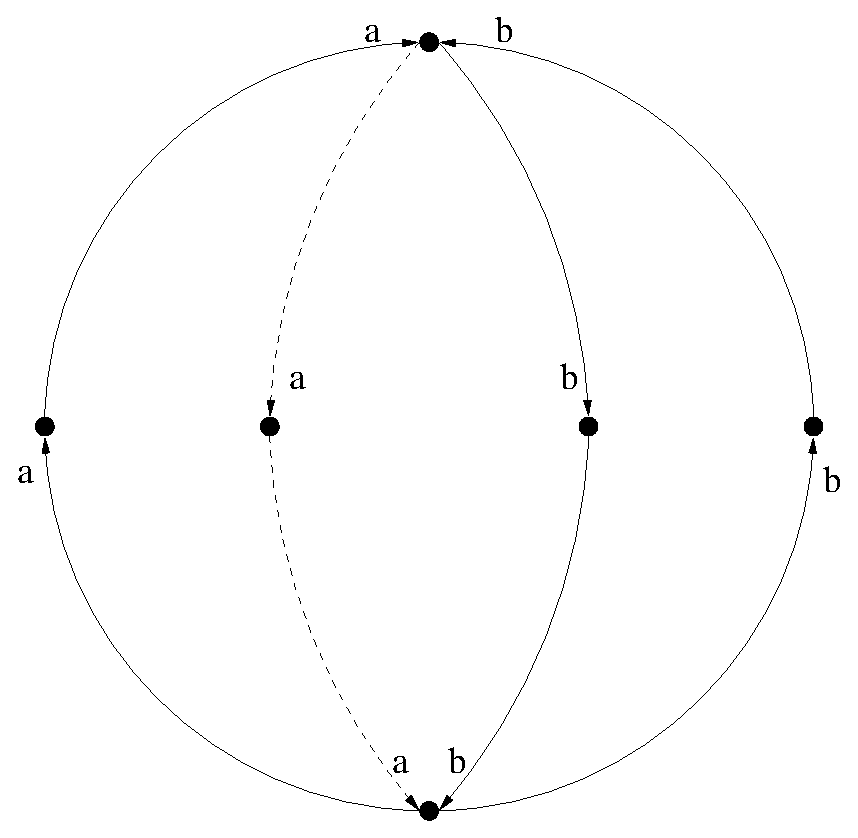
\includegraphics[scale = 0.75]{xmodcat1/q8-vankampen.eps}
%% \input{q8-vankampen.pstex_t} 
\end{center}

In the van Kampen diagrams, the four relators tile a sphere as shown above. 
Tracing out $\partial \iota$ we walk around the boundaries, 
with every edge cancelling out with its inverse. 


\newpage
%%%%%%%%%%%%%%%%%%%%%%%%%%%%%%%%%%%%%%%%%%%%%%%%%%%%%%%%%%%%%%%%%%%%%%%%
\subsection{A Geometric Example of Crossed Modules} \label{subs:geom-ex}

The major geometric example of a crossed module can be expressed
in two ways.
Let $(X,A,a)$ be a based pair of spaces, with  $a \in A \subseteq X$. 
\index{homotopy groups}
The \emph{second relative homotopy group} $\pi_2(X,A,a)$
consists of homotopy classes rel $J^1$ of continuous maps
$$
\alpha \;:\; (I^2, \dot{I}^2, J^1) \;\to\; (X,A,a)
$$
where  $I=[0,1]$  and  
$J^1=(\{0,1\} \times I) \cup (I \times \{1\}) \subset I^2$.
Each such  $\alpha$  is a map from the unit square  $I^2$  to the space  $X$ 
mapping the left, top, and right sides of the square to the point  $a$  
and the bottom side to a loop  $\beta_{\alpha}$ at  $a$.
We may represent such a map by the diagram in Figure 1.

\begin{figure}[htp] \label{fig:square}
\setlength{\unitlength}{1mm} 
\begin{center}
\begin{picture}(40,30)(0,5) 
\put(10,10){\vector(1,0){11}}
\put(21,10){\line(1,0){ 9}}
\put(10,30){\line(1,0){20}}
\put(10,10){\line(0,1){20}}
\put(30,10){\line(0,1){20}}
\put( 6,19){$a$}
\put(32,19){$a$}
\put(19,19){$\alpha$}
\put(19,31){$a$}
\put(19, 6){$\beta_{\alpha}$}
\end{picture} 
\caption{~An element  $\alpha \in \pi_2(X,A,a)$}
\end{center} 
\end{figure}

Recall that the fundamental group  $\pi_1(A,a)$  consists of maps  
$\gamma : I \to A, ~\gamma(0) = \gamma(1) = a$~.
With such a $\gamma$ it is easy to construct maps  $I^2 \to A$
which map two sides of the square to $a$ and two sides to $\gamma$:

\begin{figure}[!htp] \label{fig:squares}
\setlength{\unitlength}{1mm} 
\begin{center}
\begin{picture}(160,30)(0,5) 
\put(30,10){\vector(-1,0){11}}
\put(19,10){\line(-1,0){ 9}}
\put(30,30){\vector(-1,0){11}}
\put(19,30){\line(-1,0){ 9}}
\put(10,10){\line(0,1){20}}
\put(30,10){\line(0,1){20}}
\put(20,11){\line(0,1){2}}
\put(20,15){\line(0,1){2}}
\put(20,19){\line(0,1){2}}
\put(20,23){\line(0,1){2}}
\put(20,27){\line(0,1){2}}
\put(11,19){$a$}
\put(27,19){$a$}
\put(19,32){$\gamma$}
\put(19, 6){$\gamma$}

\put(60,10){\vector(-1,0){11}}
\put(49,10){\line(-1,0){ 9}}
\put(60,10){\vector(0,1){11}}
\put(60,21){\line(0,1){ 9}}
\put(40,10){\line(0,1){20}}
\put(40,30){\line(1,0){20}}
\put(50,11){\line(0,1){2}}
\put(50,15){\line(0,1){2}}
\put(50,19){\line(0,1){1}}
\put(50,20){\line(1,0){1}}
\put(53,20){\line(1,0){2}}
\put(57,20){\line(1,0){2}}
\put(41,19){$a$}
\put(49,31){$a$}
\put(61,19){$\gamma$}
\put(49, 6){$\gamma$}

\put(70,10){\vector(0,1){11}}
\put(70,21){\line(0,1){ 9}}
\put(90,10){\vector(0,1){11}}
\put(90,21){\line(0,1){ 9}}
\put(70,30){\line(1,0){20}}
\put(70,10){\line(1,0){20}}
\put(71,20){\line(1,0){2}}
\put(75,20){\line(1,0){2}}
\put(79,20){\line(1,0){2}}
\put(83,20){\line(1,0){2}}
\put(87,20){\line(1,0){2}}
\put(67,19){$\gamma$}
\put(91,19){$\gamma$}
\put(79,32){$a$}
\put(79, 6){$a$}

\put(100,10){\vector(1,0){11}}
\put(111,10){\line(1,0){ 9}}
\put(100,10){\vector(0,1){11}}
\put(100,21){\line(0,1){ 9}}
\put(120,10){\line(0,1){20}}
\put(100,30){\line(1,0){20}}
\put(110,11){\line(0,1){2}}
\put(110,15){\line(0,1){2}}
\put(110,19){\line(0,1){1}}
\put(110,20){\line(-1,0){1}}
\put(107,20){\line(-1,0){2}}
\put(103,20){\line(-1,0){2}}
\put(121,19){$a$}
\put(109,31){$a$}
\put( 97,19){$\gamma$}
\put(109, 6){$\gamma$}

\put(130,10){\vector(1,0){11}}
\put(141,10){\line(1,0){ 9}}
\put(130,30){\vector(1,0){11}}
\put(141,30){\line(1,0){ 9}}
\put(130,10){\line(0,1){20}}
\put(150,10){\line(0,1){20}}
\put(140,11){\line(0,1){2}}
\put(140,15){\line(0,1){2}}
\put(140,19){\line(0,1){2}}
\put(140,23){\line(0,1){2}}
\put(140,27){\line(0,1){2}}
\put(131,19){$a$}
\put(147,19){$a$}
\put(139,32){$\gamma$}
\put(139, 6){$\gamma$}

\end{picture} 
\caption{~Five maps $I^2 \to A$ derived from $\gamma \in \pi_1(A,a)$}
\end{center} 
\end{figure}

Whitehead showed in \cite{W-46} that there is a crossed module
$\Pi_2(X,A,a)$  with boundary map
% \begin{equation} \label{eq:topxm}
$$
\partial \;:\; \pi_2(X,A,a) \to \pi_1(A,a), \quad 
\alpha \mapsto \beta_{\alpha} = \alpha(I \times \{0\})~.
$$
% \end{equation}
The image of  $\alpha \in \pi_2(X,A,a)$
under the action of  $\gamma \in \pi_1(A,a)$ is illustrated in Figure 3, 
surounding $\alpha$ with the five maps in Figure 2.
Note that the boundary loop is the conjugate  
$\gamma^{-1}\beta_{\alpha}\gamma$.

\begin{figure}[!htp] \label{fig:action-diag}
\setlength{\unitlength}{1mm} 
\begin{center}
\begin{picture}(80,50)(0,5) 
\put( 10,10){\line(1,0){9}}
\put( 30,10){\vector(-1,0){11}}
\put( 30,10){\vector(1,0){11}}
\put( 41,10){\vector(1,0){20}}
\put( 70,10){\line(-1,0){9}}
\put( 10,30){\line(1,0){9}}
\put( 40,30){\vector(-1,0){21}}
\put( 40,30){\vector( 1,0){21}}
\put( 61,30){\line(1,0){9}}
\put( 10,50){\line(1,0){60}}

\put( 10,50){\line(0,-1){40}}
\put( 30,10){\vector(0,1){31}}
\put( 30,41){\line(0,1){9}}
\put( 50,10){\vector(0,1){31}}
\put( 50,41){\line(0,1){9}}
\put( 70,50){\line(0,-1){40}}

\put( 19,51){$a$}
\put( 39,51){$a$}
\put( 59,51){$a$}
\put(  7,39){$a$}
\put(  7,19){$a$}
\put( 71,39){$a$}
\put( 71,19){$a$}
\put( 27,19){$a$}
\put( 51,19){$a$}
\put( 39,31){$a$}
\put( 19, 6){$\gamma$}
\put( 39, 6){$\beta_{\alpha}$}
\put( 59, 6){$\gamma$}
\put( 19,26){$\gamma$}
\put( 59,26){$\gamma$}
\put( 31,39){$\gamma$}
\put( 46,39){$\gamma$}
\put( 39,19){$\alpha$}
\end{picture} 
\caption{Action of $\gamma$ on $\alpha$}
\end{center} 
\end{figure}

The meaning of this composite square is as follows.
Squares may be joined along an edge when the values agree on that edge.
If a composite is then $p$ units across by $q$ units high,
scaling factors $1/p$ horizontally and $1/q$ vertically are used
to obtain a new map from $I^2$ to $X$.


\begin{figure}[!htp] \label{fig:illustration}
\setlength{\unitlength}{1mm} 
\begin{center}
\begin{picture}(160,35)(-5,-2)
% left-hand square
\put( 10,10){\line(1,0){4}}
\put( 20,10){\vector(-1,0){6}}
\put( 20,10){\vector(1,0){6}}
\put( 26,10){\vector(1,0){10}}
\put( 36,10){\line(1,0){4}}
\put( 10,20){\line(1,0){30}}
\put( 10,30){\line(1,0){30}}

\put( 10,30){\line(0,-1){20}}
\put( 20,30){\line(0,-1){20}}
\put( 30,30){\line(0,-1){20}}
\put( 40,30){\line(0,-1){20}}

\put(  7,14){$a$}
\put( 41,14){$a$}
\put( 14, 6){$\beta_2$}
\put( 24, 6){$\beta_1$}
\put( 34, 6){$\beta_2$}
\put( 34,24){$a$}
\put( 24,24){$a$}
\put( 14,24){$a$}
\put( 12,14){$\alpha_2^{-1}$}
\put( 24,14){$\alpha_1$}
\put( 34,14){$\alpha_2$}

% middle square
\put( 60,10){\line(1,0){4}}
\put( 70,10){\vector(-1,0){6}}
\put( 70,10){\vector(1,0){6}}
\put( 76,10){\vector(1,0){10}}
\put( 86,10){\line(1,0){4}}
\put( 60,20){\line(1,0){4}}
\put( 75,20){\vector(-1,0){11}}
\put( 75,20){\vector( 1,0){11}}
\put( 86,20){\line(1,0){4}}
\put( 60,30){\line(1,0){30}}

\put( 60,30){\line(0,-1){20}}
\put( 70,30){\line(0,-1){20}}
\put( 80,30){\line(0,-1){20}}
\put( 90,30){\line(0,-1){20}}

\put( 64,31){$a$}
\put( 84,31){$a$}
\put( 57,24){$a$}
\put( 57,14){$a$}
\put( 91,24){$a$}
\put( 91,14){$a$}
\put( 64, 6){$\beta_2$}
\put( 74, 6){$\beta_1$}
\put( 84, 6){$\beta_2$}
\put( 64,16){$\beta_2$}
\put( 84,16){$\beta_2$}
\put( 74,24){$a$}
\put( 62,24){$\alpha_2^{-1}$}
\put( 74,14){$\alpha_1$}
\put( 84,24){$\alpha_2$}

% right-hand square
\put(110,10){\line(1,0){4}}
\put(120,10){\vector(-1,0){6}}
\put(120,10){\vector(1,0){9}}
\put(129,10){\vector(1,0){16}}
\put(142,10){\line(1,0){4}}
\put(110,20){\line(1,0){4}}
\put(125,20){\vector(-1,0){11}}
\put(125,20){\vector( 1,0){17}}
\put(142,20){\line(1,0){4}}
\put(110,30){\line(1,0){36}}

\put(110,30){\line(0,-1){20}}
\put(120,10){\vector(0,1){16}}
\put(120,30){\line(0,-1){4}}
\put(136,10){\vector(0,1){16}}
\put(136,30){\line(0,-1){4}}
\put(146,30){\line(0,-1){20}}

\put(114,31){$a$}
\put(127,31){$a$}
\put(140,31){$a$}
\put(107,24){$a$}
\put(107,14){$a$}
\put(147,24){$a$}
\put(147,14){$a$}
\put(114, 6){$\beta_2$}
\put(127, 6){$\beta_1$}
\put(140, 6){$\beta_2$}
\put(114,16){$\beta_2$}
\put(140,16){$\beta_2$}
\put(115,24){$\beta_2$}
\put(137,24){$\beta_2$}
\put(127,14){$\alpha_1$}
\put(123,24){$\alpha_2^{-1}\alpha_2$}

% extra bits
\put( 48,20){$\sim$}
\put( 98,20){$\sim$}
\put( 17,-2){$\alpha_2^{-1} \alpha_1 \alpha_2$}
\put(118,-2){${\alpha_1}^{\beta_2} \;=\; {\alpha_1}^{\partial\alpha_2}$}
\end{picture} 
\caption{~Verification of \textbf{X2:} for  $\Pi_2(X,A,a)$~.}
\end{center} 
\end{figure}

Figure 4 gives an outline verification of the second crossed module axiom
for $\Pi_2(X,A,a)$, where a square marked $a$ represents the constant 
map  $I^2 \to \{a\}$.

Whitehead's main result in \cite{W-41,W-46,W-49a} was:
\begin{thm} {\rm (Whitehead)} \label{thm:W} 
If  $X$  is obtained from  $A$  by attaching $2$-cells, 
then  $\pi_2(X,A,a)$  is isomorphic to the free crossed
$\pi_1(A,a)$-module on the attaching maps of the $2$-cells.
\end{thm}

\noindent
{\bf [More here?]}


%%%%%%%%%%%%%%%%%%%%%%%
% xmodcat1_10_10.tex  (30/04/07)

%%%%%%%%%%%%%%%%%%%%%%%%%%%%%%%%%%%%%%%%%%%%%%%%%
\subsection{Semidirect Products} \label{subs:sdp}

We include here some basic results on semidirect products
which will be needed in later sections.

\begin{prop}\quad\\
\vspace{-3mm}
\begin{enumerate}[{\rm (a)}]
\item
If a set  $X$  has a right  $G$-action  $x \mapsto x^g$
then $X$ has an associated left $G$-action:
$$
{}^g\!x \quad := \quad x^{g^{-1}}~.
$$
\item
The semidirect products  $R \ltimes S$  and  $S \rtimes R$
have multiplication rules
\begin{eqnarray*}
(r,s)(q,t)  & = &  (rq,\,s^q\,t) \quad\mbox{in}\quad R \ltimes S~, \\
(s,r)(t,q)  & = &  (s\,{}^r\!t,\,rq) \quad\mbox{in}\quad S \rtimes R~.
\end{eqnarray*}
\item
There is an isomorphism between these two groups:
$$
\psi \;:\; R \ltimes S \to S \rtimes R\,,
\quad (r,s) \mapsto (\,{}^r\!s,\,r)~,
$$
with inverse
$$
\psi^{-1} \;:\; S \rtimes R \to R \ltimes S\,,
\quad (s,r) \mapsto (r,\,s^r)~.
$$
\end{enumerate}
\end{prop}

%%%%%%%%%%%%%%%%%%%%%%%


%%%%%%%%%%%%%%%%%%%%%%%%%%%%%%%%%%%%%%%%%%%%%
\subsection{Cat1-groups} \label{subs:cat1} \index{cat$^1$-group} 

In \cite{loday1} Loday reformulated the notion of a 
crossed module as a cat$^1$-group $(G;t,h)$, 
namely a group $G$ with a pair of endomorphisms $t,h : G \to G$
having a common image $R$ and satisfying certain axioms. 
(We call these \emph{traditional} cat$^1$-groups.) 
Alternatively we may define a cat$^1$-group as follows. 

\begin{defn} \label{defn:cat1-group}
A \emph{cat$^1$-group} $\calC = (e;t,h : G \to R )$  
has source group $G$, range group $R$, and three homomorphisms:  
two surjections  $t,h : G \to R$ and an embedding  $e : R \to G$ 
as shown in the following diagram:
$$
\xymatrix{
 G  \ar[rr] <1.0ex>^{t,h} \ar[rr] <0.2ex>
   &&  R \ar[ll] <1.0ex>^e \\
}
$$

\noindent
These homomorphisms are required to satisfy the following axioms:
\begin{center}
\begin{tabular}{r l}
\textbf{C1:}  &  $(t \circ e)$ and $(h \circ e)$ 
are the identity mapping on $R$, \\
\textbf{C2:}  &  $[\ker t, \ker h] = \{ 1_G \}$.
\end{tabular}
\end{center}
\end{defn} 

The maps  $t,h$  are usually referred to as the 
\index{tail!of a cat$^1$-group} \index{head!of a cat$^1$-group} 
\index{embedding!of a cat$^1$-group} 
\emph{source} and \emph{target}, but we choose to call them the 
\emph{tail} and \emph{head} of  $\calC$, 
because \emph{source} is the {\GAP} term for the domain of a function. 
It follows immediately from axiom {\bf C1:} that: 
$$
t \circ e \circ t = t,\quad h \circ e \circ h = h,\quad 
t \circ e \circ h = h,\quad h \circ e \circ t = t.
$$

A morphism  $\calC_1 \to \calC_2$  \index{morphism!of cat$^1$-groups}
of cat$^1$-groups is a pair  $(\gamma, \rho)$  where
$\gamma : G_1 \to G_2$  and  $\rho : R_1 \to R_2$  
are homomorphisms satisfying
\begin{equation} \label{eq:cat1mor}
t_2 \circ\gamma = \rho\circ t_1, \quad
h_2 \circ\gamma = \rho\circ h_1, \quad
e_2 \circ\rho = \gamma\circ e_1.
\end{equation}

Of course a cat$^1$-group $(e;t,h : G \to R)$ is easily converted 
to a traditional cat$^1$-group $(G;t*e,h*e)$ and $(\id,e)$ 
is the cat$^1$-morphism between them. 

An arbitrary cat$^1$-group  $\calC = (e;t,h : G \to R)$
is isomorphic to the cat$^1$-group
$\calC' = (e';t',h' : R \ltimes S \to R)$
where  $S = \ker t$,  
the action of $R$ on $S$ is given by
$$
s^r = s^{er} = (er)^{-1} s (er),
$$
and the semidirect product  $R \ltimes S$  
has composition and inverse given by
$$
(r_1,s_1)(r_2,s_2) \; = \; (r_1r_2,{s_1}^{r_2}s_2), \;\;
(r,s)^{-1}  \; = \; (r^{-1}, (s^{-1})^{r^{-1}}).
$$
Since $R$ acts on both itself (by conjugation) and on $S$,
it also acts on $G$:
\begin{equation} \label{eq:RactsonG}
g^r ~=~ (er^{-1})g(er),  \quad\quad
(r_0,s_0)^r ~=~ (r^{-1}r_0r, s_0^r)\,.
\end{equation}

\noindent
The homomorphisms in  $\calC'$  are given by
\begin{equation} \label{eq:sdpcat1}
t'(r,s) = r, \quad h'(r,s) = r(\partial s), \quad e'r = (r,1).
\end{equation}

\begin{defn} \index{semidirect factorisation!for cat1-groups}
The \emph{semidirect factorisation} of $\calC$ is 
$(\phi, ~\id_R) : \calC \to \calC'$, where
\begin{equation} \label{eq:cat1-sdp-fact} 
\phi ~:~ G \to R \ltimes S, \quad g \mapsto (tg,ug),
\qquad\mbox{where}~~  ug = (etg^{-1})g. 
\end{equation}
The inverse isomorphism is  $(\phi^{-1}, ~\id_R) : \calC' \to \calC$, where 
$$
\phi^{-1} ~:~ R \ltimes S \to G, \quad (r,s) \mapsto (er)s.
$$ 
\end{defn}

\begin{lem} \label{lem:u-props}
The mapping $u : G \to \ker t,\; g \mapsto (etg^{-1})g$ has the
following properties.
\begin{enumerate}[{\rm (i)}]
\item~ $u^2 = u,$
\item~ $tug = 1_R,\quad hug = (tg^{-1})(hg),\quad uer = 1_G, $
\item~ $u(g_1g_2) = (ug_2)(ug_1)^{g_2},$
\item~ $(ug)^{-1} = g^{-1}(etg) = (u(g^{-1}))^g.$
\end{enumerate}
\end{lem}
The crossed module $\calX = (\partial : S \to R)$  
associated to  $\calC$  and  $\calC'$  has boundary 
$\partial = h\hspace{-5pt}\mid_S$ and action $s^r := s^{er}$. 
The cat$^1$-group  $\calC = \calC'$  associated to  
$\calX = (\partial : S \to R)$  has  $G = R \ltimes S$, 
where the action is that in  $\calX$,
and homomorphisms given by (\ref{eq:sdpcat1}).
We denote by  $\epsilon$  the inclusion of  $S$  in  $G$,
so that  $\partial = h \epsilon$.

Given a morphism 
$(\sigma,\rho) : \calX_1 \to \calX_2$ of crossed modules,
the associated morphism of cat1-groups is
$(\gamma,\rho) : \calC_1 \to \calC_2$ where
$\gamma(r_1,s_1) = (\rho r_1, \sigma s_1)$.
Similarly, given a morphism 
$(\gamma,\rho) : \calC_1 \to \calC_2$ of cat1-groups,
the associated morphism of crossed modules is
$(\sigma,\rho) : \calX_1 \to \calX_2$ where
$\sigma s = \gamma(1,s)$.


George Janelidze has noted the following variant of the second
cat$^1$-group axiom:
$$
\textbf{C2}'\textbf{:}  \qquad  
%%% [~(etg_1^{-1})\,g_1,\, (ehg_2^{-1})\,g_2~] ~=~ 1_G
[ug_1,ug_2] ~=~ 1_G
\qquad \text{for all}~~ g_1,g_2 \in G~.
$$
It follows that cat$^1$-groups form an equational variety.

\begin{lem}
If  $\calC = (e;t,h : G \to R )$  is a cat$^1$-group
then there is a group homomorphism
$$
(t,h) ~:~ G \to R \times R, ~ g \mapsto (tg,hg)~.
$$
\end{lem}


\begin{prop}
\emph{(Comment by Tim Porter during a seminar on 18/10/02.)\\}
A \emph{congruence}  $\equiv$ 
(in the sense of congruence on a monoid) 
on a group $R$ gives rise to a cat$^1$-group.
\end{prop}
\begin{pf}
The set of equivalent pairs,
$$
G ~=~ \{(r_1,r_2) \in R \times R ~~|~~ r_1 \equiv r_2 \}
$$
is a subgroup of  $R \times R$.
The required  $\calC = (e;t,h : G \to R )$  has homomorphisms given by:
$$
t(r_1,r_2) = r_1, \qquad
h(r_1,r_2) = r_2, \qquad
e(r) = (r,r).
$$
The associated crossed module has source
$$
\ker t ~=~ \{(r,1) ~|~ r \equiv 1 \}
$$
which shows that the elements equivalent to $1_R$ in the congruence
form a normal subgroup.
\end{pf}



%%%%%%%%%%%%%%%%%%%%%%%%%%%%%%%%%%%%%%%%%%%%%%%%%%%%%%%%%%%%%%%%%%%%%
\subsection{Pre-cat$^1$-groups} \index{pre-cat$^1$-groups} 

When axioms \textbf{X2:} and \textbf{C2:} are \emph{not} satisfied
by  $\calQ = (\delta : Q \to R)$  and  
$\calB = (e;t,h : R \ltimes Q \to R)$,
the corresponding structures are known as \emph{pre-crossed modules}
and \emph{pre-cat$^1$-groups}.
In this case recall from Subsection \ref{subs:Peiffer}
that the \emph{Peiffer subgroup}  $P$  of  $Q$  is the subgroup of
$\ker(\delta)$  generated by \emph{Peiffer commutators}
$$
\langle q_1, q_2 \rangle 
\;=\; 
q_1^{-1}\,q_2^{-1}\,q_1\,{q_2}^{\partial q_1}~.
$$
Then  $\calP = (0 : P \to \{1_R\})$  
is a normal sub-pre-crossed module of  $\calQ$  and  
$\calX = \calQ/\calP = (\partial : S=Q/P \to R)$  is a crossed module.
The restriction of  $\epsilon : Q \to R \ltimes Q$  to  $P$  is given by
$$
   \epsilon \langle q_1, q_2 \rangle
 = [ (\delta q_1^{-1}, q_1), (1_R, {q_2}^{\delta q_1}) ]
 \in  [ \ker h, \ker t ].
$$
The image  $\epsilon P$  is the Peiffer subgroup
$[\ker h, \ker t]$  of  $R \ltimes Q$
and, if  $\iota$  is the inclusion  $\{ 1_R \} \to R$,  then
$\calC/(\epsilon,\iota)\calP = 
 (e;t,h : (R \ltimes Q) / \epsilon P \to R)$
is the cat$^1$-group corresponding to  $\calX = \calQ/\calP$.


%%%%%%%%%%%%%%%%%%%%%%%%%%%%%%%%%%%%%%%%%%%%%%%
\subsection{Sub-cat$^1$-groups} \label{subs:sub-cat1} 

We need to include here clear definitions of sub-cat$^1$-groups 
and normal sub-cat$^1$-groups. 
Also the kernel of a cat$^1$-morphism. 



%%%%%%%%%%%%%%%%%%%%%%%%%%%%%%%%%%%%%%%%%%%%%%%
\subsection{Group Groupoids} \label{subs:gpgpd} \index{group-groupoid} 

Cat1-groups may also be thought of as group-groupoids.
A group groupoid is a set which has both a group structure and
a groupoid structure (see subsection \ref{subsect:gpds}). 
From a categorical viewpoint, it is both a group object in the
category of groupoids and a groupoid object in the category of groups.

The underlying groupoid $\calG$  of a cat$^1$-group  $\calC$ 
\index{underlying groupoid!of a cat$^1$-group} 
has the group $R$ as object set $G_0$ 
and the group $G$ as the set of arrows $G_1$. 
The identity arrow at  $r$  is  $1_r = er$. 
For each arrow  $g$  the tail (source) is  $tg$ and the head (target) is $hg$. 
Arrows  $g_1,g_2$  are composable only when  $hg_1 = tg_2 = r_1$ (say),
in which case the composite arrow is
\begin{equation} \label{eq:gpgpd-comp}
g_1 * g_2 ~=~ g_1(e{r_1}^{-1})g_2 
\quad\mbox{where}\quad
t(g_1 * g_2) = tg_1 = r_0, \quad
h(g_1 * g_2) = hg_2 = r_2.
\end{equation}

\noindent
This composition is, of course, associative:
$$
g_1*g_2*g_3 ~=~ g_1({er_1}^{-1})g_2({er_2}^{-1})g_3.
$$

\noindent
The groupoid inverse  $\tilde{g}$  of  $g$  for the composition is given by
$$
\tilde{g} \; = \; (ehg)g^{-1}(etg)
\quad \mbox{with} \quad  
t \tilde{g} = hg, \; h \tilde{g} = tg, \; g * \tilde{g} = etg  
\;\; \mbox{and} \;\;
\tilde{g} * g = ehg~.
$$  

$$
\xy
\xymatrix{
  &&&&&&&& \\
  &  r_0=tg_1 \ar `u[-1,-1] `[1,-1] `[1,0]_{er_0} `[0,0] [0,0]
            \ar@/^3ex/[rrr]^{g_1}
            \ar `u[-1,1] `[0,6]^{g_1 * g_2} [0,6]
  &&& hg_1=r_1=tg_2 \ar@/^3ex/[rrr]^{g_2}
                    \ar@/^3ex/[lll]^{\tilde{g}_1}
                    \ar@(ur,ul)_{er_1}
     &&& r_2=hg_2 \ar `d[1,1] `[-1,1] `[-1,0]_{er_2} `[0,0] [0,0]
                  \ar@/^3ex/[lll]^{\tilde{g}_2}
                  \ar `d[1,-1] `[0,-6]^{\widetilde{g_1 * g_2}} [0,-6] 
         & \\
  &&&&&&&& \\
}
\endxy
$$

\noindent
Hence the composites of one element with the groupoid inverse of another, 
when defined, are given by 
\begin{equation} \label{eq:inv-comps}
\tilde{g}_1 * g_3 ~=~ (ehg_1)g_1^{-1}g_3
\qquad\mbox{and}\qquad
g_4 * \tilde{g}_2 ~=~ g_4g_2^{-1}(etg_2).
\end{equation}

\medskip\noindent
The equivalent formulae for composition and inverse 
when  $R \ltimes S$  replaces $G$ are:
$$
(r, s) * (r (\partial s), s') = (r, ss')
\quad \mbox{and} \quad  
\widetilde{(r,s)} = (r(\partial s), s^{-1})~.
$$

Since  $g^{-1}(etg) \in \ker t$  and  $(ehg)g^{-1} \in \ker h$,
the map  $g \mapsto \tilde{g}$  is an automorphism of  $\calG$
which restricts to the identity map on  $eR$  and
provides a cat$^1$-isomorphism from  $\calC$  to the \emph{reverse}
cat$^1$-group $\tilde{\calC} = (e;h,t : G \to R)$ of $\calC$.
The set of arrows \emph{out} from  $1_R$  is  $\ker t$
while the set of arrows \emph{in} to  $1_R$  is  $\ker h$,
so  $\ker \partial$  is the set of loops at  $1_R$.
The set of objects in the component of  $\calG$
connected to  $1_R$  is the image of  $\partial$,
so  $\calG$  is discrete when  $\partial = 0$.

Alternatively, starting with a group groupoid $\calG = (G,t,h)$, define
\begin{eqnarray*}
  R & = & \im t ~=~ \im h, \\
  S & = & \{g ~|~ tg = 1\} ~=~ \ker t ~=~ \mbox{arrows out from}~ 1_R, \\
s^r & = & (er)^{-1}s(er), 
\quad\text{where}~ er ~\text{is the identity loop at}~ r.
\end{eqnarray*}

\bigskip\noindent
See Subsection \ref{subs:gpd-sect} for the group-groupoid 
equivalent of derivations and sections.


\bigskip
\begin{example}
\emph{The normal inclusion crossed module $X_3 = (1 : C_3 \to S_3)$ 
of the cyclic group $C_3 = \langle c ~|~ c^3 \rangle$ 
in the symmetric group $S_3 = \langle a,b ~|~ a^3, b^2, (ab)^2 \rangle$,
with conjugation action $c^a=c, c^b=c^2$,
has associated cat$^1$-group $(e;t,h : S_3 \ltimes C_3 \to S_3)$.
The images of the tail and head functions are given in the following table:}
\begin{center}
\begin{tabular}{|ccc|ccc|}
\hline
$g$ & $tg$ & $hg$ & $g$ & $tg$ & $hg$ \\
\hline
$(1,1)$ & $1$ & $1$ &        $(b,1)$ & $b$ & $b$ \\
$(1,c)$ & $1$ & $a$ &        $(b,c)$ & $b$ & $ba$ \\
$(1,c^2)$ & $1$ & $a^2$ &    $(b,c^2)$ & $b$ & $ab$ \\
$(a,1)$ & $a$ & $a$ &        $(ab,1)$ & $ab$ & $ab$ \\
$(a,c)$ & $a$ & $a^2$ &      $(ab,c)$ & $ab$ & $b$ \\
$(a,c^2)$ & $a$ & $1$ &      $(ab,c^2)$ & $ab$ & $ba$ \\
$(a^2,1)$ & $a^2$ & $a^2$ &  $(ba,1)$ & $ba$ & $ba$ \\
$(a^2,c)$ & $a^2$ & $1$ &    $(ba,c)$ & $ba$ & $ab$ \\
$(a^2,c^2)$ & $a^2$ & $a$ &  $(ba,c^2)$ & $ba$ & $b$ \\
\hline
\end{tabular}
\end{center}
\emph{The corresponding group-groupoid has $6$ objects, $18$ morphisms, 
$2$ connected components, and may be pictured as:}
\begin{center}
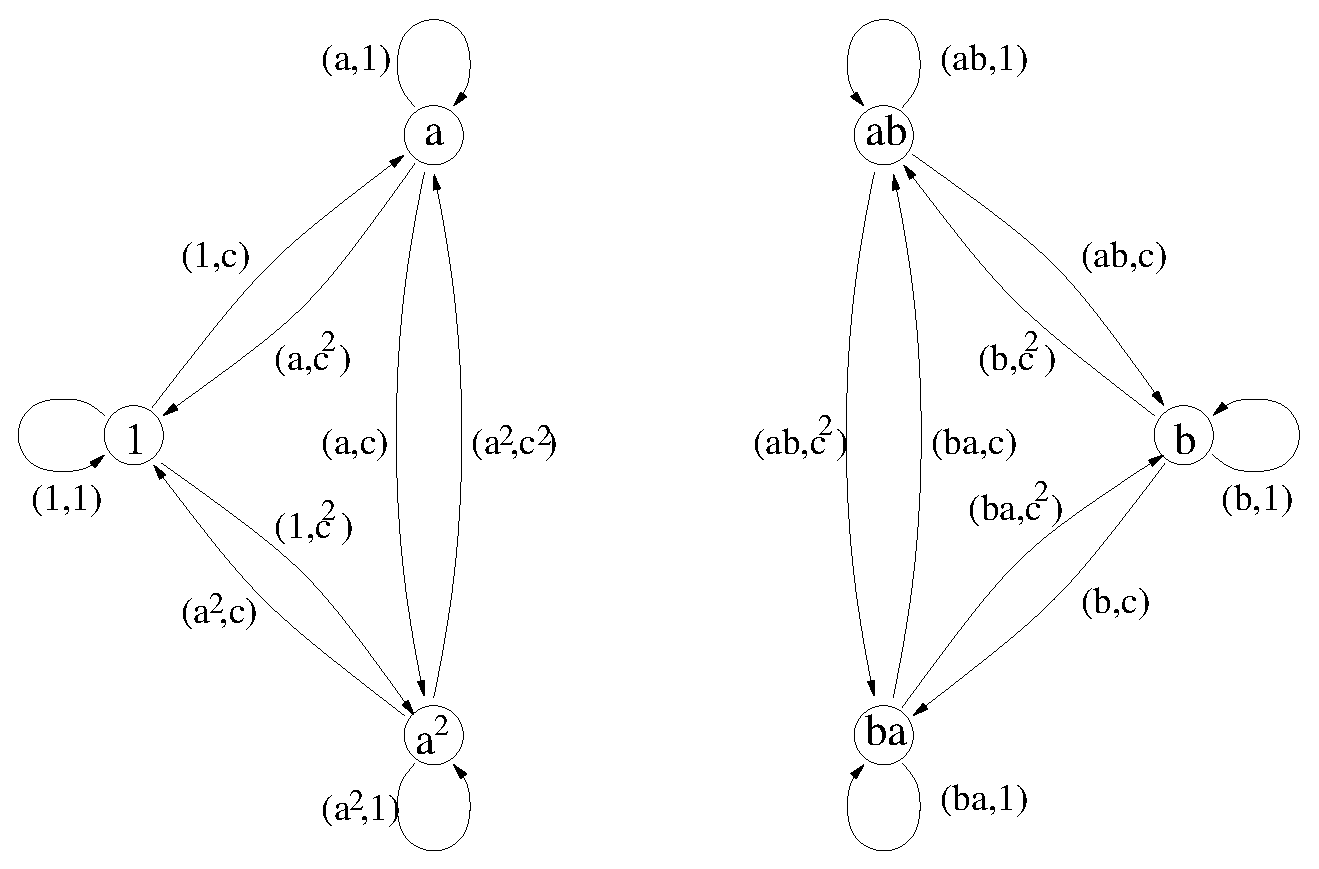
\includegraphics[scale = 0.65]{xmodcat1/s3ggpd.eps}
%% \input{s3ggpd.pstex_t} 
\end{center}

\noindent
\emph{We may compare the group multiplication with the groupoid multiplication
by calculating, for example,}
\begin{eqnarray*}
(a,c)(a^2,c) &=& (1,c^{a^2}c) ~=~ (1,c^2), \\
(a,c)*(a^2,c)     &=& (a,c)(a^2,1)^{-1}(a^2,c) ~=~ (a^4,c^{a^3}c) ~=~ (a,c^2).
\end{eqnarray*}
\end{example}





\newpage
%%%%%%%%%%%%%%%%%%%%%%%%%%%%%%%%%%%%%%%%%%%
\subsection{$2$-groups} \label{subs:twogps}

Finally, we think of such a structure as a special case of a 
\index{$2$-category} \index{$2$-group} \index{$2$-cell} 
$2$-category, which has objects, morphisms, and $2$-\emph{cells}.
We follow the presentation in Subsection 1.2.3 of 
Forrester-Barker's thesis \cite{f-b-thesis}. 
For an introduction to $2$-groupoids, 
see Kamps and Porter \cite{kamps:port}.
Note that a $2$-group is \emph{not} a special case of the group theorist's 
$p$-group, with $p=2$, but is a $2$-category with one object having all 
morphisms and $2$-cells invertible.

The $2$-group $\calH$ associated to $\calX = (\partial : S \to R)$ has
\begin{itemize}
\item  a single object $\bullet$,
\item  morphisms $r \in R$,
\item  $2$-cells $(r,s) \in R \ltimes S$
       with tail $r$ and head $r(\partial s)$.
\end{itemize}
$$
\xy
\xymatrix{
   & & & \\
 \Downarrow (r,s)~= 
   & \bullet  \ar@/^5ex/[rr]^{r} 
              \ar@/_5ex/[rr]_{r(\partial s)} 
     & \Downarrow (r,s)
        & \bullet \\
   & & & \\
}
\endxy
$$

%\medskip
\noindent
Horizontal composition $(r_1,s_1) \sharpz (r_2,s_2)$ 
of $2$-cells is given by
$$
\xy
\xymatrix{
  & &  & & & & & & \\
  \bullet \ar@/^5ex/[rr]^{r_1} 
          \ar@/_5ex/[rr]_{r_1(\partial s_1)} 
  & \Downarrow (r_1,s_1)
    & \bullet \ar@/^5ex/[rr]^{r_2} 
              \ar@/_5ex/[rr]_{r_2(\partial s_2)} 
      & \Downarrow (r_2,s_2)
        & \bullet 
          & = 
            & \bullet \ar@/^5ex/[rr]^{r_1r_2} 
                      \ar@/_5ex/[rr]_{r_1(\partial s_1)r_2(\partial s_2)} 
              & \Downarrow (r_1r_2,{s_1}^{r_2}{s_2})
                & \bullet \\
  & & & & & & & & \\
}
\endxy
$$

%\medskip
\noindent
There is a unique \emph{horizontal identity} $2$-cell
$$
\xy
\xymatrix{
   & & & \\
 \Downarrow(1,1)~=
   & \bullet  \ar@/^5ex/[rr]^{1} 
             \ar@/_5ex/[rr]_{1} 
     & \Downarrow (1,1)
        & \bullet \\
   & & & \\
}
\endxy
$$

%\medskip
\noindent
Similarly, when $r_1(\partial s_1) = r_3$,
vertical composition $(r_1,s_1) \sharpo (r_3,s_3)$ 
of $2$-cells is given by
$$
\xy
\xymatrix{
  && && & & && \\
  && \Downarrow (r_1,s_1)
     && & & && \\
  \bullet \ar@/^15ex/[rrrr]^{r_1} 
          \ar[rrrr]^{r_1(\partial s_1)}
          \ar@/_15ex/[rrrr]_{r_1(\partial s_1)(\partial s_3)} 
  && && \bullet 
        &=& \bullet \ar@/^5ex/[rr]^{r_1} 
                    \ar@/_5ex/[rr]_{r_1(\partial(s_1s_3))} 
            & \Downarrow (r_1,s_1s_3)
             & \bullet \\
  && \Downarrow (r_1(\partial s_1),s_3)
     && & & && \\
  && && & & && \\
}
\endxy
$$

\medskip\noindent
For each $r \in R$ there is a \emph{vertical identity} $2$-cell 
$$
\xy
\xymatrix{
   & & & \\
 \Downarrow(r,1)~=
   & \bullet  \ar@/^5ex/[rr]^{r} 
             \ar@/_5ex/[rr]_{r} 
     & \Downarrow (r,1)
        & \bullet \\
   & & & \\
}
\endxy
$$
such that
$$
\Downarrow(r,1)\; \sharpo \Downarrow(r,s)\; 
                  \sharpo \Downarrow(r(\partial s),1)
~=~ \Downarrow(r,s).
$$

The \emph{horizontal inverse} and the 
\emph{vertical right inverse} of $\Downarrow(r,s)$ 
are $\Downarrow(r^{-1},(s^{-1})^{r^{-1}})$ 
and $\Downarrow(r(\partial s),s^{-1})$ respectively.

Horizontal composition with vertical identities is called 
\emph{whiskering}. 
In diagrams it is often convenient to shrink $\Downarrow(q,1)$ 
to a single arc, labelled $q$, as in the whiskering formlae:
$$
q_1 \sharpz \Downarrow(r,s) ~\sharpz~ q_2 
~=~ \Downarrow(q_1rq_2,{s}^{q_2}).
$$

\bigskip\noindent
The Peiffer condition for cat$^1$-groups establishes an 
\index{Peiffer condition} \index{interchange law} 
\emph{interchange law} for $\calH$,
$$
((r_1,s_1) \sharpz (r_2,s_2)) \sharpo ((r_3,s_3) \sharpz (r_4,s_4))
\quad = \quad
((r_1,s_1) \sharpo (r_3,s_3)) \sharpz ((r_2,s_2) \sharpo (r_4,s_4)) 
$$
for the well-defined composite 
when $r_1(\partial s_1) = r_3$ and $r_2(\partial s_2) = r_4$,
$$
\xy
\xymatrix{
  && && && && \\
  && \Downarrow (r_1,s_1)
     && && \Downarrow (r_2,s_2)
           && \\
  \bullet \ar@/^15ex/[rrrr]^{r_1} 
          \ar[rrrr]^{r_1(\partial s_1) = r_3}
          \ar@/_15ex/[rrrr]_{r_3(\partial s_3)} 
  && && \bullet \ar@/^15ex/[rrrr]^{r_2} 
                \ar[rrrr]^{r_2(\partial s_2) = r_4}
                \ar@/_15ex/[rrrr]_{r_4(\partial s_4)} 
        && && \bullet \\
  && \Downarrow (r_3,s_3)
     && && \Downarrow (r_4,s_4)
           && \\
  && && && && \\
}
\endxy
$$

\noindent
When this composite is defined, 
$$
    s_2{s_3}^{r_4}
~=~ s_2{s_3}^{r_2(\partial s_2)}
~=~ {s_3}^{r_2}s_2
$$
and the composite $2$-cell is
$$
\xy
\xymatrix{
   && && \\
   \bullet \ar@/^5ex/[rrrr]^{r_1r_2} 
           \ar@/_5ex/[rrrr]_{r_3(\partial s_3)r_4(\partial s_4)} 
   && \Downarrow (r_1r_2,(s_1s_3)^{r_2}s_2s_4)
      && \bullet \\
   && && \\
}
\endxy
$$



%% derivations and sections 
\newpage % der-sect.tex  (02/05/17)

%%%%%%%%%%%%%%%%%%%%%%%%%%%%%%%%%%%%%%%%%%%%%%%%%%%%%%%
\section{Derivations and Sections} \label{sect:der-sec}


%%%%%%%%%%%%%%%%%%%%%%%%%%%%%%%%%%%%%%%%%%%%%%%%%%%%%%%%%%%%%%%
\subsection{Derivations} \label{subsec:der} \index{derivations}

The Whitehead monoid \index{Whitehead monoid} $\Der(\calX)$  of  $\calX$ 
was defined in \cite{W-48b} 
to be the monoid of all {\it derivations}
from $R$ to $S$, that is the set of all maps  $R \to S$,
with composition  $\ \star \ $, satisfying
\begin{center}
\begin{tabular}{c r c l }
\textbf{D1:}  &  $\chi(qr)$              &  = 
           & $(\chi q)^{r} \; (\chi r)$  \\
\textbf{D2:}  &  $(\chi_1 \star \chi_2)(r)$  &  =
           & $(\chi_2 r)(\chi_1 r)(\chi_2 \partial \chi_1 r)$. 
\end{tabular}
\end{center}

\noindent
The definition of Whitehead multiplication used here 
differs from that in \cite{alp:wens-ijac} in that it is now 
defined as multiplication on the right rather than on the left, 
which is why we are using `$\star$' in place of `$\circ$'. 
Invertible elements in the monoid are called \emph{regular}. 
\index{regular derivation} \index{derivation!regular} 
The Whitehead group $W = W(\calX)$ is the group of the monoid. 

In Brown and Gilbert \cite{brow:gilb} the notion of derivation 
was extended to that of $\gamma$-derivation, as in the following definition. 
Since ordinary derivations may be obtained from $\gamma$-derivations 
by setting $\gamma$ to be the identity automorphism oh $\calX$, 
we shall give properties in terms of the more general case. 

\begin{defn} \index{$\gamma$-derivation}
If $\gamma = (\ddg,\dg)$ is an automorphism of $\calX$,
the Whitehead monoid $\Der_{\gamma}(\calX)$  of  $\calX$ 
is the monoid of all $gamma$-{\it derivations}
from $R$ to $S$, that is the set of all maps  $R \to S$,
with composition written  $\ \star_{\gamma} \ $, satisfying
\begin{center}
\begin{tabular}{c r c l }
\textbf{\emph{D1:}}  &  $\chi(qr)$              &  = 
           & $(\chi q)^{\dg r}(\chi r)~.$  \\
\textbf{\emph{D2:}}  &  $(\chi_1 \star_{\gamma} \chi_2)(r)$  &  =
           & $(\chi_2 r)(\chi_1 r)(\chi_2 \dg^{-1} \partial \chi_1 r)$. 
\end{tabular}
\end{center}
\end{defn}

The following Lemma verifies that $\Der_{\gamma}(\calX)$ \emph{is} a monoid.
 
\begin{lem} \label{lem:invchir}
\mbox{  }\\
\vspace{-5mm}
\begin{enumerate}[{\rm (a)}]
\item~
$\chi 1 = 1$~,
\item~
$(\chi r)^{-1} \;\;=\;\; (\chi\,r^{-1})^{\dg r}$~,
\item~
the zero map is a derivation and an identity for the Whitehead multiplication,
\item~
the Whitehead multiplication is associative. 
\end{enumerate}
\end{lem}
\begin{pf}
%\vspace{-5mm}
\begin{enumerate}[(a)]
\item
This follows from $\chi(r1) = (\chi r)^1(\chi 1)$.
\item 
This follows from  $1 = \chi(r^{-1}r) = (\chi r^{-1})^{\dg r}(\chi r)$~.
\item
It is clear that $0 : R \to S,~ r \mapsto 1$ is a derivation, and that
$$
(\chi\star_{\gamma}0)r = 1(\chi r)1 = \chi r = (\chi r)11 
= (0\star_{\gamma}\chi)r~.
$$
\item
Expansion by {\bf D2:} using either bracketing 
(though one requires more work!) gives: 
$$
(\chi_1 \star \chi_2 \star \chi_3)r \;\;=\;\;
(\chi_3 r)(\chi_2 r)(\chi_3\dg^{-1}\partial\chi_2 r)
(\chi_1 r)(\chi_3\dg^{-1}\partial\chi_1 r)(\chi_2\dg^{-1}\partial\chi_1 r)
(\chi_3\dg^{-1}\partial\chi_2\dg^{-1}\partial\chi_1 r)~.
$$
\end{enumerate}
\end{pf}

For $\chi$ a $\gamma$-derivation, define 
$\psi=\psi_{\chi} : R \to S$ by $\psi r = \chi \dg^{-1}r$ or, equivalently, 
$\psi\dg r = \chi r$.
\begin{equation} \label{eq:chi-psi}
\vcenter{\xymatrix{
   S \ar[rr]^{\ddg} \ar[dd]_{\partial} 
     && S \ar[dd] <0.5ex>^{\partial} \\
     &&  \\
   R \ar[uurr]^{\chi} \ar[rr]_{\dg} 
     && R \ar[uu] <0.5ex>^{\psi}
}}
\end{equation}

\noindent
Then $\psi$ is a (identity-) derivation since 
$$
\psi(qr)
~=~ \chi((\dg^{-1}q)(\dg^{-1}r)) 
~=~ (\chi\dg^{-1}q)^{\dg(\dg^{-1}r)}(\chi\dg^{-1}r) 
~=~ (\psi q)^r(\psi r).
$$

\begin{lem} \label{lem:wgamma-to-w} 
The map $\Der_{\gamma}(\calX) \to \Der(\calX),~ \chi \mapsto \psi_{\chi}$, 
is a monoid homomorphism. 
\end{lem} 
\begin{pf} 
If $\psi_1,\psi_2$ are the derivations corresponding to $\gamma$-derivations 
$\chi_1,\chi_2$, then 
\begin{eqnarray*}
(\psi_1 \star \psi_2)(\dg r)
  &=& (\psi_2\dg r)(\psi_1\dg r)(\psi_2\dg\dg^{-1}\partial\psi_1\dg r) \\
  &=& (\chi_2 r)(\chi_1 r)(\chi_2\dg^{-1}\partial\chi_1 r) \\
  &=& (\chi_1 \star_{\gamma} \chi_2)r.
\end{eqnarray*}
\end{pf} 


\begin{lem} \label{lem:gamma-beta-chi}
Given a $\gamma$-derivation $\chi$ of $\calX$ there is an endomorphism 
$\beta_{\chi} = (\ddb_{\chi}, \db_{\chi})$
of $\calX$ where
$$
\ddb_{\chi} : S \to S, \;\; s \mapsto (\ddg s)(\chi \partial s), \quad
 \db_{\chi} : R \to R, \;\; r \mapsto  (\dg r)(\partial \chi r)
$$
such that 
\begin{enumerate}[{\rm (a)}]
\item~
$\ddb_{\chi}(s^r) 
  \;\;=\;\;  (\ddb_{\chi}s)^{\db_{\chi}r}
  \;\;=\;\;  (\chi r)^{-1}\,(\ddb_{\chi} s)^{\dg r}\,(\chi r)$~,
\item~
$\db_{\chi}(q^r)
  \;\;=\;\;  (\db_{\chi}q)^{\db_{\chi}r}
  \;\;=\;\;  ((\dg r)(\partial\chi r))^{-1}(\dg q)(\partial\chi q)
                     ((\dg r)(\partial\chi r))$~, 
\item~ 
$(\chi_1\star_{\gamma}\chi_2) r 
\;=\;
(\chi_2 r)(\ddb_{\chi_2} \ddg^{-1} \chi_1 r)
\;=\;
(\chi_1 r)(\chi_2 \dg^{-1} \db_{\chi_1} r)$~,
\item~
$\chi\,*\,{\ddg}^{-1}\,*\,\ddb_{\chi}\ 
 \;=\; \db_{\chi}\,*\,{\dg}^{-1}\,*\,\chi
 \;:\; R \to S, \quad r \mapsto (\chi r)(\chi\dg^{-1}\partial\chi r)$\,,~
\emph{so that the following diagram commutes:}
\begin{equation} \label{eq:gamma-sqchi}
\vcenter{\xymatrix{
   S \ar[rrr]^{{\ddg}^{-1}\,*\,\ddb_{\chi}}
     &&& S \\
     &&&  \\
   R \ar[uu]^{\chi} \ar[rrr]_{\db_{\chi}\,*\,{\dg}^{-1}} 
     &&& R \ar[uu]_{\chi}
}}
\end{equation}
\item~
The endomorphism  $\ddb_{\chi} * \ddg^{-1}$  
commutes with  $\partial * \chi * \ddg^{-1}$  
while  $\dg^{-1} * \db_\chi$ commutes with  $\dg^{-1} * \chi * \partial$~. 
\item~
When $\psi = \psi_{\chi}$ as in \emph{(\ref{eq:chi-psi})}, 
then ~$\db_{\chi}r ~=~ \db_{\psi}(\dg r)$~ 
and ~$\ddb_{\chi}s ~=~ \ddb_{\psi}(\ddg s)$. 
\end{enumerate}
\end{lem}
\begin{pf}
We first check that $\db_{\chi}$ and $\ddb_{\chi}$ are homomorphisms.
\begin{eqnarray*}
\db_{\chi}(r_1r_2) 
  &=&   \dg(r_1r_2)\partial((\chi r_1)^{\dg r_2}(\chi r_2)) 
    ~=~ (\dg r_1)(\partial\chi r_1)(\dg r_2)(\partial\chi r_2) 
    ~=~ (\db_{\chi}r_1)(\db_{\chi}r_2), \\
\ddb_{\chi}(s_1s_2)
  &=&   \ddg(s_1s_2)(\chi((\partial s_1)(\partial s_2)) 
    ~=~ (\ddg s_1)(\ddg s_2)(\chi\partial s_1)^{\partial\ddg s_2}
           (\chi\partial s_2) 
    ~=~ (\ddb s_1)(\ddb s_2).
\end{eqnarray*}

\noindent
We now verify the six properties.
\begin{enumerate}[(a)]
\item
\mbox{}\vspace*{-9mm} 
\begin{eqnarray*} 
\ddb_{\chi}(s^r) 
  & = &  (\ddg s^r)(\chi\partial(s^r)) 
    \;=\; (\ddg s)^{\dg r}(\chi(r^{-1}(\partial s)r)) 
    \;=\; (\ddg s)^{\dg r}(\chi(r^{-1}))^{(\partial\ddg s)(\dg r)}
              (\chi\partial s)^{\dg r}(\chi r) \\
  & = &  \{(\chi(r^{-1}))(\ddg s)(\chi\partial s)\}^{\dg r}(\chi r) 
    \;=\;  (\chi r)^{-1}(\ddb_{\chi} s)^{\dg r}(\chi r) 
    \;=\;  (\ddb_{\chi} s)^{(\dg r)(\partial\chi r)} 
    \;=\;  (\ddb_{\chi} s)^{\db_{\chi}r}~.
\end{eqnarray*}
\item
\mbox{}\vspace*{-9mm} 
\begin{eqnarray*}
\db_{\chi}(q^r)
  & = &  (\dg(q^r))(\partial\chi(r^{-1}qr)) 
    \;=\;  (\dg(q^r))\,\partial\{(\chi(r^{-1}))^{\dg(qr)}
                (\chi q)^{\dg r}(\chi r)\} \\
  & = &  (\dg(q^r))(\partial\chi(r^{-1}))^{(\dg r)(\dg q^r)} 
                (\partial\chi q)^{\dg r}(\partial\chi r) 
    \;=\;  (\partial((\chi r)^{-1})(\dg(q^r))
                (\partial\chi q)^{\dg r}(\partial\chi r) \\
  & = &  (\partial\chi r)^{-1}\{(\dg q)(\partial\chi q)\}^{\dg r} 
                (\partial\chi r) 
    \;=\;  (\db_{\chi}q)^{\db_{\chi}r}~.
\end{eqnarray*}
\item 
\mbox{}\vspace*{-9mm} 
\begin{eqnarray*} 
(\chi_1\star_{\gamma}\chi_2)r 
  & = &
    (\chi_2 r)\{(\chi_1 r)(\chi_2\partial(\ddg^{-1}\chi_1 r))\}
    \;=\; (\chi_2 r)(\ddb_{\chi_2} \ddg^{-1} \chi_1 r)~, \\ 
(\chi_2 \dg^{-1} \db_{\chi_1})r
  & = & 
    \chi_2(r(\dg^{-1} \partial \chi_1 r))
  \;=\; (\chi_2 r)^{\partial\chi_1 r}\,(\chi_2 \dg^{-1} \partial \chi_1 r)
  \;=\; (\chi_1 r)^{-1}(\chi_2 r)(\chi_1 r)(\chi_2\dg^{-1}\partial\chi_1 r)~. 
\end{eqnarray*} 
\item
\mbox{}\vspace*{-9mm} 
\begin{eqnarray*}
\ddb_{\chi}(\ddg^{-1}\chi r)
  &=& \ddg(\ddg^{-1}\chi r)(\chi\partial\ddg^{-1}\chi r) 
     ~=~ (\chi r)(\chi\dg^{-1}\partial\chi r)~, \quad \text{and} \\
(\chi\dg^{-1})(\db_{\chi}r) 
  &=& \chi(r(\dg^{-1}\partial\chi r)) 
     ~=~ (\chi r)^{\partial\chi r}(\chi\dg^{-1}\partial\chi r) 
     ~=~ (\chi r)(\chi\dg^{-1}\partial\chi r)~. 
\end{eqnarray*} 
\item
\mbox{}\vspace*{-9mm} 
\begin{eqnarray*} 
\text{By (d)},~~ 
  &&     (\ddb_{\chi} * \ddg^{-1}) * (\partial * \chi * \ddg^{-1}) 
     ~=~ \partial * (\db_{\chi} * \dg^{-1} * \chi) * \ddg^{-1} 
     ~=~ (\partial * \chi * \ddg^{-1}) * (\ddb_{\chi} * \ddg^{-1}), \\ 
  &&     (\dg^{-1} * \db_{\chi}) * (\dg^{-1} * \chi * \partial) 
     ~=~ \dg^{-1} * (\chi * \ddg^{-1} * \ddb_{\chi}) * \partial 
     ~=~ (\dg^{-1} * \chi * \partial) * ( \dg^{-1} * \db_{\chi}). 
\end{eqnarray*} 
\item 
This relationship between $\beta_{\chi}$ and $\beta_{\psi}$ is immediate. 
\vspace*{-9mm} 
\end{enumerate} 
\end{pf}

\bigskip 
Using Lemma \ref{lem:gamma-beta-chi} and the first crossed module axiom,
the identity {\bf D1:} for derivations generalises as follows.
\begin{lem}
\mbox{  }\\
\vspace{-5mm}
\begin{enumerate}[{\rm (a)}]
\item\quad
$\chi(r_1r_2 \ldots r_k) \;=\;
(\chi r_1)^{\dg(r_2 \ldots r_k)}(\chi r_2)^{\dg(r_3 \ldots r_k)}
\,\ldots\,(\chi r_{k-1})^{\dg r_k}(\chi r_k)$~,
\item\quad
$\partial\chi(r_1r_2 \ldots r_k) \;=\;
(\dg(r_1r_2 \ldots r_k))^{-1}\,
(\db_{\chi}r_1)(\db_{\chi}r_2) \ldots (\db_{\chi}r_k)$~,
\item\quad
$\chi\partial(s_1s_2 \ldots s_k) \;=\;
(\ddg(s_1s_2 \ldots s_k))^{-1}\,
(\ddb_{\chi}s_1)(\ddb_{\chi}s_2) \ldots (\ddb_{\chi}s_k)$~.
\end{enumerate}
\end{lem}

\medskip 
It is straightforward to verify that for $g$ an invertible element 
in a monoid $M$, the set $M_g = (M,\ast_g)$ of elements in $M$ with 
multiplication $\ast_g$ defined in terms of the usual multiplication by
\begin{equation} \label{eq:star-g-defn} 
m \ast_g n ~:=~ mg^{-1}n, 
\end{equation} 
is a monoid with identity $g$. 
If $m \in M$ is invertible in $M$ then $m$ has $\ast_g$-inverse 
$\overline{m} := gm^{-1}g$. 
The resulting monoids are isomorphic, 
either by $\theta_g : M \to M_g, m \mapsto mg$ 
or by $\theta'_g : M \to M_g, m \mapsto gm$.  
When $M$ is a group the $g$-conjugation automorphisms are the  
\begin{equation} \label{eq:g-conj} 
\wedge_g m \;:\; G \to G,~ 
    n \,\mapsto\, \overline{m} \ast_g n \ast_g m = gm^{-1}ng^{-1}m\,. 
\end{equation} 

This notion generalises to categories and to crossed modules, 
but the application we require here is to the monoid of endomorphisms 
$\End_{\gamma}(\calX)$, 
where $\gamma = (\ddg,\dg)$ is an automorphism of $\calX$, 
with multiplication 
\begin{equation} \label{eq:star-gamma-calX} 
\alpha\ast_{\gamma}\beta ~:=~ 
(\dda\ast_{\ddg}\ddb,~ \da\ast_{\dg}\db). 
\end{equation} 

\newpage
\begin{thm} \label{thm:Delta}
There is a monoid homomorphism 
$\Delta_{\gamma} : \Der_{\gamma}(\calX) \to \End_{\gamma}(\calX),~ 
                   \chi \mapsto \beta_{\chi} = (\ddb_{\chi},\db_{\chi})$.
\end{thm}
\begin{pf}
Since 
\vspace*{-9mm} 
\begin{eqnarray*}
(\ddb_{\chi_1} \ast_{\gamma} \ddb_{\chi_2})s 
 &=& (\ddb_{\chi_1} * \ddg^{-1} * \ddb_{\chi_2})s \\ 
 &=& \ddb_{\chi_2}(s(\ddg^{-1}\chi_1\partial s)  \\ 
 &=& (\ddg s)(\chi_1\partial s)\chi_2((\partial s)
       (\dg^{-1}\partial\chi_1\partial s) \\ 
 &=& (\ddg s)(\chi_1\partial s)(\chi_2\partial s)^{\partial\chi_1\partial s} 
       (\chi_2\dg^{-1}\partial\chi_1\partial s) \\ 
 &=& (\ddg s)(\chi_2\partial s)(\chi_1\partial s)
       (\chi_2\dg^{-1}\partial\chi_1\partial s) \\ 
 &=& \ddb_{\chi_1 \star_{\gamma} \chi_2}\ s, \\
(\db_{\chi_1} \ast_{\gamma} \db_{\chi_2})r 
 &=& (\db_{\chi_1} * \dg^{-1} * \db_{\chi_2})r \\ 
 &=& \db_{\chi_2}(r(\dg^{-1}\partial\chi_1 r)) \\
 &=& (\dg r)(\partial\chi_1 r)\partial\left( 
       (\chi_2 r)^{\partial\chi_1r}(\chi_2\dg^{-1}\partial\chi_1 r)\right) \\ 
 &=& (\dg r)\partial\left( 
       (\chi_2r)(\chi_1r)(\chi_2\dg^{-1}\partial\chi_1 r)\right) \\
 &=& \db_{\chi_1\star\chi_2}\ r, 
\end{eqnarray*}
it follows that~ 
$(\Delta_{\gamma}\chi_1) \ast_{\gamma} (\Delta_{\gamma}\chi_2) 
 = \Delta_{\gamma}(\chi_1 \star_{\gamma} \chi_2)$.
\end{pf}


\medskip
We shall see later that there is a homomorphism from $S$ to $\Der(\calX)$ 
mapping $s$ to the principal derivation $\eta_s$. 

\begin{lem} \label{lem:gamma-eta_s}
For each $s \in S$ the function $\eta_s$ 
(which we may also write as $\eta_{\gamma,s}$ when required)  
$$
\eta_s : R \to S, \quad r \mapsto (s^{-1})^{\dg r} s 
$$  
is a $\gamma$-derivation, 
\index{derivation!principal} \index{principal derivation} 
called a \emph{principal $\gamma$-derivation}, satisfying   
$$
\eta_s(\partial s_0) \,=\, [\ddg s_0,s], 
\qquad\mbox{and}\qquad 
\partial(\eta_s r) \,=\, [\dg r, \partial s].
$$
\end{lem}
\begin{pf} 
$$
(\eta_s q)^{\dg r}\,(\eta_s r) 
  \;=\; ((s^{-1})^{\dg q}\,s)^{\dg r}\,(s^{-1})^{\dg r}\,s)
  \;=\; (s^{-1})^{\dg(qr)}\,s  \;=\;  \eta_s(qr) ~,
$$
$$
\eta_s \partial s_0 \;=\; (s^{-1})^{\dg \partial s_0}\,s
                    \;=\; (s^{-1})^{\partial \ddg s_0}\,s
                    \;=\; (\ddg s_0)^{-1}\,s^{-1}\,(\ddg s_0)\,s
                    \;=\; [\ddg s_0,s]~,
$$
$$
\partial(\eta_s r)  \;=\; (\partial s^{-1})^{\dg r}(\partial s) 
                    \;=\; [\dg r, \partial s]~.
$$
\end{pf}

\begin{lem}[Properties of principal derivations] \label{lem:princ-prop}
\mbox{}\\
\vspace{-5mm}
\begin{enumerate}[{\rm (a)}]
\item~
$\eta_1$ is the zero map,
\item~
$\ddb_{\eta_s}s_0 = (\ddg s_0)^s 
\qquad\mbox{and}\qquad
\db_{\eta_s}r = (\dg r)^{\partial s}$~,
\item~
$\eta_{s_1} \star_{\gamma} \eta_{s_2} = \eta_{s_1s_2} 
\qquad\mbox{and}\qquad
\overline{\eta_s} = \eta_{s^{-1}}$~.
\end{enumerate}
\end{lem}
\begin{pf}
\begin{enumerate}[(a)]
\item~
$\eta_1 r = 1^r 1 = 1$~,
\item~
$\ddb_{\eta_s} s_0 = (\ddg s_0)(\eta_s(\partial s_0))
= (\ddg s_0) [\ddg s_0,s] = (\ddg s_0)^s$  

and \quad 
$\db_{\eta_s}r = (\dg r)(\partial \eta_s r)
= (\dg r) [\dg r, \partial s] 
= (\dg r)^{\partial s}$~,
\item~
%% $(\eta_{s_1} \star_{\gamma} \eta_{s_2})r 
$(\eta_{s_2}r)(\eta_{s_1}r)(\eta_{s_2}\partial\ddg^{-1}\eta_{s_1}r)) 
~=~ (\eta_{s_2}r)(\eta_{s_1}r)[\eta_{s_1}r,s_2] 
~=~ (\eta_{s_2}r)s_2^{-1}(\eta_{s_1}r)s_2 
~=~ (s_2^{-1})^{\dg r}(s_1^{-1})^{\dg r}s_1s_2 
%% ~=~ \eta_{s_1s_2}r  
$\,.
\end{enumerate}
\end{pf}

\newpage 
\begin{lem} \label{lem:chi-sigma-rho}
The following statements are equivalent.
\begin{enumerate}[{\rm (i)}]
\item~ 
$\chi$ has a Whitehead $\gamma$-inverse $\overline{\chi}$; 
\item~ 
$\ddb{_\chi} \in \Aut(S)$, 
where $\ddb_{\chi}(s) = (\ddg s)(\chi \partial s)$;
\item~ 
$\db_{\chi} \in \Aut(R)$,
where $\db_{\chi}(r) = (\dg r)(\partial \chi r)$;
\item~
$\beta = (\ddb,\db) \in \Aut_{\gamma}(\calX)$.
\end{enumerate}
When these conditions are satisfied, 
$$
\overline{\chi}r \;=\; ({\ddg\overline{\ddb_{\chi}}}\,\chi\,r)^{-1}
                 \;=\; (\chi\,\overline{\db_{\chi}}\dg\,r)^{-1}\,,~~  
(\chi r)(\overline{\chi}r) \;=\; 
(\chi \dg^{-1} \partial \overline{\chi}r)^{-1}\,,
~~\text{and}~~ 
(\overline{\chi}r)(\chi r) \;=\; 
(\overline{\chi} \dg^{-1} \partial \chi r)^{-1}\,. 
$$
\end{lem}
\begin{pf}
Theorem \ref{thm:Delta} shows that, when $\chi$ is a regular derivation,
both  $\ddb_{\chi}$  and  $\db_{\chi}$  are automorphisms, 
so (i) implies (ii) and (iii), and hence (iv).

\medskip
Now suppose that  $\ddb_{\chi}$  has $\gamma$-inverse $\overline{\ddb_{\chi}}$.
We first show that  $\chi^{\$}$  is a derivation where
$\chi^{\$} r = (\ddg \overline{\ddb_{\chi}} \chi r)^{-1}$~.
Using the equivalent formula, 
$\ddb_{\chi} \ddg^{-1} \chi^{\$}r = (\chi r)^{-1}$~,
\begin{eqnarray*}
\ddb_{\chi} \ddg^{-1}(\,(\chi^{\$} q)^{\dg r} \,(\chi^{\$} r)\,)
  & = &
    (\ddb_{\chi} \ddg^{-1} \chi^{\$} q)^{\db_{\chi}r} 
     (\ddb_{\chi} \ddg^{-1} \chi^{\$} r)
      \quad \mbox{by Theorem \ref{lem:gamma-beta-chi} (a)} \\
  & = &
    ((\chi q)^{-1})^{(\dg r)(\partial \chi r)} (\chi r)^{-1} 
      \quad\quad \mbox{by definition of} \quad \chi^{\$} \\
  & = &
    (\chi r)^{-1}(\,(\chi q)^{-1}~)^{\dg r} 
  \;=\; 
    ((\chi q)^{\dg r}\,(\chi r))^{-1} 
  \;=\;
    (\chi(qr))^{-1}
  \;=\;
    \ddb_{\chi} \ddg^{-1} \chi^{\$}(qr)~.
\end{eqnarray*}

\noindent 
We now show that  $\chi^{\$}$  is the Whitehead $\gamma$-inverse 
$\overline{\chi}$ of  $\chi$, 
using Lemma \ref{lem:gamma-beta-chi} (c), (d) :  
\begin{eqnarray*}
(\chi^{\$} \star_{\gamma} \chi)r 
  & = &  (\chi r)(\ddb_{\chi} \ddg^{-1} \chi^{\$} r) 
  \;=\;  (\chi r)(\chi r)^{-1}~, \\ 
(\chi \star_{\gamma} \chi^{\$})r 
  & = &  (\chi r)(\chi^{\$} \dg^{-1} \db_{\chi} r) 
  \;=\;  (\chi r)(\ddg \overline{\ddb_{\chi}} \chi \dg^{-1} \db_{\chi} r)^{-1} 
  \;=\;  (\chi r)(\chi r)^{-1}~. 
\end{eqnarray*}

\noindent
Thus (ii) implies (i), (iii) and (iv).

\medskip
Similarly, suppose that  $\db_{\chi}$  has an inverse  $\db_{\chi}^{-1}$.
We show that  $\chi^{\#}$  is a derivation where
$\chi^{\#} r = (\chi \overline{\db_{\chi}} \dg r)^{-1}$\,.
Define  $r' = \overline{\db_{\chi}} \dg r$  so that  
$\chi^{\#}r = (\chi r')^{-1}$, 
and similarly for  $q'$.  Then
\begin{eqnarray*} 
(\chi^{\#}q)^{\dg r}\, (\chi^{\#} r) 
  & = & 
    \left( (\chi q')^{-1} \right)^{\dg r}\, (\chi r')^{-1} 
  \;=\; 
    \left( (\chi r') (\chi q')^{\db_{\chi} r'} \right)^{-1} 
  \;=\; 
    \left( (\chi r') (\chi q')^{(\dg r')(\partial\chi r')} \right)^{-1} \\ 
  & = & 
    \left( (\chi q')^{\dg r'} (\chi r') \right)^{-1}
  \;=\; 
    (\chi(qr)')^{-1}
  \;=\; 
    \chi^{\#}(qr)~. 
\end{eqnarray*}

\noindent
This  $\chi^{\#}$  is another form of $\overline{\chi}$ since, 
again using Lemma \ref{lem:gamma-beta-chi} (c), (d) :  
\begin{eqnarray*}
(\chi^{\#} \star_{\gamma} \chi) r
  & = &  (\chi r)(\ddb_{\chi} \ddg^{-1} \chi^{\#} r) 
  \;=\;  (\chi r)(\ddb_{\chi} \ddg^{-1} \chi \overline{\db_{\chi}} \dg r)^{-1} 
  \;=\;  (\chi r)(\chi r)^{-1} , \\
(\chi \star_{\gamma} \chi^{\#}) r
  & = &  (\chi r)(\chi^{\#} \dg^{-1} \db_{\chi} r)
  \;=\;  (\chi r)(\chi r)^{-1}~.
\end{eqnarray*}

\noindent
Thus (iii) implies (i), (ii) and (iv). 

\medskip\noindent 
Finally, (iv) implies (ii) and (iii), and hence (i). 

\medskip\noindent 
The expressions for $(\chi r)(\overline{\chi}r)$  
and $(\overline{\chi}r)(\chi r)$ are obtained by  
expanding  $(\overline{\chi} \star_{\gamma} \chi) r$  
and  $(\chi \star_{\gamma} \overline{\chi}) r$.  
\end{pf}

\medskip
We shall see in Subsection \ref{subs:AX} that $W_{\gamma}(\calX)$ 
is the source group in the $\gamma$-\emph{actor} of $\calX$, 
$$
\Act_{\gamma}(\calX) 
~=~ 
(\Delta_{\gamma} : W_{\gamma}(\calX) \to \Aut_{\gamma}(\calX))~. 
$$
Lue and Norrie, in \cite{lue1,lue2,nor2,nor1}, 
showed that $\Act(\calX)$ is the automorphism object of  $\calX$
in the category \catXMod.
Gilbert, in \cite{gilb1}, has discussed a connection between
derivations and group extensions.



\newpage
%%%%%%%%%%%%%%%%%%%%%%%%%%%%%%%%%%%%%%%%%%%%%%%%%%%%%%%%%
\subsection{Sections}  \label{subsec:sec} \index{section}

The construction for a cat$^1$-group $\calC = (e;t,h : G \to R)$ 
equivalent to the $\gamma$-derivation of the corresponding crossed module 
is the \emph{$\gamma$-section}, 
namely a group monomorphism  $\xi : R \to G$  satisfying:
\begin{center}
\begin{tabular}{l l}
\textbf{S1:}  &  $t \xi(r) = \dg r \;\; \mbox{for all} \;\; r \in R$.
\end{tabular}
\end{center}
The equations  
\begin{equation}\label{eq:x2c}
\xi r = (e \dg r)(\epsilon \chi r) = (\dg r, \chi r)\,,
\quad\quad
\chi r = (e \dg r)^{-1} (\xi r) 
\end{equation}
define a section  $\xi$  of  $\calC$  
in terms of a derivation  $\chi$  of  $\calX$,  and conversely.
The automorphism $\gamma = (\ddg,\dg)$ of $\calX = (\partial : S \to R)$ 
determines an automorphism $\barg$ of $R \ltimes S$, 
and hence an automorphism $(\barg,\dg)$ 
of the corresponding cat$^1$-group. 

\medskip
The \emph{principal section} $\kappa_s,\; s \in \ker t$, 
\index{principal section} \index{section!principal} 
and the corresponding principal derivation $\eta_s$
are given by
$$
\eta_s r ~=~ (s^{-1})^{\dg r} s \quad\quad
\kappa_s r ~=~ (e \dg r)^s ~=~ s^{-1}(e \dg r)s\,.
$$
In the semidirect product notation we have 
$$
\kappa_s r ~=~ (\dg r,\eta_s r) ~=~ (\dg r,(s^{-1})^{\dg r} s) ~=~
(1,s^{-1})(\dg r,1)(1,s) ~=~ (\dg r,1)^{(1,s)}\,.
$$

\noindent
Since $(ehg^{-1})(\xi \dg^{-1} hg) \in \ker t$ and $(ehg^{-1})g \in \ker h$ 
we have, in the group groupoid, 
\begin{equation} \label{eq:sect-reversal}
g * \xi \dg^{-1} hg ~=~
g(ehg^{-1})(\xi \dg^{-1} hg) ~=~
(ehg)((ehg^{-1})g)((ehg^{-1})(\xi \dg^{-1} hg)) ~=~
(\xi \dg^{-1} hg)(ehg^{-1})g.
\end{equation}

\noindent
These sections form the monoid  $\rm{Sect}(\calC)$  of  $\calC$,
whose composition rule we determine from the rule  
\textbf{D2:}  for  $\Der(\calX)$  by evaluating:
\begin{eqnarray*}
(\xi_1 \star_{\gamma} \xi_2)r
 & = & (e \dg r)(\epsilon (\chi_1 \star \chi_2) r) \\
 & = & (e \dg r)(\epsilon \chi_2 r)(\epsilon \chi_1 r)
           (\epsilon \chi_2 \dg^{-1} h \epsilon \chi_1 r) \\
 & = & (\xi_2 r)(e \dg r^{-1})(\xi_1 r)(eh(\epsilon \chi_1 r)^{-1})
        (\xi_2 \dg^{-1} h \epsilon \chi_1 r) \\
 & = & (\xi_2 r)(e \dg r^{-1})(\xi_1 r)(eh((\xi_1 r)^{-1}(e \dg r)))
        (\xi_2 \dg^{-1} h ((e \dg r^{-1})(\xi_1 r))) \\
 & = & ((e \dg r)(\xi_2 r^{-1}))^{-1} ((\xi_1 r)(e h \xi_1 r^{-1}))
        ((e \dg r)(\xi_2 r^{-1})) (\xi_2 \dg^{-1} h \xi_1 r).
\end{eqnarray*}
Since  
$(e \dg r)(\xi_2 r^{-1}) \in \ker t$
while  $(\xi_1 r)(e h \xi_1 r^{-1}) \in \ker h$,
we obtain, using (\ref{eq:sect-reversal}),
\begin{equation} \label{eq:section-comp}
\begin{tabular}{l l}
\textbf{S2:}  &  $(\xi_1 \star_{\gamma} \xi_2)r
 ~=~ (\xi_1 r)(e h \xi_1 r^{-1})(\xi_2 \dg^{-1} h \xi_1 r)
 ~=~ (\xi_2 \dg^{-1} h \xi_1 r)(eh \xi_1 r^{-1})(\xi_1 r)$.
\end{tabular}
\end{equation}
(Note that this axiom also differs from that in \cite{alp:wens-ijac}
in that it is converted to a multiplication on the right.) 

The section  $\dg*e$  is the identity for this composition,
and equation (\ref{eq:x2c}) determines a monoid isomorphism
$\Der(\calX) \cong \Sect(\calC)$.
A section is  \emph{regular}  when  $h \xi$  is an automorphism of $R$, 
and the group of regular sections is isomorphic to the Whitehead group.

Each  $\chi$  and its associated  $\xi$  determine endomorphisms of  
$R, S, G, \calX$ and $\calC$, namely 
\begin{eqnarray} \label{eq:five-endos}
   \db_{\chi} ~=~ \db_{\xi}  &  :  &  R \to R, 
                  \quad  r \mapsto (\dg r)(\partial \chi r) = h \xi r,  
\nonumber \\
  \ddb_{\chi} ~=~ \ddb_{\xi}  &  :  &  S \to S,
                  \quad  s \mapsto (\ddg s)(\chi \partial s) \,
                      = \, (\ddg s)(e\partial\ddg s^{-1})(\xi \partial s) \, 
                      = \, (\xi \partial s)(e\partial\ddg s^{-1})(\ddg s), 
\nonumber \\
 \barb_{\chi} ~=~ \barb_{\xi}  &  :  &  G \to G,
                  \quad  g \mapsto (eh \xi tg)(\xi tg^{-1})
                           (\barg g)(eh \barg g^{-1})(\xi hg),  \\
  (\ddb_{\chi}, \db_{\chi})  ~=~  (\ddb_{\xi}, \db_{\xi}) 
    & : & \calX \to \calX, 
\nonumber \\
  (\barb_{\chi}, \db_{\chi})  ~=~  (\barb_{\xi}, \db_{\xi}) 
    & : & \calC \to \calC, 
\nonumber
\end{eqnarray}
and these assignments determine group homomorphisms from the
Whitehead group to these five endomorphism groups.
The accompanying diagram shows the relationship between the various 
groups and homomorphisms.

%\TurnRadius{12pt}
$$\xy
\xymatrix{
   &&&&&&  \\
  \Aut(S)  \ar @{.} [0,2]^(0.4){\curvearrowright}
    &&  S  \ar[rrr] <+0.5ex>^(0.4){\epsilon} 
           \ar[ddd] _{\partial}  
           \ar `u[ul] `[0,-1]_{\ddb_{\chi},\ddg} 
                          `[0,0]<+0.5ex> [0,0]<+0.5ex>
   &&&  G  \ar[ddd] <+0.5ex>^h  
           \ar[ddd] <-0.5ex>_t
           \ar `u[ur] `[r]^{\barb_{\chi},\barg} 
                      `[0,0]<-0.5ex> [0,0]<-0.5ex>
     &    \\
   &&&&&& \\
   &&&&&& \\
    &&  R  \ar `l [ll]<+0.5ex> [uuull]<+0.5ex>^(0.43){\alpha}
           \ar `l[uuul] `[uuu]^{\chi} [uuu]
           \ar[rrr] <-0.5ex>_(0.4){\id_R}
           %\ar`l"2,2"`"1,3"`"2,4"`"3,3"[0,0]
   &&&  R  \ar `l[uuul] `[uuu]^{e}   [uuu]
           \ar `r[uuur]  `[uuu]_{\xi} [uuu]
           \ar `d[dr] `[r]_{\db_{\chi},\dg} 
                      `[0,0]<+0.5ex> [0,0]<+0.5ex>
     &    \\ 
   &&&&&& \\ 
   &&&&&& \\
}
\endxy$$


%%%%%%%%%%%%%%%%%%%%%%%%%%%%%%%%%%%%%%%%%%%%%%%%%%%%%%%%%%%%%%%%%%%%%%
\subsection{The group-groupoid equivalent of derivations and sections}
\label{subs:gpd-sect}

(This Subsection (for now) covers only identity derivations and sections.) 

\medskip\noindent 
The cat$^1-$formula (\ref{eq:section-comp}) 
for Whitehead composition of sections is 
$$ 
\textbf{S2:} \qquad
(\xi_1 \star \xi_2)r
 ~=~ (\xi_1 r)(e h \xi_1 r^{-1})(\xi_2 h \xi_1 r)
 ~=~ (\xi_2 h \xi_1 r)(eh \xi_1 r^{-1})(\xi_1 r)~,
$$
which is rather obscure.  
Considering the group-groupoid $\calG$ 
associated to the cat$^1$-group $\calC$, 
as discussed in Subsection \ref{subs:gpgpd}, 
we see that sections of $\calC$ are associated to automorphisms of $\calG$.

\bigskip\noindent
A section $\xi$ of $\calC$ defines a groupoid endomorphism 
$\lambda = \lambda_{\xi} : \calG \to \calG$ 
as follows.  Consider the diagram
\begin{equation} \label{eq:gpd-section}
\vcenter{\xymatrix{ 
  h\xi tg \ar[rr]^{\lambda g} 
     && h\xi hg  \\
     &&  \\
  tg \ar[rr]_{g} \ar[uu]^{\xi tg}
     && hg \ar[uu]_{\xi hg}
}}
\end{equation}
where $t \lambda g = h\xi tg$ and $h \lambda g = h\xi hg$.
The morphism $\lambda$ is defined on objects and arrows by 
\begin{equation} \label{eq:def_lambda}
\lambda r ~=~ h\xi r, \quad\quad 
\lambda g ~=~ (\widetilde{\xi t g}) * g * \xi h g
~=~ (eh\xi tg)(\xi tg^{-1})g(ehg^{-1})(\xi hg). 
\end{equation}
The product of the first four terms is in $\ker h$, 
while the product of the last four terms is in $\ker t$. 
It is easily verified that $\lambda$ is a groupoid morphism. 
If $r_0 = tg_1,~ r_1 = hg_1 = tg_2$ and $r_2 = hg_2$, then
\begin{eqnarray*}
(\lambda g_1) * (\lambda g_2)
& = & (eh\xi r_0)(\xi r_0^{-1})g_1(er_1^{-1})(\xi r_1)
      .(eh\xi r_1^{-1})
      .(eh\xi r_1)(\xi r_1^{-1})g_2(er_2^{-1})(\xi r_2) \\
& = & (eh\xi r_0)(\xi r_0^{-1})(g_1 * g_2)(er_2^{-1})(\xi r_2) \\
& = & \lambda(g_1 * g_2). 
\end{eqnarray*}

\bigskip\noindent
When we consider $\xi_1$ followed by $\xi_2$ we get 
$$
\xymatrix{ 
 &  h\xi_2 h\xi_1 tg \ar[rr]^{\lambda_2\lambda_1 g}
    & & h\xi_2 h\xi_1 hg 
        & &  \\
 &  & & & &  \\
 &  h\xi_1 tg \ar[rr]^{\lambda_1 g} \ar[uu]^(0.6){\xi_2 h\xi_1 tg} 
            \ar `dl[0,-1] `[0,-1]^{eh\xi_1tg} `[0,0] [0,0] 
            %% \ar@(ul,dl)_{eh\xi_1tg}
    & & h\xi_1 hg \ar[uu]_(0.6){\xi_2h\xi_1 hg} 
            \ar `ur[0,1] `[0,1] `[0,0]^{eh\xi_1hg} [0,0] 
            %% \ar@(ur,dr)^{eh\xi_1hg}
        & &  \\
 &  & & & &  \\
 &  tg \ar[rr]^{g} \ar[uu]^(0.4){\xi_1 tg}
    & & hg \ar[uu]_(0.4){\xi_1 hg}
        & &
}
$$
and the composite on the left-hand side is 
$$
(\xi_1 tg)*(\xi_2 h\xi_1 tg) ~=~
(\xi_1 tg)(eh\xi_1 tg^{-1})(\xi_2 h\xi_1 tg)
$$
in agreement with {\bf S2:}, 
and similarly for the right-hand side.
Thus $\lambda_{\xi_1\star\xi_2} ~=~ \lambda_{\xi_1} * \lambda_{\xi_2}$  
and we have the following result. 
\begin{lem}
There is a monoid homomorphism 
$$
\Sect(\calC) \rightarrow \End(\calG), \qquad \xi \mapsto \lambda_{\xi} 
$$
which restricts to a homomorphism $W(\calC) \to \Aut(\calG)$.
\end{lem}

\bigskip\noindent
Associated to a principal derivation $\eta_sr = (s^{-1})^rs$, 
and the corresponding principal section $\kappa_sr = (er)^s$, 
there is a \emph{principal endomorphism} \index{principal endomorphism} 
$\lambda_s$ of $\calG$. 

\begin{prop}
The principal endomorphism $\lambda_s = \lambda_{\kappa_s} : \calG \to \calG$ 
is given by
$$
\lambda_s r ~=~ r^{hs}, \qquad  \lambda_s g ~=~ g^{hs}.
$$ 
\end{prop}
\begin{pf}
Applying the formulae in equation (\ref{eq:def_lambda}), 
and $[\ker t,\ker s] = 1$,  
\begin{eqnarray*}
\lambda_s r 
  &=& h \kappa_s r ~=~ (hs^{-1})r(hs) ~=~ r^{hs}, \\
\lambda_s g
  &=& (\widetilde{\kappa_stg})*g*(\kappa_shg) \\
  &=& (\widetilde{(etg)^s})*g*(ehg)^s \\
  &=& (eh(s^{-1}(etg)s)(s^{-1}(etg)s)^{-1}(et(s^{-1}(etg)s)(etg^{-1})g(ehg)^{-1}(ehg)^s \\
  &=& (ehs^{-1})(etg)(ehs)s^{-1}(etg^{-1})[s][g(ehg)^{-1}]s^{-1}(ehg)s \\
  &=& (ehs^{-1})(etg)[(ehs)s^{-1}][(etg^{-1})g]s \\
  &=& (ehs^{-1})g(ehs) \\
  &=& g^{hs}. 
\end{eqnarray*}
\end{pf}



%% actor of a crossed module
\newpage %% act-xmod.tex,  version 02/05/17

\section{The Actor of a Crossed Module} \label{sect:actor}

This section is based on the material covered in pages 25-28 
of Norrie's thesis \cite{nor2}. 
We will, however, be extending her actor crossed module $\Act(\calX)$ 
to the more general $\Act_{\gamma}(\calX)$ where $\gamma$ 
is an automorphism of $\calX$. 
Here is a table giving Norrie's symbols and the ones used here.

\vspace{5mm}
\begin{center}
\begin{tabular}{|c|c|c|c|}
\hline
  section  &  type  &  old symbol  &  new symbol  \\
\hline
\ref{sect:actor}
 &  xmod &   $\partial : T \to G$  & $\calX = (\partial : S \to R)$   \\
 &  Whitehead group  &  $\Der(G,T)$  &  $W(\calX)$  \\
 &  xmod morphism    &  $(\sigma,\theta)$  & 
      $\beta_{\chi} \;=\; (\ddb_{\chi},\db_{\chi}) \;=\; (\sigma,\rho)$  \\
 & principal derivations  &  $E(G,T)$  &  $E(\calX)$  \\
\hline
\ref{subs:xmod-action}
 &  xmod &   $\mu : M \to P$    &   $\calX = (\partial : S \to R)$    \\
 &  xmod &   $\nu : N \to V$    &   $\calY = (\delta : Q \to P)$    \\
 &  xmod morphism & $<\epsilon,\rho>$  &
                  $\beta\;(\,=\;(\ddb,\db)\,)$ \\
 &  derivation group &   $D(P,M)$           &   $W = W(\calX)$  \\
 &  automorphism group &   $\Aut(M,P)$        &   $A = A(\calX)$  \\
 &  semidirect product &   $(M,P)\,\sqsupset_{<\epsilon,\rho>}\,(N,V)$  &  
                  $\calY \ltimes \calX$  \\
 &  xmod &   $\pi \;:\; M \sqsupset N \;\to\; \;P \sqsupset V$  &
                  $(\pi \;:\; Q \ltimes S \to P \ltimes R)$      \\
 &  automorphism &   $\rho(v) = (\rho_1(v),\rho_2(v))$  &  
                  $\beta(p) = \beta_p : \calX \to \calX$ \\
 &  elements &   $m,\;n,\;p,\;v$    &    $s,\;q,\;r,\;p$  \\
 &  Whitehead boundary &   $\Delta(\chi) \;=\; <\theta_{\chi},\ddb_{\chi}>$ &
         $\Delta(\chi) \;=\; \beta_{\chi} \;=\; (\ddb_{\chi},\db_{\chi})$  \\
\hline
\end{tabular}
\end{center}

\bigskip
When $\gamma$ is an automorphism of $\calX$, 
the group of automorphisms $\Aut_{\gamma}\calX$, 
has composition (as in (\ref{eq:star-gamma-calX})) given by 
$$
\alpha_1 \ast_{\gamma} \alpha_2 
\;:=\; 
(\dda_1 \ast_{\ddg} \dda_2,\, \da_1 \ast_{\dg} \da_2) 
\;=\; 
(\dda_1 * \ddg^{-1} * \dda_2,\, \da_1 * \dg^{-1} * \da_2)\,. 
$$

%%%%%%%%%%%%%%%%%%%%%%%%%%%%%%%%%%%%%%%%%%%%%%%%%%%%%%%%%%%%%%%%%%%%%%%%%
\subsection{Lue and Norrie crossed modules} 
\label{subs:SR-to-autX} 

We generalise the automorphism crossed module 
$(\iota : R \to \Aut\,R)$, where $\iota r$ is conjugation by $r$, 
to the \emph{Norrie crossed module} 
$\calN_{\gamma} = (\di_{\gamma} : R \to \Aut_{\gamma}\calX)$ where: 
\begin{itemize} 
\item 
the $\gamma$-conjugation map is given by~ 
$\di_{\gamma}r := \beta_r$ where 
$\db_r q := (\dg q)^r,~ 
 \ddb_r s := (\ddg s)^r$, and 
\item 
$\Aut_{\gamma}\calX$ has right actions on $R$ and $S$ given by~ 
$r^{\alpha} \;:=\; \da \dg^{-1} r, \quad 
 s^{\alpha} \;:=\; \dda \ddg^{-1} s$\,. 
\end{itemize} 
(An alternative set of definitions is given by 
$\db_r q = (\dg q)^r,\; 
 \ddb_r s = (\ddg s)^r,\; 
 r^{\alpha} = \da\dg^{-1}r,\; 
 s^{\alpha} = \dda\ddg^{-1}s$, 
but these do not combine with the principal derivation map 
to give a morphism of crossed modules.) 

\noindent 
Note that $\beta_r^{-1}$ is given by 
$\db_r^{-1}q = \dg^{-1}(q^{r^{-1}}),~ \ddb_r^{-1}s = \ddg^{-1}(s^{r^{-1}})$. 

\medskip\noindent
We now check the various axioms for $\calN_{\gamma}$. 

\noindent 
The map $\di_{\gamma}$ is a homomorphism: 
\begin{eqnarray*} 
\left( \beta_{r_1} \ast_{\gamma} \beta_{r_2} \right)q 
 & = & \db_{r_2} \dg^{-1} ((\dg q)^{r_1}) 
 \;=\; \db_{r_2} (q^{\dg^{-1}r_1}) 
 \;=\; (\dg (q^{\dg^{-1}r_1}))^{r_2} 
 \;=\; (\dg q)^{r_1r_2} 
 \;=\; \db_{r_1r_2} q\,, \\ 
\left( \beta_{r_1} \ast_{\gamma} \beta_{r_2} \right)s 
 & = & \ddb_{r_2} \ddg^{-1} ((\ddg s)^{r_1}) 
 \;=\; \ddb_{r_2} (s^{\dg^{-1}r_1}) 
 \;=\; (\ddg (s^{\dg^{-1}r_1}))^{r_2} 
 \;=\; (\ddg s)^{r_1r_2}  
 \;=\; \ddb_{r_1r_2} s\,. 
\end{eqnarray*}

\noindent 
The given formulae do specify an action of $\Aut_{\gamma}\calX$ on $\calX$\,: 
%% \begin{equation} \label{eq:autR-action-on-calX}
\begin{eqnarray*}
(r^{\alpha_1})^{\alpha_2} 
& = & \da_2 \dg^{-1} (\da_1 \dg^{-1} r)
\;=\; (\da_1 \ast_{\dg} \da_2) \dg^{-1} r
\;=\; r^{\alpha_1 \ast_{\gamma} \alpha_2}\,, \\ 
(s^{\alpha_1})^{\alpha_2} 
& = & \dda_2 \ddg^{-1} (\dda_1 \ddg^{-1} s)
\;=\; (\dda_1 \ast_{\ddg} \dda_2) \ddg^{-1} s
\;=\; s^{\alpha_1 \ast_{\gamma} \da_2}\,.  
\end{eqnarray*} 

\noindent 
First crossed module axiom 
(using the $\gamma$-conjugation of (\ref{eq:g-conj})): 
\begin{eqnarray*} 
(\wedge_{\gamma} \alpha)\db_r q 
 &=& \da\dg^{-1}\db_r(\da^{-1}\dg q) 
  =  \da\dg^{-1} ((\dg\da^{-1}\dg q)^r) 
  =  \da ((\da^{-1}\dg q)^{\dg^{-1}r}) 
  =  (\dg q)^{r^{\alpha}}  
  =  \db_{r^{\alpha}} q\,, \\
(\wedge_{\gamma} \alpha)\ddb_r s 
 &=& \dda\ddg^{-1}\ddb_r(\dda^{-1}\ddg s) 
  =  \dda\ddg^{-1} ((\ddg\dda^{-1}\ddg s)^r) 
  =  \dda ((\dda^{-1}\ddg s)^{\dg^{-1}r}) 
  =  (\ddg s)^{r^{\alpha}}  
  =  \ddb_{r^{\alpha}} s\,. 
\end{eqnarray*}

\noindent 
Second crossed module axiom: 
$$
r^{\di_{\gamma} r'} 
 = \db_{r'} \dg^{-1}r 
 = r^{r'}\,.
$$

\medskip\noindent 
Similarly, for the \emph{Lue crossed module} 
$\calL_{\gamma}(\calX) = (\partial*\di_{\gamma} : S \to \Aut_{\gamma}\calX)$, 
\begin{itemize} 
\item
the boundary maps $s \in S$ to $\beta_{\partial s}$ where 
$\db_{\partial s}q = (\dg q)^{\partial s},\, 
\ddb_{\partial s}s' = (\ddg s')^{\partial s}$,  and 
\item
the action of $\Aut_{\gamma}\calX$ on $R$ and $S$ are as above. 
\end{itemize} 
The verification of the crossed module axioms for $\calL_{\gamma}\calX$ 
are similar to those for $\calN_{\gamma}\calX$. 



%%%%%%%%%%%%%%%%%%%%%%%%%%%%%%%%%%%%%%%%%%%%%%%%%%%%%%%%%%%%%%%%%%%%%%%% 
\subsection{The actor crossed module}  
\label{subs:AX}

The missing part of the structure of the actor crossed module 
$\Act_{\gamma}(\calX)$ is a $\gamma$-action of the automorphisms 
on the derivations. 

\begin{lem} \label{lem:AonW}
There is an action of  $\Aut_{\gamma}(\calX)$  on  $W_{\gamma}(\calX)$  
given by
$$
\chi^{\alpha} \;=\; \gamma * \alpha^{-1} * \chi * \gamma^{-1} * \alpha 
             \;:\; R \to S\,,
    \quad r \mapsto \dda \ddg^{-1} \chi \da^{-1} \dg \,r\,, 
$$
such that $\beta_{\chi^{\alpha}} = (\wedge_{\gamma}\alpha)(\beta_{\chi})$ 
where $\wedge_{\gamma}\alpha$ is the $\gamma$-conjugation automorphism 
of (\ref{eq:g-conj}). 
\end{lem}
\begin{pf} 
We first check the axiom for an action: 
$$
(\chi^{\alpha_1})^{\alpha_2}
\,=\, \gamma*\alpha_2^{-1}*
         (\gamma*\alpha_1^{-1}*\chi*\gamma^{-1}*\alpha_1)*
             \gamma^{-1}*\alpha_2
\,=\, \gamma*(\alpha_1\ast_{\gamma}\alpha_2)^{-1}*
         \chi*\gamma^{-1}*(\alpha_1\ast_{\gamma}\alpha_2)
\,=\, \chi^{(\alpha_1\ast_{\gamma}\alpha_2)}.
$$
Secondly, we observe that 
$(\wedge_{\gamma}\alpha)(\beta_{\chi}) 
 = \gamma*\alpha^{-1}*\beta_{\chi}*\gamma^{-1}*\alpha$. 
\end{pf}

\begin{defn} \index{actor!of a crossed  module}
For $\gamma$ an automorphism of $\calX = (\partial : S \to R)$, 
the \emph{actor crossed module over $\gamma$ of $\calX$} is 
$\calA_{\gamma}(\calX) = (\Delta_{\gamma} : W_{\gamma} \to A_{\gamma})$  
where  
\begin{itemize}
\item
$W_{\gamma} = W_{\gamma}(\calX)$  
is the Whitehead group of invertible derivations
\begin{equation} \label{eq:der-rule}
\chi : R \to S, \quad \mbox{such that} \quad
\chi(qr) = (\chi q)^{\dg r}\,(\chi r)
\quad\mbox{for all}\quad
q,r \in R~,
\end{equation}
and with Whitehead multiplication (on the right)
\begin{equation} \label{eq:W-mult}
\chi_1 \,\star_{\gamma}\, \chi_2 \;:\; R \to S, \;\;
r \mapsto (\chi_2 r)(\chi_1 r)(\chi_2\dg^{-1}\partial\chi_1 r)~;
\end{equation}
\item
$A_{\gamma} = \Aut_{\gamma}(\calX)$  is the group of automorphisms of  $\calX$,
namely those invertible  $\alpha = (\dda,\da) : \calX \to \calX$  such that
$$
\da \partial = \partial \dda~, \quad
\dda(s^r) = (\dda s)^{\da r}
\quad \mbox{and} \quad
\da(q^r) = (\da q)^{\da r}
\quad \mbox{for all} \;\;
s \in S \;\; \mbox{and} \;\; q,r \in \,, 
$$ 
with composition \quad 
$\alpha_1 \ast_{\gamma} \alpha_2 
:= (\dda_1 \ast_{\ddg} \dda_2,\, \da_1 \ast_{\dg} \da_2)$, 
and action given by Lemma \ref{lem:AonW}. 
\item 
The boundary map is obtained by restricting the monoid homomorphism 
$\Delta_{\gamma} : \Der_{\gamma}(\calX) \to \End_{\gamma}(\calX)$  
of Theorem \ref{thm:Delta} to the regular derivations: 
$$
\Delta_{\gamma} \,:\, W_{\gamma} \to A_{\gamma}, \;\; \chi \mapsto 
   \beta_{\chi} = (\ddb_{\chi}, \db_{\chi})~,
$$
\begin{equation} \label{eq:actor-bdy}
\mbox{where} \quad
\ddb_{\chi} : S \to S, \;\; s \mapsto (\ddg s)(\chi \partial s), \quad
  \db_{\chi} : R \to R, \;\; r \mapsto (\dg r)(\partial \chi r)\,.
\end{equation}
\end{itemize}
\end{defn}

When it is convenient not to distinguish the two group homomorphisms
in the crossed module morphism,
we write  $\alpha$  for both  $\dda$  and  $\da$.

These groups and morphisms are exhibited in the following diagram 
(the inner morphism $\iota_{\gamma} = (\ddi_{\gamma},\di_{\gamma})$ 
is defined in Subsection \ref{subs:inner-morphism} below):
\begin{equation} \label{eq:sqX}
\vcenter{\xymatrix{
  S \ar[dd]_{\partial}
    &&&  S \ar[lll]_{\dda,\;\ddb_r,\;\ddb_{\chi},\;\ddg} 
            \ar[dd]_{\partial} \ar[rr]^{\ddi_{\gamma}}
         &&  W  \ar[dd]^{\Delta_{\gamma}}   \\
    &&& &&   \\
  R
    &&&  R \ar[lll]^{\da,\;\db_r,\;\db_{\chi},\;\dg} 
            \ar[rr]_{\di_{\gamma}}
         &&  A \\
}} 
\end{equation}

\begin{thm}
With this action, 
$\calA_{\gamma}(\calX) = (\Delta_{\gamma} : W_{\gamma} \to A_{\gamma})$ 
is a crossed module.
\end{thm}
\begin{pf}
We have already shown that  $\Delta_{\gamma}$  is a group homomorphism.

\medskip\noindent
We verify the first crossed module axiom for  
$\calA_{\gamma}(\calX)$  as follows. 
$$
\mbox{\textbf{X1:}} \quad\quad
\Delta_{\gamma}(\chi^{\alpha}) 
 \;=\;  (\wedge_{\gamma} \alpha)(\Delta_{\gamma}\chi) 
 \;=\;  \gamma*\alpha^{-1}*\beta_{\chi}*\gamma^{-1}*\alpha\,.
$$

\noindent
Put  $\chi^{\alpha} \;=\; \chi^+$
and  $\Delta_{\gamma}(\chi^+) \;=\; \alpha^+ \;=\; (\dda^+,\da^+)\,$.
Then
\begin{eqnarray*} 
\dda^+ s \;=\; (\ddg s)(\chi^+ \partial s)
  & = & 
    (\ddg s)(\dda\ddg^{-1}\chi\da^{-1}\dg\partial s)
  \;=\;
    (\ddg s)(\dda\ddg^{-1}\chi\partial\dda^{-1}\ddg s)
  \;=\;
    \dda\ddg^{-1}((\ddg\dda^{-1}\ddg s)(\chi\partial\dda^{-1}\ddg s)) \\
  & = &
    \dda\ddg^{-1}\ddb_{\chi}(\dda^{-1}\ddg s)
  \;=\;
    (\gamma * \alpha^{-1} * \beta_{\chi} * \gamma^{-1} * \alpha) \, s ~, \\
\da^+ r \;=\; (\dg r)(\partial \chi^+ r)
  & = &
    (\dg r)(\partial \dda \ddg^{-1} \chi \da^{-1} \dg r)
  \;=\;
    (\dg r)(\da \dg^{-1} \partial \chi \da^{-1} \dg r)
  \;=\;
    \da \dg^{-1} (\dg \da^{-1} \dg r) (\partial \chi \da^{-1} \dg r) ) \\
  & = &
    \da \dg^{-1} \db_{\chi}(\da^{-1} \dg r)
  \;=\;
    (\gamma * \alpha^{-1} * \beta_{\chi} * \gamma^{-1} * \alpha) \, r ~. 
\end{eqnarray*}

\noindent
The second crossed module axiom for  $\calA_{\gamma}(\calX)$, 
$$
\mbox{\textbf{X2:}} \quad\quad
{\chi_1}^{\Delta_{\gamma} \chi_2} \;=\;
  \overline{\chi_2} \,\star_{\gamma}\, \chi_1 \,\star_{\gamma}\, \chi_2\,,
$$
is verified by showing that 
$\chi_2 \star_{\gamma} {\chi_1}^{\Delta_{\gamma}\chi_2} 
 = \chi_1 \star_{\gamma} \chi_2$\,, 
using Lemma \ref{lem:gamma-beta-chi} (c), 
$$
(\chi_2 \,\star_{\gamma}\,{\chi_1}^{\Delta_{\gamma} \chi_2})\,r 
  \;=\; (\chi_2 r)({\chi_1}^{\Delta_{\gamma}\chi_2}\dg^{-1}\db_{\chi_2}r)
  \;=\; (\chi_2 r)(\ddb_{\chi_2} \ddg^{-1} \chi_1 r)
  \;=\; (\chi_1 \star_{\gamma} \chi_2)r\,. 
$$ 
\end{pf}



%%%%%%%%%%%%%%%%%%%%%%%%%%%%%%%%%%%%%%%%%%%%%%%%%%%%%%%%%%%%%%%%
\subsection{The inner morphism}
\label{subs:inner-morphism}

We next describe the morphism of crossed modules
$\iota_{\gamma} = (\ddi_{\gamma},\di_{\gamma}) 
 : \calX \to \calA_{\gamma}(\calX)$. 
The conditions in (\ref{eq:prexmod-morph}) 
for $\iota_{\gamma}$ to be a morphism are: 
\begin{equation} \label{eq:6}
\ddi_{\gamma}(s_1s_2) 
\;=\; \ddi_{\gamma} s_1 \star_{\gamma} \ddi_{\gamma} s_2\,,
\quad\quad 
\di_{\gamma}(r_1r_2) \;=\; \di_{\gamma} r_1 \ast_{\gamma} \di_{\gamma} r_2\,.
\end{equation}

\noindent
The range part  $\di_{\gamma}$  of  $\iota_{\gamma}$  
is given in Subsection \ref{subs:SR-to-autX} by: 
$$
\di_{\gamma} \,:\, R \to A_{\gamma}, \quad
r \,\mapsto\, \beta_r = (\ddb_r,\db_r) : \calX \to \calX,
\quad \ddb_r s_0 = (\ddg s_0)^r,
\quad  \db_r r_0 = (\dg r_0)^r\,.
$$

\noindent
The source part  $\ddi_{\gamma}$  of $\iota_{\gamma}$  
maps $s$ to its principal derivation 
(see Lemmas \ref{lem:gamma-eta_s}, \ref{lem:princ-prop}): 
$$
\ddi_{\gamma} \,:\, S \to W_{\gamma}, \quad 
s \,\mapsto\, \eta_s : R \to S,\; r \mapsto (s^{-1})^{\dg r}\,s\,.
$$

\begin{thm} \label{thm:iota}
The pair of group homomorphisms  
$\iota_{\gamma} = (\ddi_{\gamma},\di_{\gamma}) 
 \,:\,  \calX \to \calA_{\gamma}(\calX)$
is a morphism of crossed modules.
\end{thm}
\begin{pf}
The square commutes if 
$\Delta_{\gamma}\,\ddi_{\gamma} \,=\, \di_{\gamma}\,\partial$. 
To verify this we show that
$(\Delta_{\gamma}\ddi_{\gamma})s \,=\, \Delta_{\gamma}\eta_s 
                                 \,=\, \beta_{\eta_s}$
is the same automorphism of  $\calX$  as
$(\di\partial)s \,=\, \beta_{\partial s}$~. 
By definition of  $\beta_{\eta_s} = (\ddb_{\eta_s},\db_{\eta_s})$  we have: 
\begin{eqnarray*}
\ddb_{\eta_s}(s_0) 
  & = & (\ddg s_0)(\eta_s\partial s_0) 
  \;=\; (\ddg s_0)(s^{-1})^{\partial \ddg s_0}s
  \;=\; s^{-1}(\ddg s_0)s 
  \;=\; (\ddg s_0)^{\partial s} 
  \;=\; \ddb_{\partial s}(s_0) \,, \\
\db_{\eta_s}(r_0) 
  & = & (\dg r_0)(\partial\eta_s r_0) 
  \;=\; (\dg r_0) \partial((s^{-1})^{\dg r_0}s)
  \;=\; (\partial s)^{-1}(\dg r_0)(\partial s) 
  \;=\; (\dg r_0)^{\partial s} 
  \;=\; \db_{\partial s}(r_0) \,. 
\end{eqnarray*}

\noindent
Then we check that the action is preserved:
\begin{eqnarray*} 
(\ddi s)^{\di r}(q) 
  & = &  (\eta_s)^{\beta_r}q 
  \;=\;  \ddb_r \ddg^{-1} \eta_s \db_r^{-1} \dg q 
  \;=\;  \ddb_r \ddg^{-1} \eta_s \dg^{-1} \left( (\dg q)^{r^{-1}} \right) 
  \;=\;  \left( \ddg \ddg^{-1} \eta_s ( q^{\dg^{-1}r^{-1}} ) \right)^r \\ 
  & = &  \left( (s^{-1})^{r(\dg q)r^{-1}} s \right)^r 
  \;=\;  \left( (s^r)^{-1} \right)^{\dg q} s^r 
  \;=\;  \eta_{(s^r)}q 
  \;=\;  \ddi(s^r)(q) \,.
\end{eqnarray*} 
\end{pf}

The $\gamma$-version of the \emph{inner actor crossed module} of $\calX$ 
is the image $\iota_{\gamma}\calX$. 
The source group consists of the principal $\gamma$-derivations, 
and the range group consists of the $\gamma$-conjugation automorphisms. 
For further details see Norrie's thesis \cite{nor2}. 



%%%%%%%%%%%%%%%%%%%%%%%%%%%%%%%%%%%%%%%%%%%%%%%%%%%%%%%%%%%%%%%%%%%%%%%%%%%%
\subsection{The Whitehead crossed module} 
\label{subs:Whitehead-xmod}

\bigskip
\begin{lem} \label{lem:deriv-act}
There is an action of the Whitehead group $W_{\gamma}$ on $S$ given by
$$
s^{\chi} \;:=\; s^{\beta_{\chi}} 
          \;=\; \ddb_{\chi} \ddg^{-1} s
          \;=\; s(\chi\dg^{-1}\partial s)
$$
which makes  $\calW_{\gamma}(\calX) = (\ddi_{\gamma} : S \to W_{\gamma})$  
a crossed module.
\end{lem}
\begin{pf}
We first verify that this is an action:
\begin{eqnarray*} 
\left( s^{\chi_1} \right)^{\chi_2} 
  & = &  \ddb_{\chi_2} \ddg^{-1} \left( s(\chi_1\dg^{-1}\partial s) \right) 
  \;=\;  s(\chi_1\dg^{-1}\partial s)\, 
         \chi_2\partial\ddg^{-1} \left( s(\chi_1\dg^{-1}\partial s) \right) \\ 
  & = &  s(\chi_1\dg^{-1}\partial s)\, 
         \chi_2\left( (\dg^{-1}\partial s)
                      (\dg^{-1}\partial\chi_1\dg^{-1}\partial s) \right) \\  
  & = &  s(\chi_1\dg^{-1}\partial s)\, 
         (\chi_2\dg^{-1}\partial s)^{\partial\chi_1\dg^{-1}\partial s} 
             (\chi_2\dg^{-1}\partial\chi_1\dg^{-1}\partial s)  \\
  & = &  s(\chi_2\dg^{-1}\partial s)(\chi_1\dg^{-1}\partial s)
             (\chi_2\dg^{-1}\partial\chi_1\dg^{-1}\partial s)  \\
  & = &  s \left( (\chi_1 \star_{\gamma} \chi_2)(\dg^{-1}\partial s) \right) 
  \;=\;  s^{(\chi_1 \star_{\gamma} \chi_2)} \,.
\end{eqnarray*} 

\noindent
The first crossed module axiom 
$\eta_{(s^{\chi})} \,=\, 
 \overline{\chi} \star_{\gamma} \eta_s \star_{\gamma} \chi$
is verified by checking 
\begin{eqnarray*} 
(\eta_s \star_{\gamma} \chi)\,r
  & = &  (\chi r)(\ddb_{\chi} \ddg^{-1} \eta_s r) 
  \;=\;  (\chi r)\left(\ddb_{\chi}\ddg^{-1}((s^{-1})^{\dg r}s)\right)  
  \;=\;  (\chi r)(\ddb_{\chi}\ddg^{-1}s^{-1})^{\db_{\chi}r} 
           (\ddb_{\chi}\ddg^{-1}s) \\
  & = &  \left((s^{\chi})^{-1}\right)^{\dg r}(\chi r)(s^{\chi}) 
  \;=\;  \left((s^{\chi})^{-1}\right)^{\dg r}
            (s^{\chi})(\chi r)
            \left((s^{\chi})^{-1}\right)^{\dg(\dg^{-1}\partial\chi r)} 
            (s^{\chi}) \\  
  & = &  \left(\eta_{(s^{\chi})}r\right)(\chi r)
           \left(\eta_{(s^{\chi})}\dg^{-1}\partial\chi r\right) 
  \;=\;  \left(\chi \star_{\gamma} \eta_{(s^{\chi})}\right)\,r\,.
\end{eqnarray*}

\noindent
The second crossed module axiom is verified by:
$$ 
s^{\ddi s^{\prime}} 
  \;=\; s^{\eta_{s'}} 
  \;=\; s^{\beta_{\eta_{s'}}} 
  \;=\; \ddb_{\eta_{s'}} \ddg^{-1} s 
  \;=\; s(\eta_{s'} \partial \ddg^{-1} s) 
  \;=\; s[s,s'] 
  \;=\; s^{s'}\,. 
$$ 
\end{pf}

\vspace{3mm}
\noindent
{\bf [We might show here that $(\partial,\Delta)$ is a morphism.]}
\vspace{3mm}

\begin{lem}
$$
(\eta_s)^{\alpha} \;\;=\;\; \eta_{(s^{\alpha})}~.
$$
\end{lem}
\begin{pf} 
\begin{eqnarray*}
(\eta_s)^{\alpha}q 
  & = &  \dda \ddg^{-1} \eta_s \da^{-1} \dg q  
  \;=\;  \dda \ddg^{-1} 
           \left( (s^{-1})^{\dg\da^{-1}\dg q}\,s \right) 
  \;=\;  \dda\left( (\ddg^{-1}s^{-1})^{\da^{-1}\dg q}\,(\ddg^{-1}s)\right) \\ 
  & = &  (\dda \ddg^{-1} s^{-1})^{\dg q}\,(\dda \ddg^{-1}s)  
  \;=\;  ((s^{\alpha})^{-1})^{\dg q}\,(s^{\alpha}) 
  \;=\;  \eta_{(s^{\alpha})}q \,. 
\end{eqnarray*}
\end{pf}

\bigskip 
The right-hand square of morphisms of crossed modules in (\ref{eq:sqX})
becomes a \emph{crossed square} $\calS_{\gamma}(\calX)$ 
(see Example \ref{ex:actor-square} for the identity case) 
when the \emph{crossed pairing} (see Section \ref{sect:natp}) 
$\bt : R \times W_{\gamma} \to S,\; (r,\chi) \mapsto \chi \dg^{-1} r$, 
is added to the structure. 



%%%%%%%%%%%%%%%%%%%%%%%%%%%%%%%%%%%%%%%%%%%%%%%%%%%%%
\subsection{The actor of a cat1-group} \label{subs:AC}

(This Subsection (for now) covers only identity derivations and sections.) 

\medskip\noindent
The diagram corresponding to equation (\ref{eq:sqX}) is
\begin{equation} \label{eq:sqC}
\vcenter{\xymatrix{
  G \ar[dd]  \ar[dd] <-1.0ex>_{t,h}
    &&  G \ar[ll]_{\barb}  \ar[rr]^(0.4){\ddk}
          \ar[dd]  \ar[dd] <-1.0ex>_{t,h}
       &&  A(\calC) \ltimes W(\calC)  
            \ar[dd]  \ar[dd] <-1.0ex>_{T,H}  \\
    && &&   \\
  R \ar[uu] <-1.0ex>_e 
    &&  R \ar[uu] <-1.0ex>_e \ar[ll]^{\db} \ar[rr]_(0.4){\dk}
       &&  A(\calC) \ar[uu] <-1.0ex>_{E} \\
}} 
\end{equation}
where $W = W(\calC)$ and $A = A(\calC)$ are defined as follows:
\begin{itemize}
\item~
$W$ is the group of sections of $\calC$
with composition given by equation (\ref{eq:section-comp}),
\item~
$A=\Aut(\calC)$ is the group of automorphisms of $\calC$,
\item~
$\Delta_{\calC} : W \to A,~
\xi \mapsto (\barb_{\xi}, \db_{\xi})$~
(see equations (\ref{eq:five-endos})).
\end{itemize}

\noindent
{\bf Note:}~~ $T,H,E$ were previously written $\Delta_t,\Delta_h,\Delta_e$. 

\bigskip\noindent
The homomorphisms 
$\ddk, \dk, T, H, E$ are given as follows.
\begin{itemize}
\item~
$\dk \,:\, R \to A, \quad
r \,\mapsto\, \beta'_r = (\barb_r,\db_r) : \calC \to \calC,
\quad  \barb_r g_0 = g_0^r\,,
\quad  \db_r r_0 = r_0^r = r^{-1}r_0r$\,,\\
using the action of $R$ on $G$ in equation (\ref{eq:RactsonG}).
\item~
$\ddk : G \to A \ltimes W,\;
g \mapsto (\dk tg, \kappa_g : R \to G)
\quad\mbox{where}\;\;  \kappa_g(r) = (er)^{(etg^{-1})g}$~.
\item~
$T(\beta,\xi) = \beta, \quad
H(\beta,\xi) = \beta \ast \Delta_{\calC}(\xi), \quad
E(\beta) = (\beta,\id)$.
\end{itemize}

\bigskip\noindent
{\bf [Add in here the associated cat2-group with groups 
$(A \ltimes W) \ltimes (R \ltimes S),~
A \ltimes W,~ A \ltimes R,~ A$.]}


%%%%%%%%%%%%%%%%%%%%%%%%%%%%%%%%%%%%%%%%%%%%%%%%%%%%%%%%%%%%%%%%%

%%%%%%%%%%%%%%%%%%%%%%
%% act-xmod_5.tex  (version 22/04/17)


%%%%%%%%%%%%%%%%%%%%%%%%%%%%%%%%%%%%%%%%
\subsection{Actions of a Crossed Module}
\label{subs:xmod-action}

The material in the rest of this section is taken, in the main, 
from Norrie's thesis \cite{nor2}.
Recall that an action of a group $H$ on a group $G$
is a group homomorphism from $H$ to the actor of $G$.
The following definition is a straightforward generalisation.

\begin{defn} \index{action!of a crossed module}
An action of a crossed module  $\calY = (\delta : Q \to P)$
on a crossed module  $\calX = (\partial : S \to R)$ 
is a morphism of crossed modules
$$
\alpha = (\dda,\da) \quad : \quad \calY \to \calA(\calX) = \Act(\calX)~,
$$
from $\calY$ to the \emph{actor} of $\calX$, as in the following diagram.

\begin{equation} \label{eq:sq2}
\vcenter{\xymatrix{ 
  S \ar[rr]^(0.45){\ddi} \ar[dd]_{\partial}
     && W \ar[dd]^{\Delta}
     && Q \ar[ll]_(0.45){\dda} \ar[dd]^{\delta}  \\
     &&  &&  \\
  R \ar[rr]_(0.45){\di}
     && A
     && P \ar[ll]^(0.45){\da}  \\
  \calX
     && \calA(\calX)
         && \calY  \\
}}
\end{equation}
\end{defn}

\noindent
Here 
\begin{itemize}
\item
$\calA(\calX)$  is the crossed module  $(\Delta : W \to A)$ 
of Subsection \ref{subs:AX},
\item
$\dda q \,=\, \chi_q : R \to S$, a derivation of $\calX$;
\item
$\da p \,=\, \beta_p = (\ddb_p,\db_p)$,
an automorphism of  $\calX$  giving actions of  $P$  on  $S$  and  $R$~:
$$
s^p = \ddb_p s
\quad \quad \mbox{and} \quad \quad  
r^p = \db_p r ~.
$$
\end{itemize}

\noindent
We have seen in Theorem \ref{thm:iota} that $\iota = (\ddi,\di)$ 
is the \emph{inner action} of $\calX$ on itself.

\bigskip
Here are five useful identities.
\begin{lem} \label{lem:ids5}
\mbox{}\\
\vspace{-5mm}
\begin{enumerate}[{\rm (a)}]
\item
$\partial(s^p) \;=\;
 \partial \ddb_p s \;=\;
 \db_p \partial s \;=\;
 (\partial s)^p$~;
\item
$s^q \;=\;
 s^{\delta q} \;=\;
 \ddb_{\delta q}s \;=\;
 \ddb_{\chi_q}s \;=\;
 s(\chi_q \partial s)$~; 
\item
$\db_{\delta q}r \;=\;
 r^{\delta q} \;=\;
 r^{\da \delta q} \;=\;
 r^{\Delta \chi_q} \;=\;
 \db_{\chi_q} r \;=\;
 r(\partial\chi_q r)$~;
\item
$\chi_{q_1q_2} r \;=\;
 (\chi_{q_2} r)(\chi_{q_1} r)^{q_2}$~,
\item
$\chi_{q^p} \;=\; \ddb_p \circ \chi_q \circ {\db_p}^{-1}$~.
\end{enumerate}
\end{lem}
\begin{pf}
\mbox{}\\
\vspace{-5mm}
\begin{enumerate}[{\rm (a)}]
\item
$\partial(s^p) \;=\;
 \partial \ddb_p s \;=\;
 \db_p \partial s \;=\;
 (\partial s)^p$~.
\item
The action of $Q$ on $S$ is via $P$: 
$$
s^q \;=\; s^{\delta q} \;=\; \ddb_{\delta q}s 
    \;=\; \ddb_{\chi_q}s \;=\; s(\chi_q \partial s)~,
$$
and we may check that
\begin{eqnarray*}
(s^{q_1})^{q_2}
  & = &  (s(\chi_{q_1}\partial s))^{q_2} \\
  & = &  s(\chi_{q_1}\partial s)\; 
          \chi_{q_2}((\partial s)(\partial(\chi_{q_1}\partial s))) \\
  & = &  s(\chi_{q_1}\partial s) 
          (\chi_{q_2}\partial s)^{\partial\chi_{q_1}\partial s}
          (\chi_{q_2}\partial\chi_{q_1}\partial s) \\
  & = &  s(\chi_{q_2}\partial s)(\chi_{q_1}\partial s)
          (\chi_{q_2}\partial\chi_{q_1}\partial s) \\
  & = &  s(\chi_{q_1} \ast \chi_{q_2})(\partial s) \\
  & = &  s^{q_1q_2}~. 
\end{eqnarray*}
\item
$\db_{\delta q}r \;=\;
 r^{\delta q} \;=\;
 r^{\da \delta q} \;=\;
 r^{\Delta \chi_q} \;=\;
 \db_{\chi_q} r \;=\;
 r(\partial\chi_q r)$~. 
\item
$\chi_{q_1q_2}r \;=\; 
 (\chi_{q_1} \star \chi_{q_2})r \;=\; 
 (\chi_{q_2}r)(\ddb_{\chi_{q_2}}\chi_{q_1}r) \;=\; 
 (\chi_{q_2}r)(\chi_{q_1}r)^{q_2}$~. 
\item
$\chi_{q^p} \;=\;
 \dda(q^p) \;=\;
 (\dda q)^{\da p} \;=\;
 (\chi_q)^{\beta_p} \;=\;
 \ddb_p \circ \chi_q \circ {\db_p}^{-1}
 \quad\mbox{by (\ref{lem:AonW})}$.
\end{enumerate}
\end{pf}

\vspace{3mm}
\noindent
{\bf [Could do with some more examples of crossed module actions!]}
\vspace{3mm}
%%%%%%%%%%%%%%%%%%%%%%

%%%%%%%%%%%%%%%%%%%%%%
%% act-xmod_6.tex  (version 22/04/17) 

\subsection{Semidirect product of crossed modules} 
\label{subs:sdp-xmod}

Just as a group action gives rise to a semidirect product group 
(see subsection \ref{subs:sdp}),
so a crossed module action gives a semidirect product crossed module.

\begin{defn} \label{def:sdp-xmod} 
\index{semidirect product!of crossed modules}
\emph{
The \emph{crossed module semidirect product} 
with $\calY$ acting on $\calX$ is}
$$
\calY \ltimes \calX  \;\;=\;\;
(\,\pi \;:\;Q \ltimes S \,\longrightarrow\, P \ltimes R\,)
$$
\emph{where
\begin{enumerate}[(i)]
\item
$Q \ltimes S$  is the semidirect product with action
$s^q \;=\; s^{\delta q} \;=\; \ddb_{\delta q} s
  \quad \mbox{(see Lemma \ref{lem:ids5}(b) below)}$;
\item
$P \ltimes R$  is the semidirect product with action
$r^p = \db_p r$~;
\item
$\pi(q,s) \;=\; (\delta q,\, \partial s)$~;
\item
$(q,s)^{(p,r)} \;=\; (q^p,\,(\chi_{q^p}\,r)^{-1}\,s^{pr})$~.
\end{enumerate}
}\end{defn}
Note that the action specified in (iv) is a special case of 
Proposition \ref{prop:semidirect-actions}.

\begin{lem}
$\pi$ is a group homomorphism.
\end{lem}
\begin{pf}
\begin{eqnarray*}
\pi(\,(q_1,s_1)(q_2,s_2)\,)  &  =  &
   \pi( q_1q_2,\; {s_1}^{q_2}\,s_2)  \\
 & = &
   (\delta (q_1 q_2),\; 
      \partial(\ddb_{\delta q_2}s_1)(\partial s_2) ) \quad \mbox{by (i)} \\
\pi(q_1,s_1)\;\pi(q_2,s_2)  & = &
   (\delta q_1, \partial s_1)\;(\delta q_2, \partial s_2)  \\
 & = &
   (\,(\delta q_1)(\delta q_2),\;
      (\partial s_1)^{\delta q_2}\,(\partial s_2)\,) \\
 & = &
   (\delta(q_1q_2),\; (\db_{\delta q_2} \partial s_1)\,(\partial s_2)\,)
       \quad \mbox{by (ii)}.
\end{eqnarray*}
and the two right-hand sides are equal since 
$\partial\ddb_p = \db_p\partial \quad \mbox{for all} \;\; p \in P\;$.
\end{pf}


\begin{thm}
The crossed module  $\calY \ltimes \calX$  as defined
\emph{does} satisfy the two crossed modules axioms.
\end{thm}
\begin{pf}
Verification of the first axiom:
\begin{eqnarray*}
(p,r)^{-1}\,\pi(q,s)\,(p,r)
  & = &
   (p,r)^{-1}\,
      (\delta q, \partial s)\,
         (p,r)  \\
  & = &
   (p^{-1},\, (r^{-1})^{p^{-1}})\,
      ((\delta q)p,\, (\partial s)^p\,r\,)  \\
  & = &
   (p^{-1}(\delta q)p,\, 
      (r^{-1})^{p^{-1}(\delta q)p}\,(\partial s)^p\,r\,)  \\
  & = &
   (\,\delta(q^p),\, 
      (r^{\delta q^p})^{-1}\,(\partial s^p)\,r\,)  \\
  & = &
   (\,\delta(q^p),\, 
      (r\,(\partial\chi_{q^p}\,r))^{-1}\,(\partial s^p)\,r\,)
         \hspace{17mm} \mbox{(by \ref{lem:ids5}(c))}  \\
  & = &
   (\,\delta(q^p),\, (\partial\chi_{q^p}\,r)^{-1}\,
       \partial(s^{pr}\,) \\
  & = &
   (\,\delta(q^p),\, \partial( (\chi_{q^p}\,r)^{-1}\, s^{pr} )\,) \\
  & = &
   \pi(\,(q,s)^{(p,r)}\,) ~.
\end{eqnarray*}

\noindent
Verification of the second axiom:
\begin{eqnarray*}\quad
(q,s)^{-1}\,(q_1,s_1)\,(q,s)
  & = &
    (q^{-1},\,((s^{-1})^{q^{-1}})\,(q_1q,\,{s_1}^qs\,)  \\
  & = &
    (\,q^{-1}q_1q,\,(s^{-1})^{q^{-1}q_1q}\,{s_1}^q\,s\,)  \\
  & = &
    (\,{q_1}^{\delta q},\,(s^{-1})^{{q_1}^{\delta q}}\,{s_1}^q\,s\,)\\
  & = &
    (\,{q_1}^{\delta q},\, s^{-1}\,(\chi_{({q_1}^{\delta q})}\,
      (\partial s^{-1}))\,s\,s^{-1}\,
      {s_1}^{(\delta q)}\,s\,) 
         \quad \mbox{(by \ref{lem:ids5}(b))}  \\
  & = &
    (\,{q_1}^{\delta q},\, (\chi_{({q_1}^{\delta q})}\,
      (\partial s^{-1}))^{\partial s}\,
      {s_1}^{(\delta q)(\partial s)}\,) \\
  & = &
    (\,{q_1}^{\delta q},\, (\chi_{({q_1}^{\delta q})}\,\partial s)^{-1}\,
      {s_1}^{(\delta q)(\partial s)}\,) 
         \hspace{19mm} \mbox{(by \ref{lem:invchir}(a))}  \\
  & = &
    (q_1,s_1)^{(\delta q,\,\partial s)}  
         \hspace{48mm} \mbox{(by \ref{def:sdp-xmod}(iv))}  \\
  & = &
    (q_1,s_1)^{\pi(q,s)}
         \hspace{50mm} \mbox{(by \ref{def:sdp-xmod}(iii))} ~. \\
\end{eqnarray*}
\end{pf}


%%%%%%%%%%%%%%%%%%%%%%

%%%%%%%%%%%%%%%%%%%%%%%%%%%%%%%%%%%%
\subsection{Actions of a Cat1-group}

\begin{defn}
To be added.
\end{defn}


%% basic stuff on groupoids
\newpage %% gpd.tex,  version 28/03/18

%%%%%%%%%%%%%%%%%%%%%%%%%%%%%%%%%%%%%%%%%%%%%%%%%%%%%%%%%%%%%%%%%%%%%%%%%%%%
\section{Groupoids} \label{sec:gpds}


%%%%%%%%%%%%%%%%%%%%%%%%%%%%%%%%%%%%%%%%%%%%%%%%%%%%%%%
\subsection{Basic definitions} \label{subsect:gpd-defs}
\index{groupoid} \index{object!of a groupoid} \index{arrow!of a groupoid}

A \emph{groupoid} is a category in which every arrow is invertible. 
Thus a groupoid $\bbC = (C_1,C_0)$ consists of the following: 
\begin{itemize}
\item
a set $\Ob(\bbC) = C_0$ of \emph{objects}, 
\item 
a set $\Arr(\bbC) = C_1$ of \emph{arrows}, 
\item
source and target maps $s,t : C_1 \to C_0$, so that we write 
$(a:u \to v)$ whenever $sa=u$ and $ta=v$, 
and we denote by $\bbC(u,v)$ the set of arrows with source $u$ and target $v$, 
\item 
an \emph{identity arrow} $1_u$ at each object $u$, with $s1_u=t1_u=u$, 
\item 
an associative  partial composition $\diamond: C_1 \times_0 C_1 \to C_1$, 
with $a \diamond b$ defined whenever $ta=sb$, such that 
$s(a \diamond b) = sa$ and $t(a \diamond b) = tb$, 
so that $\bbC(u):=\bbC(u,u)$ is a group, 
called the \emph{object group} at $u$,   
\item 
for each arrow $(a : u \to v)$ an inverse arrow $(a^{-1} : v \to u)$ 
such that $a \diamond a^{-1} = 1_u$ and $a^{-1} \diamond a = 1_v$. 
\end{itemize}
It will often be convenient to omit the symbol $\diamond$ and use simple 
juxtaposition to indicate composition. 
(In our {\GAP} implementation source and target are called 
\emph{tail} and \emph{head}.) 

A morphism of groupoids, as for general categories, is called a functor. 
\index{functor} \index{morphism!of groupoids} 
Thus a \emph{functor} $\phi = (\phi_1,\phi_0) : \bbC \to \bbD$
is a pair of maps $\phi_1 : C_1 \to D_1$ and $\phi_0 : C_0 \to D_0$ 
such that $\phi_1 1_u = 1_{\phi_0 u}$ and 
$\phi_1(a \diamond b) = (\phi_1a)\diamond(\phi_1b)$ 
whenever the composite arrow is defined. 
It is often convenient to omit the subscripts $0,1$ since it should be clear 
from the context whether an object or an arrow is being mapped. 
A morphism $\phi$ is \emph{injective} and/or \emph{surjective} 
if both $\phi_0,\phi_1$ are. 

\begin{example} 
\emph{A group is a groupoid with a single object (usually written $*$). 
This gives a functor \Gpd\; from \catGp\; to \catGpd.} 
\end{example}

\begin{example} \label{ex:triv-gpd} \index{trivial groupoid}
\emph{For $X$ a set, the \emph{trivial groupoid $\bbO(X)$ on $X$} 
has $\Ob(\bbO)=X$ and $\Arr(\bbO)=\{1_u ~|~ u \in \Ob(\bbO)\}$. 
We denote $\bbO(\{1,\ldots,n\})$ by $\bbO_n$.} 
\end{example}

\begin{example} \label{ex:unit-gpd} \index{unit groupoid} 
\emph{The \emph{unit groupoid} $\bbI$ has two objects $0,1$ and four arrows. 
The two non-identity arrows are $(\iota : 0 \to 1)$ 
and its inverse $(\iota^{-1} : 1 \to 0)$.} 
\end{example}

The \emph{underlying digraph} of a groupoid 
\index{underlying digraph!of a groupoid}
is obtained by forgetting the composition, 
so the objects become vertices, the arrows become arcs, 
while the source and target maps keep their usual digraph meaning. 
A groupoid is \emph{connected} if its underlying digraph is connected. 

\begin{example} \label{ex:tree-groupoid} \index{tree groupoid} 
\emph{The \emph{tree groupoid} $\bbI_n$ has $n$ objects $\{1,2,\ldots,n\}$ 
and $n^2$ arrows $\{(p,q) ~|~ 0 \leqslant p,q \leqslant n\}$ where 
$s(p,q)=p$, $t(p,q)=q$, $(p,q)\diamond(q,r) = (p,r)$, 
and $(p,q)^{-1} = (q,p)$. 
Note that $\bbI_2 \cong \bbI$. 
We also write $\bbI(X)$ for the tree groupoid on a set of objects $X$. 
The underlying digraph of $\bbI_n$ is complete.} 

\emph{The name tree groupoid comes from the fact that a subset of arrows 
which form a spanning tree in the underlying digraph generate the 
whole groupoid using composition and inversion. 
For example, 
taking the subset $X_n = \{(1,p) ~|~ 2 \leqslant p \leqslant n\}$, 
we have $(q,r) = (q,1)^{-1}\diamond(1,r)$.} 
\end{example}

The \emph{product} $\bbC\times\bbD$ of groupoids $\bbC,\bbD$ 
\index{product!of groupoids}
has objects $C_0 \times D_0$, arrows $C_1 \times D_1$, 
and composition 
$(a_1,b_1)\diamond(a_2,b_2) = (a_1 \diamond a_2, b_1 \diamond b_2)$, 
so that $(a,b)^{-1} = (a^{-1},b^{-1})$. 

\begin{example} \label{ex:gp-tree-gpd}
\emph{If $\bbG$ is a group, considered as a one-object groupoid, 
and $\bbI_n$ is a tree groupoid, then $\bbC = \bbG \times \bbI_n$ 
may be thought of as the groupoid with $n$ objects $\{1,2,\ldots,n\}$ 
and $n^2|G|$ arrows $\{(p,g,q) ~|~ g \in G, 1 \leqslant p,q \leqslant n\}$, 
with $t(p,g,q)=p$, $h(p,g,q)=q$, 
composition $(p,g,q)\diamond(q,h,r) = (p,gh,r)$, 
and inverses $(p,g,q)^{-1} = (q,g^{-1},p)$. 
A generating set for $\bbG$ is given by 
$\{(1,g,1) ~|~ g \in X_G\} \cup X_n$ 
where $X_G$ is any generating set for $\bbG$. 
Every finite, connected groupoid is isomorphic to a direct product 
of a group and a tree groupoid in this way, and we call such a 
representation a \emph{standard connected groupoid}.}
\end{example}

A groupoid $\bbA$ is \emph{abelian} \index{abelian groupoid}  
if and only if all its object groups are abelian. 

\medskip
We now describe the construction of a free groupoid on a graph. 
Let $D$ be a digraph with vertices $V = V(D)$, arcs $A^+=A(D)$, 
and source and target maps $s,t : A^+ \to V$. 
Let $A^- = \{a^- ~|~ a^+ \in A^+\}$ be a copy of $A^+$, 
and let $A = A^+ \cup A^-$.  
Extend $s,t$ to $A$ by defining $sa^-=ta^+,~ ta^-=sa^+$. 
Consider $A$ as an alphabet with $A^*$ the monoid of words in $A$ 
under concatenation. 
A word $w=a_1^{\epsilon_1}a_2^{\epsilon_2} \ldots a_k^{\epsilon_k} \in A^*$, 
where $\epsilon_i \in \{+,-\}$, is \emph{composable} 
if $ha_i^{\epsilon_i} = ta_{i+1}^{\epsilon_{i+1}}$ 
for all $1 \leqslant i < k$. 
The \emph{free groupoid} $\bbD$ on $D$ is defined by: 
\begin{itemize} \index{free groupoid}
\item 
the object set is $\Ob(\bbD) = V(D)$,  
\item
$\Arr(\bbD)$ is the set of all composable words in $A^*$, 
\item
$s(a_1^{\epsilon_1}a_2^{\epsilon_2} \ldots a_k^{\epsilon_k}) 
   = sa_1^{\epsilon_1}$, 
and $t(a_1^{\epsilon_1}a_2^{\epsilon_2} \ldots a_k^{\epsilon_k}) 
   = ta_k^{\epsilon_k}$, 
\item
$w_1 \diamond w_2$ is the concatenation of $w_1$ and $w_2$, 
defined if the result is a composable word.
\end{itemize} 
A groupoid $\bbD$ is \emph{free} if it is isomorphic to the free groupoid 
on some digraph $D$. 

\medskip \index{subgroupoid} 
A \emph{subgroupoid} $\bbS=(S_1,S_0)$ of $\bbC=(C_1,C_0)$ 
is a groupoid with $S_0 \subseteq C_0$, $S_1 \subseteq C_0$, 
having the same source, target and composition. 
A subgroupoid $\bbS$ is \emph{full} \index{full subgroupoid} 
if $\bbS(u,v) = \bbC(u,v)$ for all $u,v \in S_0$ 
and \emph{wide} \index{wide subgroupoid} 
if $\Ob(\bbS) = \Ob(\bbC)$. 
The \emph{(connected) components} of $\bbC$ are its maximal 
connected subgroupoids, \index{component!of a groupoid} 
with one component $\bbC_i$ for each of the $k$ connected components 
$\Gamma_i$ of the underlying digraph. 
We write $\bbC = \bbC_1 \cup \cdots \cup \bbC_k$.  
A groupoid whose components all have a single object is a 
\emph{union of groups}, \index{union of groups} 
and is said to be \emph{totally disconnected}. 
\index{totally disconnected groupoid} 
We denote by $\ids(\bbC)$ the wide trivial subgroupoid $\bbO(\Ob(\bbC))$. 

\medskip
Given a wide subgroupoid $\bbS \subseteq \bbC$, 
we may define a relation $\equiv_R$ on $\Arr(\bbC)$ by 
$c \equiv_R c' ~\Leftrightarrow~ c = a \diamond c'$ 
for some $a \in \Arr(\bbS)$. 
This is an equivalence relation since: 
\begin{itemize}
\item
$c = 1_{sc} \diamond c$, since $\bbS$ contains 
all the identity loops in $\bbC$,  
\item
$c \equiv_R c' \Rightarrow c=a \diamond c' \Rightarrow a^{-1}\diamond c=c' 
               \Rightarrow c' \equiv_R c$, so $\equiv_R$ is symmetric, 
\item
$(c_1 \equiv_R c_2,~ c_2 \equiv_R c_3) 
 ~\Rightarrow~ (c_1=a_1 \diamond c_2,~ c_2=a_2 \diamond c_3) 
 ~\Rightarrow~ c_1=a_1 \diamond a_2 \diamond c_3 
 ~\Rightarrow~ c_1 \equiv_R c_3$. 
\end{itemize} 
The equivalence classes $\bbS c$ for this relation are called the 
\emph{right cosets of $\bbS$ in $\bbC$}. 
\index{right coset!of a groupoid} 

\medskip
For $u \in \Ob(\bbC)$ the \emph{star} $\Star(u)$ of $u$ is the set 
\index{star!of a groupoid}
$\{a \in \Arr(\bbC) ~|~ sa=u\}$, the set of all arrows with source $u$. 
Similarly the \emph{costar} $\Costar(u)$ of $u$ is the set 
\index{costar!of a groupoid}
$\{a \in \Arr(\bbC) ~|~ ta=u\}$, the set of all arrows with target $u$.
Note that each right coset of $\bbS$ in $\bbC$ is a subset of a costar. 
We may define a second equivalence relation $\equiv_L$ on $\Arr(\bbC)$ by 
$c \equiv_L c' \Rightarrow c = c'a$ for some $a \in \Arr(\bbS)$. 
The equivalence classes $c\bbS$ for this relation are the 
\emph{left cosets of $\bbS$ in $\bbC$}, 
\index{left coset!of a groupoid} 
and this time each class is a subset of some star. 

\newpage
\begin{example}
\emph{Let $\bbG = \Gpd(G = \langle a,b ~|~a^3,b^2,(ab)^2 \rangle)$, 
where we write $e$ for the identity in $G$, 
and let $\bbC = \bbG \times \bbI_3$. 
Let $\bbS$ be the union of $\Gpd(C_2) \times \bbI(\{1,2\})$ 
with $\Gpd(C_3)$ at object $3$, where $C_2=\{e,b\}$ and $C_3=\{e,a,a^2\}$ 
are subgroups of the symmetric group $G$. 
The $54$ arrows in $\bbC$ form $15$ right cosets of $\bbS$ in $\bbC$, 
as shown in the following table. 
Note that $|\Costar(1)|=4=|\Costar(2)|$ while $|\Costar(3)|=3$, 
so some cosets contain $4$ arrows and some $3$. 
Note also that the $11$ arrows in $\bbS$ are partitioned into 
the first, second and fourteenth coset.} 
{\small 
\begin{center} 
\begin{tabular}{ll}
$\bbS(1,e,1) = \{(1,e,1),(1,b,1),(2,e,1),(2,b,1)\}$ 
  & $\bbS(1,e,2) = \{(1,e,2),(1,b,2),(2,e,2),(2,b,2)\}$ \\  
$\bbS(1,a,1) = \{(1,a,1),(1,a^2b,1),(2,a,1),(2,a^2b,1)\}$ 
  & $\bbS(1,a,2) = \{(1,a,2),(1,a^2b,2),(2,a,2),(2,a^2b,2)\}$ \\  
$\bbS(1,a^2,1) = \{(1,a^2,1),(1,ab,1),(2,a^2,1),(2,ab,1)\}$ 
  & $\bbS(1,a^2,2) = \{(1,a^2,2),(1,ab,2),(2,a^2,2),(2,ab,2)\}$ \\  
$\bbS(1,e,3) = \{(1,e,3),(1,b,3),(2,e,3),(2,b,3)\}$ 
  & $\bbS(1,a,3) = \{(1,a,3),(1,a^2b,3),(2,a,3),(2,a^2b,3)\}$ \\  
$\bbS(1,a^2,3) = \{(1,a^2,3),(1,ab,3),(2,a^2,3),(2,ab,3)\}$ 
  &  \\  
$\bbS(3,e,1) = \{(3,e,1),(3,a,1),(3,a^2,1)\}$ 
  & $\bbS(3,b,1) = \{(3,b,1),(3,ab,1),(3,a^2b,1)\}$ \\  
$\bbS(3,e,2) = \{(3,e,2),(3,a,2),(3,a^2,2)\}$ 
  & $\bbS(3,b,2) = \{(3,b,2),(3,ab,2),(3,a^2b,2)\}$ \\  
$\bbS(3,e,3) = \{(3,e,3),(3,a,3),(3,a^2,3)\}$ 
  & $\bbS(3,b,3) = \{(3,b,3),(3,ab,3),(3,a^2b,3)\}$ \\  
\end{tabular}
\end{center}}
\end{example}



A subgroupoid $\bbN$ of $\bbC$ is \emph{normal in $\bbC$}, 
written $\bbN \unlhd \bbC$, 
if $\Ob(\bbN) = \Ob(\bbC)$ and $a^{-1}\bbN(u)a \unlhd \bbC(v)$ 
for all $(a : u \to v) \in \bbC(u,v)$. 

\begin{example}
\emph{Let $\bbC = \bbG \times \bbI_n$, as in Example \ref{ex:gp-tree-gpd} 
with $\bbG = \Gpd(G)$. \\
If $N \unlhd G$, then we may construct:} 
\begin{itemize}  \index{normal subgroupoid} 
\item
\emph{a normal subgroupoid $\Gpd(N) = \bbN \unlhd \bbG$,}
\item
\emph{for each partition $\pi = \pi_1 \cup \cdots \cup \pi_k$ 
of $\{1,2,\ldots,n\}$ into $k$ parts, a normal subgroupoid 
$(\bbN \times \bbI(\pi_1)) \cup \cdots \cup (\bbN \times \bbI(\pi_k))$.} 
\end{itemize}  
\emph{The two extreme cases of the second construction 
are when $\pi$ has $n$ singleton parts, 
giving the totally disconnected normal subgroupoid 
$(\bbN \times \bbO_n) \unlhd \bbC$, 
and when $\pi$ has a single part, 
giving a connected normal subgroupoid $(\bbN \times \bbI_n) \unlhd \bbC$.} 
\end{example}

\medskip
When $\bbN$ is a normal subgroupoid of $\bbC$ it is \emph{not} in general 
the case that left cosets coincide with right cosets. 
A different equivalence relation is therefore required on $\Arr(\bbC)$ 
in order to be able to define a \emph{quotient groupoid}. 
The following material is taken from Higgins \cite{higgins-gpds}.
Define a relation $\equiv$ on $\Arr(\bbC)$ by 
$c \equiv c' \Leftrightarrow c = m \diamond c' \diamond n$ 
for some $m,n \in \Arr(\bbN)$. 
This is an equivalence relation since 
\begin{itemize}
\item
$c = 1_{sc}\diamond c \diamond 1_{tc}$ since $\bbN$ contains 
all the identity loops in $\bbC$,  
\item
$c \equiv c' \Rightarrow c = m \diamond c' \diamond n 
             \Rightarrow m^{-1} \diamond c \diamond n^{-1} = c' 
             \Rightarrow c' \equiv c$, so $\equiv$ is symmetric, 
\item
$c_1 \equiv c_2, c_2 \equiv c_3 
 ~\Rightarrow~ c_1 = m_1 \diamond c_2 \diamond n_1, 
               c_2 = m_2 \diamond c_3 \diamond n_2 
 ~\Rightarrow~ c_1 = m_1 \diamond m_2 \diamond c_3 \diamond n_2 \diamond n_1 
 ~\Rightarrow~ c_1 \equiv c_3$. 
\end{itemize} 
Note that equivalent arrows have sources in the same component of $\bbN$ 
and similarly for their targets, so we define an equivalence relation 
$\equiv_0$ on $\Ob(\bbC)$ by $u \equiv_0 v$ if $u,v$ 
are in the same component of $\bbN$. 
We denote the $\equiv_0$-class of $u \in \Ob(\bbC)$ by $\overline{u}$ 
and the $\equiv$-class of $c \in \Arr(\bbC)$ by $\overline{c}$. 
The quotient groupoid $\bbQ = \bbC/\bbN$ 
has $\Ob(\bbQ) = \Ob(\bbC)/\!\equiv_0$ and $\Arr(\bbQ) = \Arr(\bbC)/\!\equiv$. 
Source and target are given by $s\overline{c} = \overline{sc}$, 
$t\overline{c} = \overline{sc}$ (it is clear that $s,t$ are well-defined). 
Arrows $\overline{c}_1, \overline{c}_2$ are defined to be composable 
if there exist $a_1 \equiv c_1,~ a_2 \equiv c_2$ 
with $a_1 \diamond a_2$ defined in $\bbC$, 
in which case $\overline{c_1}\diamond\overline{c_2}$ 
is defined to be $\overline{a_1 \diamond a_2}$. 
This composition is well-defined since, 
if there exist $b_1 \equiv c_1,~ b_2 \equiv c_2$ 
with $b_1 \diamond b_2$ defined in $\bbC$, then 
$b_1b_2 = (p_1^{-1}m_1)a_1(n_1q_1^{-1}p_2^{-1}m_2)a_2(n_2q_2^{-1})$ 
where $m_i,n_i,p_i,q_i \in \Arr(\bbN)$, as shown in the diagram below.  
Since $\ell=n_1q_1^{-1}p_2^{-1}m_2 \in \bbN(sa_2)$, 
normality of $\bbN$ implies that $a_2^{-1} \ell a_2 \in \bbN(ta_2)$ 
so that $b_1b_2 = (p_1^{-1}m_1)a_1a_2(a_2^{-1} \ell a_2n_2q_2^{-1})$, 
and $b_1b_2 \equiv a_1a_2$.  

\begin{figure}[htbp]
\begin{center}
\input{gpd/gpd-equiv.pstex_t}
\label{figure:gpd-equiv}
\end{center}
\end{figure}

\medskip
\begin{example}
\begin{enumerate}[(a)]
\item
\emph{When $N \unlhd G$, $\bbG = \Gpd(G)\times\bbI_n$ and 
$\bbN = \Gpd(N)\times\bbI_n$, the quotient groupoid is 
the single-object $\Gpd(G/N)$.} 
\item
\emph{When $\bbG$ is as in (a), but $\bbN$ is totally disconnected, 
with $n$ copies of $\Gpd(N)$, the quotient groupoid is the 
connected $\Gpd(G/N)\times\bbI_n$.} 
\item
\emph{The general case is when $\bbG$ is as above, 
$\pi = \pi_1 \cup \cdots \cup \pi_k$ is a partition of $\{1,2,\ldots,n\}$ 
into $k$ parts, and 
$\bbN = (\Gpd(N)\times\bbI(\pi_1))\cup\cdots\cup(\Gpd(N)\times\bbI(\pi_k))$.  
Then the quotient groupoid is $\Gpd(G/N)\times\bbI_k$.} 
\end{enumerate}
\end{example}


\medskip \index{kernel!of groupoid morphism} 
The \emph{kernel} $\ker\phi$ of a groupoid morphism $\phi : \bbC \to \bbD$ 
is the set of arrows in $C_1$ which are mapped to 
one of the identity arrows in $D_1$. 
Since identities are always mapped to identities, 
this kernel is normal in $\bbC$. 

\begin{example}
\emph{Let $S_3 = \langle a,b ~|~ a^3=b^2=(ab)^2=e \rangle$ 
be the symmetric group with normal subgroup $C_3 = \langle a \rangle$, 
and let $C_2 = \langle c ~|~ c^2=e \rangle$. 
There is a groupoid morphism from $\bbC = \Gpd(S_3)\times\bbI\{u,v,w\}$ 
to $\bbD = \Gpd(C_2)\times\bbI\{x,y\}$, 
mapping $u,v$ to $x$ and $w$ to $y$, and killing $C_3$, 
defined on generators by 
$$
(u,e,v)\mapsto(x,e,x), ~
(u,e,w)\mapsto(x,e,y), ~
(u,a,u)\mapsto(x,e,x), ~ 
(u,b,u)\mapsto(x,c,x).
$$
The kernel $\Gpd(C_3)\times\bbI\{u,v\} \cup \Gpd(C_3)\times\bbI\{w\}$ 
has two components, and $\bbC/(\ker\phi)\cong\bbD$. 
}\end{example}

\medskip
If $a \in \bbC(u)$ and $c \in \bbC(u,v)$ then the \emph{conjugate} 
$a^c \in \bbC(v)$ is defined to be $c^{-1} \diamond a \diamond c$. 

\bigskip
We now consider actions of a groupoid $\bbC$. 
We restrict to the case when $\bbC$ is connected 
since there is a clear extension to the general case. 

For $\bbC$ a groupoid, a $\bbC$-set-system 
(or, by abuse of language, a $\bbC$-set) 
is a functor $\alpha$  from $\bbC$ to \catSet, mapping arrows to bijections.  
So, for $(a : u \to v) \in \Arr(\bbC)$, there are sets 
$\alpha_0u = X_u,~ \alpha_0v = X_v$ 
and a bijection $\alpha_1a : X_u \to X_v$.  
We also call $\alpha$ an 
\emph{action of $\bbC$ on $\bigsqcup_{u \in \Ob(\bbC)}X_u$}. 
If $(b : v \to w)$ is a second arrow in $\bbC$ and $\alpha_0w = X_w$,
then, since $\alpha$ preserves composition, we have 
$$
\alpha_1(a \diamond b) ~=~ (\alpha_1a)*(\alpha_1b) 
                       ~=~ (\alpha_1b)\circ(\alpha_1a) ~:~ X_u \to X_w.
$$
For $x \in X_u$ we denote, in the usual way, $(\alpha_1a)(x)$ by $x^a$, 
and then the condition becomes $(x^a)^b = x^{a \diamond b}$. 

\begin{figure}[htbp]
\begin{center}
\input{gpd/gpd-sets.pstex_t}
\label{figure:gpd-sets}
\end{center}
\end{figure}

A similar notion applies to sets with structure. 
For example, \emph{$\bbC$-graphs} are functors from $\bbC$ to the groupoid 
of (combinatorial) graphs and their isomorphisms. 

\begin{example}
\emph{
Let $\Gamma$ be a connected graph with automorphism group $A=\Aut\Gamma$. 
Let $\Delta$ be the graph consisting of $n$ copies of $\Gamma$, 
which we may consider as a \emph{graph-system} with $n$ components. 
The appropriate groupoid to consider is $\bbA = \Gpd(A)\times\bbI_n$, 
which has an obvious action on $\Delta$. 
It is reasonable to consider $\bbA$ to be 
the automorphism gadget of $\Delta$, 
rather than its wreath product automorphism group $S_n \wr A$. 
}\end{example}

A \emph{$\bbC$-group-system} (or \emph{$\bbC$-group}) provides, 
for each object $u$ a group $F_u$ and, for each $(a : u \to v)$, 
an isomorphism of groups  $\alpha_1a : F_u \to F_v$. 
As usual, we write $f^a$ for $(\alpha_1a)(f)$ when $f \in F$. 
The group structure has to be preserved so, 
as well as  $(f^a)^b = f^{a \diamond b}$, 
we require $(e_u)^a = e_v$ and $(f_1f_2)^a = (f_1^a)(f_2^a)$. 

A \emph{$\bbC$-module} is a $\bbC$-group in which the $F_u$ are all abelian. 

A \emph{$\bbC$-groupoid-system} is a functor 
$\alpha$ from $\bbC$ to \catGpd, 
where now there are groupoids $\alpha_0u = \bbB_u,~ \alpha_ov = \bbB_v$ 
and an invertible functor $\alpha_1a : \bbB_u \to \bbB_v$. 
As a simple case, note that a $\bbC$-group determines a $\bbC$-groupoid 
on replacing each $F_u$ by $\bbF_u = \Gpd(F_u)$, 
taking $u$ as the single object. 
Thus a $\bbC$-module may be consided as an abelian $\bbC$-groupoid. 
In these cases $f^a$ is defined when $f$ is a loop at $u$ 
and then $f^a$ is a loop at $v$. 
Here is a picture showing part of the structure.

\begin{figure}[htbp]
\begin{center}
\input{gpd/gpd-gps.pstex_t}
\label{figure:gpd-gps}
\end{center}
\end{figure}

A particular example, when $\bbC=\Gpd(G)\times\bbI_n$ and $N \unlhd G$, 
is given by taking $F_u \cong N$ for all $u \in \Ob(\bbC)$ and the action 
to be conjugation:
\begin{equation} \label{eq:gpd-conj}
(p,h,p)^{(p,g,q)} ~=~ (q,g^{-1},p)(p,h,p)(p,g,q) ~=~ (q,g^{-1}hg,q). 
\end{equation}
This will provide our first example of a crossed module of groupoids. 



\newpage
%%%%%%%%%%%%%%%%%%%%%%%%%%%%%%%%%%%%%%%
\subsection{Automorphisms of Groupoids}

An automorphism of a category $\bbC$ is a functor $\alpha : \bbC \to \bbC$ 
which is an isomorphism. 
Let $\bbC$ be the connected groupoid with object set $U=\{u_1,\ldots,u_n\}$ 
and let $\{(a_p : u_1 \to u_p) ~|~ 2 \leqslant p \leqslant n\}$ 
be a generating set for a spanning tree in $\bbC$. 
If $G_1$ is the object group at $u_1$, 
an automorphism of $\bbC$ is obtained on choosing 
\begin{itemize}
\item
$\pi \in \Symm(U)$, permuting the objects in $U$, 
\item
$\gamma \in \Aut\,G$, permuting the elements of $G_1$, 
\item
$\{(b_p : u_1 \to u_p) ~|~ 2 \leqslant p \leqslant n\}$, 
replacing the $a_p$ in the tree. 
\end{itemize}
Thus there are in total $n! \times |\Aut\,G| \times |G|^{n-1}$ 
automorphisms of $\bbC$. 

\bigskip
We now analyse the automorphisms of a standard connected groupoid. 
For $G$ a group, $\bbG = \Gpd(G)$, 
let $\bbC = \bbG \times \bbI_n$ with objects $\{1,\ldots,n\}$; 
arrows $\{(q,g,r) ~|~ g \in G,~ 1 \leqslant q,r \leqslant n\}$; 
composition $(p,h,q)\diamond(q,g,r) = (p,hg,r)$; 
identities $(p,e,p)$ where $e$ is the identity in $G$; 
and inverses $(q,g,r)^{-1} = (r,g^{-1},q)$. 
If $G$ has generating set $\Gamma_G = \{g_1,\ldots,g_{\ell}\}$ 
then the groupoid is generated by sets  
$$
\Gamma_p ~=~ \{(p,g_k,p) ~|~ g_k \in \Gamma_G\} \cup 
             \{(p,e,q) ~|~ q \neq p\}, 
$$
where the second set forms a spanning tree $T_p$ in the underlying 
digraph of $G$. 
The remaining arrows are given as the composites: 
\begin{eqnarray*}
(p,g,p) &=& (p,g_{k_1},p)(p,g_{k_2},p)\ldots(p,g_{k_j},p) \quad\text{when}~ 
             g = g_{k_1}g_{k_2}\ldots g_{k_j} \in G,~ g_{k_i} \in \Gamma_G, \\
(q,g,r) &=& (q,e,p)^{-1}(p,g,p)(p,e,r).
\end{eqnarray*}
An automorphism of $\bbC$ will be specified by giving the images 
of the arrows in one of the $\Gamma_p$. 

\medskip
There are three sets of automorphisms which generate the group 
$A = \Aut(\bbC)$. 
\begin{enumerate}[(1)] 
\item
For $\pi$ a permutation in the symmetric group $S_n$ 
we define an automorphism $\alpha_{\pi}$ by 
$$
\alpha_{\pi}(q,g,r) ~=~ (\pi q, g,\pi r).
$$

\item
We may apply an automorphism $\kappa$ of $G$ to the loops at object $1$, 
giving an automorphism $\alpha_{\kappa}$ of $\bbC$ 
which fixes the objects, where 
$$
\alpha_{\kappa}(1,g,1) ~=~ (1,\kappa g,1), \qquad 
\alpha_{\kappa}(1,e,q) ~=~ (1,e,q).
$$ 
It follows that $\alpha_{\kappa}(q,g,r) = (q,\kappa g,r)$, 
so $\alpha_{\kappa}$ applies $\kappa$ to all the hom-sets at once. 

\item
The hom-set $\bbC(1,q)$ provides a regular representation for $G$ 
with action $(1,g,q)^b = (1,gb,q)$. 
For each $q \neq p$ choose $b_q \in G$ and map the arrow $(p,e,q) \in T_p$ 
to $(p,b_q,q)$. 
The $n$-tuple $\bsyb = (b_1,\ldots,b_p=e,\ldots,b_n)$ determines an 
automorphism $\alpha_{p,\bsyb}$ of $\bbC$, fixing the objects, where 
$$
\alpha_{p,\bsyb}(p,g,p) ~=~ (p,g,p), \qquad 
\alpha_{p,\bsyb}(p,e,r) ~=~ (p,b_r,r). 
$$
\end{enumerate}

\noindent
For $\bsyb \in G^n$, the $n$-fold direct product of $G$ with itself, 
we generalise the $\alpha_{p,\bsyb}$ by defining 
$$
\alpha_{\bsyb} ~:~ \bbC \to \bbC, \quad 
(q,g,r) ~\mapsto~ (q,b_q^{-1}gb_r,r). 
$$
This map is a homomorphism since 
$$
(p,b_p^{-1}hb_q,q)(q,b_q^{-1}gb_r,r) ~=~ (p,b_p^{-1}(hg)b_r,r).
$$
Furthermore, there is a homomorphism 
$\theta : G^n \to \Aut\,\bbC,~ \bsyb \mapsto \alpha_{\bsyb}$, since 
$$
(\alpha_{\bsyb} * \alpha_{\bsyc})(q,g,r) 
~=~ (q,c^{-1}_qb^{-1}_qgb_rc_r,r) 
~=~ \alpha_{\bsyb\bsyc}(q,g,r). 
$$
For $\bsyz \in \ker\theta$ we require 
$gz_r = z_qg$ for all $g \in G,~ 1 \leqslant q,r \leqslant n$. 
It follows that $\bsyz$ is a constant vector $(z,z,\ldots,z)$ 
with $z \in Z(G)$, the centre of $G$. 
When $\bsyg = (g,g,\ldots,g)$ is an arbitrary constant vector in $G^n$, 
we see that $\alpha_{\bsyg}$ is the type (1) conjugation automorphism 
$\alpha_{(\wedge  g)}$. 
We denote by $\hat{G}$ the diagonal subgroup in $G^n$, 
put $\hat{Z} = \ker\theta$, and define $Q = G^n/\hat{Z}$. 

\medskip\noindent
There are actions of both $S_n$ and $\Aut\,G$ on $G^n$, where
\begin{equation} \label{eq:pi-kappa-actions}
\bsyb^{\pi} ~=~ \pi\bsyb ~=~ 
(b_{\pi^{-1}1},\ldots,b_{\pi^{-1}ip},\ldots,b_{\pi^{-1}n}), 
\qquad
\bsyb^{\kappa} ~=~ \kappa\bsyb 
               ~=~ (\kappa b_1,\ldots,\kappa b_p,\ldots,\kappa b_n), 
\end{equation}
and these actions commute, giving an action of $S_n \times \Aut\,G$ on $G^n$. 
We denote by $G^n_p$ the subset $\{\bsyb \in G^n ~|~ b_p=e\}$ 
and note that $\alpha_{\bsyb} = \alpha_{p,\bsyb}$ when $\bsyb \in G^n_p$. 
Note also that $G^n_p$ is closed under multiplication in $G^n$; 
that $G^n_p \cong G^{n-1}$; 
that the kernel of $\theta$ restricted to $G^n_p$ is trivial; 
and that $S_n$ and $\Aut\,G$ act trivially on $\hat{Z}$. 
% $\overline{G^n}$ provided $b_p=c_p=e$ for some $i$, in which case 
% $\bsyb\bsyc = (b_1c_1,\ldots,\overline{b_pc_p},\ldots,b_nc_n)$. 
% 
% We write  $\bsyb \in \overline{G^n}$ 
% as $(b_1,\ldots,\overline{b_p},\ldots,b_n)$ 
% when we wish to specify that $b_p=e$. 
% (In the definition of $\alpha_{p,\bsyb}$ it is this $i$-th component 
% which is marked.) 

\medskip
We now investigate conmposites of the set 
$$
\Gamma_A ~=~ \{\alpha_{\pi} ~|~ \pi \in S_n\} \cup 
             \{\alpha_{\kappa} ~|~ \kappa \in \Aut\,G\} \cup 
             \{\alpha_{\bsyb} ~|~ \bsyb \in G^n\}. 
$$
In keeping with the use of right actions, we write $\alpha*\beta$ 
for the composite mapping $\beta\circ\alpha$. 
It is straightforward to verify the following identities. 
\begin{lem} \label{lem:autopairs} 
Pairs of automorphisms in $\Gamma_A$ compose as follows.
\begin{eqnarray*}
(\alpha_{\pi}*\alpha_{\rho})(q,g,r) 
       ~=~  \alpha_{\pi*\rho}(q,g,r) 
  &=& \left( (\pi*\rho)q,g,(\pi*\rho)r \right), \\
(\alpha_{\kappa}*\alpha_{\lambda})(q,g,r) 
       ~=~  \alpha_{\kappa*\lambda}(q,g,r) 
  &=& (q,(\kappa*\lambda)g,r), \\
(\alpha_{\bsyb}*\alpha_{\bsyc})(q,g,r) 
       ~=~  \alpha_{\bsyb\bsyc}(q,g,r) 
  &=& (q,(b_qc_q)^{-1}g(b_rc_r),r), \\ 
(\alpha_{\pi}*\alpha{_\kappa})(q,g,r) 
       ~=~  (\alpha_{\kappa}*\alpha_{\pi})(q,g,r) 
  &=& (\pi q, \kappa g, \pi r), \\
(\alpha_{\bsyb}*\alpha_{\pi})(q,g,r) 
       ~=~  (\alpha_{\pi}*\alpha_{\pi\bsyb})(q,g,r) 
  &=& (\pi q, b_q^{-1}gb_r, \pi r), \\
(\alpha_{\kappa}*\alpha_{\bsyb})(q,g,r) 
       ~=~  (\alpha_{\kappa^{-1}\bsyb}*\alpha_{\kappa})(q,g,r) 
  &=& (q,b_q^{-1}(\kappa g)b_r,r). 
\end{eqnarray*}
\end{lem}
\begin{pf}
The fifth isomorphism is the least obvious one. 
When $\pi q = q',~ \pi r = r'$ we obtain  
$$
\alpha_{\pi\bsyb}(q',g,r') ~=~ 
\left(q',\left(b_{\pi^{-1}q'}\right)^{-1}g\left(b_{\pi^{-1}r'}\right),r'\right)
~=~ (\pi q, b_q^{-1}gb_r,\pi r). 
$$
\end{pf}

It is clear that the group $A_1$ generated by the $\alpha_{\pi}$ 
is isomorphic to the symmetric group $S_n$; 
that the group $A_2$ generated by the $\alpha_{\kappa}$ 
is isomorphic to $\Aut\,G$; 
and that the group $A_3$ generated by the $\alpha_{1,\bsyb}$ 
is isomorphic to $G^{n-1}$. 

It is clear that the join $A_{1,2}$ of $A_1$ and $A_2$ in the 
automorphism group $\Aut\,\bbC$ of $\bbC$ is isomorphic to $A_1 \times A_2$.  
We denote by $A_{1,3},A_{2,3}$ the joins of $A_1,A_3$ and $A_2,A_3$ 
respectively. 

\begin{prop}
The groups $A_{1,3},~ A_{2,3},~ \Aut\,\bbC$ 
are isomorphic to the following semidirect products.  
\begin{enumerate}[(1)]  
\item 
$A_{2,3} ~\cong~ \Aut\,G \ltimes G^{n-1}$, 
where the action on $G^n_1$ is defined in equation (\ref{eq:pi-kappa-actions}).
\item
$A_{1,3} ~\cong~ S_n \ltimes Q$,  
using the action in (\ref{eq:pi-kappa-actions}), so that  
$(\kappa,\bsyb)^{\pi} = (\kappa,\pi\bsyb)$. 
\item
$\Aut\,\bbC ~\cong~ (S_n \times \Out\,G) \ltimes Q$, 
% (\Aut(G) \ltimes G^{n-1})$, 
using the same action as in (2). 
\end{enumerate} 
\end{prop}
\begin{pf} 
The sixth identity in Lemma \ref{lem:autopairs} shows that every element 
of $A_{2,3}$ has the form $\alpha_{\kappa}*\alpha_{1,\bsyb}$. 
We define an isomorphism, 
$\theta_1 : A_{2,3} \to \Aut\,G \ltimes G^{n-1}$, by 
$\alpha_{\kappa} \mapsto (\kappa,1)$,~ $\alpha_{1,\bsyb} \mapsto (1,\bsyb)$. 
Then we check that 
$\theta_1(\alpha_{\kappa}*\alpha_{\lambda}) 
 = \theta_1(\alpha_{\kappa*\lambda}) 
 = (\kappa*\lambda,1)$, that 
$\theta_1(\alpha_{1,\bsyb}*\alpha_{1,\bsyc}) 
 = \theta_1(\alpha_{\bsyb\bsyc}) 
 = (1,\bsyb\bsyc)$, and that 
$$
\theta_1(\alpha_{1,\kappa^{-1}\bsyb}*\alpha_{\kappa}) 
~=~ (1,\kappa^{-1}\bsyb)(\kappa,1) 
~=~ (\kappa,\kappa^{-1}\bsyb^{\kappa}) 
~=~ (\kappa,\bsyb) 
~=~ \theta_1(\alpha_{\kappa}*\alpha_{1,\bsyb}). 
$$

\medskip\noindent 
For the second isomorphism we use Lemma \ref{lem:autopairs} to obtain  
\begin{equation} \label{eq:pi-b-rho-c}
\alpha_{\pi} * \alpha_{1,\bsyb} * \alpha_{\rho} * \alpha_{1,\bsyc} 
~=~ \alpha_{\pi} * \alpha_{\rho} * \alpha_{\rho\bsyb} * \alpha_{\bsyc} 
~=~ \alpha_{\pi*\rho} * \alpha_{(\rho\bsyb)\bsyc}.
\end{equation}
Iterating this procedure, we see that every word in the generators 
of $A_{1,3}$ has a normal form $\alpha_{\pi}*\alpha_{\bsyb}$. 
We define  
$\theta_2' : S_n \ltimes G^n \to A_{1,3},~ 
             (\pi,\bsyb) \mapsto \alpha_{\pi}*\alpha_{\bsyb}$.  
This is a homomorphism since, by (\ref{eq:pi-b-rho-c}), 
$$
\theta_2'(\pi,\bsyb)\theta_2'(\rho,\bsyc) 
~=~ \alpha_{\pi*\rho} * \alpha_{(\rho\bsyb)\bsyc} 
~=~ \theta_2'(\pi*\rho,\bsyb^{\rho}\bsyc). 
$$
The kernel of $\theta_2'$ is $\{((~),\bsyz) ~|~ \bsyz \in \hat{Z}\}$, 
where $(~)$ denotes the identity permutation, 
so there is an isomorphism $\theta_2 : A_{1,3} \to S_n \ltimes Q$ 
mapping generators $\alpha_{\pi}*\alpha_{1,\bsyb}$ 
to $(\pi,\hat{Z}\bsyb)$. 

\medskip 
To prove the third isomorphism we define 
$\theta_3' : (S_n \times \Aut\,G) \ltimes G^n \to \Aut\,\bbC$ 
mapping $((\pi,\kappa),\bsyb)$ 
to $\alpha_{\pi}*\alpha_{\kappa}*\alpha_{\bsyb}$. 
The formulae in Lemma \ref{lem:autopairs} again show that every 
automorphism can be written in this form. 
The kernel of $\theta_3'$ is generated by elements 
$(((~),\id),\bsyz)$ for $z \in \hat{Z}$ 
and elements $(((~),\wedge  g),\bsyg^{-1})$, 
so there is an isomorphism 
$\theta_3 : \Aut\,\bbC \to (S_n \times \Out\,G) \ltimes Q$ 
mapping $\alpha_{\pi}*\alpha_{\kappa}*\alpha_{1,\bsyb}$ 
to $((\pi,(\Inn\,G)\overline{\kappa}),\hat{Z}\bsyg\bsyb)$ 
where $\kappa = (\wedge  g)\overline{\kappa} \in \Aut\,G$. 
\end{pf}

\bigskip
We conclude this subsection by observing that an automorphism 
$\alpha = (\alpha_1,\alpha_0) : \bbC \to \bbC$ is specified by giving 
\begin{itemize}
\item
the permutation $\alpha_0$ on the objects; 
\item
an automorphism, written $\overline{\alpha}$, of the object group $G_1$, 
so that $\alpha_1(1,g,1) = \overline{\alpha} g$; 
\item
images $\alpha_1(1,e,q) = (\alpha_0 1, \alpha_q, \alpha_0 q)$, 
with $\alpha_q \in G,~ 2 \leqslant j \leqslant n$, 
for the tree $T_1$. . 
\end{itemize}
Then $\alpha$ acts on a typical arrow by 
$$
\alpha_1(q,g,r) ~=~ (\alpha_0 q, \alpha_q^{-1}(\alpha g)\alpha_r, \alpha_0 r). 
$$
It is clear how to replace object $1$ by an arbitrary object $p$ 
in these formulae. 


\bigskip
The next type of groupoid to consider is the disjoint union of $m$ 
copies of a connected groupoid. 
More generally, let $X$ be some structure with an equivalence relation 
$\equiv$ which is preserved by endomorphisms. 
We argue that the the correct automorphism structure for $X$ is not the 
group of automorphisms but rather the \emph{groupoid of automorphisms} 
$\bbA = \bbAut\,X$ whose objects are the $\equiv$-classes $[x]$. 
The object group at class $[x]$ is the group of automorphsisms 
$\Aut\,[x]$ of the elements in $[x]$. 
The hom-set $\bbA([x],[y])$ comprises all isomorphisms from $[x]$ 
to $[y]$ (if there are any). 
A connected component of $\bbA$ has the form $\Aut\,[x] \times \bbI_m$, 
where $m$ is the number of components of $X$ isomorphic to $[x]$. 
A simple example of this situation is a graph $\Gamma$ with $m$ 
connected components all isomorphic to $\Gamma_0$, having 
automorphism groupoid $\Aut\,\Gamma \cong \Aut\,\Gamma_0 \times \bbI_m$. 

So let $\bbB$ be the disjoint union $\bbC \times \bbO_n$ 
of $m$ copies of $\bbC = G \times \bbI_n$, 
and denote the $i$-th copy by $\bbC_i$ and its elements by $(q,g,r)_i$. 
The equivalence relation here is the connectedness of the underlying digraph. 
There should be no confusion if we take $\Ob(\bbAut\,\bbB)$ 
to be $\{1,\ldots,m\}$. 
From our previous discussion we see that 
$\bbAut\,\bbB \cong \Aut\,\bbC \times \bbI_m 
              \cong \Gpd((S_n \times \Out\,G) \ltimes Q) \times \bbI_m$. 
Generators for this groupoid are provided by: 
\begin{itemize}
\item
$\{(1,\alpha_r,1)\}$, where the $\alpha_r$ are generators for $\Aut\,\bbC$; 
\item
$\{(1,\epsilon_i,i) ~|~ 2 \leqslant i \leqslant m\}$, 
where $\epsilon_i : \bbC_1 \to \bbC_i,~ (q,g,r)_1 \mapsto (q,g,r)_i$. 
\end{itemize}

An automorphism of $\bbB$ which does not interchange the components 
is obtained by choosing an automorphism for each component.
These form a group isomorphic to $(\Aut\,\bbC)^m$, 
and the automorphism group of $\bbB$ is the wreath product 
$S_m \wr \Aut\,G$ with action 
$(\kappa_1,\ldots,\kappa_m)^{\pi} ~=~ 
 (\kappa_{(\pi^{-1}1)},\ldots,\kappa_{(\pi^{-1}m)})$. 

\begin{example}
\emph{We shall see groupoids of the form $\bbB = \bbG \times \bbO_m$, 
a disjoint union of groups, when we come to consider crossed modules. 
Clearly $\bbAut\,\bbB \cong (\Aut\,G) \times \bbI_m$ 
and $\Aut\,\bbB \cong S_m \wr \Aut\,G$. 
}\end{example} 

\bigskip 
The final case to consider is that of an arbitrary groupoid $\bbG$, 
whose connected components $\bbG_j$ form $m$ classes $[\bbG_i]$ of 
isomorphic connected groupoids with $m_i$ components in class $[\bbG_i]$. 
The automorphism groupoid $\Aut\,\bbG$ has $\sum_{i=1}^m m_i$ objects 
and $m$ connected components, with the $i$-th component being isomorphic 
to $\Aut\,\bbG_i \times \bbI_{m_i}$. 


\newpage
%%%%%%%%%%%%%%%%%%%%%%%%%%%%%%%%%%%%
\subsection{Natural Transformations}

Functors are related by \emph{natural transformations}. 
\index{natural transformation} \index{automorphism!of a groupoid} 
If $\alpha,\beta : \bbC \to \bbD$ are functors, 
then a natural transformation  $\tau : \alpha \to \beta$ 
is determined by a function 
$\tau : \Ob(\bbC) \to \Arr(\bbD),~ u \mapsto \tau_u$, 
such that for every arrow $(a : u \to v) \in \bbC$ 
the following diagram commutes.
$$
\xymatrix{ 
  \alpha u  \ar[rr]^{\tau_u} \ar[dd]_{\alpha a} \ar[ddrr]^{\tau a}
    &&  \beta u \ar[dd]^{\beta a} \\
    &&  \\
  \alpha v  \ar[rr]_{\tau_v} 
    &&  \beta v  \\
}
$$
Notice that commutativity of the diagram enables us to extend $\tau$ 
to a function $\Arr(\bbC) \to \Arr(\bbD)$, 
where $\tau a$ is this diagonal arrow and 
$\tau 1_u=\tau_u$ for each object $u$. 
Notice also that $[s\tau_{u_1},s\tau_{u_2},\ldots,s\tau_{u_n}]$ 
is a permutation of the list of objects, 
otherwise one or more of these diagrams would be undefined.

\medskip
Restricting to groupoids, so that arrows are invertible, 
we have $\tau_v = (\alpha a)^{-1}\diamond(\tau_u)\diamond(\beta a)$, 
so $\tau$ is defined if we are given, for each component of $\bbC$, 
the image of one object. 
Furthermore, when $\alpha,\beta$ are surjective, 
every transformation is invertible with $(\tau^{-1})_u = (\tau_u)^{-1}$,  
$$
\xymatrix{ 
  \beta u  \ar[rrr]^{(\tau^{-1})_u = \tau_u^{-1}} \ar[dd]_{\beta a} 
    &&&  \alpha u \ar[dd]^{\alpha a} \\
    &&&  \\
  \beta v  \ar[rrr]_{(\tau^{-1})_v = \tau_v^{-1}}  
    &&&  \alpha v  \\
}
$$
In this case the list $[t\tau_{u_1},t\tau_{u_2},\ldots,t\tau_{u_n}]$ 
is a second permutation of the objects in $\bbD$. 

When $\bbC=\bbD$ and $\alpha,\beta$ are isomorphisms, 
we obtain our first example of a \emph{homotopy}, 
\index{homotopy!for a groupoid}
with $\tau$ being considered as a homotopy from $\alpha$ to $\beta$, 
as displayed in the following diagram. 
The significant feature of $\tau$ is that it lifts from one level to the next. 
$$
\xymatrix{ 
  C_1  \ar[rr]^{\alpha_1,\;\beta_1} \ar[dd]<-0.5ex>_s \ar[dd]<0.5ex>^t 
    &&  C_1   \ar[dd]<-0.5ex>_s \ar[dd]<0.5ex>^t \\
    &&  \\
  C_0  \ar[rr]_{\alpha_0,\;\beta_0} \ar[uurr]^(0.55){\tau}
    &&  C_0  \\
}
$$

\medskip
Natural transformations compose in the obvious way. 
If $\kappa$ is a third functor from $\bbC$ to $\bbD$, 
and if $\sigma : \beta \to \kappa$ is a second natural transformation, 
then we obtain the diagrams: 
$$
\xymatrix{ 
  \alpha u  \ar[rr]^{\tau_u} \ar[dd]_{\alpha a} \ar[rrdd]^{\tau a}
    &&  \beta u \ar[dd]_{\beta a} \ar[rr]^{\sigma_u} \ar[rrdd]^{\sigma a} 
        &&  \kappa u \ar[dd]^{\kappa a} \\
    &&  &&  \\
  \alpha v  \ar[rr]_{\tau_v} 
    &&  \beta v  \ar[rr]_{\sigma_v} 
        &&  \kappa v \\
}
\qquad\qquad
\xymatrix{ 
  C_1   \ar[rrr]^{\alpha_1,\;\beta_1,\;\kappa_1} 
        \ar[dd]<-0.5ex>_s \ar[dd]<0.5ex>^t 
    &&&  C_1   \ar[dd]<-0.5ex>_s \ar[dd]<0.5ex>^t \\
    &&&  \\
  C_0   \ar[rrr]_{\alpha_0,\;\beta_0,\;\kappa_0} 
        \ar[uurrr]^(0.55){\tau,\;\sigma}
    &&&  C_0  \\
}
$$ 
We obtain a composite natural transformation 
$\tau\diamond\sigma ~:~ \alpha \to \kappa$ where 
\begin{eqnarray*}
(\tau\diamond\sigma)u 
  &=&  \tau_u \diamond \sigma_u, \\ 
(\tau\diamond\sigma)a 
  &=&  (\tau a)\diamond(\sigma_v) 
       ~=~ (\tau_u)\diamond(\sigma a) 
       ~=~ (\tau a)\diamond(\beta a)^{-1}\diamond(\sigma a).
\end{eqnarray*}
We thus obtain a groupoid whose objects are isomorphisms and whose 
arrows are natural transformations. 
When $\bbC=\bbD$ and we obtain the \emph{automorphism groupoid} of $\bbC$. 
\index{automorphism groupoid}

\begin{thm}
Let $\bbC = G \times \bbI_n$. 
Then the automorphism groupoid $\Aut\,\bbC$ of $\bbC$ has
\begin{itemize}
\item
$n!.|\Aut\,G|.|G|^{n-1}$ objects (automorphisms), 
\item
$(n!)^2.|\Aut\,G|.|G|^{2n-1}$ arrows (natural transformations), 
\item
degree $|Z(G)| = |G|/|\Inn\,G|$, 
\item
$\Out\,G$ connected components, 
with $n!.|\Inn\,G|.|G|^{n-1}$ objects in each component. 
\end{itemize}
\end{thm}
\begin{pf}
An automorphism is specified by choosing a permutation of the objects; 
an automorphism of the group $G$; and, for each arrow in the spanning tree, 
a choice of one of the $G$ arrows between the appropriate vertices.

When specifying a natural transformation $\tau : \alpha \to \beta$, 
the sources of the $\tau_u$ determine one of the $n!$ permutations 
of the objects, and the targets determine a second permutation, 
and there are then $|G|$ choices for each $\tau u_q$. 
The automorphism $\alpha$ is specified on the object group by choosing 
an automorphism from $\Aut\,G$ and on each of the $n-1$ arrows 
$(1,e,q)$ in the tree by choosing one of the $|G|$ 
arrows $(\alpha_0 1,\alpha_q,\alpha_0 q)$. 

The degree is determined by the number of loops at the 
identity automorphism $\id$. 
If $\tau$ is such a loop and $\tau_1=z$, then $z^{-1}az=a$ for every 
generator $a$ of $G$, so $z \in Z(G)$. 
Each $\tau_q$ is then determined by 
$\tau_q = \alpha_q^{-1} \diamond z \diamond \alpha_q$. 

The number of arrows whose source is $\id$ is $n!.|G|^n$
since there are $n!$ choices for the targets of the $\tau_q$, 
and the $|G|$ choices for each $\tau_q$. 
Dividing this number by the degree gives the number of objects in the 
component containing $\id$. 
The automorphism group acts on the objects of the automorphism groupoid 
by right multiplication, permuting the components, so the components 
are isomorphic and their number is the obvious quotient. 
\end{pf}

\begin{cor}
When $\bbC$ is a group $G$ considered as a one-object groupoid, 
the automorphism groupoid has $|\Aut\,G|$ objects; 
$|\Aut\,G|.|G|$ natural transformations; $|\Out\,G|$ components; 
$|\Inn\,G|$ objects in each component; and degree $|Z(G)|$. 
\end{cor}

%% \begin{example}
%% \emph{Our first example is with a group 
%% considerd as a single-object groupoid. 
%% Let $D_8 = \langle a,b ~|~ a^4=b^2=(ab)^2=e \rangle$, where $ba=a^3b$. 
%% The centre of $D_8$ is $\{e,a^2\}$, so $\Inn(D_8) \cong K_4$, 
%% a Klein $4$-group. 
%% It is well-known that $\Out(D_8) \cong C_2$ and $\Aut(D_8) \cong D_8$. 
%% Here is a table of the images of $a,b$ under these automorphisms.} 
%% \begin{center}
%% \begin{tabular}{|r|cccccccc|}
%% \hline
%% $\theta$   & $\id$ & $\alpha$ & $\alpha^2$ & $\alpha^3$ 
%%            & $\beta$ & $\alpha\beta$ & $\alpha^2\beta$ & $\alpha^3\beta$ \\ 
%% \hline
%% $\theta a$ & $a$ &  $a$ &    $a$ &    $a$ 
%%            & $a^3$ &  $a^3$ &  $a^3$ & $a^3$ \\ 
%% $\theta b$ & $b$ & $ab$ & $a^2b$ & $a^3b$ 
%%            &   $b$ & $a^3b$ & $a^2b$ &  $ab$ \\ 
%% \hline
%% \end{tabular}
%% \end{center}
%% \emph{[more to follow]}
%% \end{example}


\newpage
%%%%%%%%%%%%%%%%%%%%%%%%%%%%%%%%%%%%%%%%%%%%%%%%%%%%%%%%%%%%%%%%%%%%%%%%%%%%
\subsection{Admissible and coadmissible sections} \label{subsect:admissible}

These two types of section are related to special cases of 
natural transformations between automorphisms of a groupoid. 

For $\bbC$ a groupoid, an \emph{admissible section} $H_0 : C_0 \to C_1$ 
is a section of the source map which composes with the target map to give 
a bijection on $C_0$, 
$$
H_0 * s ~=~ \id_{C_0}, \qquad 
h_0 ~:=~ H_0 * t ~:~ C_0 \to C_0 \quad\text{is a bijection}. 
$$
Note that if $\tau : \id_{\bbC} \to h$ is a natural transformation, 
then $\tau$ is an admissible section. 

\medskip
The set of admissible sections $M(\bbC)$ of $\bbC$ is a group 
with multiplication 
$$
(H_0 \star J_0)u ~:=~ (H_0 u)(J_0 t H_0u) 
                  ~=~ ((H_0 u)(J_0 h_0 u) : u \to (h_0 * j_0)u)  
$$
where $j_0=J_0*t$. 
It is straightforward to verify that this product is associative, 
$$
(H_0 \star J_0 \star K_0)u 
  ~=~  ((H_0 u)(J_0 h_0 u)(K_0 j_0 h_0 u) : u \to (h_0 * j_0 * k_0)u). 
$$
Here is a sketch showing the situation: 
$$
\xymatrix{
  &&  &&  j_0 u 
          &&  &&  \\
h_0^{-1}u 
  &&  u  \ar[ll]_{H_0^{-1} u}  \ar[rr]^{H_0 u} 
         \ar[urr]^{J_0 u} \ar[drr]^{K_0 u} 
      &&  h_0u  \ar[rr]^{J_0 h_0 u} 
          &&  j_0 h_0 u  \ar[rr]^{K_0 j_0 h_0 u}
              &&  k_0 j_0 h_0 u  \\
  &&  &&  k_0 u 
          &&  &&  
}$$
The identity admissible section is $I_0$ 
where $I_0u = 1_u$ for all $u \in C_0$. 
The inverse of $H_0$ is the admissible section where 
$$
H_0^{-1} u = (H_0 h_0^{-1} u)^{-1}, 
\qquad\text{so}\quad 
H_0^{-1} h_0 u = (H_0 u)^{-1} 
\quad\text{and}\quad 
H_0^{-1}*t = h_0^{-1}. 
$$
Note that the map $M(\bbC) \to \Symm(C_0),~ H_0 \mapsto H_0*t$ 
is a homomorphism.

\bigskip
Similarly, a \emph{coadmissible section} $H_0 : C_0 \to C_1$ 
is a section of the target map which composes with the source map 
to give a bijection of $C_0$. 
For a picture of this situation just reverse all the arrows 
in the diagram above. 
The multiplication is given by 
$$
(H_0 \star J_0)u ~:=~ (J_0 s H_0 u)(H_0 u)
                  ~=~ ((J_0 h_0 u)(H_0 u) : (h_0 * j_0)u \to u)  
$$
where $h_0=H_0*s,~ j_0=J_0*s$. 
Note that if $\tau : h \to \id_{\bbC}$ is a natural transformation, 
then $\tau$ is a coadmissible section. 


\bigskip
We now generalise these notions. 
For $g_0,h_0$ a pair of permutations of the objects of a groupoid $\bbC$, 
a \emph{$(g_0,h_0)$-section} $H_0 : C_0 \to C_1$ 
is a map which composes with the source and target maps to give 
$g_0$ and $h_0$ respectively: 
$$
g_0 ~=~ H_0 * s, \qquad 
h_0 ~=~ H_0 * t.
$$
Note that if $\tau : g \to h$ is a natural transformation 
between automorphisms of $\bbC$, then $\tau$ is an admissible section. 
A $(g_0,h_0)$-section is also called an \emph{admissible $g_0$-section} 
and a \emph{coadmissible $h_0$-section}. 

We have constructed a groupoid $\bbS=\bbS(\bbC)$ 
having the automorphisms of $\bbC$ as objects 
and the $(g_0,h_0)$-sections as the elements of the hom-set $\bbS(g_0,h_0)$. 
Composition in $\bbS$ is defined by 
$$
(H_0 : g_0 \to h_0) \diamond (J_0 : h_0 \to j_0)u 
~:=~ (H_0 u : g_0 u \to h_0 u) \diamond (J_0 u : h_0 u \to J_0 u). 
$$

\medskip
We now define a multiplication on the set of admissible $g_0$-sections 
$M_g(\bbC)$ of $\bbC$. 
Note that there is a multiplication on the permutations of $C_0$ 
given in terms of the standard composition by 
$h_0 \star j_0 := h_0 * g_0^{-1} * j_0$, 
such that $g_0$ is the identity and $h_0$ has inverse $g_0*h_0^{-1}*g_0$. 
We define the product on $M_g(\bbC)$ by 
$$
(H_0 \star J_0)u ~:=~ (H_0 u)(J_0 g_0^{-1} t H_0 u) 
                  ~=~ ((H_0 u)(J_0 g_0^{-1} h_0 u) : u \to (h_0 \star j_0)u)  
$$
where $j_0=J_0*t$. 
It is straightforward to verify that this product is associative, 
$$
(H_0 \star J_0 \star K_0)u 
  ~=~  ((H_0 u)(J_0 g_0^{-1} h_0 u)(K_0 g_0^{-1} j_0 g_0^{-1} h_0 u) 
          : u \to (h_0 \star j_0 \star k_0)u). 
$$
Here is a sketch showing the situation: 
$$
\xymatrix{
  &&  j_0 u 
      &&& &&&   \\
g_0 u  \ar[rr]^{H_0 u} \ar[urr]^{J_0 u} \ar[drr]^{K_0 u} 
  &&  h_0u  \ar[rrr]^{J_0 g_0^{-1} t H_0 u} 
      &&&  j_0 g_0^{-1} h_0 u 
              \ar[rrr]^(0.45){K_0 g_0^{-1} t J_0 g_0^{-1} t H_0 u}
          &&&  k_0 g_0^{-1} j_0 g_0^{-1} h_0 u  \\
  &&  k_0 u 
      &&&  &&&  
}$$
The identity admissible section is $I_0$ 
where $I_0u = 1_{g_0 u}$ for all $u \in C_0$. 
The inverse of $H_0$ is the admissible section where 
$$
H_0^{-1} u = (H_0 h_0^{-1} g_0 u)^{-1}, 
\qquad\text{so}\quad 
H_0^{-1} g_0^{-1} h_0 u = (H_0 u)^{-1} 
\quad\text{and}\quad 
H_0^{-1}*t = g_0 * h_0^{-1} * g_0. 
$$
Note that the map from $M_g(\bbC)$ to $\Symm(C_0)$ with the $\star$ product, 
mapping $H_0$ to $H_0*t$ is a group homomorphism.




\newpage
%%%%%%%%%%%%%%%%%%%%%%%%%%%%%%%%%%%%%%%%%%%%%%%%%%%%%%
\subsection{Groupoid Actions}  \label{subsect:gpd-act}

An action of a groupoid $\bbC$ on a groupoid $\bbB$ 
is usually defined in the case where $\bbB$ is a union of groups 
and has the same objects as $\bbC$. 
Then, when $(c : w \to x) \in \bbC$ and $(b : w \to w) \in \bbB$, 
we have $(b^c : x \to x)$. 
So $c$ does not act by permuting the arrows of $\bbB$, 
but by providing an isomorphism from $\bbB(w)$ to $\bbB(x)$. 
A particular case of this situation is when $\bbB$ is a totally 
discrete subgroupoid of $\bbC$ and the action is conjugation, 
$b^c = c^{-1}bc$. 
We now give an alternative definition of an action, 
using the automorphism groupoid $\bbAut\,\bbB$, 
which does not require $\bbB$ to be totally disconnected, 
and which \emph{does} provide a permutation of the arrows. 

\begin{defn}
An \emph{action} of a groupoid $\bbC$ on a groupoid $\bbB$ 
is a groupoid morphism $\alpha=(\alpha_0,\alpha_1):\bbC\to\bbAut\,\bbB$. 
\end{defn}

{\bf ?????}\quad 
This seems to be saying that $\bbC$ has $m$ objects while $\bbB$ has $mn$ objects, 
so how can $/alpha+_0$ be a bijection? 

This means that, when $\alpha_0$ is a bijection and 
$\bbC = \bbH \times \bbI_m$ with $\bbH = \Gpd(H)$, 
then $\bbB$ has $m$ isomorphic components, 
$\bbB_i \cong \bbG \times \bbI_n$ say, 
and $\alpha_1(p,h,q) = (\alpha_0p, \alpha_{p,q}h, \alpha_0q)$ 
where $\alpha_{p,q} : \bbB_{\alpha_0p} \to \bbB_{\alpha_0q}$ 
is an isomorphism. 




%%%%%%%%%%%%%%%%%%%%%%%%%%%%%%%%%%%%%
\subsection{Conjugation in groupoids}


\begin{defn}
Let $(c : p \to q)$, where $p \neq q$, 
be an arrow in a connected groupoid $\bbC = \bbG \times \bbI_n$. 
Then \emph{conjugation by $c$}, written $\wedge c$, 
is an automorphism of $\bbC$ where: 
\begin{itemize}
\item
$p,q$ are interchanged, and the remaining objects are fixed; 
\item
the loops at $p$ are interchanged with those at $q$, 
$$
(p,g,p) \mapsto (q,c^{-1}gc,q), \qquad 
(q,g,q) \mapsto (p,cgc^{-1},p); 
$$
\item
the hom-set $\bbC(p,q)$ is interchanged with $\bbC(q,p)$, 
$$
(p,g,q) \mapsto (q,c^{-1}gc^{-1},p), \qquad 
(q,g,p) \mapsto (p,cgc,q);
$$
\item
the rest of the costar at $p$ is interchanged with that at $q$, 
$$
(r,g,p) \mapsto (r,gc,q), \qquad 
(r,g,q) \mapsto (r,gc^{-1},p);
$$
\item
the rest of the star at $p$ is interchanged with that at $q$, 
$$
(p,g,r) \mapsto (q,c^{-1}g,r), \qquad 
(q,g,r) \mapsto (p,cg,r);
$$
\item
the remaining arrows are unchanged. 
\end{itemize}
\end{defn}
There are a number of cases to consider when checking that composition 
is preserved by this mapping, for example 
$$
(r,g,p)^c(p,h,q)^c 
~=~ (r,gc,q)(q,c^{-1}hc^{-1},p) 
~=~ (r,(gh)c^{-1},p) 
~=~ (r,gh,q)^c. 
$$

\bigskip 
We now express $\wedge c$ as a word in our standard sets of generators. 

\medskip\noindent
{\bf [to be continued]}

\newpage\noindent
{\bf [Add the corresponding formula for the case $p=q$.]}

\bigskip
It is \emph{not} the case that the map $\wedge  : \bbC \to \bbAut,\bbC$ 
is a groupoid morphism. 
This is clear just by considering the images of the objects, 
where the symmetric group is acting.

\begin{lem}
$$
\wedge(cd) 
~=~ (\wedge  c)*(\wedge  d)*(\wedge  c) 
~=~ (\wedge  d)*(\wedge  c)*(\wedge  d) 
$$
\end{lem}
\begin{pf}
To be added.
\end{pf}




%% crossed modules of groupoids 
\newpage %% xmod-gpd.tex,  version 14/05/23


\newpage
%%%%%%%%%%%%%%%%%%%%%%%%%%%%%%%%%%%%%%%%%%%%%%%%%%%%%%%%%%%
\section{Crossed modules of groupoids} \label{sec:xmod-gpd}


%%%%%%%%%%%%%%%%%%%%%%%%%%%%%%%%%%%%%%%%%%%%%%%%%%%%%%%%%
\subsection{Basic definitions}  \label{sec:xmod-gpd-defs}

Let $\bbC_1=(C_1,C_0)$ be a groupoid and $\bbC_2=(C_2,C_0)$ 
a union of groups with the same object set, 
and let $\bbC_2,\bbC_1$ act upon themselves by conjugation:
$$
{a_1}^a = a^{-1}a_1a, 
\qquad {c_1}^c = c^{-1} \diamond c_1 \diamond c, 
$$
defined when $a_1,a$ are loops in $\bbC_2$ at the same object 
and when $sc = sc_1 = tc_1$ in $\bbC_1$. \\
{\bf [But is this the correct notion of conjugacy?]}

\medskip
A \emph{pre-crossed module of groupoids}  
\index{pre-crossed module!of groupoids}
$\calC = (\gamma : \bbC_2 \to \bbC_1)$ 
consists of a morphism of groupoids $\gamma = (\gamma,\id)$ 
(abusing notation), 
the \emph{boundary} of $\calC$, \index{boundary} 
pictured as: 
$$
\bbC_2 ~=~ 
\vcenter{
\xymatrix{ 
  C_2  \ar[r]^{\gamma}  \ar[d]<+0.5ex>^t \ar[d]<-0.5ex>_s 
     &  C_1 \ar[d]<+0.5ex>^t \ar[d]<-0.5ex>_s \\ 
  C_0  \ar[r]_{\id}
     &  C_0  \\
}}
\qquad\text{or, more simply,}\qquad
\xymatrix{ 
  C_2  \ar[r]^{\gamma}  
     &  C_1 \ar[r]<+0.5ex>^s \ar[r]<-0.5ex>_t 
        &  C_0 ~, \\
}
$$
together with an action %%% $\alpha$ 
of $\bbC_1$ on $\bbC_2$ 
such that $\gamma$  is a $\bbC_1$-morphism.
So $\gamma*s=s,~ \gamma*t=t$ and, 
for all $a \in \Arr(\bbC_2)$  and  $c \in \Arr(\bbC_1)$,
\begin{center}
\textbf{X1:} \qquad
  $\gamma(a^c) ~=~ c^{-1} (\gamma a) c$ 
  \quad when \quad $sa = ta = sc$.\qquad
\end{center}

\noindent
The pre-crossed module  $\calC$  is a \emph{crossed module of groupoids}
\index{crossed module!of groupoids}
if it also satisfies 
\begin{center}
\textbf{X2:} \qquad
  ${a_1}^{\gamma a} ~=~ {a_1}^a$ 
  \quad for all \quad  
  $a_1,a \in \bbC_2(u),~ u \in C_0$.  
\end{center}
Note that, when both axioms are satisfied, 
the restriction $(\gamma_u : \bbC_2(u) \to \bbC_1(u))$ 
is a crossed module of groups for all $u \in C_0$. 

\medskip 
\index{morphism!of crossed modules}
A \emph{morphism of pre-crossed modules} $\alpha : \calC \to \calD$, 
where $\calD = (\delta : \bbD_2 \to \bbD_1)$, 
is a triple  $(\alpha_2, \alpha_1, \alpha_0)$, 
where $(\alpha_2,\alpha_0) : \bbC_2 \to \bbD_2$ 
and $(\alpha_1,\alpha_0) : \bbC_1 \to \bbD_1$ 
are morphisms of groupoids satisfying 
$$
\alpha_2*\delta ~=~ \gamma*\alpha_1, \qquad
\alpha_2(a^c) ~=~ (\alpha_2 a)^{\alpha_1 c},
$$
making the following diagram commute:
$$
\xymatrix{ 
  C_2 \ar[r]^{\gamma} \ar[d]_{\alpha_2}
    &  C_1 \ar[d]_{\alpha_1} \ar[r]<+0.5ex>^s \ar[r]<-0.5ex>_t 
       &  C_0  \ar[d]^{\alpha_0}  \\
  D_2 \ar[r]_{\delta} 
    &  D_1 \ar[r]<+0.5ex>^s \ar[r]<-0.5ex>_t 
       &  D_0
}
$$
When $\calC,\calD$ are crossed modules, 
$\alpha$ is a morphism of crossed modules.


\begin{example}
Let $N \unlhd G$ and $\bbG = \Groupoid(G)$. 
Take $\bbC_1 = \bbG\times\bbI_n$ and let $\bbC_2 = \bbN \times \bbO_n$ 
be the totally disconnected subgroupoid 
consisting of $n$ copies of $\bbN=\Groupoid(N)$. 
Then $\bbC_1$ acts on $\bbC_2$ by conjugation, 
and $\calC = (\iota : \bbC_2 \to \bbC_1)$ is a 
\emph{conjugation crossed module}, where $\iota$ is the inclusion map. 
\end{example}



\newpage
%%%%%%%%%%%%%%%%%%%%%%%%%%%%%%%%%%%%%%%%%%%%%%%%%%%%%%%%%
\subsection{Homotopies of a crossed module of groupoids}

This subsection is intended to cover section 2 of
Brown and \.{I}\c{c}en \cite{brow:icen}.

\bigskip
Let $g,h : \calC=(\gamma:\bbC_2\to\bbC_1) \to \calD=(\delta:\bbD_2\to\bbD_1)$ 
be morphisms of crossed modules. 
A \emph{$(g,h)$-homotopy} $H : g \simeq h$ 
is a pair of functions $(H_0,H_1)$ such that 
\begin{itemize} 
\item
$H_0 : C_0 \to C_1$ is a $(g,h)$-section:~ $H_0 * s = g_0,~~ H_0 * t = h_0$, 
\item
$H_1 : C_1 \to C_2$ satisfies:~ 
$H_1*t = h_1*t,~~ H_1(cc') ~=~ (H_1c)^{h_1c'}(H_1c')$, 
\item 
for all $(c : u \to v) \in \bbC_1$ and $(a : v \to v) \in \bbC_2$, 
$\delta H_1 c$ and $H_1 \gamma a$ measure the divergence from 
commutativity of the following squares 
(in the second square dashed lines denote arrows in $\bbC_2$), 
$$
\xymatrix{
g_0u \ar[rr]^{g_1c} \ar[dd]_{H_0u} 
  &&  g_0v \ar[dd]^{H_0v}
      &&  &&  g_0v \ar[rr]^{g_2a} \ar@{-->}[dd]_{H_0v} 
              &&  g_0v \ar@{-->}[dd]^{H_0v} \\
  &&  &&  &&  &&                         \\ 
h_0u \ar[rr]_{h_1c} 
  &&  h_0v 
      &&  &&  h_0v \ar[rr]_{h_2a} 
              &&  h_0v
}$$
\begin{equation}  \label{eq:comm-rules}
\delta H_1 c ~=~ (h_1c)^{-1}(H_0u)^{-1}(g_1c)(H_0v), \qquad 
H_1 \gamma a ~=~ (h_2a)^{-1} (g_2a)^{H_0v}. 
\end{equation}
\end{itemize}

When $H$ is a $(g,h)$-homotopy, we call $H_1$ a $(g,h)$-derivation. 
We shall usually be concerned with the case $\calC=\calD$, 
so that $g,h$ are automorphisms. 
In the special case that $g=\id_{\calC}$ we call $H$ a \emph{free homotopy} 
and $H_1$ a \emph{free derivation}. 
In another special case, when $H_0u = 1_u$ for all $u \in C_0$ 
we call $H$ a \emph{homotopy over the identity} 
and $H_1$ a \emph{derivation over the identity}. 
A free derivation over the identity is simply called a \emph{derivation}. 

\medskip
Consider the case when $\calC = (\gamma : \bbC_2 \to \bbC_1)$ is connected, 
so $\bbC_1 = \bbG_1 \ltimes \bbI_n,~ \bbC_2 = \bbG_2 \times \bbO_n,~ 
\bbG_1 = \Groupoid(G_1),~ \bbG_2 = \Groupoid(G_2)$, and 
$\calX = (\overline{\gamma} : G_2 \to G_1)$ is a crossed module of groups, 
where $\gamma(j,a,j) = (j,\overline{\gamma}a,j)$. 
Because of the multiplication rule for $H_1$, we may define an $h$-derivation 
by specifying the images of a generating set 
(just as we did for automorphisms).  
Thus an $h$-derivation of $\calC$ is determined by 
\begin{itemize}
\item
a derivation $\chi : G_1 \to G_2$ for the crossed module $\calX$, 
so $\chi(cc') = (\chi c)^{c'}(\chi c')$, 
\item
a choice of images $H_1(1,e,q) = (h_0q,a_q,h_0q),~ 2 \leqslant q \leqslant n$ 
for arrows in the tree $T_1$. 
\end{itemize}
The $h$-derivation for $\calX$ associated to $\chi$ 
is given by $\psi c = \chi h_1 c$, 
so that $\psi(cc') = (\psi c)^{h_1 c'}(\psi c')$, 
and we define $H_1(1,c,1) = (h_01,\chi h_1 c, h_01)$. 
Applying the multiplication rule, we find 
\begin{eqnarray*}
H_1(q,e,1) &=& (H_1(1,e,q)^{-1})^{h(q,e,1)} 
               ~=~ (h_01,a_q^{-1},h_01), \\
H_1(1,c,q) &=& (h_01,\chi h_1c,h_01)^{h(1,e,q)}(h_0q,a_q,h_0q) 
               ~=~ (h_0q,(\chi h_1 c)a_q,h_0q), \\
H_1(q,c,q) &=& (h_01,a_q^{-1},h_01)^{h(1,c,q)}
                (h_01,\chi h_1c,h_01)^{h(1,e,q)}(h_0q,a_q,h_0q) 
               ~=~ (h_0q,(a_q^{-1})^{h_1c}(\chi h_1c)a_q,h_0q), \\
H_1(q,c,1) &=& (h_0q,(a_q^{-1})^{h_1c}(\chi h_1 c)a_q,h_0q)^{h(q,e,1)} 
                (h_01,a_q^{-1},h_01) 
               ~=~ (h_01,(a_q^{-1})^{h_1c}(\chi h_1c),h_01), \\
H_1(q,c,r) &=& (h_0r,(a_q^{-1})^{h_1c}(\chi h_1c)a_r,h_0r). 
\end{eqnarray*}

\medskip\noindent
We may check the multiplication rule as follows: 
\begin{eqnarray*}
 & &  H_1 \left( (p,c,q)(q,c',r) \right) \\
 &=&  (h_0q,(a_p^{-1})^{h_1c}(\chi h_1c)a_q,h_0q)^{h(q,c',r)}~
       (h_0r,(a_q^{-1})^{h_1c'}(\chi h_1c')a_r,h_0r) \\ 
 &=&  (h_0r,((a_p^{-1})^{h_1c}(\chi h_1c)a_q)^{h_1c'},h_0r) 
       (h_0r,(a_q^{-1})^{h_1c'}(\chi h_1c')a_r,h_0r) \\ 
 &=&  (h_0r,(a_p^{-1})^{(h_1c)(h_1c')}(\chi h_1c)^{h_1c'}{a_q}^{h_1c'} 
             (a_q^{-1})^{h_1c'}(\chi h_1c')a_r,h_0r) \\ 
 &=&  (h_0r,(a_p^{-1})^{h_1(cc')}(\chi h_1c)^{h_1c'}(\chi h_1c')a_r,h_0r) \\ 
 &=&  (h_0r,(a_p^{-1})^{h_1(cc')}(\chi h_1(cc')a_r,h_0r) \\ 
 &=&  H_1(p,cc',r).
\end{eqnarray*}


\bigskip\noindent
{\bf [It is the case that the multiplication rule holds for this $H_1$, 
but we probably also need to check the axioms in (\ref{eq:comm-rules}).]}

\bigskip\noindent 
When $H,K$ are two $(g,h)$-homotopies determined by derivations 
$\chi,\zeta$ of $\calX$, 
by $H_1(1,e,q) = (h_0q,a_q,h_0q)$, and by $K_1(1,e,q) = (h_0q,b_q,h_0q)$, 
the Whitehead product $H_1 \star K_1$ is given, as usual, by the formula 
$$
(H_1 \star K_1)x ~=~ (K_1 x)(H_1 x)(K_1 \gamma h_1^{-1} H_1 x). 
\qquad\text{{\bf ???}} 
$$

\medskip\noindent
{\bf [The following calculation is probably wrong, and needs to be checked!]}

\medskip\noindent
For the loops at $1$ this gives 
$$
(H_1 \star K_1)(1,c,1) ~=~ (h_01, (\chi\star\zeta)h_1c, h_01),  
$$
while the image of $(1,e,q)$ is given by 
\begin{eqnarray*}
(H_1 \star K_1)(1,e,q) 
  &=&  (h_0q,b_q,h_0q)(h_0q,a_q,h_0q)(K_1\gamma(h_0q,a_q,h_0q)) \\
  &=&  (h_0q,b_qa_q,h_0q)(K_1(h_0q,\gamma a_q,h_0q)) \\
  &=&  (h_0q,b_qa_q,h_0q)(h_0q,(b_q^{-1})^{\gamma a_q}
         (\zeta\gamma a_q)b_q,h_0q) \\
  &=&  (h_0q,a_q(\zeta\gamma a_q)b_q,h_0q).
\end{eqnarray*}



%% homotopies of crossed modules
\newpage %% homotopy.tex  (version 22/04/17)

\section{Homotopies of crossed modules of groupoids}

This section is intended to cover section 2 of
Brown and \.{I}\c{c}en \cite{brow:icen}.




%% crossed complexes
\newpage %% xcomp.tex  (version 28/03/18)

\section{Crossed complexes}

The main references for this section are the book \cite{brow:siv} 
which covers much of the material in the papers 
\cite{brow:gilb,brow:higg:1987,brow:higg:1989,brow:higg:1990,brow:higg:1991}. 

\begin{defn}
A (many object) crossed complex $(\calC,\chi)$ is a sequence of morphisms 
of groupoids with common object set $C_0$,
\begin{equation} \label{eq:xcomp} 
\xymatrix{ 
  \ldots  \ar[r]^{\chi_{n+1}} 
    &  C_n  \ar[r]^{\chi_n} \ar[d]_{t=h} 
       &  C_{n-1}  \ar[r]^{\chi_{n-1}} \ar[d]_{t=h} 
          & \ldots \ar[r]^{\chi_3} 
             &  C_2  \ar[r]^{\chi_2} \ar[d]_{t=h} 
                &  C_1 \ar[d]<+0.7ex>^h \ar[d]<-0.7ex>_t  \\
    &  C_0 
       &  C_0 
          &  &  C_0 
                &  C_0 \\
}
\end{equation}
where: 
\begin{itemize}
\item
$\bbC_n = (C_n,C_0)$ is a groupoid for $n \geqslant 1$ and, 
for $n \geqslant 2$, $\bbC_n$ is totally disconnected, 
\item
for $n \geqslant 3$, $\bbC_n$ is abelian, and is a $\bbC_1$-module 
such that the image of $\chi_2$ acts trivially,   
\item
for $n \geqslant 2$, $((\chi_n,\id) : \bbC_n \to \bbC_{n-1})$  
is a groupoid morphism which preserves the action of $\bbC_1$ 
(in the case $n=2$ the action of $\bbC_1$ on itself is conjugation) so, 
for $a \in C_1, c_n \in C_n$, we have $\chi_n({c_n}^a) = (\chi c_n)^a$, 
\item
$((\chi_2,\id) : \bbC_2 \to \bbC_1)$ is a crossed module of groupoids, 
so $\{a_2\}^{\chi_2b_2} ~=~ b_2^{-1}a_2b_2$, 
\item
for $n \geqslant 3$ the composite $\chi_n*\chi_{n-1}$ is the zero map. 
\end{itemize}
\end{defn}

The repeated $C_0$ in equation (\ref{eq:xcomp}) is rather untidy, 
so the diagram of a crossed complex is usually simplified, 
as shown for $\bbC$ and $\bbD$ in (\ref{eq:xcomp-mor}). 

For convenience in the general formulae to be considered later, 
we specify source and target maps on objects by defining 
$s,t : C_0 \to C_0$ to be the identity map on the set of objects. 

\medskip
A \emph{morphism of crossed complexes} $\phi:(\calC,\chi) \to (\calD,\delta)$ 
is a family of groupoid morphisms 
$\{(\phi_n,\phi_0) : \bbC_n \to \bbD_n\}_{n \geqslant 1}$ 
\begin{equation} \label{eq:xcomp-mor} 
\xymatrix{ 
  \ldots  \ar[r]^{\chi_{n+1}} 
    &  C_n  \ar[r]^{\chi_n}  \ar[d]_{\phi_n} 
       &  C_{n-1}  \ar[r]^{\chi_{n-1}}  \ar[d]_{\phi_{n-1}}  
          & \ldots \ar[r]^{\chi_3}  
             &  C_2  \ar[r]^{\chi_2} \ar[d]_{\phi_2}
                &  C_1 \ar[r]<+0.5ex>^t \ar[r]<-0.5ex>_h \ar[d]_{\phi_1} 
                   &  C_0  \ar[d]^{\phi_0} \\
  \ldots  \ar[r]_{\delta_{n+1}} 
    &  D_n  \ar[r]_{\delta_n} 
       &  D_{n-1}  \ar[r]_{\delta_{n-1}} 
          & \ldots  \ar[r]_{\delta_3} 
             &  D_2  \ar[r]_{\delta_2} 
                &  D_1 \ar[r]<+0.5ex>^{t'} \ar[r]<-0.5ex>_{h'}  
                   &  D_0   \\
}
\end{equation}
compatible with the morphisms and actions on $\calC,\calD$, so that 
$$
\phi_n*\delta_n ~=~ \chi_n*\phi_{n-1} 
\qquad\text{and}\qquad 
\phi_n({c_n}^a) ~=~ (\phi_n c_n)^{\phi_1 a}
\qquad \forall~ c_n \in C_n,~ n \geqslant 2,~ a \in C_1.
$$
The category \catXComp\; has crossed complexes as objects 
and their morphisms as arrows. 

\begin{example}
\emph{The \emph{unit interval crossed complex} $(\calI,1)$ 
has for $\bbI_1$ the groupoid $\bbI$ of Example \ref{ex:unit-gpd} and, 
for $n \geqslant 2$, $\bbI_n$ is the trivial groupoid $\ids(\calI)$. 
The morphisms are all inclusion morphisms. 
}\end{example} 

When, for $n>m$, $\bbC_n$ is the trivial groupoid $\ids(\calC)$ 
of Example \ref{ex:triv-gpd}, and $\chi_n$ is the inclusion morphism, 
we say that $\calC$ is \emph{$m$-truncated}. 
This means that the structures above level $m$ may be ignored, 
so that a $1$-truncated crossed complex is effectively a groupoid 
(for example $(\bbI,\iota)$), 
and a $2$-truncated crossed complex is a crossed module of groupoids. 
We denote the $m$-truncated subcrossed complex of $\calC$ by $\calC^m$. 
(We could refer here to the $m$-th \emph{skeleton functor} $\sk^m$.) 



%%%%%%%%%%%%%%%%%%%%%%%%%%%%%%%%%%%%%%%%%%%%%%%%
\subsection{Tensor Product of Crossed Complexes} 
\label{subsect:xcomp-tensor}

In \cite{brow:siv} the tensor product $\calC\otimes\calD$ of 
crossed complexes $\calC,\calD$ is defined using a universal bimorphism, 
but we will not discuss bimorphisms of crossed complexes here 
(not yet, anyhow). 

\begin{defn} \label{defn:xcomp-tensor}
Let $(\calC,\chi),(\calD,\delta)$ be crossed complexes. 
Then $(\calC\otimes\calD,\partial)$ is the crossed complex generated 
by elements $c \otimes d$ in dimension $m+n$, where $c \in C_m, d \in D_n$, 
with the following defining relations (plus the laws for crossed complexes). 

\medskip\noindent
{\bf Source and target:}
$$
s(c \otimes d) = sc \otimes sd, \qquad
t(c \otimes d) = tc \otimes td.  
$$

\medskip\noindent
{\bf Action axioms:}
$$
c \otimes d^{d_1} = (c \otimes d)^{(tc \otimes d_1)}~~ 
\text{when}~ n \geqslant 2,~ d_1 \in D_1, \qquad
c^{c_1} \otimes d = (c \otimes d)^{(c_1 \otimes td)}~~ 
\text{when}~ m \geqslant 2,~ c_1 \in C_1.
$$

\medskip\noindent
{\bf Product axioms:}
\begin{eqnarray*}
c \otimes (dd_1) &=& \left\{ \begin{array}{ll} 
                    (c \otimes d)^{(tc \otimes d_1)}(c \otimes d_1) 
                       & \text{if}~ n=1,~ m \geqslant 1, \\
                    (c \otimes d)(c \otimes d_1) 
                       & \text{otherwise}, \\
                    \end{array} \right.                            \\
(cc_1) \otimes d &=& \left\{ \begin{array}{ll} 
                    (c_1 \otimes d)(c \otimes d)^{(c_1 \otimes td)} 
                       & \text{if}~ m=1,~ n \geqslant 1, \\
                    (c \otimes d)(c_1 \otimes d) 
                       & \text{otherwise}. \\
                    \end{array} \right. 
\end{eqnarray*}

\medskip\noindent
{\bf Boundary map:}
$$
\partial_{m+n}(c \otimes d) ~=~ 
  \left\{ \begin{array}{ll}
  (tc \otimes d)^{-1}(c \otimes sd)^{-1}(sc \otimes d)(c \otimes td) 
    & \text{if}~ m=n=1, \\
  c \otimes \delta_n d 
    & \text{if}~ m=0,~ n \geqslant 2, \\
  \chi_m c \otimes d 
    & \text{if}~ m \geqslant 2,~ n=0, \\
  (c \otimes \delta_n d)^{-1}(tc \otimes d)^{-1}(sc \otimes d)^{(c \otimes td)}
    & \text{if}~ m=1,~ n \geqslant 2, \\
  (c \otimes td)^{(-1)^{m+1}}
     \left((c \otimes sd)^{(tc \otimes d)}\right)^{(-1)^m}(\chi_m c \otimes d) 
    & \text{if}~ n=1,~ m \geqslant 2, \\
  (\chi_m c \otimes d)(c \otimes \delta_n d)^{(-1)^m} 
    & \text{if}~ n \geqslant 2,~ m \geqslant 2. 
  \end{array} \right.
$$
\end{defn}

\noindent
Note that $(\calC \otimes \calD)_0 = C_0 \times D_0$, 
so we may write $u \otimes x$ as $(u,x)$ when $u \in C_0, x \in D_0$. 

\medskip 
The groupoid $((\calC \otimes \calD)_1, (\calC \otimes \calD)_0)$ 
is isomorphic to $C_1\ \#\ D_1$, the groupoid coproduct of 
$\calC^1 \times \ids(\calD^1)$ and $\ids(\calC^1) \times \calD^1$. 
Every element of $C_1\ \#\ D_1$ is uniquely expressible in one 
of the following normal forms. 
\begin{enumerate}[(i)] 
\item
An identity arrow $(1_u,1_x)$. 
\item
A \emph{generating arrow} $(c,1_x)$ or $(1_u,d)$, 
where $c \in C_1,~ x \in D_0,~ u \in C_0,~ d \in D_1$ 
and $c,d$ are not identities. 
We write $\arr(c,1_x)=c,~ \obj(c,1_x)=x$ and $\arr(1_u,d)=d,~\obj(1_u,d)=u$. 
\item
A composite $k=k_1k_2\ldots k_n~ (n \geqslant 2)$ of generating arrows 
in which the $\arr(k_i)$ lie alternately in $C_1$ and $D_1$ 
(or conversely), and the odd and even products 
~$\odd(k) = \arr(k_1)\arr(k_3)\cdots$~ 
and ~$\even(k) = \arr(k_2)\arr(k_4)\cdots$~ 
are defined in $C_1$ or $D_1$. 
We define $k_{C_1}$ to be $\odd(k)$ or $\even(k)$, 
whichever composite arrow is in $C_1$, 
and then $k_{D_1}$ is the other composite arrow. 
\end{enumerate} 



%%%%%%%%%%%%%%%%%%%%%%%%%%%%%%%%%%%%%%%%%%%%%%%%%%%%%%%%%%%%%%%%%%%%
\subsection{Tensor product of groupoids} \label{subsect:tensor-gpds}

When $\calC,\calD$ are groupoids, considered as $1$-truncated crossed 
complexes, the tensor product $\calC\otimes\calD$ is $2$-truncated. 
We have already described the groupoid at level $1$, 
so it remains to specify $(\calC\otimes\calD)_2$. 

There is a canonical morphism $\sigma : C_1\ \#\ D_1 \to C_1 \times D_1$ 
mapping $k$ to $(k_{C_1},k_{C_2})$. 
The kernel of $\sigma$ is the \emph{Cartesian subgroup} 
$C_1\ \Box\ D_1$ of $C_1\ \#\ D_1$ consisting of all the identity arrows 
and all the words $k$ such that $k_{C_1}$ and $k_{D_1}$ are identities. 
It is generated by ``commutators'' $[c,d]$ where, 
when $(c : u \to v) \in C_1$ and $(d : x \to y) \in D_1$ 
are not identities, $[c,d]$ is the loop at $(v,y)=(tc,td)$ given by 
$$
[c,d] ~:=~ (c^{-1},1_y)(1_u,d^{-1})(c,1_x)(1_v,d), 
$$
as shown in the following diagram:
$$
\xymatrix{ 
  (v,y) \ar[dd]_{(c^{-1},1_y)}
    &&  (v,x) \ar[ll]_{(1_v,d)} \\
    &&  \\
  (u,y) \ar[rr]_{(1_u,d^{-1})} 
    &&  (u,x) \ar[uu]_{(c,1_x)}  \\
}
$$
These commutators satisfy the usual commutator identities: 
\begin{eqnarray*}
\,    [d,c]  &=&  [c,d]^{-1}, \\ 
\, [dd_1,c]  &=&  [d,c]^{d_1}[d_1,c], \\
\, [d,cc_1]  &=&  [d,c_1][d,c]^{c_1},  
\end{eqnarray*}
whenever $cc_1,dd_1$ are defined. 
Note that the action is conjugation: for example, 
when $(d_1 : y \to z) \in D_1$ the loop $[d,c]^{d_1}$ at $(v,z)$ is given by 
\begin{eqnarray*}
[d,c]^{d_1} 
  &=& (1_v,d_1^{-1})(1_v,d^{-1})(c^{-1},1_x)(1_u,d)(c,1_y)(1_v,d_1) \\
  &=& (1_v,(dd_1)^{-1})(c^{-1},1_x)(1_u,dd_1)(c,1_z)
         .(c^{-1},1_z)(1_u,d_1^{-1})(c,1_y)(1_v,d_1) \\
  &=& [dd_1,c][c,d_1], 
\end{eqnarray*}
and similarly $[d,c]^{c_1} = [c_1,d][d,cc_1]$. 

It turns out that $(\calC\otimes\calD)_2 = C_1\ \Box\ D_1$ 
with $c \otimes d := [d,c]$. 
We may check the product axioms as follows: 
\begin{eqnarray*}
cc_1 \otimes d &=& [d,cc_1] ~=~ [d,c_1][d,c]^{c_1} 
                   ~=~ (c_1 \otimes d)(c \otimes d)^{(c_1 \otimes td)}, \\
c \otimes dd_1 &=& [dd_1,c] ~=~ [d,c]^{d_1}[d_1,c] 
                   ~=~ (c \otimes d)^{(tc \otimes d_1)}(c \otimes d_1).
\end{eqnarray*}

\noindent
We have constructed a normal inclusion crossed module of groupoids 
$$
\xymatrix{
(C_1\ \Box\ D_1 \ar[r] 
  &  C_1\ \#\ D_1 \ar[r]<+0.5ex>\ar[r]<-0.5ex>
     &  C_0 \times D_0).  
}$$
The action on loops in dimension two is given by: 
\begin{eqnarray*}
(c \otimes d)^{(tc \otimes d_1)} &=& (c \otimes dd_1)(c \otimes d_1)^{-1}\ ,\\
(c \otimes d)^{(c_1 \otimes td)} &=& (c_1 \otimes d)^{-1}(cc_1 \otimes d)\ .\\
\end{eqnarray*}

\bigskip
\begin{example} \label{ex:itensori}
\emph{The tensor product $\calI^{\otimes 2} = \calI\otimes\calI$ 
has four objects and eight generating arrows in dimension one, 
as shown in the following diagram. 
We relabel $\iota$ in the second factor as $\kappa$ 
so that the ``commutator'' notation is not ambiguous.} 

\begin{figure}[htbp]
\begin{center}
\input{xcomp/itensori.pstex_t}
\label{figure:itensori}
\end{center}
\end{figure}

\emph{The generating commutators for $I^{\otimes 2}_2(0,0)$ as:} 
\begin{eqnarray*}
k_{(0,0)} 
  &=& (\iota,1_0)(1_1,\kappa)(\iota^{-1},1_1)(1_0,\kappa^{-1}) 
  ~=~ [\iota^{-1}, \kappa^{-1}], \\ 
{k_{(0,0)}}^{-1} 
  &=& (1_0,\kappa)(\iota,1_1)(1_1,\kappa^{-1})(\iota^{-1},1_0) 
  ~=~ [\kappa^{-1},\iota^{-1}]. 
\end{eqnarray*} 
\emph{So the vertex group $I^{\otimes 2}_2(0,0)$ is free on one generator. 
It is easy to see that the vertex groups at 
$(1,0), (1,1), (0,1)$ are respectively generated by} 
$$
k_{(1,0)} = [\iota, \kappa^{-1}], \qquad
k_{(1,1)} = [\iota, \kappa], \qquad
k_{(0,1)} = [\iota^{-1}, \kappa]. 
$$
\end{example}

\medskip
\begin{example}
\emph{Consider $\calD = \calI\otimes\calC$, where $\calC$ is a crossed module 
of groups with $C_0=\{\bullet\}$. 
The objects in $D_0$ are $\{(0,\bullet),(1,\bullet)\}$, 
but it is convenient to replace these by $\{0,1\}$. 
The generating arrows in $D_1$ are}
$$
\{ ((\iota,1_{\bullet}) : 0 \to 1),~ ((\iota^{-1},1_{\bullet}) : 1 \to 0)\} 
~\cup~
\{((1_0,g) : 0 \to 0),~ ((1_1,g) : 1 \to 1) ~|~ g \in C_1 \}, 
$$
\emph{where we may restrict $g$ to be a member of a generating set for $C_1$ 
since $(1_0,g_1)(1_0,g_2) = (1_0,g_1g_2)$.} 

\begin{figure}[htbp]
\begin{center}
\input{xcomp/itensorc.pstex_t}
\label{figure:itensorc}
\end{center}
\end{figure}

\emph{There should be no confusion if we simply write $\iota$ for 
$(\iota,1_{\bullet})$ and $g$ for $(1_0,g)$, etc. 
A typical element of $D_1$ with source $0$ is therefore 
$k = g_1 \iota g_2 \iota^{-1} g_3 \iota \ldots$~.}
\emph{As before, we define} 
$$
\iota \otimes g ~=~ [g,\iota] ~=~ g^{-1}\iota^{-1}g\iota, 
\qquad\text{\emph{a loop at}}~ 1. 
$$
\emph{In dimension $2$ we also have a contribution from elements of $C_2$. 
For $c \in C_2$ we write $c$ for $c \otimes 0$ and $c \otimes 1$ 
when the object is clear. 
Then a typical loop at $0$ in $D_2$ is} 
$$
c_1 w_1 c_2 w_2 c_3 \ldots 
\quad\text{\emph{where}}~ w_i ~\text{\emph{is a word in the}}~ [g,\iota]. 
$$
\end{example}

\bigskip
\begin{example}
\emph{The tensor product $\calI^{\otimes 3} = \calI\otimes\calI\otimes\calI$ 
should, strictly speaking, be calculated as one of the isomorphic products 
$\calI^{\otimes 2}\otimes\calI$ or $\calI\otimes\calI^{\otimes 2}$. 
Thus we might consider, for example, the object $((0,0),0)$ 
and the generating arrows $(1_{(0,0)},\iota)$ and $((1_0,\iota),1_0)$. 
It is simpler to consider the $8$ objects and $24$ generating arrows
in dimension one as triples, as shown in the following cubical diagram where, 
to avoid confusion, we relabel the three copies of $\iota$ 
as $\iota,\kappa,\lambda$.} 

\begin{figure}[htbp]
\begin{center}
\input{xcomp/ioioi.pstex_t}
\label{figure:ioioi}
\end{center}
\end{figure}

\noindent
\emph{For dimension $2$ loops at $(1,1,1)$ we have commutators 
from the back, top, and right faces:} 
\begin{equation} \label{eq:ioioi-k2comms}
[\iota,\kappa], \qquad
[\iota,\lambda], \qquad 
[\kappa,\lambda].
\end{equation}
\emph{The other three faces also contribute loops at $(1,1,1)$. 
For example. the front face is traversed (in a clockwise direction) by} 
$$
[\kappa,\iota]^{\lambda} ~=~ 
(1_1,1_1,\lambda^{-1})(1_1,\kappa^{-1},1_0)(\iota^{-1},1_0,1_0)
(1_0,\kappa,1_0)(\iota,1_1,1_0)(1_1,1_1,\lambda).
$$
\emph{A typical element in the vertex group $K_2((1,1,1))$ is a word 
in the three commutators (\ref{eq:ioioi-k2comms}) and their conjugates.} 

\medskip\noindent
\emph{Finally, there are non-trivial vertex groups in $K_3$, 
associated to the whole cube. 
Each of the eight elements 
$(\iota^{\pm 1}\otimes\kappa^{\pm 1}\otimes\lambda^{\pm 1}) \in K_3$ 
generates an infinite cyclic group at 
$(h\iota^{\pm 1},h\kappa^{\pm 1},h\lambda^{\pm 1})$. 
The boundary map is given by a version of the Jacobi-Hall-Witt 
identity for commutators,} 
$$
[x^y,[y,z]]\ [y^z,[z,x]]\ [z^x,[x,y]] ~=~ 1, 
$$
\emph{which is used by Ellis in \cite{ellis-jsc2004} to give an identity 
among the relators for the free abelian group on three generators. 
(Another relevant reference is \cite{brow:higg:1981}.) 
Thus, at $K_3((1,1,1))$, we define} 
$$
\partial_3(\iota\otimes\kappa\otimes\lambda) ~=~ 
[\lambda,\kappa]^{\iota^{\kappa}}\ [\kappa,\lambda]\ 
[\iota,\lambda]^{\kappa^{\lambda}}\ [\lambda,\iota]\ 
[\kappa,\iota]^{\lambda^{\iota}}\ [\iota,\kappa]\ ,
$$
\emph{where} 
\small{
\begin{eqnarray*}
\,\partial_2[\lambda,\kappa]^{\iota^{\kappa}} 
  &=&  (1_1,\kappa^{-1},1_1)(\iota^{-1},1_0,1_1)(1_0,\kappa,1_1) 
         (1_0,1_1,\lambda^{-1})(1_0,\kappa^{-1},1_0) 
           (1_0,1_0,\lambda)(\iota,1_0,1_1)(1_1,\kappa,1_1), \\
\,\partial_2[\kappa,\lambda]~~ 
  &=&  (1_1,\kappa^{-1},1_1)(1_1,1_0,\lambda^{-1}) 
         (1_1,\kappa,1_0)(1_1,1_1,\lambda), \\
\,\partial_2[\iota,\lambda]^{\kappa^{\lambda}} 
  &=&  (1_1,1_1,\lambda^{-1})(1_1,\kappa^{-1},1_0)(1_1,1_0,\lambda) 
         (\iota^{-1},1_0,1_1)(1_0,1_0,\lambda^{-1}) 
           (\iota,1_0,1_0)(1_1,\kappa,1_0)(1_1,1_1,\lambda), \\
\,\partial_2[\lambda,\iota]~~ 
  &=&  (1_1,1_1,\lambda^{-1})(\iota^{-1},1_1,1_0) 
            (1_0,1_1,\lambda)(\iota,1_1,1_1), \\
\,\partial_2[\kappa,\iota]^{\lambda^{\iota}} 
  &=&  (\iota^{-1},1_1,1_1)(1_0,1_1,\lambda^{-1})(\iota,1_1,1_0) 
         (1_1,\kappa^{-1},1_0)(\iota^{-1},1_0,1_0)
           (1_0,\kappa,1_0)(1_0,1_1,\lambda)(\iota,1_1,1_1), \\
\,\partial_2[\iota,\kappa]~~ 
  &=&  (\iota^{-1},1_1,1_1)(1_0,\kappa^{-1},1_1)
            (\iota,1_0,1_1)(1_1,\kappa,1_1). 
\end{eqnarray*}
} 
\emph{The Jacobi-Hall-Witt identity ensures that 
$\partial^2(\iota\otimes\kappa\otimes\lambda) = 1_{(1,1,1)}$.} 
\end{example}

\bigskip
Here are the formulae for the boundary maps of the tensor product 
$\calC\otimes\calD$, 
where $(c_1 : u \to v) \in C_1$ $(d_1 : x \to y) \in D_1$, 
$(c : w \to w) \in C_m,~ m \geqslant 2$, 
and $(d : z \to z) \in D_n,~ n \geqslant 2$.   
\begin{eqnarray*}
\partial_{0+n}(u \otimes d) 
  &=&  u \otimes \partial_n d, \\
\partial_{m+0}(c \otimes x) 
  &=&  \partial_m c \otimes x, \\
\partial_2(c_1 \otimes d_1) 
  &=&  (v \otimes d_1)^{-1} (c_1 \otimes x)^{-1} 
          (u \otimes d_1) (c_1 \otimes y), \\
\partial_{1+n}(c_1 \otimes d) 
  &=&  (c_1 \otimes \partial_n d)^{-1} (v \otimes d)^{-1} 
         (u \otimes d)^{(c_1 \otimes z)}, \\
\partial_{m+1}(c \otimes d_1) 
  &=&  (c \otimes y)^{(-1)^{m+1}} 
         \left((c \otimes x)^{(w \otimes d_1)}\right)^{(-1)^m} 
         (\partial_mc \otimes d_1),\\
\partial_{m+n}(c \otimes d) 
  &=&  (\partial_m c \otimes d) + (-1)^m(c \otimes \partial_n d), 
\quad m,n \geqslant 2. \\
\end{eqnarray*}


\newpage
%%%%%%%%%%%%%%%%%%%%%%%%%%%%%%%%%%%%%%%%%%%%%%%%%%%%%%%%%%%%%%
\subsection{Homotopies between morphisms of crossed complexes}
\label{subsect:homotopy-xcomp}

For $f,g$ two automorphisms of $\calC$, a \emph{$1$-homotopy} 
$H : f \simeq g$ is a set of maps 
$H_n : C_n \to C_{n+1},~ n \geqslant 0$, 
satisfying various axioms. 
These axioms are most easily obtained by viewing the homotopy 
as a morphism $H : \calI\otimes\calC \to \calC$, 
making the following diagram commute where $i_0c = 0 \otimes c$ 
and $i_1c = 1 \otimes c$. 
$$
\xymatrix{ 
   & \calC \ar[ld]_{i_0} \ar[drr]^f
     & & \\
  \calI\otimes\calC \ar[rrr]^{H}  
   & & & \calC \\
   & \calC \ar[lu]^{i_1} \ar[rru]_g 
     & & \\
}
$$
Such an $H$ comprises maps 
$H_{m,n} : I_m \times C_n \to C_{m+n},~ m,n \geqslant 0$.  
Part of such a morphism is shown in the following diagram. 

\begin{figure}[htbp]
\begin{center}
\input{xcomp/xcomp-1hom.pstex_t}
\label{figure:xcomp-1hom}
\end{center}
\end{figure}

%%\newpage
We now consider the maps $H_{m,n}$ for small $m,n$. 
\begin{eqnarray*}
H_{0,0} : \{0,1\}\times C_0 \to C_0,  
  &&  (0,u) \mapsto fu,~ (1,u) \mapsto gu, \\
H_{0,n} : \{0,1\}\times C_n \to C_n,  
  &&  0 \otimes c \mapsto fc,~ 1 \otimes c \mapsto gc, \\
H_{1,0} : \{1_0,1_1,\iota,\iota^{-1}\}\times C_0 \to C_1,  
  &&  1_0 \otimes u \mapsto 1_{fu},~ 1_1 \otimes u \mapsto 1_{gu}, \\
  &&  \iota \otimes u \mapsto (H_0 u : fu \to gu), \\
  &&  \iota^{-1} \otimes u \mapsto (H_0 u)^{-1} : gu \to fu, \\
  &&  (\text{which defines the map}~ H_0 : C_0 \to C_1), \\
H_{m,0} : \{1_0,1_1\}\times C_0 \to C_m,  
  &&  1_0 \otimes u \mapsto 1_{fu},~ 1_1 \otimes u \mapsto 1_{gu},~ 
        m \geqslant 2, \\
H_{1,1} : \{1_0,1_1,\iota,\iota^{-1}\}\times C_1 \to C_2,  
  &&  1_0 \otimes c \mapsto 1_{fv},~ 1_1 \otimes c \mapsto 1_{gv}, \\
  &&  \iota \otimes c \mapsto H_1 c = [c,\iota] 
        \in C_2(t\iota, tc) = C_2(1,v), \\
  &&  (\text{which defines the map}~ H_1 : C_1 \to C_2).
\end{eqnarray*}

We now derive some of the axioms. 
In $\calI\otimes\calC$ the arrow $\iota \otimes c$ decomposes as
$$
(1_0 \otimes c)(\iota \otimes 1_v) 
~=~ (\iota \otimes c) ~=~ (\iota \otimes 1_u)(1_1 \otimes c), 
$$
so this commuting square is mapped to a commuting square in $\calC$, defining 
$$
H_0 : C_1 \to C_1,\quad  c \mapsto (fc)(H_0 v) = (H_0 u)(gc). 
$$

\noindent
The image under $H_1$ of a composite arrow is given by 
$$
H_1(cc') ~=~ \iota \otimes cc' 
           ~=~ (\iota \otimes c)^{c'}(\iota \otimes c') 
           ~=~ (H_1 c)^{(1_1 \otimes c')}(H_1 c') 
           ~=~ (H_1 c)^{gc'}(H_1 c').
$$
Similarly, applying the boundary maps, 
\begin{eqnarray*}
\partial(H_1 c) 
  &=&  H\left((1_1,c^{-1})(\iota^{-1},1_u)(1_0,c)(\iota,1_v)\right) \\
  &=&  H_{0,1}(1,c^{-1})\ H_{1,0}(\iota^{-1},u)\ 
       H_{0,1}(0,c)\      H_{1,0}(\iota,v) \\ 
  &=&  (gc)^{-1}\ (H_0 u)^{-1}\ (fc)\ (H_0 v).
\end{eqnarray*}

\noindent
In the formulae for $H_{1,1}$ above the image of $\iota^{-1} \otimes c$ 
has not been defined.  
It may be determined on expanding $\iota\iota^{-1} \otimes c$ as follows: 
\begin{eqnarray*}
1_0 \otimes c 
  &=&  \iota\iota^{-1} \otimes c 
       ~=~ (\iota^{-1} \otimes c)(\iota \otimes c)^{(\iota \otimes v)^{-1}} \\
\Rightarrow \qquad\qquad\qquad~ 1_{fv} 
  &=&  H(\iota^{-1} \otimes c)\,(H_1c)^{(H_0v)^{-1}} \\
\Rightarrow \qquad H_{1,1}(\iota^{-1} \otimes c)
  &=&  ((H_1 c)^{-1})^{(H_0v)^{-1}} .
\end{eqnarray*}


\bigskip
For $f$ an automorphism of $\calC$, a \emph{$2$-homotopy $K$ over $f$} 
is a set of maps $K_n : C_n \to C_{n+2},~ n \geqslant 0$, 
satisfying various axioms. 
These axioms are most easily obtained by viewing the homotopy 
as a morphism $K : \calF_2\otimes\calC \to \calC$, 
making the following diagram commute 
where $\calF_2$ is the free crossed complex 
$$
\xymatrix{ 
  \cdots \ar[r] 
    & 1 \ar[r] 
      & F_2 = \langle y \rangle \ar[r]^{\partial}  
        & F_1 = \langle z \rangle \ar[r] 
          & \{\bullet\}~, 
}
$$
the boundary map is given by $\partial y = z$, 
the action is trivial, $y^z=y$, and $ic = \bullet \otimes c$. 
$$
\xymatrix{ 
   & \calC \ar[ld]_{i} \ar[drr]^f
     & & \\
  \calF_2\otimes\calC \ar[rrr]_{K}  
   & & & \calC 
}
$$

\newpage
Such a $K$ comprises maps 
$K_{m,n} : (F_2)_m \times C_n \to C_{m+n},~ m,n \geqslant 0$.  
Part of such a morphism is shown in the following diagram where, 
since there is only one object in $\calF_2$, 
we write $u$ for $\bullet \otimes u$. 

\bigskip \bigskip
\begin{figure}[htbp]
\begin{center}
\input{xcomp/xcomp-2hom.pstex_t}
\label{figure:xcom-2hom}
\end{center}
\end{figure}

\newpage
We now consider the maps $K_{m,n}$ for small $m,n$. 
\begin{eqnarray*}
K_{0,0} : \{\bullet\}\times C_0 \to C_0,  
  &&  u \mapsto fu, \\
K_{0,n} : \{\bullet\}\times C_n \to C_n,  
  &&  c \mapsto fc, \\
K_{2,0} : \langle y \rangle \times C_0 \to C_2,  
  &&  y \otimes u \mapsto K_0 u, 
      \quad\text{where}~ \partial K_0 u = z \otimes u, \\
  &&  (\text{which defines the map}~ K_0 : C_0 \to C_2), \\
K_{1,0} : \langle z \rangle \times C_0 \to C_1,  
  &&  z \otimes u \mapsto \partial(K_0u), \\
K_{1,1} : \langle z \rangle \times C_1 \to C_2,  
  &&  z \otimes c \mapsto [c,z] \in C_2(v) \quad \text{where} \\
  &&  \partial[c,z] = K\left((c^{-1},1_v)(1_u,z^{-1})(c,1_u)(1_v,z)\right) \\
  &&  \quad\quad = (fc)^{-1}(\partial K_0u)^{-1}(fc)(\partial K_0 v), \\
K_{2,1} : \langle y \rangle \times C_1 \to C_2,  
  &&  y \otimes c \mapsto K_1c \in C_3(v) 
      \qquad\text{where}~ \partial K_1 c = ??? \\
  &&  (\text{which defines the map}~ K_1 : C_1 \to C_3). \\
\end{eqnarray*}

\noindent
We now derive some of the axioms or properties of these maps. 

\noindent
\begin{enumerate}[(a)] 
\item
\begin{eqnarray*}
\partial_3(y \otimes c) 
  &=&  (y \otimes v)^{-1}(y \otimes u)^c(z \otimes c) \\
\Rightarrow \qquad \partial_3 K_1c 
  &=& (K_0 v)^{-1} (K_0 u)^c [c,z].
\end{eqnarray*}
\end{enumerate}


\bigskip
%%%%%%%%%%%%%%%%%%%%%%%%%%%%%%%%%%%%%%%%%%%%%%%%
\subsection{Whitehead product of 1-homotopies}
\label{subsect:wprod-xcomp}

We wish to define a monoid structure on the set of homotopies to $g$, 
so let $H^0 : f^0 \simeq g$ and $H^1 : f^1 \simeq g$ be two homotopies 
between automorphisms of $\calC$. 
Then we define the \emph{Whitehead product} of $H^0,H^1$ to be 
the homotopy $H^0 \star H^1 : f^0*g^{-1}*f^1 \simeq g$ where 
\begin{eqnarray*}
(H^0 \star H^1)_0(u) &=& (H^1_0g^{-1}_0f^0_0u)(H^0_0u), \\ 
(H^0 \star H^1)_1(c) &=& (H^1_1c)(H^0_1c)(H^1_1g^{-1}_1\partial H^0_1c). 
\end{eqnarray*}
The arrows in these composite formulae are shown in the following diagram.

\begin{figure}[htbp]
\begin{center}
\input{xcomp/xcomp-wprod.pstex_t}
\label{figure:xcomp-wprod}
\end{center}
\end{figure}

\medskip\noindent
This product is associative: 
the homotopy is $H^0 \star H^1 : f^0*g^{-1}*f^1 \simeq g$ where 
\begin{eqnarray*}
(H^0 \star H^1 \star H^2)_0(u) 
  &=&  (H^2_0g^{-1}_0f^1_0g^{-1}_0f^0_0u)(H^1_0g^{-1}_0f^0_0u)(H^0_0u), \\ 
(H^0 \star H^1 \star H^2)_1(c) 
  &=&  (H^2_1c)(H^1_1c)(H^2_1g^{-1}_1\partial H^1_1c)
       (H^0_1c)(H^2_1g^{-1}_1\partial H^0_1c)(H^1_1g^{-1}_1\partial H^0_1c) 
       (H^2_1g^{-1}_1\partial H^1_1g^{-1}_1\partial H^0_1c). 
\end{eqnarray*}



%% dev versions of the following extend the relevant chapters

%% crossed pairings and nonabelian tensor products 
\newpage %% xpair.tex,  version 22/04/17


%%%%%%%%%%%%%%%%%%%%%%%%%%%%%%%%%%%%%%%%%%%%%%%%%%%%%%%%%%%%%%%%%%%%%%%%%%%
\section{Crossed Pairings and Nonabelian Tensor Products} \label{sect:natp}

The \emph{nonabelian tensor product} 
\index{tensor product} \index{nonabelian tensor product}
was introduced by Brown and Loday in \cite{brow:lod}
and developed in Brown, Johnson, Robertson \cite{brow:jo:ro}.

When  $G,H$  are both abelian,  $\ugth$  is the usual tensor product.

Many computations of the \emph{nonabelain tensor square} 
\index{tensor square} 
$\ugtg$  of a group  $G$  have been made.
Here is a small sample of known results:

\begin{center}
\begin{tabular}{|l|c|c|}
\hline
symmetric group        &  $S_3$              &  $C_6$              \\
alternating group      &  $A_4$              &  $Q_8 \times C_3$   \\
dihedral groups        &  $D_{2n}$, $n$ odd  &  $\mathbf{Z}_{2n}$  \\
Heisenberg group       &  $\calH$            &  ${\mathbf Z}^6$    \\
\hline
\end{tabular}
\end{center}

The nonabelian tensor product is a special case of a crossed pairing.

%%%%%%%%%%%%%%%%%%%%%%%%%%%%%%%%%%%%%
\subsection{Compatible Group Actions}

\begin{defn}
Let  $G$  and  $H$  be groups which act on themselves by conjugation, 
and also act on each other.  
These four actions are said to be \emph{compatible} if
$$
{g_1}^{(h^g)} \;=\; (({g_1}^{g^{-1}})^h)^g~, \qquad
{h_1}^{(g^h)} \;=\; (({h_1}^{h^{-1}})^g)^h~.
$$
\end{defn}

\begin{example}
\emph{If $G,H$ are normal subgroups of a group $\Gamma$, then each acts on the 
other by conjugation and the actions are compatible.}
\end{example}

\begin{example} \label{ex:xmod-actions}
\emph{Let $\calX = (\partial : S \to R)$ be a crossed module.
If $r^s$ is defined to be $(\partial s^{-1})r(\partial s)$ 
then both $R$ and $S$ act on each other and on themselves.
Compatibility is easily checked:}
\begin{itemize}
\item~
${s_1}^{(r^s)} \;=\; {s_1}^{(\partial s^{-1})r(\partial s)}
\;=\;  {s_1}^{s^{-1}r(\partial s)}
\;=\;  {s_1}^{s^{-1}rs}$\,,
\item~
${r_1}^{(s^r)} \;=\; (\partial {s^r})^{-1} r_1 (\partial s^r) 
\;=\; (r^{-1}(\partial s)r)^{-1} r_1 (r^{-1}(\partial s)r)
\;=\; (({r_1}^{r^{-1}})^s)^r$\,.
\end{itemize}
\end{example}


\bigskip
%%%%%%%%%%%%%%%%%%%%%%%%%%%%%%%%%%%%%%%%%%%%%%%%%%%%%%%%%%%%%%%%%%%%%%%%%%
\subsection{Crossed Pairings} \label{subs:xp}
\index{crossed pairing}

There are two standard definitions of a \emph{crossed pairing}.
Here is the one which we shall use.\\
(There is a more general definition when the two actions are
not compatible.)

\begin{defn} \label{def:xpair} 
\index{compatible action} \index{action!compatible}
Let  $G,H$  be groups which act compatibly on each other 
and on a group  $L$.\\
A map  $\bt : \ugxh \to L,\; (g,h) \mapsto g \bt h$,
is a crossed pairing if
\begin{enumerate}[{\rm (a)}]
\item\quad
$(g_1g_2 \bt h) \;=\; (g_1 \bt h)^{g_2}\;(g_2 \bt h)$~,
\item\quad
$(g \bt h_1h_2) \;=\; (g \bt h_2)\;(g \bt h_1)^{h_2}$~,
\item\quad
$(g \bt h)^x  \;=\; g^x \bt h^x \quad \mbox{for all} 
   \;\; x \in G \cup H$~. 
\end{enumerate}
\end{defn}

The alternative definition does not require actions on  $L$
and omits axiom (c).
It is then observed that   
$\im \bt \leq L$  inherits  $G$-  and  $H$-actions given by (c).

\begin{example}
If $N \unlhd G$ then a crossed pairing is provided by commutators:
\begin{eqnarray*}
\mbox{\emph{(a)}}~~ \bt ~:~ G \times N \to N,
 && g \bt n = [g,n] = (n^{-1})^g \; n, \\
\mbox{\emph{(b)}}~~ \bt ~:~ N \times G \to N,
 && n \bt g = [n,g] = n^{-1} \; n^g. \\
\end{eqnarray*}
\end{example}

Here are some standard properties of crossed pairings
(see Proposition 3 of \cite{brow:jo:ro}).

\begin{prop} \label{prop:xpair}
The following relations hold for all  $g,g_1,g_2 \in G$
and for all  $h,h_1,h_2 \in H$~.
\begin{enumerate}[{\rm (a)}]
\item\quad
$(g \bt 1_H)
  \;=\; (1_G \bt h)
  \;=\; 1_L$~;
\item\quad
$(g \bt h)^{-1}
  \;=\; (g^{-1} \bt h)^g
  \;=\; (g \bt h^{-1})^h
  \;=\; (g^{-1} \bt h^g)
  \;=\; (g^h \bt h^{-1})$~;
\item\quad
$(g_1 \bt h_1)^{h_2g_2}\,(g_2 \bt h_2)
  \;=\; (g_2 \bt h_2)\,(g_1 \bt h_1)^{g_2h_2}$~;
\item\quad
$(g^h \bt h_1)
   \;=\; (g \bt h)^{-1}\,(g \bt h_1)\,(g \bt h)^{h_1}
 \quad\mbox{and}\quad
 (g_1 \bt h^g)
   \;=\; (g \bt h)^{g_1}\,(g_1 \bt h)\,(g \bt h)^{-1}$~;
\item\quad
$(g_1g_2 \bt h)
  \;=\; (g_2 \bt h^{g_1})(g_1 \bt h)
 \quad\mbox{and}\quad
 (g \bt h_1h_2)
  \;=\; (g \bt h_1)(g^{h_1} \bt h_2)$~;
\item\quad
$(g \bt h)^{[g_2,h_2]}
  \;=\; (g_2 \bt h_2)^{-1}\,(g \bt h)\,(g_2 \bt h_2)$~;
\item\quad
$(g^{-1}\,g^h \bt h_1)
  \;=\; (g \bt h)^{-1}\,(g \bt h)^{h_1}
 \quad\mbox{and}\quad
 (g_1 \bt (h^{-1})^g\,h)
  \;=\; ((g \bt h)^{-1})^{g_1}\,(g \bt h)$~;
\item\quad
$[(g_1 \bt h_1),\,(g_2 \bt h_2)]
  \;=\; ((g_1^{-1}\,{g_1}^{h_1}) \bt ((h_2^{-1})^{g_2}\,h_2))$~.
\end{enumerate}
\end{prop}
\begin{pf}
Where there are two formulae, the proof of the second
mirrors that of the first.
\begin{enumerate}[(a)]
\item\quad
$\gbh \;=\; g1 \bt h \;=\; (\gbh)^1\,(1 \bt h) $
\item\quad
$1\;=\; 1 \bt h \;=\; g^{-1}g \bt h \;=\; (g^{-1} \bt h)^g \,(\gbh)$
\item\quad\vspace{-7mm}
\begin{eqnarray*}
g_1g_2 \bt h_1h_2
  & = &  (g_1g_2 \bt h_2)\,(g_1g_2 \bt h_1)^{h_2} \\
  & = &  (g_1 \bt h_2)^{g_2}\,(\gbht)\,
          (\gbho)^{g_2h_2}\,(g_2 \bt h_1)^{h_2} \\
\mbox{and} \quad
g_1g_2 \bt h_1h_2
  & = &  (g_1 \bt h_1h_2)^{g_2}\,(g_2 \bt h_1h_2) \\
  & = &  (g_1 \bt h_2)^{g_2}\,(\gbho)^{h_2g_2}\,
          (\gbht)\,(g_2 \bt h_1)^{h_2} \\
\Rightarrow \quad
   (\gbho)^{h_2g_2}\,(\gbht) 
  & = &  (\gbht)\,(\gbho)^{g_2h_2}
\end{eqnarray*}
\item\quad\vspace{-7mm}
\begin{eqnarray*}
g^h \bt h_1
  & = &  (g \bt {h_1}^{h^{-1}})^h  \;=\;  (g \bt hh_1h^{-1})^h \\
  & = &  (g \bt h^{-1})^h\,(g \bt h_1)\,(\gbh)^{h_1} \\
  & = &  (\gbh)^{-1}\,(g \bt h_1)\,(\gbh)^{h_1} 
\end{eqnarray*}
\item\quad
These alternative forms for \ref{def:xpair} (a),(b)
follow immediately from (d).
\item\quad
Substitute  $\,g = {g_1}^{h_2g_2},\; h = {h_1}^{h_2g_2}\,$  in (c).
\item\quad\vspace{-7mm}
\begin{eqnarray*}
(g^{-1}g^h) \bt h_1
  & = &  (g^{-1} \bt h_1)^{g^h}\,(g^h \bt h_1)
  \;=\;  (g^{-1} \bt h_1^g)^{[g,h]}\,(g^h \bt h_1) \\
  & = &  (\gbh)^{-1}\,(g \bt h_1)^{-1}\,(\gbh)
          .(\gbh)^{-1}\,(g \bt h_1)\,(\gbh)^{h_1}
           \quad \mbox{by (b),(d),(e)} \\
  & = &  (\gbh)^{-1}\,(\gbh)^{h_1}
\end{eqnarray*}
\item\quad\vspace{-7mm}
\begin{eqnarray*}
[\gbho,\gbht]
  & = &  (\gbho)^{-1}\,(\gbht)^{-1}\,(\gbho)\,(\gbht) \\
  & = &  (\gbho)^{-1}\,(\gbho)^{[g_2,h_2]}
  \;=\;  (\gbho)^{-1}\,(\gbho)^{(h_2^{-1})^{g_2}h_2}
         \quad \mbox{by (e)} \\
  & = &  ((g_1^{-1}\,{g_1}^{h_1}) \bt ((h_2^{-1})^{g_2}\,h_2)) 
         \quad \mbox{by (f)}.
\end{eqnarray*}
\end{enumerate}
\end{pf}

\begin{lem}
\index{principal crossed pairing} \index{crossed pairing!principal}
The \emph{principal crossed pairing} of a crossed module
$\calX = (\partial : S \to R)$ is given by
$$
\bt : R \times S \to S,~ (r,s) \mapsto \eta_s(r) = (s^{-1})^rs\ .
$$
\end{lem}
\begin{pf}
We have seen in Example \ref{ex:xmod-actions}
that $R$ and $S$ have compatible actions.
The three axioms are easily checked.
\begin{enumerate}[(a)]
\item~
$$
(r_1 \bt s)^{r_2}(r_2 \bt s)
~=~ ((s^{-1})^{r_1}s)^{r_2}((s^{-1})^{r_2}s)
~=~ (s^{-1})^{r_1r_2}s
~=~ r_1r_2 \bt s
$$
\item~
$$
(r \bt s_1)(r \bt s_1)^{s_2}
~=~ ((s_2^{-1})^r s_2)(s_2^{-1}(s_1^{-1})^rs_1s_2)
~=~ ((s_1s_2)^{-1})^r (s_1s_2)
~=~ r \bt s_1s_2
$$
\item~
$$
r^{r_0} \bt s^{r_0}
~=~ ((s^{r_0})^{-1})^{r^{r_0}}s^{r_0}
~=~ (s^{-1})^{rr_0}s^{r_0}
~=~(r \bt s)^{r_0}
$$
$$
r^{\partial s_0} \bt s^{s_0}
~=~ ((s^{s_0})^{-1})^{s_0^{-1}rs_0} s^{s_0}
~=~ ((s^{-1})^r s)^{s_0}
~=~ (r \bt s)^{s_0}
$$
\end{enumerate}
\end{pf} 

\noindent
So we may write principal derivations as $\eta_s r = r \bt s$ 
and principal sections as $\kappa_s r = (r, r \bt s)$.

\medskip
A standard result concerning crossed pairings 
shows that the nonabelian tensor product is the universal
object for this construction.

\begin{defn}
Given groups  $G$  and  $H$  which act compatibly on each other,
the \emph{nonabelian tensor product}  $\ugth$ 
of  $G$  and  $H$  has generating set
$\{ \gth \;\mid\; g \in G,\, h \in H\}$
subject to relations
\begin{equation} \label{eq:tensrels}
(g_1g_2 \ot h) \;=\; (g_1 \ot h)^{g_2}\,(g_2 \ot h)~, \quad
(g \ot h_1h_2) \;=\; (g \ot h_2)\,(g \ot h_1)^{h_2}~, 
\end{equation}
where  
$$
(\gth)^x \;=\; (g^x \ot h^x)
\quad \mbox{for all} \; x \in G \cup H~.
$$\end{defn}


\begin{thm} \label{thm:uni-prop}
The nonabelian tensor product function
$$
\ot \;:\; \ugxh \to \ugth, \;\; (g,h) \mapsto \gth
$$
is a crossed pairing.
Moreover, given any crossed pairing  $\bt : \ugxh \to L$,
there is a unique homomorphism  $\bt_{\ot} : \ugth \to L$
satisfying  $\bt = \bt_{\ot} \circ \ot$
so that the following diagram commutes:
$$
\xymatrix{ 
   \ugxh \ar[dd]_{\ot} \ar[ddrr]^{\bt}
         &&   \\
     &&  \\
   \ugth \ar[rr]_{\bt_{\ot}} 
         &&  L ~.
}
$$
\end{thm}

Checking that a potential crossed pairing satisfies the axioms
of Definition \ref{def:xpair}  can be a tedious process.  
However we can convert this into checking that
maps to certain semidirect products are homomorphisms.

\begin{lem} \label{lem:xpair-to-homs}
Let  $\bt : \ugxh \to L$  be a crossed pairing.  Then
\begin{enumerate}[{\rm (a)}]
\item
given a fixed element   $h \in H$,  the map
$$
\theta_h \;:\; G \to G \ltimes L, \;\; g \mapsto (g,\,g \bt h)
$$
is a group homomorphism;
\item
given a fixed element   $g \in G$,  the map
$$
\theta_g \;:\; H \to H \ltimes L, \;\; h \mapsto (h,(g \bt h)^{-1})
$$
is a group homomorphism.
\end{enumerate}
\end{lem}
\begin{pf}
$$
\theta_h(g_1g_2)
  \;=\;  (g_1g_2,\,(g_1 \bt h)^{g_2}\;(g_2 \bt h)) 
  \;=\;  (g_1,\,g_1 \bt h)\;(g_2,\,g_2 \bt h)    
  \;=\;  (\theta_h g_1)\;(\theta_h g_2)~.
$$
$$
\theta_g(h_1h_2)
  \;=\;  (h_1h_2,\;\{(g \bt h_2)\;((g \bt h_1))^{h_2}\}^{-1}) 
  \;=\;  (h_1,\,(g \bt h_1)^{-1})\;(h_2,\;(g \bt h_2)^{-1})    
  \;=\;  (\theta_g h_1)\;(\theta_g h_2)~.
$$
\end{pf}

The converse proposition gives a way of checking
that a given map is a crossed pairing.

\begin{prop} \label{prop:homs-to-xpair}
Given a map  $\odot : \ugxh \to L$
and an action  $(\goh)^x = g^x \odot h^x$  for all  $x \in G \cup H$,
such that for all  $h \in H$ and $g \in G$
\begin{itemize}
\item
$\theta_h : G \to G \ltimes L,\; g \mapsto (g,\goh)$
is a homomorphism, and
\item
$\theta_g : H \to H \ltimes L,\; h \mapsto (h, (\goh)^{-1})$
is a homomorphism,
\end{itemize}
then  $\odot$  is a crossed pairing.
\end{prop}
\begin{pf}
\begin{eqnarray*}
(g_1g_2,\, g_1g_2 \odot h)
  & = &  \theta_h(g_1g_2)
  \;=\;  (\theta_h g_1)(\theta_h g_2)  \\
  & = &  (g_1,\, g_1 \odot h)(g_2,\, g_2 \odot h) \\
  & = &  (g_1g_2,\, (g_1 \odot h)^{g_2}\,(g_2 \odot h)) ~.
\end{eqnarray*}
A similar argument shows that (\ref{def:xpair})(b)  is also satisfied,
so  $\odot$  is a crossed pairing.
\end{pf}

 
%% xpair-dev.tex,  version 21/05/21
\noindent
{\bf [The remaining sections in this chapter are experimental.]}

\bigskip

%%%%%%%%%%%%%%%%%%%%%%%%%%%%%%%%%%%%%%%%%%%%%%%%%%%%%%%%%%%%%%%%%%%%%%%%
\subsection{Interchange Laws} \label{subs:intlaw}

The crossed pairing rules of Definition \ref{def:xpair}:
$$
(g_1g_2 \bt h) \;=\; 
(g_1 \bt h)^{g_2} (g_2 \bt h)~,
\qquad
(g \bt h_1h_2) \;=\;
(g \bt h_2)   (g \bt h_1)^{h_2}~,
$$
generalise to
\begin{equation}\label{eq:Ggen}
\qquad\quad
(g_1 \ldots g_{k}\bt h) \quad=\quad 
 (g_1 \bt h)^{g_2 \ldots g_{k}}   
  (g_2 \bt h)^{g_{3} \ldots g_{k}} \ldots 
   (g_{k-1}\bt h)^{g_{k}}   (g_{k}\bt h)~,
\end{equation}
\begin{equation}\label{eq:Hgen}
\mbox{and}\quad
(g \bt h_1 \ldots h_{l}) \quad=\quad (g \bt h_{l})  
 (g \bt h_{l-1})^{h_{l}} \ldots (g \bt h_2)^{h_{3} \ldots h_{l}}
  (g \bt h_1)^{h_2 \ldots h_{l}}~.
\end{equation}

\medskip
The element  $(g_1 g_2 \ldots g_k \bt h_1 h_2 \ldots h_{l})$
can be expanded in many ways, but by its $GH$-\emph{expansion}
we mean applying (\ref{eq:Ggen}) first,
and then applying (\ref{eq:Hgen}) to each of the  $k$  terms which result.
Similarly the $HG$-\emph{expansion} is obtained by
applying (\ref{eq:Hgen}) first, and then (\ref{eq:Ggen}) to the $l$ terms.

In Proposition \ref{prop:xpair}(c) we equated the two expansions of  
$(g_1g_2 \bt h_1h_2)$  
to obtain the basic \emph{interchange law}
\begin{equation}
(g_1 \bt h_1)^{h_2g_2}(g_2 \bt h_2)
\quad=\quad 
(g_2 \bt h_2)(g_1 \bt h_1)^{g_2h_2}~.
\end{equation}

We now consider the cases  $k=2, l=3$  and  $k=l=3$.

\vspace{2mm}\noindent
The $GH$-expansion of $(g_1g_2 \bt h_1h_2h_{3})$ is:
\begin{eqnarray*}
         g_1g_2 \bt h_1h_2h_{3} 
  & = &  (g_1 \bt h_1h_2h_{3})^{g_2}   
          (g_2 \bt h_1h_2h_{3}) \\
  & = &  (g_1 \bt h_{3})^{g_2}   (g_1 \bt h_2)^{h_{3}g_2} 
          (g_1 \bt h_1)^{h_2h_{3}g_2} (g_2 \bt h_{3}) (g_2 \bt h_2)^{h_{3}} 
           (g_2 \bt h_1)^{h_2h_{3}}
\end{eqnarray*}
The $HG$-expansion of  $(g_1g_2 \bt h_1h_2h_{3})$ is:
\begin{eqnarray*}
g_1g_2 \bt h_1h_2h_{3}  
  & = &  (g_1g_2 \bt h_{3})   (g_1g_2 \bt h_2)^{h_{3}} 
          (g_1g_2 \bt h_1)^{h_2h_{3}} \\  
  & = &  (g_1 \bt h_{3})^{g_2} (g_2 \bt h_{3}) (g_1 \bt h_2)^{g_2h_{3}}
           (g_2 \bt h_2)^{h_{3}} (g_1 \bt h_1)^{g_2h_2h_{3}} 
             (g_2 \bt h_1)^{h_2h_{3}}
\end{eqnarray*}

By applying a series of interchanges to the second expansion of
$(g_1g_2 \bt h_1h_2h_{3})$, 
moving each term involving  $g_2$  to the right, 
it is clear that these two expansions are equal:
\begin{eqnarray*}
 &   & (g_1 \bt h_{3})^{g_2}   \underbrace{(g_2 \bt h_{3})  
       (g_1 \bt h_2)^{g_2h_{3}}}   \underbrace{(g_2 \bt h_2)^{h_{3}} 
        (g_1 \bt h_1)^{g_2h_2h_{3}}} 
         (g_2 \bt h_1)^{h_2h_{3}} \\
 & = & (g_1 \bt h_{3})^{g_2}   (g_1 \bt h_2)^{h_{3}g_2} 
       \underbrace{(g_2 \bt h_{3})    (g_1 \bt h_1)^{h_2g_2h_{3}}} 
        (g_2 \bt h_2)^{h_{3}}   (g_2 \bt h_1)^{h_2h_{3}} \\
 & = & (g_1 \bt h_{3})^{g_2}    (g_1 \bt h_2)^{h_{3}g_2}  
       (g_1 \bt h_1)^{h_2h_{3}g_2}   (g_2 \bt h_{3}) 
        (g_2 \bt h_2)^{h_{3}}   (g_2 \bt h_1)^{h_2h_{3}}~.
\end{eqnarray*}


Similarly, by applying a series of interchanges to
the  $HG$-expansion of  $(g_1g_2g_{3}\bt h_1h_2h_{3})$,
moving terms involving  $g_3$  to the right, 
we obtain: 

\begin{eqnarray*}
  &   &  (g_1 \bt h_{3})^{g_2g_{3}}   (g_2 \bt h_{3})^{g_{3}} 
          \underbrace{(g_{3}\bt h_{3})   (g_1 \bt h_2)^{g_2g_{3}h_{3}}} 
           (g_2 \bt h_2)^{g_{3}h_{3}} \\
  &   &  \qquad
         \underbrace{(g_{3}\bt h_2)^{h_{3}}  
          (g_1 \bt h_1)^{g_2g_{3}h_2h_{3}}}  
           (g_2 \bt h_1)^{g_{3}h_2h_{3}}   
            (g_{3}\bt h_1)^{h_2h_{3}} \\
  & = &  (g_1 \bt h_{3})^{g_2g_{3}}   (g_2 \bt h_{3})^{g_{3}} 
          (g_1 \bt h_2)^{g_2h_{3}g_{3}}   \underbrace{(g_{3}\bt h_{3}) 
           (g_2 \bt h_2)^{g_{3}h_{3}}} \\
  &   &  \qquad
         (g_1 \bt h_1)^{g_2h_2g_{3}h_{3}}  
          \underbrace{(g_{3}\bt h_2)^{h_{3}}  
           (g_2 \bt h_1)^{g_{3}h_2h_{3}}}  
            (g_{3}\bt h_1)^{h_2h_{3}} \\
  & = &  (g_1 \bt h_{3})^{g_2g_{3}}   (g_2 \bt h_{3})^{g_{3}}  
          (g_1 \bt h_2)^{g_2h_{3}g_{3}} 
           (g_2 \bt h_2)^{h_{3}g_{3}} \\
  &   &  \qquad
         \underbrace{(g_{3}\bt h_{3})  
          (g_1 \bt h_1)^{g_2h_2g_{3}h_{3}}} 
           (g_2 \bt h_1)^{h_2g_{3}h_{3}}   (g_{3}\bt h_2)^{h_{3}} 
            (g_{3}\bt h_1)^{h_2h_{3}} \\
  & = &  (g_1 \bt h_{3})^{g_2g_{3}}   (g_2 \bt h_{3})^{g_{3}}  
          (g_1 \bt h_2)^{g_2h_{3}g_{3}}  
           (g_2 \bt h_2)^{h_{3}g_{3}} \\
  &   &  \qquad
         (g_1 \bt h_1)^{g_2h_2h_{3}g_{3}}  
          \underbrace{(g_{3}\bt h_{3})   (g_2 \bt h_1)^{h_2g_{3}h_{3}}} 
           (g_{3}\bt h_2)^{h_{3}}   (g_{3}\bt h_1)^{h_2h_{3}} \\
  & = &  (g_1 \bt h_{3})^{g_2g_{3}}   (g_2 \bt h_{3})^{g_{3}} 
          (g_1 \bt h_2)^{g_2h_{3}g_{3}} 
           (g_2 \bt h_2)^{h_{3}g_{3}} \\
  &   &  \qquad
         (g_1 \bt h_1)^{g_2h_2h_{3}g_{3}} 
          (g_2 \bt h_1)^{h_2h_{3}g_{3}}   (g_{3}\bt h_{3})  
           (g_{3}\bt h_2)^{h_{3}}   (g_{3}\bt h_1)^{h_2h_{3}} \\
  & = &  \Big(HG-\mbox{expansion of} \quad(g_1g_2
          \bt h_1h_2h_{3})\Big)^{g_{3}}\Big(g_{3}\bt h_1h_2h_{3}\Big) \\
  & = &  \Big(GH-\mbox{expansion of} \quad(g_1g_2
          \bt h_1h_2h_{3})\Big)^{g_{3}}\Big(g_{3}\bt h_1h_2h_{3}\Big) \\
  & = &  \Big(GH-\mbox{expansion of} 
          \quad(g_1g_2g_{3}\bt h_1h_2h_{3})\Big) ~.
\end{eqnarray*}

\noindent
These two examples indicate how to develop an inductive argument
to prove the following result.

\begin{prop}\label{prop:GHeqHG}
The $GH$-expansion and $HG$-expansion of
$(g_1 g_2 \ldots g_k \bt h_1 h_2 \ldots h_{l})$
are equal.
\end{prop}
\begin{pf}
Assume the result to be true for
$(g_1 g_2 \ldots g_{k-1} \bt h_1 h_2 \ldots h_{l})$~.\\
The first $l-1$ terms involving  $g_k$  in the $HG$-expansion
can each be interchanged with the term on the right:
$$
\{(g_{k}\bt h_{j}) (g_1 \bt h_{j+1})^{g_2 \ldots g_{k}h_{j}}\}
  ^{h_{j+1} \ldots h_{l}}
\quad \longrightarrow \quad
\{(g_1 \bt h_{j+1})^{g_2 \ldots g_{k-1}h_{j}g_{k}} (g_{k}\bt h_{j})\}
  ^{h_{j+1} \ldots h_{l}}~,
$$
and then with the next term on the right:
$$
\{(g_{k}\bt h_{j}) (g_2 \bt h_{j+1})^{g_3 \ldots g_{k}h_{j}}\}
  ^{h_{j+1} \ldots h_{l}}
\quad \longrightarrow \quad
\{(g_2 \bt h_{j+1})^{g_3 \ldots g_{k-1}h_{j}g_{k}} (g_{k}\bt h_{j})\}
  ^{h_{j+1} \ldots h_{l}}~,
$$
and so on.
After $k-1$ sets of interchanges the last two terms in the expansion are
$(g_k \bt h_2)^{h_3 \ldots h_{l}}\,(g_k \bt h_1)^{h_2 \ldots h_{l}}\,$,
and there remain  $l-2$  terms involving  $g_k$  
still to be moved to the right.
After a total of  $\frac{1}{2}(k-1)(l-1)l$  interchanges, we obtain
\begin{eqnarray*}
   &   &  \Big(HG-\mbox{expansion of} 
            \quad(g_1 \ldots g_{k}\bt h_1 \ldots h_{l})\Big) \\
   & = &  \Big(HG-\mbox{expansion of} 
            \quad(g_1 \ldots g_{k-1}\bt h_1 \ldots 
           h_{l})\Big)^{g_{k}}\Big(g_{k}\bt h_1 \ldots h_{l}\Big) \\
   & = &  \Big(GH-\mbox{expansion of} 
            \quad(g_1 \ldots g_{k-1}\bt h_1 \ldots 
           h_{l})\Big)^{g_{k}}\Big(g_{k}\bt h_1 \ldots h_{l}\Big) 
             \qquad \mbox{(by induction)} \\
   & = &  \Big(GH-\mbox{expansion of} 
            \quad(g_1 \ldots g_{k}\bt h_1 \ldots h_{l}\Big) ~.
\end{eqnarray*}
A similar argument can be used when starting with the $GH$-expansion.
\end{pf}



%%%%%%%%%%%%%%%%%%%%%%%%%%%%%%%%%%%%%%%%%%%%%%%%%%%%%%%%%%%%%%%%%%%%%%%%
\subsection{An alternative construction for the tensor product}

This describes work of Rodrigues and Wensley.

\vspace{2mm}\noindent
Let  $G$  and  $H$  be groups which act on themselves and each other
in a compatible way.

\vspace{2mm}
\noindent
A presentation  $<C_G \,|\, R_G>$  for  $G$  is constructed as follows.
\begin{itemize}
\item
A generating set  $C_G$  for  $G$  is chosen, which is closed 
under the actions of both  $G$  and  $H$.
\item
A list of elements  $E_G$  for  $G$  is initialised
as  $[1_G]$  and  $R_G$  is initialised as an empty list.
\item
A fixed word in the generators for each element of  $G$
is chosen by the following iteration:
\begin{itemize}
 \item
 take the next element  $g$  from  $E_G$~;
 \item
 for each  $c \in C_G$  let  $g' = gc$~;
 \item
 if  $g' \notin E_G$  then add  $g'$  to  $E_G$,
 else add  $gc = g'$  to  $R_G$~;
\end{itemize}
\end{itemize}

A similar presentation  $<C_H\,|\,R_H>$  for  $H$  is also constructed.
We use the notation 
$$
C_G = \{c_1,c_2,\ldots\}, \quad
E_G = \{g_1,g_2,\ldots\}, \quad
C_H = \{d_1,d_2,\ldots\}, \quad
E_H = \{h_1,h_2,\ldots\}~.
$$

Define  $\ugoh = <C_{(\ugoh)}\,|\,R_{(\ugoh)}>$  
to be the group where 
\begin{itemize}
\item
\quad$C_{(\ugoh)}$  is the set of symbols  
$\{c \odot d \,|\, c \in C_G,\, d \in C_H\}$ \\
with actions  $(c \odot d)^x \;=\; (c^x \odot h^x)$
for all  $x \in G \cup H$,
\item
\quad$R_{(\ugoh)}$  is the relator set consisting of:
\begin{enumerate}[(1)]
\item
for each  $gc = g' \in R_G$  where
$g = c_1c_2 \ldots c_k,~ g' = c'_1c'_2 \ldots c'_{k'}$,
and for each  $d_j \in C_H$,
$$
(c_1 \odot d_j)^{c_2\ldots c_kc}\,\ldots\,
 (c_k \odot d_j)^c\,(c \odot d_j)
\;\;=\;\;
(c'_1 \odot d_j)^{c'_2\ldots c'_{k'}}\,\ldots\,(c'_{k'} \odot d_j)~;
$$
\item
for each  $hd = h' \in R_H$  where
$h = d_1d_2 \ldots d_k,~ h' = d'_1d'_2 \ldots d'_{k'}$,
and for each  $c_i \in C_G$,
$$
 (c_i \odot d)\,(c_i \odot d_k)^d\,\ldots\,(c_i \odot d_1)^{d_2\ldots d_kd}
\;\;=\;\;
 (c'_i \odot d'_{k'})\,\ldots\,(c'_i \odot d'_1)^{d'_2\ldots d'_{k'}}~;
$$
\item 
for each  $c_i,c_{i'} \in C_G$  and for each  $d_j,d_{j'} \in C_H$  
the interchange laws
$$
(c_{i'} \odot d_{j'})^{d_j c_i}\;(c_i \odot d_j)
\quad=\quad 
(c_i \odot d_j)\;(c_{i'} \odot d_{j'})^{c_i d_j}~.
$$
\noindent
\end{enumerate}
(\textbf{Note:} we hope to restrict to a subset of these in due course.)
\end{itemize}

\noindent
Define a map, which we shall show to be a crossed pairing, 
$\odot : \ugxh \to \ugoh,\; (g,h) \mapsto g \odot h$~,
extending the obvious map  $C_G \times C_H \to C_{(\ugoh)}$  
to the whole of  $\ugxh$  by 
\begin{enumerate}[{\rm (a)}]
\item\quad
if  $g_i \,=\, c_1c_2\ldots c_k$  ~then~
$g_i \odot d_j \,=\, 
 (c_1 \odot d_j)^{c_2\ldots c_k}\,\ldots\,
 (c_{k-1} \odot d_j)^{c_k}\,(c_k \odot d_j)$~,
\item\quad
if  $h_j \,=\, d_1d_2\ldots d_{l}$  ~then~
$c_i \odot h_j \,=\,
 (c_i \odot d_{l})\,(c_i \odot d_{l-1})^{d_{l}}\,\ldots\,
 (c_i \odot d_1)^{d_2\ldots d_{l}}$~,
\item\quad
$g_k \odot h_{l} \,=\, GH$-expansion of
$c_1c_2\ldots c_k \odot d_1d_2\ldots d_{l}$~.
\end{enumerate}

Recall the \emph{Substitution Test} (see Johnson, p.29),
a corollary of von Dyck's Theorem,
which we may use to verify that a given map is a homomorphism 
of finitely presented groups.

\begin{thm}
Suppose we are given a presentation  $\Gamma = <C\,|\,R>$,
a group  $\Delta$  and a mapping  $\theta' : C \to \Delta$~.
Then  $\theta'$  extends to a homomorphism
$\theta : \Gamma \to \Delta$  if and only if,
for all  $(u_i = v_i) \in R$,
the result of substituting  $\theta' c$  for each letter 
$c$  in  $u_i$  and  $v_i$  yeilds a relation for  $\Delta$~.
\end{thm}

\begin{lem} \label{lem:odot-gens}
The map
$$
\theta'_{d_j} : C_G \to G \ltimes \ugoh, \quad
c_i \mapsto (c_i,\,c_i \odot d_j)
$$
determines a homomorphism  $\theta_{d_j} : G \to G \ltimes (\ugoh)$~.
\end{lem}
\begin{pf}
Let  $(gc = g') \in R_G$  be a deduction for  $G$.  
Then, by definition of  $\theta_{d_j}$ 
and by the semidirect product multiplication rule,
\begin{eqnarray*}
\theta_{d_j}(gc)
  \;=\;  (\theta_{d_j}c_1)\ldots(\theta_{d_j}c_k)(\theta_{d_j}c)
  & = &  (c_1,c_1 \odot d_j)(c_2,c_2 \odot d_j) \ldots
           (c_k,c_k \odot d_j)(c,c \odot d_j) \\
  & = &  (c_1\ldots c_kc,\,(c_1 \odot d_j)^{c_2\ldots c_kc}\,
           \ldots (c_k \odot d_j)^{c}\,(c,c \odot d_j) ~, \\
\mbox{and}\qquad\qquad 
\theta_{d_j}(g')
  \;=\;  (\theta_{d_j}c'_1)\ldots(\theta_{d_j}c'_{k'})
  & = &  (c'_1\ldots c'_{k'},\,
          (c'_1 \odot d_j)^{c'_2\ldots c'_{k'}}\, \ldots (c'_{k'} \odot d_j) ~.
\end{eqnarray*}
The two $(\ugoh)$-components in these expansions are equal by 
a relator of type (1) in $R_{(\ugoh)}$~.
\end{pf}

\begin{lem} \label{lem:odot-elts}
The map
$$
\theta'_{d_{j_1} \ldots d_{j_{l}}} : C_G \to G \ltimes (\ugoh), \quad
c_i \mapsto (c_i,\,c_i \odot d_{j_1} \ldots d_{j_{l}})
$$
determines a homomorphism  
$\theta_{d_{j_1} \ldots d_{j_{l}}} : G \to G \ltimes (\ugoh)$~.
\end{lem}
\begin{pf}
We again use the Substitution Test to verify this result.

The proof of Proposition \ref{prop:GHeqHG} requires only 
the basic interchange laws for elements of  $\ugth$. 
Since the interchange laws for the generating elements of  $\ugoh$
have been imposed in  $R_{(\ugoh)}$, it is also true that
the $GH$-expansion and $HG$-expansion of
$~(c_1 c_2 \ldots c_k \odot d_1 d_2 \ldots d_{l})~$
are equal.

Let  $(gc = g') \in R_G$  be a deduction for  $G$.  
Then,
by definition of  $\theta_{d_{j_1} \ldots d_{j_{l}}}$~,
\begin{eqnarray*}
\theta_{d_{j_1} \ldots d_{j_{l}}}(c_1c_2\ldots c_kc)
  & = &  (c_1,c_1 \odot d_{j_1} \ldots d_{j_{l}}) \ldots
         (c_k,c_k \odot d_{j_1} \ldots d_{j_{l}})
         (c,c \odot d_{j_1} \ldots d_{j_{l}})~.
\end{eqnarray*}
Part (b) of the definition of  $\odot$ gives,
$$
(c',\,c' \odot d_{j_1} \ldots d_{j_{l}}) \;=\; 
(c',\,c' \odot d_{j_{l}})\,(c',\,c' \odot d_{j_{l-1}})^{d_{j_{l}}}
\ldots (c',\,c' \odot d_{j_1})^{d_{j_2}\ldots d_{j_{l}}}
\quad \mbox{for all} \quad  c' \in C_G~.
$$
Hence
\begin{eqnarray*}
\theta_{d_{j_1} \ldots d_{j_{l}}}(gc) 
  & = &  GH-\mbox{expansion of}\quad gc \odot d_{j_1} \ldots d_{j_{l}} \\
  & = &  HG-\mbox{expansion of}\quad gc \odot d_{j_1} \ldots d_{j_{l}} \\
  & = &  (\theta_{d_{j_1}}(gc) )\;(\theta_{d_{j_2}}(gc) )
         \ldots (\theta_{d_{j_{l}}}(gc) )    \\
  & = &  (\theta_{d_{j_1}}(g') )\;(\theta_{d_{j_2}}(g') )
         \ldots (\theta_{d_{j_{l}}}(g') ) 
        \qquad\qquad\qquad \mbox{by the previous Lemma,}   \\
  & = &  HG-\mbox{expansion of}\quad g' \odot d_{j_1} \ldots d_{j_{l}} \\
  & = &  GH-\mbox{expansion of}\quad g' \odot d_{j_1} \ldots d_{j_{l}} \\
  & = &  \theta_{d_{j_1} \ldots d_{j_{l}}}(g') ~.
\end{eqnarray*}
\end{pf}

\begin{thm}
The group  $\ugoh$  is isomorphic to  $\ugth$~.
\end{thm}
\begin{pf}
We have shown in Lemma \ref{lem:odot-elts} that  
$\theta_h : G \to G \ltimes (\ugoh)$  is a homomorphism,
and it can be shown in the same way that  
$\theta_g : H \to H \ltimes (\ugoh)$  is also a homomorphism.  
It follows from Proposition \ref{prop:homs-to-xpair}
that  $\odot$  is a crossed pairing.
The unique homomorphism  $\odot_{\ot} : \ugth \to \ugoh$
given by the universal property of Theorem \ref{thm:uni-prop}
maps  $\gth$  to  $\goh$.

In order to show that  $\ugoh$  is a universal crossed pairing
we require homomorphisms  $\bt_{\odot}$  and  $\ot_{\odot}$
making the following diagram commute:
$$
\xymatrix{ 
   &&  \ugxh \ar[ddll]_{\ot} \ar[dd]_{\odot} \ar[ddrr]^{\bt}
      &&  \\
   && &&  \\
 \ugth  \ar[rr]<+0.5ex>^{\odot_{\ot}}
   \ar `d[1,4] `[rrrr]^{\bt_{\ot}} [rrrr]
   &&  \ugoh  \ar[ll]<+0.5ex>^{\ot_{\odot}} \ar[rr]_{\bt_{\odot}}
      &&  L ~. \\
   && &&
}
$$
Commutativity forces the images of the generators to be given by maps
$$
\bt'_{\odot} : C_{(\ugoh)} \to L\,,\;      \cod \mapsto \cbd\;, \qquad
\ot'_{\odot} : C_{(\ugoh)} \to \ugth\,,\;  \cod \mapsto \ctd\;.
$$
It is easy to see that these two maps determine the required homomorphisms
and that these are unique.
Since  $\ugoh$  satisfies the universal property of the tensor product,
$\ugoh \cong \ugth$  and 
$\odot_{\ot}\,,\;\ot_{\odot}$  are inverse isomorphisms.
\end{pf}



%\newpage
%%%%%%%%%%%%%%%%%%%%%%%%%%%%%%%%%%%%%%%%%%%%%%%%%%%%%%%%%%%%%%%%%%%%%%%%%%%
\subsection{The Heisenberg group}

This describes work of Bacon and Kappe.

Nilpotent groups generalise abelian groups in that multiple commutators
of a certain length are all trivial.
A nilpotent group  $G$  of class $2$ is such that its commutator subgroup
$G'$  is a subgroup of the centre of  $G$.

The Heisenberg group  $\calH_2$  is the free nilpotent group of class $2$
with presentation
$$
\calH_2 \quad = \quad <\,a,b,c \;|\; [a,b]=c,\,[a,c]=1,\,[b,c]=1\,>~.
$$

\begin{prop}
$$
\calH_2 \;\ot\; \calH_2 \quad\cong\quad \mathbf{Z}^6~.
$$
\end{prop}
\begin{pf}
Here is a brief outline of the proof.
\begin{itemize}
\item
show that the tensor square is abelian;
\item
show that every element of  $\calH_2$ can be written in the form
$a^m\,b^n\,c^l$~;
\item
show that every element of the tensor square is a sum of multiples of
$$
a \ot a,\quad
b \ot b,\quad
a \ot b,\quad
b \ot a,\quad
a \ot c,\quad \mbox{and}\quad
b \ot c~;
$$
\item
it follows that the tensor square is a quotient of $\mathbf{Z}^6$~;
\item
construct a surjective crossed pairing  
$\phi : \calH_2 \times \calH_2 \to \mathbf{Z}^6$~;
\item
it follows that there is a unique homomorphism from the tensor square
onto $\mathbf{Z}^6$  and hence that the tensor square is isomorphic
to $\mathbf{Z}^6$~.
\end{itemize}
\end{pf}


%% crossed squares and cat2-groups
\newpage % xsq.tex,  version 22/04/17

%%%%%%%%%%%%%%%%%%%%%%%%%%%%%%%%%%%%%%%%%%
\section{Crossed Squares} \label{sect:xsq}

Crossed squares were introduced by Guin-Wal\'ery and Loday 
(see, for example, \cite{walery:loday,loday1,brow:lod})
as fundamental crossed squares of commutative squares of spaces,
but are also of purely algebraic interest.
We denote by $[n]$ the set $\{1,2,\ldots,n\}$.
We use the $n=2$ version of the definition of crossed $n$-cube
as given by Ellis and Steiner \cite{ell:st}.

\begin{defn} \label{def:xsq}  \index{crossed square}
A crossed square consists of the following:
\begin{itemize}
\item
a commutative diagram of group homomorphisms
\begin{equation} \label{eq:Rsquare}
\vcenter{\xymatrix{
       &   &  R_{[2]} \ar[rr]^{\ddbdyo} \ar[dd]_{\ddbdyt} 
              && R_{\{2\}} \ar[dd]^{\dbdyt} &   \\
\calR  & = &  &&                 & ; \\
       &   &  R_{\{1\}} \ar[rr]_{\dbdyo}  
              && R_{\emptyset} 
}} 
\end{equation}
\item
actions of $R_{\emptyset}$ on $R_{\{1\}}, R_{\{2\}}$ and $R_{[2]}$ 
which determine actions of 
$R_{\{1\}}$ on $R_{\{2\}}$ and $R_{[2]}$ via $\dbdyo$ 
and actions of 
$R_{\{2\}}$ on $R_{\{1\}}$ and $R_{[2]}$ via $\dbdyt$~;
\item
a function ~ $\bt : R_{\{1\}} \times R_{\{2\}} \to R_{[2]}$~.
\end{itemize}
The following axioms must be satisfied for all 
$l \in R_{[2]},\; m,m_1,m_2 \in R_{\{1\}},\; 
n,n_1,n_2 \in R_{\{2\}},\; p \in R_{\emptyset}$~:
\begin{enumerate}[{\rm (a)}]
\item 
the homomorphisms $\ddbdyo, \ddbdyt$ preserve the action of $R_{\emptyset}$~;
\item 
each of 
$~\ddcalRo = (\ddbdyo : R_{[2]} \to R_{\{2\}}),
 ~\ddcalRt = (\ddbdyt : R_{[2]} \to R_{\{1\}}), 
 ~\dcalRo  = (\dbdyo : R_{\{1\}} \to R_{\emptyset}),
 ~\dcalRt  = (\dbdyt : R_{\{2\}} \to R_{\emptyset})~$
and the diagonal  
$~\calRot = (\bdyot = \dbdyo\ddbdyt = \dbdyt\ddbdyo 
             : R_{[2]} \to R_{\emptyset})~$ 
are crossed modules (with actions via $R_{\emptyset}$);
\item 
$\bt$ is a \emph{crossed pairing}:
\begin{enumerate}[{\rm (i)}]
\item
$(m_1m_2 \bt n)\;=\;{(m_1 \bt n)}^{m_2}\;(m_2 \bt n)$~,
\item
$(m \bt n_1n_2) \;=\; (m \bt n_2)\;{(m \bt n_1)}^{n_2}$~,
\item 
$(m \bt n)^{p} \;=\; (m^p \bt n^p)$~;
\end{enumerate}
\item\quad
$\ddbdyo (m \bt n) \;=\; (n^{-1})^{m}\;n$
\quad \mbox{and} \quad
$\ddbdyt (m \bt n) \;=\; m^{-1}\;m^{n}$~,
\item\quad
$(m \bt \ddbdyo l) \;=\; (l^{-1})^{m}\;l$
\quad \mbox{and} \quad
$(\ddbdyt l \bt n) \;=\; l^{-1}\;l^n$~.
\end{enumerate}
\end{defn}

Note that the actions of  $R_{\{1\}}$  on  $R_{\{2\}}$  and  $R_{\{2\}}$  
on  $R_{\{1\}}$  via  $R_{\emptyset}$
are compatible since
$$
{m_1}^{(n^m)} \;=\; {m_1}^{\dbdyt(n^m)} \;=\; {m_1}^{m^{-1}(\dbdyt n)m}
\;=\; (({m_1}^{m^{-1}})^n)^m~.
$$

\begin{lem}
Pairs $\partial_1 = (\ddbdyo,\dbdyo)$ and  $\partial_2 = (\ddbdyt,\dbdyt)$ 
are morphisms of crossed modules, and so also are
$(1_{R_{[2]}},\dbdyo)$, $(1_{R_{[2]}},\dbdyt)$,
$(\ddbdyt,1_{R_{\emptyset}})$  and  $(\ddbdyo,1_{R_{\emptyset}})$.
\end{lem}
\begin{pf}
%This is immediate from axiom (a). \quad {\bf [Is this correct?]}
For $\partial_1$ we note that (\ref{eq:Rsquare}) commutes,
that  $\ddbdyo(\ell^m) = (\ddbdyo l)^m$  by (a),
and that  $(\ddbdyo \ell)^m = (\ddbdyo \ell)^{\dbdyo m}$  by (b).
The arguments for the other five morphisms are similar.
\end{pf}

\medskip\noindent
Note in particular that
$$
\ddbdyo(\ell^p) = (\ddbdyo \ell)^p
\qquad \mbox{and} \qquad
\ddbdyt(\ell^p) = (\ddbdyt \ell)^p.
$$

\begin{lem} \label{lem:xsq}
In the crossed square  $\calR$  above:
\begin{enumerate}[{\em (a)}]
\item~
$$
\ell^{(m \bt n)} \quad = \quad \ell^{[m,n]}\,,
$$
\item~
$$
\ell^{nm}\,(m \bt n) ~=~ (m \bt n)\,\ell^{mn}
\qquad\mbox{and}\qquad
\ell^{(n^m)}\,(m \bt n) ~=~ (m \bt n)\,\ell^{n}\,.
$$
\item~
$$
m^{\ddbdyo\ell} = m^{\ddbdyt\ell}
\qquad\mbox{and}\qquad
n^{\ddbdyt\ell} = n^{\ddbdyo\ell}\,.
$$
\end{enumerate}
\end{lem}
\begin{pf}
\begin{enumerate}[(a)]
\item
$$
\ell^{(m \bt n)}
  \;=\;  \ell^{\dbdyo\ddbdyt(m \bt n)}
  \;=\;  \ell^{m^{-1}\,m^n}
  \;=\;  \ell^{m^{-1}n^{-1}mn}
  \;=\;  \ell^{[m,n]}~.
$$
\item
The first identity is given by
$$
(m \bt n)^{-1}\,\ell^{nm}\,(m \bt n) \;=\;
\ell^{nm\ddbdyo(m \bt n)} \;=\;
\ell^{nm({n^{-1}}^m)n} \;=\;
\ell^{mn}~.
$$
Then replace $\ell$ by $\ell^{m^{-1}}$ to get the second.
\item
$$
m^{\ddbdyo\ell} ~=~ m^{\dbdyt\ddbdyo\ell} ~=~ m^{\dbdyo\ddbdyt\ell} 
~=~  m^{\ddbdyt\ell} 
$$
\end{enumerate}
\end{pf}


%%%%%%%%%%%%%%%%%%%%%%%%%%%%%%%%%%%%%%%%
\subsection{Examples of crossed squares}

\begin{example}
\emph{If $M, N$ are normal subgroups of the group $P$ 
then the diagram of inclusions}
$$
\xymatrix{
M \cap N \ar[rr]^(0.6){\ddiio} \ar[dd]_{\ddiit} \ar[rrdd]^{\iiot} 
  && N \ar[dd]^{\diit} \\
       \\
M \ar[rr]_{\diio}  
  && P 
}
$$
\emph{together with the actions of $P$ on $M, N$ 
and $M \cap N$ given by conjugation and the function}
$$
\bt \;:\; M \times N \to M\cap N, \quad (m,n) \mapsto [m,n]\,=\,m^{-1}n^{-1}mn
$$
\emph{is a crossed square.
We may check the axioms as follows:}
\begin{enumerate}[{\rm (a)}]
\item
The identity maps preserve $P$-actions.
\item
The five crossed modules are all conjugation crossed modules.
\item
We verify the three commutator identities:
\begin{enumerate}[{\rm (i)}]
\item
\begin{eqnarray*}
(m_1m_2 \bt n) \;=\; [m_1m_2,n] 
  & = &  (m_1m_2)^{-1} n^{-1} (m_1m_2) n  \\
  & = &  m_2^{-1}\{m_1^{-1}n^{-1}m_1n\}m_2\;m_2^{-1} n^{-1} m_2 n  \\
  & = &  [m_1,n]^{m_2}\;[m_2,n]~;  
\end{eqnarray*}
\item
\begin{eqnarray*}
(m \bt n_1n_2) \;=\; [m,n_1n_2] 
  & = &  m^{-1} (n_1n_2)^{-1} m (n_1n_2)  \\
  & = &  m^{-1} n_2^{-1} m n_2\;n_2^{-1}\{m^{-1}n_1^{-1}mn_1\}n_2  \\
  & = &  [m,n_2]\;[m,n_1]^{n_2}~;
\end{eqnarray*}
\item
\vspace{-5mm}
\begin{eqnarray*}
(m^p \bt n^p) \;=\; [m^p,n^p]
  & = &  \{p^{-1}mp\}^{-1}\,\{p^{-1}np\}^{-1}\,\{p^{-1}mp\}\{p^{-1}np\}  \\
  & = &  p^{-1}m^{-1}p\,p^{-1}n^{-1}p\,p^{-1}mp\,p^{-1}np \\
  & = &  p^{-1}[m,n]p \;=\; [m,n]^p ~.
\end{eqnarray*}
\end{enumerate}
\item\quad
$\ddiio (m \bt n) \;=\; (m^{-1}n^{-1}m)n \;=\; {n^{-1}}^m\,n$
\quad \emph{and} \quad
$\ddiit (m \bt n) \;=\; m^{-1}\,(n^{-1}mn) \;=\; m^{-1}\,m^n$~.
\item\quad
$(m \bt \ddiio l) \;=\; (m^{-1}l^{-1}m)l \;=\; {l^{-1}}^m\,l$
\quad \emph{and} \quad
$(\ddiit l \bt n) \;=\; l^{-1}\,(n^{-1}ln) \;=\; l^{-1}\,l^n$~.
\end{enumerate}
\end{example}

\medskip
\begin{example}
\emph{If $M, N$ are ordinary $P-$modules and $A$ is an arbitrary abelian group
on which $P$ is assumed to act trivially, 
then there is a crossed square}
$$
\xymatrix{
A \ar[rr]^{0} \ar[dd]_{0} \ar[rrdd]^{0}  
  && N \ar[dd]^{0} \\
  &&               \\
M \ar[rr]_{0} 
  && P 
}
$$
\emph{Note that $M$ acts trivially on $N$, and conversely, 
and that $m \bt n = 1_A$.} 
\end{example}

\medskip
\begin{example}
\emph{The diagram}
$$
\xymatrix{
M \ar[rr]^{\alpha} \ar[dd]_{\alpha}  && \Inn M \ar[dd]^{\iota} \\
       \\
\Inn M \ar[rr]_{\iota}  && \Aut M 
}
$$
\emph{is a crossed square, 
where $\alpha$ maps $m \in M$
to the inner automorphism  $\beta_m : M \to M,\; 
m^{\prime} \mapsto m^{-1}m^{\prime}m$~; 
where $\iota$ is the inclusion of $\Inn M$  in  $\Aut M$;
the actions are standard; and the crossed pairing is}
$$
\bt \;:\; \Inn M \times \Inn M \to M, \quad
(\beta_m, \beta_{m^{\prime}}) \;\mapsto\; [m, m^{\prime}]~.
$$
\end{example}

\medskip
\begin{example}
\emph{If $U, V$ are subspaces of a space $X$ with a point $x_0$ in common, 
then the diagram of boundary maps}
$$
\xymatrix{
\pi_3(X;U,V, x_0) \ar[rr] \ar[dd]  && \pi_2(V, U \cap V, x_0) \ar[dd] \\
       \\
\pi_2(U, U \cap V, x_0) \ar[rr] && \pi_1(U \cap V, x_0) 
}
$$
\emph{in which $\pi_3(X;U,V,x_0)$ is the triad homotopy group, 
together with the standard actions and the triad Whitehead product
$$
\bt \;:\; 
 \pi_2(U, U \cap V, x_0) \times \pi_2(V, U \cap V, x_0) 
 \;\to\; \pi_3(X;U, V, x_0)
$$
is a crossed square.}
\end{example}

\begin{lem} \label{lam:Stranspose}
The \emph{transpose}
$$
\xymatrix{
  &  R_{[2]} \ar[rr]^{\ddbdyt} \ar[dd]_{\ddbdyo} 
     &&  R_{\{1\}} \ar[dd]^{\dbdyo} \\
\tilde{\calR} \quad = 
  &  &&                             \\
  &  R_{\{2\}} \ar[rr]_{\dbdyt} 
     && R_{\emptyset} 
}
\xymatrix{
  &&  R_{[2]} \ar[rr]^{\ddbdyo} \ar[dd]_{\ddbdyt} 
     &&  R_{\{2\}} \ar[dd]^{\dbdyt} \\
  & \mbox{of} \qquad \calR \quad =  
   & &&                             \\
  &&  R_{\{1\}} \ar[rr]_{\dbdyo} 
     &&  R_{\emptyset} 
}
$$
is a crossed square with crossed pairing
\begin{equation} \label{eq:btt}
\btt \;:\; R_{\{2\}} \times R_{\{1\}} \to R_{[2]}, \quad 
(n,m) \;\mapsto\; n \btt m := (m \bt n)^{-1}~.
\end{equation}
\end{lem}
\begin{pf}
\begin{eqnarray*}
n_1n_2 \btt m
  & = & (m \bt n_1n_2)^{-1}
  \;=\; ((m \bt n_2)\,(m \bt n_1)^{n_2})^{-1} \\
  & = & ((m \bt n_1)^{n_2})^{-1}\,(m \bt n_2)^{-1}
  \;=\; (n_1 \btt m)^{n_2}\,(n_2 \btt m)~;\\
n \btt m_1m_2
  & = & (m_1m_2 \bt n)^{-1}
  \;=\; ((m_1 \bt n)^{m_2}\,(m_2 \bt n))^{-1} \\
  & = & ((m_2 \bt n)^{-1}\,((m_1 \bt n)^{m_2})^{-1}
  \;=\; (n \btt m_2)\,(n \btt m_1)^{m_2}~.
\end{eqnarray*}
\end{pf}

\newpage
\begin{example} \label{ex:actor-square} 
\emph{The actor $\calA(\calX)$ of a crossed module $\calX$ 
(see subsection \ref{subs:AX})}
\begin{equation} \label{eq:actor}
\vcenter{\xymatrix{ 
               &  S \ar[rr]^(0.45){\ddi} \ar[dd]_{\partial}
                  &&  W \ar[dd]^{\Delta}  \\
\calA \qquad =  &     &&  \\
               &  R \ar[rr]_(0.45){\di}
                  &&  A
}} 
\end{equation}
\emph{is a crossed square with crossed pairing}
$$
\bt \;:\;  R \times W \,\to\, S, \quad
(r,\chi) \,\mapsto\, \chi r~.
$$
\emph{We already know that the square  $\calA$  contains $5$ crossed modules,
but we still need to check the axioms which involve the crossed pairing:}
\begin{enumerate}[{\rm (a)}]
%\item
%(Find some way of passing by the first two items.)
%\item
\setcounter{enumi}{2}
\item
 \begin{enumerate}[{\rm (i)}]
 \item
  $(qr \bt \chi) 
  \;=\; \chi(qr)
  \;=\; (\chi q)^r\,(\chi r)
  \;=\; (q \bt \chi)^r\,(r \bt \chi)$~.
 \item
  $(r \bt \chi_1\star\chi_2)
  \;=\; (\chi_2 r)(\chi_1 r)(\chi_2\partial\chi_1 r)
  \;=\; (\chi_2 r)\,(\chi_1 r)^{\chi_2}
  \;=\; (r \bt \chi_2)\,(r \bt \chi_1)^{\chi_2}$~,
  \begin{flushright}
    \emph{using the action in Lemma \ref{lem:deriv-act}.}
  \end{flushright}
 \item
  $(r^{\beta} \bt \chi^{\beta})
   \; = \; \chi^{\beta}(r^{\beta}) 
   \; = \; (\ddb \chi \db^{-1})(\db r) 
   \; = \; \ddb(\chi r) 
   \; = \; (r \bt \chi)^{\beta}$~.
 \end{enumerate}
\item
\emph{Since $\ddi(r \bt \chi) = \ddi(\chi r) = \eta_{\chi r}$,
we wish to prove that}
$$
\eta_{\chi r} = (\chi^{-1})^r \star \chi
\quad\mbox{\emph{or, equivalently,}}\quad
\chi^r = \chi \star (\eta_{\chi r})^{-1} = \chi \star \eta_{(\chi r)^{-1}}\,.
$$
\emph{Starting with the right-hand side,}
\begin{eqnarray*}
(\chi \star \eta_{(\chi r)^{-1}})q
 & = & (\eta_{(\chi r)^{-1}}q)(\ddb_{\eta_{(\chi r)^{-1}}} \chi q) 
        \hspace{34mm} \mbox{\emph{ by Lemma \ref{lem:gamma-beta-chi} (c)}} \\
 & = & (\chi r)^q (\chi r)^{-1} (\chi q)^{(\chi r)^{-1}} 
        \hspace{33mm} \mbox{\emph{ by Lemma \ref{lem:princ-prop} (b)}} \\
 & = & (\chi r)^q (\chi q) (\chi r)^{-1} \\
 & = & (\chi r)^q (\chi q) (\chi r^{-1})^r 
        \hspace{40mm} \mbox{\emph{ by Lemma \ref{lem:invchir} (b)}}    \\
 & = & \ddb_r((\chi r)^{qr^{-1}} (\chi q)^{r^{-1}} (\chi r^{-1})) \\
 & = & \ddb_r \chi(rqr^{-1})
   ~=~ (\ddb_r\chi\db_r^{-1})q
        \hspace{25mm} \mbox{\emph{ by Lemma \ref{lem:gamma-beta-chi} (c)}} \\
 & = & \chi^{\di r}q
   ~=~ \chi^r q\,.
\end{eqnarray*}
\emph{The second formula follows by}\\
\hspace*{4mm}$\partial (r \bt \chi) 
  \;=\; \partial \chi(r) 
  \;=\; r^{-1} r (\partial \chi r) 
  \;=\; r^{-1} (\db_{\chi} r) 
  \;=\; r^{-1} r^{\chi}$~.
\item
\quad $(r \bt \ddi(s)) \;=\; \eta_{s}(r) \;=\; (s^{-1})^r s$
  \hspace{60mm} \emph{by Lemma \ref{lem:gamma-eta_s},} \\
\hspace*{4mm}$(\partial s \bt \chi) 
  \;=\; \chi(\partial s) 
  \;=\; s^{-1} s (\chi\partial s) 
  \;=\; s^{-1} (\ddb_{\chi} s) 
  \;=\; s^{-1} s^{\chi}$~, \\
\end{enumerate}
\end{example}


\newpage
%%%%%%%%%%%%%%%%%%%%%%%%%%%%%%%%%%%%%%%%%%%%%%%%%%%%%%%%%%%%%%%%%%%%%%%%%%%
\subsection{Morphisms of crossed squares} 
\index{morphism!of crossed squares} 

A morphism $\theta : \calR \to \calS$ of crossed squares 
is a $4$-tuple of group homomorphisms which commute with the
morphisms in $\calR$ and $\calS$ and preserve all the actions
and the crossed pairings.

\begin{defn}
A morphism $\theta : \calR \to \calS$ of crossed squares
consists of four group homomorphisms
$$
\theta_{[2]} : R_{[2]} \to S_{[2]}, \quad
\theta_{\{2\}} : R_{\{2\}} \to S_{\{2\}}, \quad
\theta_{\{1\}} : R_{\{1\}} \to S_{\{1\}}, \quad
\theta_{\emptyset} : R_{\emptyset} \to S_{\emptyset},
$$
forming a commutative cube with the morphisms 
$\ddbdy_j, \dbdy_j$ of $\calR$
and $\ddg_j, \dg_j$ of $\calS$ (for $j \in \{1,2\})$,
which pair off in appropriate ways to form crossed module morphisms
$$
(\theta_{[2]},\theta_{\{2\}}) : \ddcalRo \to \ddcalSo, \quad
(\theta_{[2]},\theta_{\{1\}}) : \ddcalRt \to \ddcalSt, \quad
(\theta_{\{2\}},\theta_{\emptyset}) : \dcalRt \to \dcalSt, \quad
(\theta_{\{1\}},\theta_{\emptyset}) : \dcalRo \to \dcalSo,
$$
and which preserve the crossed pairing: 
$$
\theta_{[2]}(m \bt_{\calR} n) ~=~ 
(\theta_{\{1\}} m) \bt_{\calS} (\theta_{\{2\}} n).
$$
\end{defn}

\begin{defn} \label{def:aut-xsq} 
\index{automorphism group!of a crossed square}
The group $\Aut(\calR)$ of automorphisms of the crossed square $\calR$ is 
$$
\Aut(\calR) ~=~ \{ \alpha = 
(\alpha_{[2]}, \alpha_{\{1\}}, \alpha_{\{2\}}, \alpha_{\emptyset}) 
 ~:~ \calR \to \calR \}
$$ 
such that 
$(\alpha_{[2]}, \alpha_{\{1\}}) $  is an automorphism of  $\ddcalRt$,
$(\alpha_{[2]}, \alpha_{\{2\}}) $  is an automorphism of  $\ddcalRo$,
$(\alpha_{\{2\}}, \alpha_{\emptyset}) $  is an automorphism of  $\dcalRt$, and 
$(\alpha_{\{1\}}, \alpha_{\emptyset}) $  is an automorphism of  $\dcalRo$.
\end{defn}

\vspace*{15mm}
\noindent
{\bf [Do we also require the following?]}
$$
\alpha_{[2]}(m \bt n) ~=~ (\alpha_{\{1\}} m) \bt (\alpha_{\{2\}} n)
~~{\bf ?}
$$

\vspace*{15mm}
\noindent
{\bf [Is there a crossed square version of Theorem 1.8~?]}

\begin{thm}
Every crossed square is a quotient of normal inclusion crossed squares~ 
{\bf ?}
\end{thm}

\noindent
(Note: notes 10/7/03 only go one way.)


%%%%%%%%%%%%%%%%%%%%%%%%%%%%%%%%%%%%%%%%%%%%%%%%%%%%%%%%%%%%%%%%%%%%%%%%%%%
\newpage
\subsection{Cat$^2$-groups}  \label{subs:cattwo}
\index{cat$^2$-group} 

We take the definition of a cat$^2$-group from 
Section 5 of Brown and Loday \cite{brow:lod}, suitably modified.

\begin{defn}
\emph{A cat$^2$-group  $\calC = (\CCot,\CCbt,\CCbo,\CCe)$  
comprises $4$ groups and $15$ homomorphisms,
as shown in the following diagram,}
\begin{equation} \label{eq:cat2-diag}
\vcenter{\xymatrix{
 & C_{[2]} \ar[ddd] <-1.2ex>  \ar[ddd] <-2.0ex>_{\ddttt,\ddhht}
     \ar[rrr] <+1.2ex>  \ar[rrr] <+2.0ex>^{\ddtto,\ddhho}
     \ar[dddrrr] <-0.2ex>  \ar[dddrrr] <-1.0ex>_(0.55){\ttot,\hhot}
    &&&  C_{\{2\}}  \ar[lll]^{\ddeeo}
            \ar[ddd]<+1.2ex>  \ar[ddd] <+2.0ex>^{\dttt,\dhht}  \\
\calC \quad = \quad
 &  &&&   \\
 &  &&&   \\
 & C_{\{1\}} \ar[uuu]_{\ddeet}
     \ar[rrr] <-1.2ex>  \ar[rrr] <-2.0ex>_{\dtto,\dhho} 
    &&&  C_{\emptyset} \ar[uuu]^{\deet}   \ar[lll]_{\deeo} 
           \ar[uuulll] <-1.0ex>_{\eeot}
 \\
}}
\end{equation}

\noindent
\emph{subject the following axioms:}
\begin{itemize}
\item~
\emph{the four sides of the square are cat$^1$-groups,}
\emph{denoted} $\ddcalCo, \ddcalCt, \dcalCo, \dcalCt$,
\item~
$
 \dtto\ddhht = \dhht\ddtto, \quad
 \dttt\ddhho = \dhho\ddttt, \quad
 \deeo\dttt = \ddttt\ddeeo, \quad
 \deet\dtto = \ddtto\ddeet, \quad
 \deeo\dhht = \ddhht\ddeeo, \quad
 \deet\dhho = \ddhho\ddeet,$
\item~
$\dtto\ddttt = \dttt\ddtto = \ttot, \quad 
 \dhho\ddhht = \dhht\ddhho = \hhot, \quad
 \deeo\ddeet = \deet\ddeeo = \eeot,$

\emph{making the diagonal a pre-cat$^1$-group
$(e_{[2]}; t_{[2]}, h_{[2]} : C_{[2]} \to C_{\emptyset})$.}
\end{itemize}
\end{defn}

\noindent
It follows from these identities that 
$(\ddtto,\dtto),\,(\ddhho,\dhho)$ and $(\ddeeo,\deeo)$ 
are morphisms of cat$^1$-groups.

\bigskip\noindent
{\bf [Add here the Peiffer subgroup of the diagonal pre-cat$^1$-group.]}
\index{Peiffer subgroup!of a cat$^1$-group} 


\newpage
%%%%%%%%%%%%%%%%%%%%%%%%%%%%%%%%%%%%%%%%%%%%%%%%%%%%%%%%%%%%%
\subsection{The cat$^2$-group associated to a crossed square} 
\label{sect:cat2-xsq}


Given a crossed square
\begin{equation} \label{eq:RsquareR}
\vcenter{\xymatrix{
        &   &    R_{[2]} \ar[rr]^{\ddbdyo} \ar[dd]_{\ddbdyt}
             &&  R_{\{2\}} \ar[dd]^{\dbdyt} \\
  \calR & = &&&  \\
        &   &    R_{\{1\}} \ar[rr]_{\dbdyo}
             &&  R_{\emptyset}
}}
\end{equation}
with crossed pairing $\bt: R_{\{1\}} \times R_{\{2\}} \to R_{[2]}$, 
we wish to construct an associated cat$^2$-group.

\begin{prop} \label{prop:semidirect-actions}
For $\calR$ a crossed square (as in Definition \ref{def:xsq}) 
there are group actions of   
$R_{\emptyset} \ltimes R_{\{2\}}$  on $R_{\{1\}} \ltimes R_{[2]}$
and  $R_{\emptyset} \ltimes R_{\{1\}}$  on $R_{\{2\}} \ltimes R_{[2]}$
given by
\begin{eqnarray}
(m,\ell)^{(p,n)} & = &  (m^p, (m^p \bt n)\,\ell^{pn}) ~,  \label{eq:action1}\\
(n,\ell)^{(p,m)} & = &  (n^p, (m \bt n^p)^{-1}\,\ell^{pm}) \label{eq:action2}
\label{eq:semidirect-action}~.
\end{eqnarray}
\end{prop}
\begin{pf}
There are two axioms to be checked for the first identity: 

\medskip
\begin{eqnarray*}
(m_1,\ell_1)^{(p,n)} (m_2,\ell_2)^{(p,n)}  
& = &  (m_1^p, (m_1^p \bt n)\ell_1^{pn})(m_2^p, (m_2^p \bt n)\ell_2^{pn}) \\
& = &  (m_1^pm_2^p, (m_1^p \bt n)^{m_2^p} 
          [\ell_1^{pnm_2^p}(m_2^p \bt n)] \ell_2^{pn}) \\
& = &  (m_1^pm_2^p, (m_1^p \bt n)^{m_2^p} 
          [(m_2^p \bt n) \ell_1^{m_2pn}] \ell_2^{pn}) 
       \qquad\mbox{by Lemma \ref{lem:xsq}(b)} \\
& = &  ((m_1m_2)^p, ((m_1m_2)^p \bt n)(\ell_1^{m_2}\ell_2)^{pn}) \\
& = &  (m_1m_2, \ell_1^{m_2}\ell_2)^{(p,n)} \\
& = &  ((m_1,\ell_1)(m_2,\ell_2))^{(p,n)}~,  \\
&   &  \mbox{} \\
((m,\ell)^{(p_1,n_1)})^{(p_2,n_2)}
& = &  (m^{p_1}, (m^{p_1} \bt n_1)\ell^{p_1n_1})^{(p_2,n_2)} \\
& = &  ((m^{p_1})^{p_2}, (m^{p_1p_2} \bt n_2)
        ((m^{p_1} \bt n_1)\ell^{p_1n_1})^{p_2n_2}) \\
& = &  (m^{p_1p_2}, (m^{p_1p_2} \bt n_2)
        (m^{p_1p_2} \bt {n_1}^{p_2})^{n_2} \ell^{p_1n_1p_2n_2}) \\
& = &  (m^{p_1p_2}, (m^{p_1p_2} \bt {n_1}^{p_2}n_2) 
          \ell^{p_1p_2{n_1}^{p_2}n_2}) \\
& = &  (m,\ell)^{(p_1p_2,{n_1}^{p_2}n_2)} \\
& = &  (m,\ell)^{((p_1,n_1)(p_2,n_2))} ~.
\end{eqnarray*}
The second identity follows using the transpose crossed pairing (\ref{eq:btt}).
\end{pf}

%\bigskip\noindent
%{\bf [Is this the place to introduce a crossed module of cat$^1$-groups?]}

\medskip
In \cite{alp:wens-ijac} we noted that the cat$^1$-group associated to a
crossed module $\calX$ has homomorphisms
$$
t,h : R \ltimes S \to S, \quad t(r,s) = r, \quad h(r,s) = r(\partial s)~.
$$
Applying this construction to $\ddcalRo$ and $\dcalRo$
we obtain a \emph{crossed module of cat$^1$-groups}:

\begin{equation} \label{eq:xmod-of-cat1s}
\vcenter{\xymatrix{
   R_{\{2\}} \ltimes R_{[2]} 
     \ar[rr]<-1.2ex> \ar[rr]<-0.2ex> \ar[dd]_{\barbdyt}
   &&  R_{\{2\}} \ar[dd]^{\dbdyt} 
     \ar[ll]<-1.2ex> \\
   &&  \\
   R_{\emptyset} \ltimes R_{\{1\}} 
     \ar[rr]<+1.2ex> \ar[rr]<+0.2ex> 
   &&  R_{\emptyset}
     \ar[ll]<+1.2ex>
}} 
\end{equation}

\begin{lem}
The action given in Proposition \ref{prop:semidirect-actions} makes 
$(\barbdyt: R_{\{2\}} \ltimes R_{[2]} \to R_{\emptyset} \ltimes R_{\{1\}})$
a crossed module.
\end{lem}
\begin{pf}
{\bf X1:}
\vspace{-5mm}
\begin{eqnarray*}
\barbdyt((n, \ell)^{(p,m)}) 
  & = & \barbdyt(n^p, (m \boxtimes n^p)^{-1} \ell^{pm}) \\
  & = & (\dbdyt(n^p), \ddbdyt(m \boxtimes n^p)^{-1} \ddbdyt(\ell^{pm})) \\
  & = & (\dbdyt(n^p), (m^{-1} m^{\dbdyt n^p})^{-1} \ddbdyt(\ell^{pm})) \\
  & = & (\dbdyt(n^p), (m^{-1})^{(\dbdyt n^p)} m \ddbdyt(\ell^{pm})) \\
  & = & (\dbdyt(n^p), (m^{-1})^{\dbdyt (n^p)} (\ddbdyt \ell^p) m) \\
  & = & (p^{-1}(\dbdyt n)p, (m^{-1})^{p^{-1}(\dbdyt n)p} \ddbdyt (\ell^p) m) \\
  & = & (p^{-1}, (m^{-1})^{p^{-1}}) (\dbdyt n, \ddbdyt \ell) (p,m) \\
  & = & (p,m)^{-1}\;\barbdyt(n, \ell) (p,m)~.
\end{eqnarray*}
{\bf X2:}
\begin{eqnarray*}
(n_1, \ell_1)^{\barbdyt(n_2, \ell_2)} 
  & = & (n_1, \ell_1)^{(\dbdyt n_2, \ddbdyt \ell_2)} \\
  & = & ({n_1}^{\dbdyt n_2}, (\ddbdyt\ell_2 \boxtimes {n_1}^{\dbdyt n_2})^{-1} 
          {\ell_1}^{(\dbdyt n_2)(\ddbdyt \ell_2)}) \\
  & = & ({n_1}^{n_2}, \{(\ddbdyt \ell_2 \boxtimes n_2)
          (\ddbdyt \ell_2 \boxtimes n_1)^{n_2}
          (\ddbdyt \ell_2 \boxtimes n_2^{-1})^{n_1n_2}\}^{-1}  
          {\ell_1}^{(\dbdyt n_2)(\ddbdyt \ell_2)}) \\
  & = & ({n_1}^{n_2}, ((\ell_2^{-1} {\ell_2}^{\dbdyt n_2})
          (\ell_2^{-1} {\ell_2}^{\dbdyt n_1})^{\dbdyt n_2} 
          (\ell_2^{-1} {\ell_2}^{\dbdyt n_2^{-1}})^{\dbdyt(n_1n_2))})^{-1} 
          {\ell_1}^{(\dbdyt n_2)(\ddbdyt \ell_2)} \\
  & = & ({n_1}^{n_2}, ((\ell_2^{-1})^{n_2^{-1}n_1n_2} \ell_2) 
          (\ell_2^{-1} {\ell_1}^{\dbdyt n_2} \ell_2)) \\
  & = & ({n_1}^{n_2}, (\ell_2^{-1})^{n_2^{-1}n_1n_2} 
          {\ell_1}^{n_2} \ell_2 ) \\
  & = & (n_2^{-1}n_1n_2, (\ell_2^{-1})^{n_2^{-1} n_1} \ell_1)(n_2, \ell_2) \\
  & = & (n_2, \ell_2)^{-1}(n_1, \ell_1)(n_2, \ell_2) 
\end{eqnarray*} 
\end{pf}

\bigskip\noindent
We may then construct a \emph{cat$^1$-group of cat$^1$-groups}
where the required homomorphisms are:
\begin{eqnarray} 
\label{eq:cat2-th} 
\ddttt,\,\ddhht \;:\; 
(R_{\emptyset} \ltimes R_{\{1\}}) \ltimes (R_{\{2\}} \ltimes R_{[2]})
  & \to & R_{\emptyset} \ltimes R_{\{1\}} \\
\nonumber
\ddttt((p,m),(n,l))
  & \;=\; & (p,m) \\
\nonumber
\ddhht((p,m),(n,l))
  & \;=\; & (p,m)\,\barbdyt(n,l) \;=\; (p,m)(\dbdyt n,\ddbdyt\ell)
              \;=\;  (p(\dbdyt n),\,m^{\dbdyt n}(\ddbdyt\ell)) \\
\label{eq:cat2-e}
\mbox{and} \quad\quad \ddeet \;:\; R_{\emptyset} \ltimes R_{\{1\}}
  & \to &  (R_{\emptyset} \ltimes R_{\{1\}}) 
            \ltimes (R_{\{2\}} \ltimes R_{[2]}) \\
\nonumber
\ddeet(p,m)
  & \;=\; & ((p,m),(1,1))~.
\end{eqnarray}

\bigskip
We now check that
$(\ddeet;\ddttt,\ddhht :  
   (R_{\emptyset} \ltimes R_{\{1\}}) \ltimes (R_{\{2\}} 
   \ltimes R_{[2]}) \to R_{\emptyset} \ltimes R_{\{1\}} )$
is a cat$^1$-group.
Note that
\begin{eqnarray*}
\ker \ddttt  & = & 
\{~((1,1),(n,\ell))~\}   \\
\ker \ddhht  & = &
\{~((p,m),(n,\ell))~\}  \quad\mbox{where}\quad
p = (\dbdyt n)^{-1}       \;\;\mbox{and}\;\;
m = ((\ddot{\nu} \ell)^{-1})^{p},
\end{eqnarray*}
so that
$$
\ell^{pn} ~=~ \ell^{(\dbdyt n)^{-1}(\dbdyt n)} ~=~ \ell
\qquad\mbox{in}\quad \ker \ddhht.
$$
The formula for the action is given by equation (\ref{eq:semidirect-action}): 
$$
(n,\ell)^{(p,m)} ~:=~ (~n^p,\ (m \bt n^p)^{-1}\ \ell^{pm}~)\,.
$$

\medskip\noindent
We now check the cat$^1$-group axioms.

\medskip\noindent
\textbf{C1:}
\vspace{-8mm}
\begin{eqnarray*}
\ddttt \ddeet(p,m)
   & = & \ddttt((p,m),(1,1)) ~~ = ~~ (p,m) \\
\ddhht \ddeet(p,m) 
   & = & \ddhht((p,m),(1,1)) ~~ = ~~ (p,m) \\
\end{eqnarray*}

\medskip\noindent
\textbf{C2:} 
\vspace{-4mm}
\begin{eqnarray*} 
((1,1),(n_0, \ell_0))\,((p,m), (n, \ell)) 
  & = & ((p, m),(n_0,\ell_0)^{(p,m)}(n,\ell))\\
  & = & ((p, m),({n_0}^p,(m \bt {n_0}^p)^{-1} {\ell_0}^{pm}) (n,\ell))\\
  & = & ((p, m),({n_0}^{(\dbdyt n)^{-1}} n,((m \bt {n_0}^p)^{-1})^n
           {\ell_0}^{pmn} \ell))\\
  & = & ((p, m),(n n_0 n^{-1} n,((\ddbdyt\ell^{-1} \bt n_0)^{-1})^{pn}\,
           {\ell_0}^{pmn} \ell))\\
  & = & ((p, m),(n n_0, (((\ell^{-1})^{-1}(\ell^{-1})^{n_0})^{-1})^{pn})
           {\ell_0}^{pmn} \ell))\\
  & = & ((p, m),(n n_0,(\ell^{n_0} \ell^{-1})^{pn}\,{\ell_0}^{pmn} \ell))\\
  & = & ((p, m),(n n_0,(\ell^{n_0} \ell^{-1})\,
           {\ell_0}^{p(\ddbdyt \ell^{-1})^p n} \ell))\\
  & = & ((p, m),(n n_0,(\ell^{n_0} \ell^{-1})\,
           {\ell_0}^{(\ddbdyt \ell^{-1})} \ell))\\
  & = & ((p, m),(n n_0,(\ell^{n_0} \ell^{-1})\,\ell {\ell_0} \ell^{-1} \ell))\\
  & = & ((p, m),(n n_0,\ell^{n_0}\,{\ell_0})) \\
  & = & ((p, m),(n, \ell)(n_0, \ell_0)) \\
  & = & ((p, m),(n, \ell))\,((1,1),(n_0, \ell_0))  
\end{eqnarray*}

\medskip
\begin{thm}
The homomorphisms in (\ref{eq:cat2-th}) and (\ref{eq:cat2-e}) 
give a cat$^2$-group:
\begin{equation} \label{eq:cat2-sdp}
\vcenter{\xymatrix{
 & (R_{\emptyset} \ltimes R_{\{1\}}) \ltimes (R_{\{2\}} \ltimes R_{[2]})
      \ar[ddd] <-1.2ex>  \ar[ddd] <-2.0ex>_{\ddttt,\ddhht}
      \ar[rrr] <+1.2ex>  \ar[rrr] <+2.0ex>^(0.7){\ddtto,\ddhho}
      \ar[dddrrr] <-0.2ex>  \ar[dddrrr] <-1.0ex>_{\ttot,\hhot}
    &&&  R_{\emptyset} \ltimes R_{\{2\}}
            \ar[lll]^(0.3){\ddeeo}
            \ar[ddd]<+1.2ex>  \ar[ddd] <+2.0ex>^{\dttt,\dhht}  \\
\calC(\calR) \quad = 
 &   &&&   \\
 &   &&&   \\
 & R_{\emptyset} \ltimes R_{\{1\}}
    \ar[uuu]_{\ddeet}
    \ar[rrr] <-1.2ex>  \ar[rrr] <-2.0ex>_{\dtto,\dhho} 
    &&&  R_{\emptyset} \ar[uuu]^{\deet}   \ar[lll]_{\deeo} 
           \ar[uuulll] <-1.0ex>_{\eeot}
 \\
}} 
\end{equation}
\end{thm}
\begin{pf}
To be added.  (Is material required from Section 7.2~?)
\end{pf}


\vspace*{5mm} 
%%%%%%%%%%%%%%%%%%%%%%%%%%%%%%%%%%%%%%%%%%%%%%%%%%%%%%%%%%%%%%%%%%%%
\subsection{The other cat$^2$-structure}

Now the underlying diagram (\ref{eq:Rsquare}) of the crossed square $\calR$, 
together with the crossed pairing 
$$
\btt : R_{\{2\}} \times R_{\{1\}} \to R_{[2]}, \ 
               (n \btt m) = (m \bt n)^{-1}
$$
forms a second crossed square $\tilde{\calR}$. 
% (see Lemma \ref{prop:princ}).
Thus we can form a second cat$^2$-group $\calC(\tilde{\calR})$ with 
$$
\ddtto, \ddhho : (R_{\emptyset} \ltimes R_{\{2\}}) \ltimes (R_{\{1\}} 
            \ltimes R_{[2]}) \to (R_{\emptyset} \ltimes R_{\{2\}})~.
$$

Let
$$
\tilde{C} = (R_{\emptyset} \ltimes R_{\{2\}}) \ltimes (R_{\{1\}} 
       \ltimes R_{[2]}), \qquad
C = (R_{\emptyset} \ltimes R_{\{1\}}) \ltimes (R_{\{2\}} \ltimes R_{[2]}),
$$
and
$$
P  = R_{\emptyset} \ltimes R_{\{2\}}~, \quad 
\tilde{P} = R_{\emptyset} \ltimes R_{\{1\}}~.
$$


\begin{prop} \label{prop:tau}
There is an isomorphism between these two semidirect products: 
\begin{eqnarray}
\label{eq:cat1-iso}
\tau ~:~ C \to \tilde{C}, &&
((p,m),(n,\ell)) \mapsto ((p,n),(m,(m \bt n)\ell))~, \\
\nonumber
\tilde{\tau} ~:=~ \tau^{-1} ~:~ \tilde{C} \to C, &&
((p,n),(m,\ell)) \mapsto ((p,m),(n,(n \btt m) \ell))~.
\end{eqnarray}
\end{prop}
\begin{pf}
\vspace{-6mm}
\begin{eqnarray*}
 &   &  \tau((p_1,m_1),(n_1,\ell_1))((p_2,m_2),(n_2,\ell_2)) \\
 & = &  \tau((p_1,m_1)(p_2,m_2),
                  (n_1,\ell_1)^{(p_2,m_2)}(n_2,\ell_2)) \\
 & = &  \tau((p_1p_2,{m_1}^{p_2}m_2),
    ({n_1}^{p_2},(m_2 \bt {n_1}^{p_2})^{-1} {\ell_1}^{p_2m_2})(n_2,\ell_2)) \\
 & = &  \tau((p_1p_2,{m_1}^{p_2}m_2),
                  ({n_1}^{p_2}n_2,((m_2 \bt {n_1}^{p_2})^{-1})^{n_2} 
                    {\ell_1}^{p_2m_2n_2} \ell_2)) \\
 & = &  ((p_1p_2,{n_1}^{p_2}n_2),
         ({m_1}^{p_2}m_2,({m_1}^{p_2}m_2 \bt {n_1}^{p_2}n_2)
          ((m_2 \bt {n_1}^{p_2})^{-1})^{n_2}
           ({\ell_1}^{p_2})^{m_2n_2} \ell_2)) \\
 & = &  ((p_1p_2,{n_1}^{p_2}n_2), ({m_1}^{p_2},({m_1}^{p_2} \bt n_2)
          (m_1 \bt n_1)^{p_2n_2} {\ell_1}^{p_2n_2})
           (m_2,(m_2 \bt n_2)\ell_2)) \\
 & = &  ((p_1,n_1)(p_2,n_2), (m_1,(m_1 \bt n_1)\ell_1)^{(p_2,n_2)}
           (m_2,(m_2 \bt n_2)\ell_2)) \\
 & = &  ((p_1,n_1),(m_1,(m_1 \bt n_1)\ell_1))
          ((p_2,n_2),(m_2,(m_2 \bt n_2)\ell_2)) \\
 & = &  \tau((p_1,m_1),(n_1,\ell_1))\ \tau((p_2,m_2),(n_2,\ell_2))
\end{eqnarray*}
\end{pf}

\noindent
Note that the subgroup 
$(1 \ltimes R_{\{1\}}) \ltimes (R_{\{2\}} \ltimes 1)$
does \emph{not} in general get mapped by $\tau$ to the subgroup 
$(1 \ltimes R_{\{2\}}) \ltimes (R_{\{1\}} \ltimes 1)$. 


\bigskip
The isomorphism $\tau$ provides a neat formula for the inverse of a 
general element in $(P \ltimes N) \ltimes (M \ltimes L)$.
\begin{lem}
$$
((p,n),(m,\ell))^{-1} ~=~ 
\tau((p^{-1},(m^{-1})^{p^{-1}}),~ 
 ((n^{-1})^{p^{-1}},(\ell^{-1})^{m^{-1}n^{-1}p^{-1}}))
$$
\end{lem}
\begin{pf}
\begin{eqnarray*}
((p,n),(m,\ell))^{-1} 
 &=& ((p^{-1},(n^{-1})^{p^{-1}}),~
        (m^{-1},(\ell^{-1})^{m^{-1}})^{(p^{-1},(n^{-1})^{p^{-1}})})) \\
 &=& ((p^{-1},(n^{-1})^{p^{-1}}),~
        ((m^{-1})^{p^{-1}},
          ((m^{-1})^{p^{-1}} \bt (n^{-1})^{p^{-1}}) 
           (\ell^{-1})^{m^{-1}n^{-1}p^{-1}})) \\
 &=& \tau((p^{-1},(m^{-1})^{p^{-1}}),~ 
          ((n^{-1})^{p^{-1}},(\ell^{-1})^{m^{-1}n^{-1}p^{-1}}))) 
\end{eqnarray*}
\end{pf}

\begin{lem}
The commutator of elements in $\ddeeo(P \ltimes N)$ 
and $\ddeet(P \ltimes M)$ is 
$$
 [((p,n),(1,1)),~((q,1),(m,1))]
~=~
 (([p,q],n^{-1}n^q), 
      ((m^{-1})^{q^{-1}pq}m,((m^{-1})^{q^{-1}pq}\bt n^q)^m))
$$
\end{lem}
\begin{pf}
\vspace*{-8mm}
\begin{eqnarray*}
 & & [((p,n),(1,1)),~((q,1),(m,1))] \\
 &=& ((p^{-1},(n^{-1})^{p^{-1}}),(1,1))~
     ((q^{-1},1),((m^{-1})^{q^{-1}},1))~ 
     ((p,n),(1,1))~
     ((q,1),(m,1)) \\
 &=& ((p^{-1}q^{-1},(n^{-1})^{p^{-1}q^{-1}}),((m^{-1})^{q^{-1}},1))~ 
     ((pq,n^q),(m,1)) \\
 &=& ((p^{-1}q^{-1}pq,n^{-1}n^q), 
      ((m^{-1})^{q^{-1}pq},((m^{-1})^{q^{-1}pq}\bt n^q))(m,1)) \\
 &=& (([p,q],n^{-1}n^q), 
      ((m^{-1})^{q^{-1}pq}m,((m^{-1})^{q^{-1}pq}\bt n^q)^m)) 
\end{eqnarray*}
\end{pf}



%\begin{prop}[Loday \cite{loday1}, Ellis \cite{ellis-thesis}]
%\mbox{}\\
%Let ${\ddtto}^{\prime}, {\ddhho}^{\prime} : C_2 \to P_1$ 
%be the composite maps 
%${\ddtto}^{\prime} = \tau \ddtto \tau^{-1},~ 
% {\ddhho}^{\prime} = \tau \ddhho \tau^{-1}$. 
%The four maps ${\ddtto}^{\prime}, {\ddhho}^{\prime}, \ddttt, \ddhht$
%constitute a cat$^2$-group.
%\end{prop}

 
% xsq-dev.tex,  version 02/05/17

%%%%%%%%%%%%%%%%%%%%%%%%%%%%%%%%%%%%%%%%%%%%%%%%%%%%%%%%%%%%%%%%%%%%%%%%%
\newpage
\noindent
{\bf [This is now only in the development version.]}

\bigskip
\noindent
{\bf These used to be Lemmas 9.22, 9.23 following the Proposition for $\tau$.} 

\bigskip
The isomorphism $\tau$ provides a neat formula for the inverse of a 
general element in $(P \ltimes N) \ltimes (M \ltimes L)$.
\begin{lem}
$$
((p,n),(m,\ell))^{-1} ~=~ 
\tau((p^{-1},(m^{-1})^{p^{-1}}),~ 
 ((n^{-1})^{p^{-1}},(\ell^{-1})^{m^{-1}n^{-1}p^{-1}}))
$$
\end{lem}
\begin{pf}
\begin{eqnarray*}
((p,n),(m,\ell))^{-1} 
 &=& ((p^{-1},(n^{-1})^{p^{-1}}),~
        (m^{-1},(\ell^{-1})^{m^{-1}})^{(p^{-1},(n^{-1})^{p^{-1}})})) \\
 &=& ((p^{-1},(n^{-1})^{p^{-1}}),~
        ((m^{-1})^{p^{-1}},
          ((m^{-1})^{p^{-1}} \bt (n^{-1})^{p^{-1}}) 
           (\ell^{-1})^{m^{-1}n^{-1}p^{-1}})) \\
 &=& \tau((p^{-1},(m^{-1})^{p^{-1}}),~ 
          ((n^{-1})^{p^{-1}},(\ell^{-1})^{m^{-1}n^{-1}p^{-1}}))) 
\end{eqnarray*}
\end{pf}

\begin{lem}
The commutator of elements in $\ddeeo(P \ltimes N)$ 
and $\ddeet(P \ltimes M)$ is 
$$
 [((p,n),(1,1)),~((q,1),(m,1))]
~=~
 (([p,q],n^{-1}n^q), 
      ((m^{-1})^{q^{-1}pq}m,((m^{-1})^{q^{-1}pq}\bt n^q)^m))
$$
\end{lem}
\begin{pf}
\vspace*{-8mm}
\begin{eqnarray*}
 & & [((p,n),(1,1)),~((q,1),(m,1))] \\
 &=& ((p^{-1},(n^{-1})^{p^{-1}}),(1,1))~
     ((q^{-1},1),((m^{-1})^{q^{-1}},1))~ 
     ((p,n),(1,1))~
     ((q,1),(m,1)) \\
 &=& ((p^{-1}q^{-1},(n^{-1})^{p^{-1}q^{-1}}),((m^{-1})^{q^{-1}},1))~ 
     ((pq,n^q),(m,1)) \\
 &=& ((p^{-1}q^{-1}pq,n^{-1}n^q), 
      ((m^{-1})^{q^{-1}pq},((m^{-1})^{q^{-1}pq}\bt n^q))(m,1)) \\
 &=& (([p,q],n^{-1}n^q), 
      ((m^{-1})^{q^{-1}pq}m,((m^{-1})^{q^{-1}pq}\bt n^q)^m)) 
\end{eqnarray*}
\end{pf}



%\begin{prop}[Loday \cite{loday1}, Ellis \cite{ellis-thesis}]
%\mbox{}\\
%Let ${\ddtto}^{\prime}, {\ddhho}^{\prime} : C_2 \to P_1$ 
%be the composite maps 
%${\ddtto}^{\prime} = \tau \ddtto \tau^{-1},~ 
% {\ddhho}^{\prime} = \tau \ddhho \tau^{-1}$. 
%The four maps ${\ddtto}^{\prime}, {\ddhho}^{\prime}, \ddttt, \ddhht$
%constitute a cat$^2$-group.
%\end{prop}


\bigskip
\subsection{Semidirect Factorisation of a cat$^2$-group}
\label{subs:sdpfact-catt}
\index{semidirect factorisation!for cat2-groups}

Starting with the cat$^2$-group 
$$
\xymatrix @C=2pc @R=2pc{
 & \GGot \ar[dd] <-1.2ex>  \ar[dd] <-2.0ex>_{\ddttt,\ddhht}
     \ar[rr] <+1.2ex>  \ar[rr] <+2.0ex>^{\ddtto,\ddhho}
    &&  \GGbt  \ar[ll]^{\ddeeo}
            \ar[dd]<+1.2ex>  \ar[dd] <+2.0ex>^{\dttt,\dhht}  \\
\calG \quad = \quad
 &  &&   \\
 & \GGbo \ar[uu]_{\ddeet}
     \ar[rr] <-1.2ex>  \ar[rr] <-2.0ex>_{\dtto,\dhho} 
    &&  \GGe \ar[uu]^{\deet}   \ar[ll]_{\deeo} 
 \\
}
$$
we wish to generalise the semidirect factorisation of 
Subsection \ref{subs:cat1} equation (\ref{eq:cat1-sdp-fact}).
Put
$$
\ddSSo = \ker\ddtto, \quad
\ddSSt = \ker\ddttt, \quad
 \dSSo = \ker\dtto, \quad
 \dSSt = \ker\dttt \quad\mbox{and}\quad
 \SSot = \ker\ttot,
$$
giving isomorphisms
\begin{eqnarray*}
\dpho ~:~ \GGbo ~\cong~ \GGe \ltimes \dSSo,
  \quad  b \mapsto (\dtto b, \duuo b), 
& \quad &
\ddpho ~:~ \GGot ~\cong~ \GGbt \ltimes \ddSSo,
  \quad  g \mapsto (\ddtto g, \dduuo g),      \\
\dpht ~:~ \GGbt ~\cong~ \GGe \ltimes \dSSt,
  \quad  c \mapsto (\dttt c, \duut c),   
& \quad &
\ddpht ~:~ \GGot ~\cong~ \GGbo \ltimes \ddSSt,
  \quad  g \mapsto (\ddttt g, \dduut g), 
\end{eqnarray*}
where, for example, $\duuo b = (\deeo\dtto b^{-1})b$.

\medskip\noindent
Note that~ $\SSot = (\ker \ddtto) \cap (\ker \ddttt)$.

\medskip\noindent
Where possible we keep to the convention that
$$
g \in \GGot,~~
b \in \GGbo,~~
c \in \GGbt,~~
p \in \GGe,~~
j \in \ddSSo,~~
k \in \ddSSt,~~
m \in \dSSo,~~
n \in \dSSt,~~
\ell \in \SSot.
$$
The following identities are easily verified:
\begin{equation} \label{eq:cat2gp-ids}
\duuo\ddttt = \ddttt\dduuo, \quad
\duuo\ddhht = \ddhht\dduuo, \quad
\dduuo\ddeet = \ddeet\duuo, \quad
\duut\ddtto = \ddtto\dduut, \quad
\duut\ddhho = \ddhho\dduut, \quad
\dduut\ddeeo = \ddeeo\duut. 
\end{equation} 

\noindent
We thus obtain the following result.

\begin{lem}
There is a cat$^1$-group isomorphism 
$\phi_1 = (\ddpho,\dpho) : \ddcalGt \to \barGGt$,
$$
\xymatrix @C=2pc @R=2pc{
 \GGot \ar[dd] <-1.2ex>  \ar[dd] <-2.0ex>_{\ddttt,\ddhht}
   \ar[rr]^(0.45){\ddpho}
  &&  \GGbt \ltimes \ddSSo 
       \ar[dd] <+1.2ex>  \ar[dd] <+2.0ex>^{\barttt,\barhht}  \\
  &&   \\
 \GGbo \ar[uu]_{\ddeet}
   \ar[rr]_(0.45){\dpho}
  &&  \GGe \ltimes \dSSo  \ar[uu]^{\bareet}
 \\
}
$$
with structure maps on $\barGGt$  given by
$$
\quad \barttt(c,j) = (\dttt c, \ddttt j),
\quad \barhht(c,j) = (\dhht c, \ddhht j),
\quad \bareet(p,m) = (\deet p, \ddeet m).
$$
\end{lem}
\begin{pf}
There are three equations to be verified. 
$$
\barttt(c,j)
~=~ \dpho\ddttt\ddpho^{-1}(c,j) \\
~=~ \dpho\ddttt(\ddeeo c)j \\
~=~ \dpho((\deeo\dttt c)(\ddttt j)) \\
~=~ (\dtto((\deeo\dttt c)(\ddttt j)), \duuo((\deeo\dttt c)(\ddttt j))).
$$
The first of these terms is~
$(\dttt c)(\dttt\ddtto j) ~=~ \dttt c$~ since ~$\ddtto j = 1$.

\medskip\noindent
The second term is~
$(\duuo(\ddttt j))(\duuo(\deeo\dttt c))^{\ddttt j}
~=~ (\deeo\dtto\ddttt j^{-1})(\ddttt j) ~=~ \duuo\ddttt j ~=~ \ddttt j$~ 
since ~$\dduuo j = j$. 

\medskip\noindent
{\bf [Parts 2,3 added 01/05/07, and need to be checked.]}

\medskip\noindent 
Similarly 
$$
\barhht(c,j)
~=~ \dpho\ddhht\ddpho^{-1}(c,j) \\
~=~ \dpho\ddhht(\ddeeo c)j \\
~=~ \dpho((\deeo\dhht c)(\ddhht j)) \\
~=~ (\dtto((\deeo\dhht c)(\ddhht j)), \duuo((\deeo\dhht c)(\ddhht j))).
$$
The first of these terms is~
$(\dhht c)(\dtto\ddhht j) ~=~ (\dhht c)(\dhht \ddtto j) 
                          ~=~ \dhht(c(\ddtto j))$. 

\medskip\noindent
The second term is~
$(\duuo(\ddhht j))(\duuo(\deeo\dhht c))^{\ddhht j}
~=~ (\deeo\dtto\ddhht j^{-1})(\ddhht j) ~=~ \duuo\ddhht j 
                                        ~=~ \ddhht(\dduuo j)$.
Hence
$$
\barhht(c,j) ~=~ (\dhht(c(\ddtto j)), \ddhht(\dduuo j)) ~=~ (\dhht c,\ddhht j).
$$

\medskip\noindent
Thirdly, 
$$
\bareet(p,m)
~=~ \ddpho\ddeet\ddpho^{-1}(p,m) \\
~=~ \ddpho\ddeet(\deeo p)m \\
~=~ \ddpho(\ddeeo\deet p)(\ddeet m) \\
~=~ (\ddtto((\ddeeo\deet p)(\ddeet m)), \dduuo((\ddeeo\deet p)(\ddeet m))).
$$
The first of these terms is~
$(\deet p)(\deet\dtto m) ~=~ \deet(p(\dtto m)$. 

\medskip\noindent
The second term is 
$(\dduuo(\ddeet m))(\dduuo(\ddeeo\deet p))^{\ddeet m} 
~=~ (\ddeeo\ddtto\ddeet m^{-1})(\ddeet m) 
~=~ (\ddeet\deeo\dtto m^{-1})(\ddeet m) 
~=~ \ddeet(\duuo m)$. 
Hence
$$
\bareet(p,m) ~=~ (\deet(p(\ddtto m)), \ddeet(\duuo m)) ~=~ (\deet p,\ddeet m).
$$
\end{pf}

\bigskip\noindent
Now $\ker\barttt = \ddpho(\ker\ddttt) = \ddpho\ddSSt$.
\hfill {\bf [Really?]} 

\medskip\noindent
A typical element in $\ddSSt$ is $\dduut g$, and
\begin{equation}
\ddpho\dduut g = (\ddtto\dduut g, \dduuo\dduut g) \in \dSSt \ltimes \SSot
% \qquad\mbox{where}\qquad \SSot ~=~ (\ker\ddtto) \cup (\ker\ddttt).
\qquad\mbox{so}\qquad
\ker\barttt ~=~ \dSSt \ltimes \SSot ~\unlhd~ \GGbt \ltimes \ddSSo.
\end{equation}

\begin{lem} \label{lem:cat1iso-prime}
There is a cat$^1$-group isomorphism~ 
$\phi_1{}^{\prime} = (\ddphod,1) : \barGGt \to \ddcalGtd$
$$
\xymatrix @C=2pc @R=2pc{
  \GGbt \ltimes \ddSSo 
   \ar[dd] <-1.2ex>  \ar[dd] <-2.0ex>_{\barttt,\barhht}
   \ar[rr]^(0.45){\ddphod}
  &&  (\GGe \ltimes \dSSo) \ltimes (\dSSt \ltimes \SSot) 
       \ar[dd] <+1.2ex>  \ar[dd] <+2.0ex>^{\ddtttd,\ddhhtd}  \\
  &&   \\
 \GGe \ltimes \dSSo  \ar[uu]_{\bareet}
   \ar[rr]_(0.45){1}
  &&  \GGe \ltimes \dSSo  \ar[uu]^{\ddeetd}
 \\
}
$$
where $\ddphod(c,j) \quad=\quad (\barttt(c,j),\baruut(c,j))$, 
and the structure maps on $\ddcalGd$ are given by
\begin{eqnarray*}
\ddtttd((p,m),(n,\ell)) &=& (p(\dttt n),m^{\dttt n}(\ddttt\ell)),\\
\ddhhtd((p,m),(n,\ell)) &=& (p(\dhht n),m^{\dhht n}(\ddhht\ell)),\\
\ddeetd(p,m) &=& ((p,m),(1,1)).
\end{eqnarray*}
\end{lem}
\begin{pf}
Since
$$
\baruut(c,j)
~=~ (\bareet\barttt(c^{-1},(j^{-1})^{c^{-1}}))(c,j)
~=~ (\deet\dttt c^{-1}, \ddeet\ddttt(j^{-1})^{c^{-1}})(c,j)
~=~ (\duut c, \dduut j),
$$
it follows that 
$$
\ddphod(c,j) \quad=\quad
(\,(\dttt c,~\ddttt j),~ (\duut c,~\dduut j)\,).
$$

\noindent
We verify the first of the structure map formulae -- the rest 
follow similarly:
\begin{eqnarray*}
\ddtttd((p,m),(n,\ell)) 
  &=&  \barttt \ddphod{}^{-1}((p,m),(n,\ell)) \\
  &=&  \barttt(\bareet(p,m)(n,\ell)) \\
  &=&  (p,m)\barttt(n,\ell) \\
  &=&  (p,m)(\dttt n, \ddttt \ell) \\
  &=&  (p,m)(1,1) ~=~ (p,m).
\end{eqnarray*}
\end{pf}

\noindent
The composite source group isomorphism $\phot = \ddphod \circ \ddpho$ 
is therefore
$$
\phot ~:~ \GGot \to (\GGe \ltimes \dSSo) \ltimes (\dSSt \ltimes \SSot), 
\quad g \mapsto 
      (\,(\ttot g,\duuo\ddttt g),~(\duut\ddtto g,~\dduut\dduuo g)\,).
$$

\bigskip\noindent
Combining $\phi_1$ with $\phi_1{}^{\prime}$ we obtain the following result.
\begin{thm}
There is an isomorphism of cat$^2$-groups
$$
\phi ~=~ (\phot,\dpht,\dpho,1) ~:~ \calG \to \calG'~.
$$
$$
\xymatrix @C=2pc @R=2pc{
   & \GGot \ar[dd] <-1.2ex>  \ar[dd] <-2.0ex>_{\ddttt,\ddhht}
     \ar[rr] <+1.2ex>  \ar[rr] <+2.0ex>^{\ddtto,\ddhho}
    && \GGbt  \ar[ll]^{\ddeeo}
       \ar[dd]<+1.2ex>  \ar[dd] <+2.0ex>^{\dttt,\dhht}  
      &&  (\GGe \ltimes \dSSo) \ltimes (\dSSt \ltimes \SSot) 
           \ar[dd] <+1.2ex>  \ar[dd] <+2.0ex>^{\ddtttd,\ddhhtd} 
           \ar[rr] <+1.2ex>  \ar[rr] <+2.0ex>^(0.6){\ddttod,\ddhhod}       
        && \GGe \ltimes \dSSt  \ar[ll]^(0.4){\ddeeod}
           \ar[dd]<+1.2ex>  \ar[dd] <+2.0ex>^{\dtttd,\dhhtd} \\
\phi~: 
   &&&& \qquad\to
       &&&                                                   \\
   & \GGbo \ar[uu]_{\ddeet}
     \ar[rr] <-1.2ex>  \ar[rr] <-2.0ex>_{\dtto,\dhho} 
    && \GGe \ar[uu]^{\deet}   \ar[ll]_{\deeo} 
      && \GGe \ltimes \dSSo  \ar[uu]^{\ddeetd} 
         \ar[rr] <-1.2ex>  \ar[rr] <-2.0ex>_{\dttod,\dhhod} 
        && \GGe  \ar[uu]^{\deetd}  \ar[ll]_{\ddeeod}         \\
}
$$
where
\begin{eqnarray*}
\qquad\qquad\qquad~
\phot(g) &=& (\,(\ttot g,\duuo\ddttt g),~(\duut\ddtto g,~\dduut\dduuo g)\,),\\
\dpht(c) &=& (\dttt c, \duut c),\\
\dpho(b) &=& (\dtto b, \duuo b),
\end{eqnarray*}
and the $12$ homomorphisms are given by
\begin{eqnarray*}
\ddtttd((p,m),(n,\ell)) 
  &=& (p(\dttt n),m^{\dttt n}(\ddttt\ell)),\\
\ddhhtd((p,m),(n,\ell)) 
  &=& (p(\dhht n),m^{\dhht n}(\ddhht\ell)),\\
\ddeetd(p,m) 
  &=& ((p,m),(1,1)), \\
\ddttod((p,m),(n,\ell)) 
  &=& (p(\dtto m)(\dttt n),(\duut n)(\duut\ddtto\ell)),\\
\ddhhod((p,m),(n,\ell)) 
  &=& ((?,?),(?,?)),\\
\ddeeod(p,n) 
  &=& ((p,1),(n,1)), \\
\dttt(p,n)  &=& p(\dttt n),\\
\dhht(p,n)  &=& p(\dhht n),\\
\deet(p) &=& (p,1) \\
\dtto(p,m)  &=& p(\dtto m),\\
\dhho(p,m)  &=& p(\dhho m),\\
\deeo(p) &=& (p,1).
\end{eqnarray*}
\end{thm}
\begin{pf}
To be added.
\end{pf}

 

%% crossed squares and 2-fold crossed modules
\newpage %% xxmod.tex,  version 22/09/17

%%%%%%%%%%%%%%%%%%%%%%%%%%%%%%%%%%%%%%%%%%%%%%%%%%%%%%%%%%%%%%%%%%%%%%%%%
\section{Crossed squares and $2$-fold crossed modules} \label{sect:xxmod}

We now show how the action of one crossed module on another 
leads to a crossed square.
As a first step, we consider alternative formulations of the
crossed module axioms in order to find one which can most easily
be generalised.

%% \subsection{First alternative formulation} moved to notes9_1_old.tex ??

%%%%%%%%%%%%%%%%%%%%%%%%%%%%%%%%%%%%%%%%%%%%%%%%%%%%%%%%%%%
\subsection{An alternative formulation for crossed modules} 
\label{subs:alt-viewt}

Let $\calX = (\partial : S \to R)$  be a crossed module.
Define maps $\iota_S$ (similarly $\iota_R$) and $\bara$  by
$$
\bari_S : S \times S \to S,~ (s_1,s) \mapsto {s_1}^s = s^{-1}s_1s,
\qquad
\bara : S \times R \to S,~ (s,r) \mapsto s^r.
$$
From these we may define
\begin{eqnarray*}
\iota_s ~=~ \bari_S(-,s) ~:~ S \to S,~ s_1 \mapsto s^{-1}s_1s
& ~\mbox{and}~ &
\iota_S ~:~ S \to \Aut(S),~ s \mapsto \iota_s,  \\
\alpha_r ~=~ \bara(-,r) ~:~ S \to S,~ s \mapsto s^r
& ~\mbox{and}~ &
\alpha ~:~ R \to \Aut(S),~ r \mapsto \alpha_r,
\end{eqnarray*}

\medskip\noindent
The first crossed module axiom says that the following diagram commutes: 
\begin{equation} 
\vcenter{\xymatrix{
S \times R \ar[rr]^(0.4){1_S \times \alpha}
           \ar[dd]_{\partial \times \iota_R}
  && S \times \Aut S \ar[rr]^(0.6){{\rm eval}}
    && S \ar[dd]^{\partial} \\
  && && \\
R \times \Aut R \ar[rrrr]_{{\rm eval}}
  && && R
}} 
\end{equation}
mapping $(s,r)$ to $\alpha_r(\partial s) = r^{-1}(\partial s)r$ 
and to $\partial(s^r)$.

\medskip\noindent
The corresponding diagram for $2$-fold crossed modules, 
where $\calY = (\delta : Q \to P)$, is 
\begin{equation}
\vcenter{\xymatrix{
\calX \times \calY \ar[rr]^(0.4){1_{\calX} \times \alpha}
           \ar[dd]_{\mu \times \iota_{\calY}}
  && \calX \times \Act \calX \ar[rr]^(0.6){{\rm eval}}
    && \calX \ar[dd]^{\mu} \\
  && && \\
\calY \times \Act \calY \ar[rrrr]_{{\rm eval}}
  && && \calY
}} 
\end{equation}

\medskip\noindent
Applying these maps to $s \in S,~ r \in R,~ q \in Q,~ p \in P$ 
clockwise around the rectangle we obtain:
$$
\left( \begin{tabular}{c} $s$ \\ $r$ \\ \end{tabular} \right),
\left( \begin{array}{c} q \\ p \\ \end{array} \right)
\quad\mapsto\quad
\left( \begin{array}{c} s \\ r \\ \end{array} \right),
\left( \begin{array}{c} \chi_q \\ \alpha_p \\ \end{array} \right)
\quad\mapsto\quad
\left( \begin{array}{c} \chi_q r \\ 
         \left( \begin{array}{c} \dda_p s \\ \da_p r \\ \end{array} \right) \\ 
       \end{array} \right),
\left( \begin{array}{c} \dda\ddm s \\ \da\dm r \\ \end{array} \right)
\quad\mapsto\quad
\left( \begin{array}{c} \ddm(\chi_q r) \\ 
        \left( \begin{array}{c} \ddm(s^p) \\ \dm(r^p) \\ \end{array} \right) \\
       \end{array} \right).
$$

\noindent
In the other direction,
$$
\left( \begin{tabular}{c} $s$ \\ $r$ \\ \end{tabular} \right),
\left( \begin{array}{c} q \\ p \\ \end{array} \right)
\quad\mapsto\quad
\left( \begin{array}{c} \ddm s \\ \dm r \\ \end{array} \right),
\left( \begin{array}{c} \eta_{q} \\ \beta_{p} \\ \end{array} \right)
\quad\mapsto\quad
\left( \begin{array}{c} \eta_q(\dm r) \\ 
        \left( \begin{array}{c} \ddb_p(\ddm s) \\ \db_p(\dm r) \\ 
               \end{array} \right) \\
       \end{array} \right). 
$$

\noindent
Hence we obtain
\begin{eqnarray}
\begin{tabular}{rcccl}
$\eta_q(\dm r)$   & $=$ & $(q^{-1})^{\dm r}q$  & $=$ & $\ddm(\chi_q r)$ \\
$\ddb_p (\ddm s)$ & $=$ & $(\ddm s)^p$         & $=$ & $\ddm(s^p)$ \\
$\db_p(\dm r)$    & $=$ & $p^{-1}(\dm r)p$     & $=$ & $\dm(r^p)$ \\
\end{tabular}
\end{eqnarray}

\medskip\noindent
From this we may deduce (for example)
\begin{equation} \label{eq:mu-of-q-on-s}
\ddm(s^q) = \ddm(s^{\delta q}) = (\ddm s)^{\delta q} = q^{-1}(\ddm s)q~.
\end{equation}

\bigskip
Now we have to do a similar development for the second crossed module axiom.
Corresponding to the diagram
\begin{equation}
\vcenter{\xymatrix{
S \times S \ar[rr]^{1_S \times \partial}
           \ar[dd]_{1_S \times \iota_S}
  && S \times R \ar[rr]^{1_S \times \alpha}
    && S \times \Aut S \ar[dd]^{{\rm eval}} \\
  && && \\
S \times \Aut S \ar[rrrr]_{{\rm eval}}
  && && S
}} 
\end{equation}
\medskip\noindent
mapping $(s_0,s)$ to ${s_0}^s$ and to ${s_0}^{\partial s}$, 
the diagram for $2$-fold crossed modules is :
\begin{equation}
\vcenter{\xymatrix{
\calX \times \calX \ar[rr]^{1_{\calX} \times \mu}
           \ar[dd]_{1_{\calX} \times \iota_{\calX}}
  && \calX \times \calY \ar[rr]^{1_{\calX} \times \alpha}
    && \calX \times \Act \calX \ar[dd]^{{\rm eval}} \\
  && && \\
\calX \times \Act \calX \ar[rrrr]_{{\rm eval}}
  && && \calX
}} 
\end{equation}

\medskip\noindent
Applying these maps to $s,s_0 \in S,\; r,r_0 \in R$ 
clockwise around the rectangle we have:
$$
\left( \begin{tabular}{c} $s_0$ \\ $r_0$ \\ \end{tabular} \right),
\left( \begin{array}{c} s \\ r \\ \end{array} \right)
\quad\mapsto\quad
\left( \begin{array}{c} s_0 \\ r_0 \\ \end{array} \right),
\left( \begin{array}{c} \ddm s \\ \dm r \\ \end{array} \right)
\quad\mapsto\quad
\left( \begin{array}{c} s_0 \\ r_0 \\ \end{array} \right),
\left( \begin{array}{c} \dda\ddm s \\ \da\dm r \\ \end{array} \right)
\quad\mapsto\quad
\left( \begin{array}{c} \chi_{\ddm s} r_0 \\ 
                        {s_0}^{\dm r} \\
                        {r_0}^{\dm r} \\ \end{array} \right).
$$

\noindent
In the other direction,
$$
\left( \begin{tabular}{c} $s_0$ \\ $r_0$ \\ \end{tabular} \right),
\left( \begin{array}{c} s \\ r \\ \end{array} \right)
\quad\mapsto\quad
\left( \begin{array}{c} s_0 \\ r_0 \\ \end{array} \right),
\left( \begin{array}{c} \eta_{s} \\ \beta_{r} \\ \end{array} \right)
\quad\mapsto\quad
\left( \begin{array}{c} \eta_s r_0 \\ 
                        {s_0}^r \\
                        {r_0}^r \\ \end{array} \right). 
$$

\noindent
Thus we obtain
\begin{eqnarray}
\chi_{\ddm s} r_0 & = & (s^{-1})^{r_0}s~, \nonumber\\
    {s_0}^{\dm r} & = & {s_0}^r~, \\
    {r_0}^{\dm r} & = & r^{-1} r_0 r~. \nonumber
\end{eqnarray}



\newpage
%%%%%%%%%%%%%%%%%%%%%%%%%%%%%%%%%%%%%%%%%%%%%%%
\subsection{Crossed Modules of Crossed Modules} 

Using the generalisation of the crossed module axioms given 
in the previous section we obtain the following definition.

\begin{defn} \index{crossed module!of crossed modules} 
\index{$2$-fold crossed module}
A \emph{crossed module of crossed modules} 
or \emph{$2$-fold crossed module}  has the form 
$\calM = (\mu : \calX \to \calY)$
where  $\calX = (\partial : S \to R)$,~ $\calY = (\delta : Q \to P)$,
and $\mu = (\ddm,\dm) : \calX \to \calY$
is a morphism of crossed modules, 
together with an action of  $\calY$  on  $\calX$,  
as in Subsection \ref{subs:xmod-action}, satisfying:

\begin{center}
\begin{tabular}{rccc}
{\bf CC1:}\quad  &
 $\ddm({s}^p) \,=\, (\ddm s)^p\,$, &
  $\dm({r}^p) \,=\, p^{-1}(\dm r)p\,$,  &
  $\ddm \circ \chi_q \,=\, \eta_q\circ \dm\,$, \\
 & & \\
{\bf CC2:}\quad  &
  ${s_0}^{\dm r} \,=\, {s_0}^r\,$, &
  ${r_0}^{\dm r} \,=\, r^{-1}\,r_0\,r\,$, &
  $\chi_{\ddm s} \,=\, \eta_s\,$. \\
 & & \\
\end{tabular}
\end{center}
\end{defn}
\begin{equation} \label{eq:xxsq}
\vcenter{\xymatrix{ 
     &&  && \\
  S \ar[rr]^(0.4){\ddi} \ar[dd]_{\partial}
    \ar `u[-1,1] `[0,4]_{\ddm} [0,4]
     && W(\calX) \ar[dd]^{\Delta}
     && Q \ar[ll]_(0.4){\dda} \ar[dd]^{\delta}  \\
     &&  &&  \\
  R \ar[rr]_(0.4){\di}
    \ar `d[1,1] `[0,4]^{\dm} [0,4]
     && A(\calX) 
     && P \ar[ll]^(0.4){\da} \\
     &&  &&
}} 
\end{equation}

\bigskip\noindent
Axioms \textbf{CC1:} and \textbf{CC2:} are sufficient 
to make the diagram commute.

\begin{lem}
$$
\alpha\mu ~=~ \iota\,.
$$
\end{lem}
\begin{pf}
$$
\dda\ddm s \;=\;
\chi_{\ddm s} \;=\; \eta_s \;=\; \ddi s
\qquad\mbox{and}\qquad  
\da\dm r \;=\;
\beta_{\dm r} \;=\; \beta_r \;=\; \di r~.
$$
\end{pf}

\bigskip\noindent
In order to show that $\calX$ and $\calY$ form a crossed square 
we have to define a crossed pairing, 
and there is one obvious choice.


\begin{prop} \label{prop:xxmod-is-xsq}
The $2$-fold crossed module $\calM$ is a crossed square with crossed pairing
$$
\bt ~:~ R \times Q \to S, \quad 
(r,q) \mapsto r \bt q \,=\, (\dda q)r \,=\, \chi_q r.
$$
\end{prop}

\medskip\noindent
\begin{pf}
Axiom (a) for crossed squares requires  $\ddm(s^p) = (\ddm s)^p$ 
and  $\partial(s^p) = (\partial s)^p$.
The first of these is given by \textbf{CC1:} 
while $(\partial s)^p = \db_p\partial s = \partial\ddb_p s = \partial(s^p)$.

\medskip\noindent
For (b) we require that  $(\ddm : S \to Q)$ and $(\dm : R \to P)$ 
are crossed modules:
$$
\ddm(s^q) = q^{-1}(\ddm s)q \quad\mbox{by (\ref{eq:mu-of-q-on-s})\quad and}
\quad {s_0}^{\ddm s} = {s_0}^{\delta\ddm s} = {s_0}^{\dm \partial s}
                     = {s_0}^{\partial s} = s^{-1}s_0s~,
$$
$$
\dm(r^p) = p^{-1}(\dm r)p \quad\mbox{by \textbf{CC1:}\quad and}
\quad {r_0}^{\dm r} = r^{-1}r_0r \quad \mbox{by \textbf{CC2:}}~.
$$

\medskip\noindent
We then verify that ~$\bt$~ is a crossed pairing.
\begin{enumerate}[(i)]
\item
$\quad
(r_1r_2) \bt q  ~~=~~ (\dda q)(r_1r_2) ~~=~~
((\dda q)(r_1))^{r_2}\,((\dda q)(r_2)) ~~=~~ (r_1 \bt q)^{r_2}\,(r_2 \bt q) $
\item
$\quad
r \bt (q_1q_2)  ~~=~~
\dda(q_1q_2)(r) ~~=~~ (\dda q_1 \star \dda q_2)(r) ~~=~~
(\chi_{q_2}r)(\chi_{q_1}r)( \chi_{q_2} \partial \chi_{q_1} r) $

\hspace*{23mm}
$=~~ (\chi_{q_2} r)\,(\chi_{q_1} r)^{q_2} 
\quad\mbox{(using Lemma \ref{lem:ids5} (b))}
~~=~~ (r \bt q_2)\,(r \bt q_1)^{q_2}\,.$
\item
$\quad
r^{p} \bt q^{p}
  ~ = ~  (\dda q^{p})\,(r^{p})
  ~ = ~  (\dda q)^{\da p}\,(r^{p})
  ~ = ~  (\chi_q)^{\beta_p}\,(r^{p}) 
  ~ = ~  \ddb_{p} \chi_q {\db_{p}}^{-1} (r^{p})
  ~ = ~  \ddb_{p} \chi_q r
  ~ = ~  (r \bt q)^{p}\,.$
\end{enumerate}

\medskip\noindent
To verify axiom (d) for a crossed square, we check:
$$
\ddm(r \bt q) = \ddm(\chi_q r) = (q^{-1})^{\dm r}q = (q^{-1})^rq \;,
$$
$$
r \partial(r \bt q) = r(\partial\chi_q r) = \db_{\chi_q}r = \Delta \chi_q r
= (\Delta \dda q)r = (\da \delta q)r  
= \db_{\delta q}r = r^{\delta q} = r^q \;.
$$

\medskip\noindent
To verify axiom (e) we check the following: 
$$
(r \bt \ddm s) = \chi_{\ddm s}r = \eta_s r = (s^{-1})^r s \;,
$$
$$
s(\partial s \bt q) = s(\chi_q \partial s) = \ddb_{\chi_q}s = \Delta \chi_q s
= (\Delta \dda q)s = (\da \delta q)s 
= \ddb_{\delta q}s = s^{\delta q} = s^q\;.
$$
\end{pf}

\medskip
\begin{defn} \index{morphism!of $2$-fold crossed modules}
A \emph{morphism of crossed module of crossed modules}
$$
\theta ~~:~~ \calM_1 = (\mu_1 : \calX_1 \to \calY_1) 
       ~\to~ \calM_2 = (\mu_2 : \calX_2 \to \calY_2)
$$
is a pair of crossed module morphisms
$$
\ddth : \calX_1 \to \calX_2, \qquad 
 \dth : \calY_1 \to \calY_2,
$$
plus some extra condition(s) which say that the action is preserved.

\noindent
{\bf [Complete this definition.]}
\end{defn}

\bigskip
%%%%%%%%%%%%%%%%%%%%%%%%%%%%%%%%%%%%%%%%%%%%%%%%%%%%%%%%%%%%
\subsection{A $2$-fold crossed module from a crossed square}

In order to show that the category {\sf XXMod} of $2$-fold 
crossed modules and their morphisms is equivalent to the
category {\sf XSq} of crossed squares and their morphisms 
we require a construction in the reverse direction.

\begin{thm}  \label{thm:xxmod-from-square}
Let  $\calR$  be a crossed square with crossed pairing
\;$\bt : R_{\{1\}} \times R_{\{2\}} \to R_{[2]}$, 
$$
\xymatrix{
\calR \quad = 
  & R_{[2]} \ar[rr]^{\ddbdyo} \ar[dd]_{\ddbdyt}
     && R_{\{2\}} \ar[dd]^{\dbdyt}  \\
  &  &&  \\
  & R_{\{1\}} \ar[rr]_{\dbdyo}
     && R_{\emptyset}
}
$$
so that
$\ddcalRt = (\ddbdyt: R_{[2]} \to R_{\{1\}})$ and 
$\dcalRt = (\dbdyt:R_{\{2\}} \to R_{\emptyset})$  are crossed modules, 
$(\ddbdyo, \dbdyo): \ddcalRt \to \dcalRt$  is a crossed module morphism, 
and  $R_{\{1\}}$ and $R_{\{2\}}$ act on $R_{[2]}$ via $R_{\emptyset}$. 
Then there is an action of  $\dcalRt$ on $\ddcalRt$ which makes 
$(\partial_1 : \ddcalRt \to \dcalRt)$ a crossed module of crossed modules.
\end{thm}
\begin{pf}
We first demonstrate an action of $\dcalRt$ on $\ddcalRt$ by showing 
that there exists a morphism of crossed modules 
$\alpha \,:\, \dcalRt \to \calA(\ddcalRt)$ as in the following diagram:

\begin{equation}  \label{eq:xxmod-from-square-diag}
\vcenter{\xy
\xymatrix{ 
  &&&&&& \\
  &      R_{[2]} \ar[rr]^(0.4){\ddi} \ar[dd] <1.0ex>^{\ddbdyt}
           \ar `u[-1,1] `[0,4]_{\ddbdyo} [0,4]
           \ar `u[-1,-1] `[0,-1] `[0,0]_{\ddb_m, \ddb_p} [0,0]
   &&    W(\ddcalRt) \ar[dd]^{\Delta}
     &&  R_{\{2\}} \ar[ll]_(0.4){\dda} \ar[dd]^{\dbdyt} 
       & \\
  &&&&&& \\
  &      R_{\{1\}} \ar[rr]_(0.4){\di}  \ar[uu] <1.0ex>^{\chi_{\ell},\chi_n}
           \ar `d[1,1] `[0,4]^{\dbdyo} [0,4]
           \ar `d[1,-1] `[0,-1] `[0,0]^{\db_m, \db_p} [0,0]
   &&    A(\ddcalRt)
     &&  R_{\emptyset} \ar[ll]^(0.4){\da}
       & \\
  &&&&&& \\
  & \ddcalRt && \calA(\ddcalRt) && \dcalRt & \\
}
\endxy} 
\end{equation}

\medskip\noindent
Define 
$$
\da : R_{\emptyset} \to \calA(\ddcalRt), \quad
p \mapsto \beta_p : \ddcalRt \to \ddcalRt 
\quad\mbox{for all}\quad 
p \in R_{\emptyset}~,
$$
where  
$$
\ddb_p \ell = \ell^p \quad\mbox{for all}\quad  \ell \in R_{[2]}
\qquad\mbox{and}\qquad  
\db_p m = m^p \quad\mbox{for all}\quad  m \in R_{\{1\}}~.
$$ 
We see that $\da p$ is a crossed module morphism since $\ddb$ and $\db$ are
group homomorphisms and 
%$$
%\ddb_{p_1p_2} \ell  \;=\;
%\ell^{p_1p_2}  \;=\;
%(\ddb_{p_1} \ell)^{p_2}  \;=\;
%(\ddb_{p_2} \circ \ddb_{p_1})\,\ell \;=\;
%(\ddb_{p_1} * \ddb_{p_2})\,\ell ~,
%$$
%and similarly for the action on  $R_{\{2\}}$.
$$
(\ddb_p\ell)^{\db_pm} ~=~ (\ell^p)^{m^p} ~=~ \ell^{pp^{-1}mp} 
~=~ \ell^{mp} ~=~ \ddb_p(\ell^m)~.
$$

\vspace*{12mm}\noindent
The map  $\dda : R_{\{2\}} \to W(\ddcalRt)$  is defined by
\begin{equation} \label{eq:chi-n-m}
\dda n \;=\; \chi_n : R_{\{1\}} \to R_{[2]},\quad 
\chi_n m = m \bt n, \quad 
\mbox{for all} ~~ m \in R_{\{1\}}~.
\end{equation}
Each  $\chi_n$  is a derivation of  $\ddcalRo$   since
$$
\chi_n(m_1m_2) \;=\;
(m_1m_2 \bt n) \;=\;
(m_1 \bt n)^{m_2}\;(m_2 \bt n) \;=\;
(\chi_n m_1)^{m_2}\,(\chi_n m_2)~.
$$

\noindent
That  $\dda$  is a homomorphism is verified by 
\begin{eqnarray*}
(\chi_{n_1} \star \chi_{n_2})\,m
  & = &  (\chi_{n_2}m)\,(\chi_{n_1}m)\, \chi_{n_2} \ddbdyt (m \bt n_1) \\
  & = &  (m \bt n_2)\,(m \bt n_1)\,\chi_{n_2}(m^{-1}\,m^{n_1}) \\
  & = &  (m \bt n_2)\,(m \bt n_1)\,
          (\chi_{n_2}m^{-1})^{m^{n_1}}\,(\chi_{n_2}m^{n_1}) \\
  & = &  (m \bt n_2)\,(m \bt n_1)\,(m^{-1} \bt n_2)^{n_1^{-1}mn_1}\,
           (m^{n_1} \bt n_2) \\
  & = &  (m \bt n_2)\,(m \bt n_1)\,((m \bt n_2)^{[m,n_1]})^{-1}\, 
          (m \bt n_1)^{-1}\,(m \bt n_2)\,(m \bt n_1)^{n_2} \\
  & = &  (m \bt n_1)\,\{(m \bt n_1)^{-1}\,(m \bt n_2)\}\,(m \bt n_1)^{n_2} \\
  & = &  (m \bt n_2)\,(m \bt n_1)^{n_2}
  \;=\;  (m \bt n_1n_2)
  \;=\;  \chi_{n_1n_2}\,m ~.
\end{eqnarray*}

\noindent
To show that  $\alpha$  preserves actions, we calculate
\begin{eqnarray*}
\dda(n^p) \;=\; \chi_{n^p} 
  & : &  m \mapsto (m \bt n^p) ~, \\
(\dda n)^{\da p} 
  \;=\;  \beta_p^{-1} \ast \chi_n \ast \beta_p
  & : &  m \mapsto  \ddb_p \chi_n \db_p^{-1} m
  \;=\;  \ddb_p \chi_n(m^{p^{-1}})
  \;=\;  (m^{p^{-1}} \bt n)^p
  \;=\;  (m \bt n^p)~.
\end{eqnarray*}

\noindent
To show that the right-hand square in diagram (\ref{eq:xxsq}) commutes,
$\da \dbdyt \,=\, \Delta \dda\,$,
note that
$$
\Delta \dda \,n \;=\; \Delta \chi_n \;=\; (\ddb_{\chi_n},\db_{\chi_n})
$$
where
$$
\db_{\chi_n}m \;=\; m(\ddbdyt \chi_n m) \;=\; m (\ddbdyt (m \bt n))
\;=\; m(m^{-1}m^n) \;=\; m^n \;=\; \db_{\dbdy_2 n}m ~,
$$
and
$$
\ddb_{\chi_n}\ell \;=\; \ell(\chi_n \ddbdyt \ell)
\;=\; \ell(\ddbdyt \ell \bt n) \;=\; \ell^n \;=\; \ddb_{\dbdy_2 n}\ell ~.
$$
So  
$$
\Delta \dda n \;=\; (\ddb_{\dbdy_2 n}, \db_{\dbdy_2 n}) 
\;=\; \beta_{\dbdy_2 n} \;=\; \da \dbdy_2 n ~.
$$
This completes the proof that
$\alpha : \dcalRt \to \calA(\ddcalRt)$ is a morphism of crossed modules. 

\medskip\noindent
Thus the crossed square  $\calR$
gives rise to a semidirect crossed module
$\dcalRt \ltimes \ddcalRt$~.

\medskip
Of course we could obtain a second semidirect product crossed module 
$\dcalRo \ltimes \ddcalRo$  for the transpose of  $\calR$
by reversing the roles of $R_{\{1\}}$ and $R_{\{2\}}$
and using the crossed pairing  $\tilde{\bt}$~.

\bigskip
The morphism $\iota = (\di, \ddi)$ in diagram (\ref{eq:xxmod-from-square-diag})
is given (see Subsection \ref{subs:inner-morphism}) by:

$$
\di \,:\, R_{\{1\}} \to A, \quad
\di m = \beta_m = (\ddb_m,\db_m) : \ddcalRt \to \ddcalRt,
\quad\mbox{for all}\quad m \in R_{\{1\}}~,
$$
where\quad
$\ddb_m \ell = \ell^m$ \quad
for all\quad 
$\ell \in R_{[2]}$\quad
and\quad
$\db_m m_0 = {m_0}^m = m^{-1}m_0m$\quad
for all\quad 
$m_0 \in R_{\{1\}}$, 
and
$$
\ddi \,:\, R_{[2]} \to W, \quad 
\ell \,\mapsto\, \eta_{\ell} : R_{\{1\}} \to R_{[2]},\; 
m \mapsto (\ell^{-1})^m\,\ell \quad\mbox{for all}\quad m \in R_{\{1\}}~.
$$

\bigskip
The $2$-fold crossed module axioms for $(\partial_1 : \ddcalRt \to \dcalRt)$ 
are easily verified.
\begin{enumerate}[{\bf CC1:}]
\item
\begin{enumerate}[{\rm (i)}]
\item
$\ddbdyo(\ell^p) = (\ddbdyo \ell)^p$ by (a),
\item
$\dbdyo(m^p) = p^{-1}(\dbdyo m)p$ by \textbf{M1:} for $\dcalRo$,
\item
$\ddbdyo(\chi_n m) = \ddbdyo(m \bt n) = (n^{-1})^mn 
                  = (n^{-1})^{\dbdyo m}n = \eta_n(\dbdyo m)$~.
\end{enumerate}
\item
\begin{enumerate}[{\rm (i)}]
\item
$\ell^{\dbdyo m} = \ell^m$ by definition of the action,
\item
${m_0}^{\dbdyo m} = m^{-1}m_0m$ by \textbf{M2:} for $\dcalRo$,
\item
$\chi_{\ddbdyo\ell}m = m \bt \ddbdyo\ell = (\ell^{-1})^m\ell = \eta_{\ell}m$. 
\end{enumerate}
\end{enumerate}
\end{pf}

%%%%%%%%%%%%%%%%%%%%%%%%%%%%%%%%%%%%%%%%%%%%%%%%%%%%%%%%%%%%%%%%%%%%%%%%%%%%%
%%%%%%%%%%%%%%%%%%%%%%%%%%%%%%%%%%%%%%%%%%%%%%%%%%%%%%%%%%%%%%%%%%%%%%%%%%%%%
\newpage
%%%%%%%%%%%%%%%%%%%%%%%%%%%%%%%%%%%%%%%%%%%%%%%%%%
%\subsection{$2$-fold derivations and sections} 
%\label{subs:dder-ssec}
%% {\bf [(19-21/04/04) - big changes to this section]}

\subsection{Derivations of a $2$-fold crossed module} 
\label{subs:-der-xxmod}

The following definition (b) of an $\calR_1$-derivation \emph{appears}
to be correct, but we shall see that an extra axiom is appropriate when 
we consider the corresponding version of a section.
The missing information is an expansion for $\ddch(n^p)$.
A revised version will be given as Definition \ref{def:chi-b}.

\begin{defn} \label{def:chi-a}
Let ${\calR_1}$ be the usual crossed square $\calR$ of (\ref{eq:Ssquare}) 
considered as a crossed module of crossed modules  
$(\partial_1 = (\ddbdyo,\dbdyo) ~:~ \ddcalRt \to \dcalRt)$.
\begin{equation} \label{eq:Rsqder}
\vcenter{\xymatrix{
        &   &    R_{[2]} \ar[rr] <+0.8ex>^{\ddbdyo} 
                         \ar[dd]_{\ddbdyt}
             &&  R_{\{2\}} \ar[ll] <+0.8ex>^{\ddph,\,\ddch} 
                           \ar[dd]^{\dbdyt} \\
\calR_1 & = &&&  \\
        &   &    R_{\{1\}} \ar[rr] <-0.8ex>_{\dbdyo}
             &&  R_{\emptyset} \ar[ll] <-0.8ex>_{\dph,\,\dch}
}} 
\end{equation}
\begin{enumerate}[\rm (a)]
\item 
An $\calR_1$-map is a pair of maps 
$\phi = (\ddph, \dph) : \dcalRt \to \ddcalRt$ which commute with the two 
boundaries:
$$ 
\ddph \ast \ddbdyt = \dbdyt \ast \dph 
$$
\item 
An $\calR_1$-derivation is an $\calR$-map $\chi = (\ddch, \dch)$ 
such that $\ddch$ is a derivation of $\ddcalRo$ 
and $\dch$ is a derivation of $\dcalRo$.
\end{enumerate}

Similarly, let $\calR_2$ be $\calR$ considered as
$(\partial_2 = (\ddbdyt,\dbdyt) : \ddcalRo \to \dcalRo)$,
giving notions of $\calR_2$-map and $\calR_2$-derivation.
\end{defn}

\begin{lem}
To check that a pair of derivations 
$\chi = (\ddch,\dch)$ is an $\calR_1$-derivation
it is sufficient to check that $\ddch\ast\ddbdyt = \dbdyt\ast\dch$
on a generating set of $R_{\{2\}}$.
\end{lem}
\begin{pf}
If $\ddbdyt\ddch n_1 = \dch\dbdyt n_1$ 
and  $\ddbdyt\ddch n_2 = \dch\dbdyt n_2$ then
$$
\ddbdyt\ddch(n_1n_2)
= \ddbdyt((\ddch n_1)^{n_2}(\ddch n_2))
= (\ddbdyt\ddch n_1)^{\dbdyt n_2}(\ddbdyt\ddch n_2)
= (\dch\dbdyt n_1)^{n_2}(\dch\dbdyt n_2)
= \dch\dbdyt(n_1n_2).
$$ 
\end{pf}

\begin{lem}
The set of $\calR_1$-derivations has a Whitehead multiplication 
$$ 
\chi_1 \star  \chi_2 = (\ddch_1 \star  \ddch_2, \: \dch_1 \star  \dch_2).
$$
\end{lem}
\begin{pf}
Since $\ddch_1 \star \ddch_2$ and $\dch_1 \star \dch_2$ are derivations of 
$\ddcalRo$ and $\dcalRo$ respectively, 
we only have to show that $\chi_1 \star \chi_2$ is an $\calR_1$-map.
\begin{eqnarray*}
\ddbdyt (\ddch_1 \star \ddch_2)(n)  
  & = & (\ddbdyt \ddch_2 n) (\ddbdyt \ddch_1 n) 
         (\ddbdyt \ddch_2 \ddbdyo \ddch_1 n) \\
  & = & (\dch_2 \dbdyt n) (\dch_1 \dbdyt n) 
         (\dch_2 \dbdyt \ddbdyo \ddch_1 n) \\
  & = & (\dch_2 \dbdyt n) (\dch_1 \dbdyt n) 
         (\dch_2 \dbdyo \ddbdyt \ddch_1 n) \\
  & = & (\dch_2 \dbdyt n) (\dch_1 \dbdyt n) 
         (\dch_2 \dbdyo \dch_1 \dbdyt n) \\
  & = & (\dch_2 \star \dch_1)(\dbdyt n)~.
\end{eqnarray*}
\end{pf}

\bigskip\noindent
{\bf [Not sure if the following Lemma is true!]}
\vspace{3mm}

\begin{lem}
A pair of principal derivations $\eta = ( \dde_{\ell}, \de_m)$ 
is an $\calR_1$-derivation if and only if 
$(\ddbdyt\ell)m^{-1}$  is fixed by the action of  $\dbdyt R_{\{2\}}$.
\end{lem}
\begin{pf}
$$
\ddbdyt \dde_{\ell} n ~=~ \de_{m} \dbdyt n
~\Leftrightarrow~
(\ddbdyt \ell^{-1})^{\dbdyt n} (\ddbdyt \ell) ~=~ (m^{-1})^{\dbdyt n} m 
~\Leftrightarrow~
(\ddbdyt\ell)m^{-1} ~=~ ((\ddbdyt\ell)m^{-1})^{\dbdyt n}~.
$$
{\bf [But what about equation (\ref{eq:extra-axiom})?]}
\end{pf}

\bigskip
\begin{defn}  \index{Principal derivation!of $2$-fold crossed modules}
A \emph{principal $\calR_1$-derivation} is an $\calR_1$-derivation 
$\eta = ( \dde_{\ell}, \de_m)$ such that $\dde_{\ell}, \de_m$ 
are principal derivations.
\end{defn}

\medskip
Given an $\calR_1$-derivation $\chi = (\ddch,\dch)$ 
we have automorphisms
$\beta_{\ddch} = (\ddb_{\ddch},\db_{\ddch})$  of  $\ddcalRo$ 
and
$\beta_{\dch} = (\ddb_{\dch},\db_{\dch})$  of  $\dcalRo$ 
given by
$$ 
\ddb_{\ddch} \ell = \ell(\ddch \ddbdyo \ell), \qquad
    \db_{\ddch} n = n(\ddbdyo \ddch n),  \qquad
    \ddb_{\dch} m = m(\dch \dbdyo m),  \qquad
     \db_{\dch} p = p(\dbdyo \dch p), 
$$
such that
$$
\ddb_{\ddch} \ddch ~=~ \ddch \db_{\ddch},~ 
n \mapsto (\ddch n)(\ddch \ddbdyo \ddch n)
\qquad\mbox{and}\qquad
\ddb_{\dch} \dch ~=~ \dch \db_{\dch},~
p \mapsto (\dch p)(\dch \dbdyo \dch p).
$$

\medskip\noindent
These automorphisms will be important for our construction 
of the actor crossed square.

Since these maps are automorphisms, we know that
$$
\ddb_{\ddch} (\ell^n) ~=~ (\ddb_{\ddch} \ell)^{\db_{\ddch} n}
\qquad\mbox{and}\qquad
    \ddb_{\dch} (m^p) ~=~ (\ddb_{\dch} m)^{\db_{\dch} p}.
$$

\begin{lem}
These four group automorphisms combine to give automorphisms 
$$
\beta_{\ddch} = (\ddb_{\ddch}, \ddb_{\dch}) ~\mbox{of}~ \ddcalRt
\qquad\mbox{and}\qquad
 \beta_{\dch} = (\db_{\ddch}, \db_{\dch}) ~\mbox{of}~ \dcalRt.
$$
\end{lem}
\begin{pf}
We first check commutation:
$$
\ddbdyt \ddb_{\ddch} \ell 
  ~=~ (\ddbdyt \ell)(\ddbdyt \ddch \ddbdyo \ell) 
  ~=~ (\ddbdyt \ell)(\dch \dbdyt \ddbdyo \ell) 
  ~=~ (\ddbdyt \ell) (\dch \dbdyo(\ddbdyt \ell)) 
  ~=~ \ddb_{\dch} \ddbdyt \ell,\quad
$$
$$
\dbdyt \db_{\ddch} n 
  ~=~ (\dbdyt n)(\dbdyt \ddbdyo \ddch n) 
  ~=~ (\dbdyt n) (\dbdyo \ddbdyt \ddch n) 
  ~=~ (\dbdyt n)(\dbdyo \dch (\dbdyt n))  
  ~=~ \db_{\dch} \dbdyt n.
$$

We now require to prove
$$
\mbox{(a)}~~
\ddb_{\ddch}(\ell^m) ~=~ (\ddb_{\ddch} \ell)^{\ddb_{\dch} m}
\qquad\mbox{and}\qquad 
\mbox{(b)}~~
    \db_{\ddch}(n^p) ~=~ (\db_{\ddch} n)^{\db_{\dch} p}.
$$
We prove (b) as follows.
\begin{eqnarray*}
\db_{\ddch}(n^p)
 &=&  n^p (\ddbdyo \ddch (n^p)) \\
 &=&  n^p~\ddbdyo[(\dch p \bt n^p)^{-1} (\ddch n)^{p(\dch p)}] \\
 &=&  n^p~(n^p)^{-1}~(n^p)^{\dch p}~(\ddbdyo \ddch n)^{p(\dbdyo \dch p)} \\
 &=&  (n(\ddbdyo \ddch n))^{p(\dbdyo \dch p)} \\
 &=&  (\db_{\ddch} n)^{\db_{\dch} p}.
\end{eqnarray*}

\medskip\noindent
{\bf [We still need to check (a) !~]}
\end{pf}

\bigskip
\begin{lem}
The endomorphisms $\ddb_{\ddch}, \db_{\ddch}, \ddb_{\dch}, \db_{\dch}$ 
commute with 
$\ddch \ddbdyo, \ddbdyo \ddch, \dch \dbdyo, \dbdyo \dch$ respectively.
\end{lem}
\begin{pf}
This follows immediately from Lemma \ref{lem:gamma-beta-chi}(d).
\end{pf}

\begin{lem}
Given a composite $\calR_1$-derivation $\chi = \chi_1 * \chi_2$, 
$$
\ddb_{\ddch} ~=~ \ddb_{\ddch_1} * \ddb_{\ddch_2} 
\qquad \mbox{and} \qquad
 \db_{\dch}  ~=~ \db_{\dch_1} * \db_{\dch_2}.
$$
\end{lem}
\begin{pf}
This is immediate from Corollary \ref{lem:wgamma-to-w}. \\
{\bf [Result on derivations changed to $gamma$-derivations 
-- what happens here?]}
\end{pf}



\newpage
%%%%%%%%%%%%%%%%%%%%%%%%%%%%%%%%%%%%%%%%%%%%%%%%%%%%%%%%%%%
\subsection{Sections of a crossed module of cat$^1$-groups}

Replacing the crossed modules $\ddcalRo, \dcalRo$  by the corresponding
cat$^1$-groups, we obtain the following 
\emph{crossed module of cat$^1$-groups},
(equivalently a \emph{cat$^1$-group of crossed modules} 
as in Section \ref{sect:cat2-xsq}), where
$\barbdyt : 
 R_{\{2\}} \ltimes R_{[2]} \to R_{\emptyset} \ltimes R_{\{1\}}, \: 
 (n, \ell) \mapsto (\dbdyt n, \ddbdyt \ell)$.

\begin{equation} 
\vcenter{\xymatrix{
 & R_{\{2\}} \ltimes R_{[2]} \ar[dd]_{\barbdyt}
     \ar[rr] <+1.2ex>  \ar[rr] <+2.0ex> ^(0.55){\ddtto,\ddhho}
     &&  R_{\{2\}}   \ar[dd]^{\dbdyt}  
             \ar[ll] \ar[ll] <+0.8ex> ^(0.45){\ddeeo,\ddx} \\
\calC_1 ~~=
 &   &&   \\
 & R_{\emptyset} \ltimes R_{\{1\}}  
     \ar[rr] <-1.2ex>  \ar[rr] <-2.0ex> _(0.55){\dtto,\dhho}
     &&  R_{\emptyset} \ar[ll]  \ar[ll] <-0.8ex> _(0.45){\deeo,\dx} 
 \\
}}
\end{equation}

\begin{lem}
The pair $(\barbdyt,\dbdyt)$ is a morphism of cat$^1$-groups.
\end{lem}
\begin{pf}
We first show that $\barbdyt$ is a group homomorphism.
\begin{eqnarray*}
\barbdyt ((n_1, \ell_1)(n_1,\ell_2))  
   & = & \barbdyt(n_1n_2, \ell_1^{n_2} \ell_2) \\  
   & = & (\dbdyt(n_1 n_2), \ddbdyt(\ell_1^{n_2} \ell_2)) \\
   & = & ((\dbdyt n_1)(\dbdyt n_2), 
          (\ddbdyt \ell_1)^{\dbdyt n_2} \ddbdyt \ell_2) \\
   & = & (\dbdyt n_1, \ddbdyt \ell_1)(\dbdyt n_2, \ddbdyt \ell_2) 
\end{eqnarray*}
Next we check that $(\barbdyt,\dbdyt)$ commutes with 
$t_1 = (\ddtto,\dtto),~ h_1 = (\ddhho,\dhho)$  and  $e_1 = (\ddeeo,\deeo)$.
$$
(\barbdyt * \dtto)(n,\ell)
 ~=~ \dtto(\dbdyt n, \ddbdyt\ell)
 ~=~ \dbdyt n
 ~=~ (\ddtto * \dbdyt)(n,\ell)
$$
$$
(\barbdyt * \dhho)(n,\ell)
 ~=~ \dhho(\dbdyt n, \ddbdyt\ell)
 ~=~ (\dbdyt n)(\dbdyo\ddbdyt\ell)
 ~=~ (\dbdyt n)(\dbdyt\ddbdyo\ell)
 ~=~ \dbdyt(n(\ddbdyo\ell))
 ~=~ (\ddhho * \dbdyt)(n,\ell)
$$
$$
(\deeo * \barbdyt)n
 ~=~ \barbdyt(n,1)
 ~=~ (\dbdyt n, 1)
 ~=~ \deeo(\dbdyt n)
 ~=~ (\dbdyt * \deeo) n
$$
\end{pf}

\vspace*{-8mm}
\begin{defn} \mbox{}\\
\begin{enumerate}[{\rm (a)}]
\item
\vspace*{-6mm}
A \emph{$\calC_1$-map} is a pair of maps 
$\phi = (\ddph,\dph) : \dcalRt \to \dcalRt \ltimes \ddcalRt$ 
which commute with the two boundaries.
\item
A \emph{$\calC_1$-section} is a pair  $\xi = (\ddx,\dx)$  such that
\begin{itemize}
\item
$\xi$ is a $\calC_1$-map:~
$\barbdyt \circ \ddx ~=~ \dx \circ \dbdyt$, 
\item
$\ddx$ is a section of $\ddcalRo$ and $\dx$ is a section of $\dcalRo$,
\item
$t \circ \xi = 1_{\dcalRt}$,
\item
$\xi$ is a crossed module morphism:~ $\ddx(n^p) = (\ddx n)^{\dx p}$.
\end{itemize}
\end{enumerate}
\end{defn}

\begin{lem}
If $\xi$ is an $\calC_1$-section, then there is an $\calR_1$-derivation $\chi$
such that $\dx p = (p, \dch p)$  and  $\ddx n = (n, \ddch n)$.
\end{lem}
\begin{pf}
The sections $\ddx, \dx$ determine derivations 
$\ddch : R_{\{2\}} \to R_{\emptyset}$ and 
$\dch : R_{\emptyset} \to R_{\{1\}}$, so we have to verify
that $\chi = (\ddch,\dch)$ is an $\calR_1$-map.
Since
$$
(\ddx * \barbdyt) n 
    ~=~  \barbdyt(n, \ddch n) 
    ~=~ (\dbdyt n, \ddbdyt \ddch n) 
\qquad\mbox{and}\qquad
(\dbdyt * \dx) n
    ~=~  \dx(\dbdyt n)
    ~=~(\dbdyt n, \dch \dbdyt n),
$$
commuting sections imply commuting derivations.
\end{pf}

\begin{defn} \index{Whitehead group}
A Whitehead multiplication for $\calR_1$-sections is defined as follows 
$$
\xi_1 \star \xi_2 ~=~ ( \ddx_1 \star \ddx_2,\, \dx_1 \star \dx_2). 
$$ 
\end{defn}


\medskip
Let us investigate whether the requirement that $\xi$ is a morphism 
of crossed modules gives further information about $\chi$.
Since
\begin{eqnarray*}
\ddx(n^p)
& = &  (n^p,\ddch(n^p))~, \\
(\ddx n)^{\dx p}
& = &  (n, \ddch n)^{(p, \dch p)} 
~ = ~  (n^p,~(\dch p \bt n^p)^{-1}~(\ddch n)^{p(\dch p)})~,
\end{eqnarray*}
we obtain the additional identity
\begin{equation} \label{eq:extra-axiom}
\ddch(n^p) ~=~ (\dch p \bt n^p)^{-1}~(\ddch n)^{p(\dch p)})~.
\end{equation}

We can now provide the modified version of Definition \ref{def:chi-a}
as promised earlier.

\begin{defn} \label{def:chi-b}
An $\calR_1$-derivation is an $\calR$-map $\chi = (\ddch, \dch)$ 
such that $\ddch$ is a derivation of $\ddcalRo$, 
$\dch$ is a derivation of $\dcalRo$,
and equation (\ref{eq:extra-axiom}) is satisfied.
\end{defn}

\bigskip
{\bf The hope is that this extra information (\ref{eq:extra-axiom}) 
will prove useful in simplifying formulae to found later.
On the other hand, the right-hand side is rather a messy expression,
so perhaps we should stick to sections?

\medskip
Here is a tricky task: prove that a principal derivation
$\eta = (\dde_{\ell},\de_m)$ satisfies (\ref{eq:extra-axiom}).\\
Perhaps it is easier to do for principal sections?}


\vspace*{15mm}
%%%%%%%%%%%%%%%%%%%%%%%%%%%%%%%%%%%%%%%%%%%%%%%%%%%%%%%%%%%%%%%%%%%%%%%%%%%%
\subsection{$2$-fold derivations of a crossed square} \label{subs:xsq-der}
\index{derivation!of a crossed square}

The maps $\theta : R_{\emptyset} \to R_{[2]}$ which we shall use to form
the group of $2$-derivations can be considered as the final part of a map
$$
C_{\emptyset} \to C_{[2]},\quad
p \mapsto (~(p, \chi p),~(\phi p, \theta p)~)\,,
$$
where $C_{\emptyset} = R_{\emptyset}$ and $C_{[2]} = 
(R_{\emptyset} \ltimes R_{\{1\}}) \ltimes (R_{\{2\}} \ltimes R_{[2]})$
as in diagram (\ref{eq:cat2-sdp}).

Applying the formula for semidirect product multiplication 
(Proposition \ref{eq:xmod-of-cat1s}(b) ???) 
and the semidirect product action (\ref{eq:action2}), we obtain
\begin{eqnarray*}
  &   & ((p, \chi p),(\phi p, \theta p))((q, \chi q),(\phi q, \theta q)) \\
  & = & ((p, \chi p)(q, \chi q),
         (\phi p, \theta p)^{(q, \chi q)}(\phi q,\theta q)) \\
  & = & ((pq, (\chi p)^q \chi q),
         ((\phi p)^q, (\chi q \boxtimes (\phi p)^q)^{-1} 
                      (\theta p)^{q (\chi q)}) (\phi q, \theta q)) \\
  & = & ((pq, (\chi p)^q \chi q),
         ((\phi p)^q, ((\phi p)^q \boxtimes \chi q) 
                      (\theta p)^{q (\chi q)}) (\phi q, \theta q)) \\
  & = & ((pq, (\chi p)^q \chi q),
         ((\phi p)^q \phi q, ((\phi p)^q \boxtimes \chi q)^{\phi q} 
                      (\theta p)^{[q (\chi q)(\phi q)]} (\theta q))) \\
\end{eqnarray*}



%%%%%%%%%%%%%%%%%%%%%%%%%%%%%%%%%%%%%%%%%%%%%%%%%%%%%%%%%%%%%%%%%%%%%%%%%%%%%
\subsection{Sections of a cat$^2$-group}
\index{section!of a cat$2$-group}

Recall from Section \ref{subs:cattwo} that a cat$^2$-group  $\calC$  
comprises $4$ groups and $15$ homomorphisms,
as shown in the following diagram,
$$
\xymatrix{
 & C_{[2]} \ar[ddd] <-1.2ex>  \ar[ddd] <-2.0ex>_{\ddttt,\ddhht}
     \ar[rrr] <+1.2ex>  \ar[rrr] <+2.0ex>^{\ddtto,\ddhho}
     \ar[dddrrr] <-0.2ex>  \ar[dddrrr] <-1.0ex>_(0.55){\ttot,\hhot}
    &&&  C_{\{2\}}  \ar[lll]^{\ddeeo, \ddxo}
            \ar[ddd]<+1.2ex>  \ar[ddd] <+2.0ex>^{\dttt,\dhht}  \\
\calC \quad = \quad
 &  &&&   \\
 &  &&&   \\
 & C_{\{1\}} \ar[uuu]_{\ddeet, \ddxt}
     \ar[rrr] <-1.2ex>  \ar[rrr] <-2.0ex>_{\dtto,\dhho} 
    &&&  C_{\emptyset} \ar[uuu]^{\deet, \dxt}   \ar[lll]_{\deeo, \dxo} 
           \ar[uuulll] <-1.0ex>_(0.55){\eeot, \xot}
 \\
}
$$
where the four sides of the square are all cat$^1$-groups,
and
\begin{equation} \label{eq:cat-commute}
\left\{ \begin{array}{l}
 \dtto\ddhht = \dhht\ddtto, \quad
 \dttt\ddhho = \dhho\ddttt, \quad
 \deeo\dttt = \ddttt\ddeeo, \quad
 \deet\dtto = \ddtto\ddeet, \quad
 \deeo\dhht = \ddhht\ddeeo, \quad
 \deet\dhho = \ddhho\ddeet,  \\
 \dtto\ddttt = \dttt\ddtto = \ttot, \quad 
 \dhho\ddhht = \dhht\ddhho = \hhot, \quad
 \deeo\ddeet = \deet\ddeeo = \eeot, \\
\end{array} \right.
\end{equation}
while the diagonal is only a pre-cat$^1$-group.

\medskip
We name the four cat$^1$-groups as 
$\ddcalCo$, $\dcalCo$, $\ddcalCt$, $\dcalCt$ 
and the diagonal as $\calCot$, 
so that 
$t_1 = (\ddtto,\dtto),~ h_1 = (\ddhho,\dhho) : \ddcalCo \to \dcalCo$ 
and
$e_1 = (\ddeeo,\deeo) : \dcalCo \to \ddcalCo$ 
are horizontal morphisms of cat$^1$-groups, while 
$t_2 = (\ddttt,\dttt),~ h_2 = (\ddhht,\dhht) : \ddcalCt \to \dcalCt$ 
and
$e_2 = (\ddeet,\deet) : \dcalCt \to \ddcalCt$ 
are vertical morphisms.
Pairs such as $(\ddtto,\id_{C_{\emptyset}})$ are pre-cat$^1$-morphisms.

\begin{lem} \label{lem:xio-is-sect}
For $\ddxo$ a section of $\ddcalCo$, the map $\dxo = \ddttt\ddxo\deet$ 
is a section of $\dcalCo$. 
\end{lem}
\begin{pf}
$$
\dtto\dxo ~=~ \dtto\ddttt\ddxo\deet ~=~ \dttt\ddtto\ddxo\deet 
~=~ \dttt\deet ~=~ \id_{C_{\emptyset}}.
$$
\end{pf}

We now consider $\calC_1 = (e_1;t_1,h_1 : \ddcalCo \to \dcalCo)$ 
as a \emph{cat$^1$-group of cat$^1$-groups} and define the
notion of section in this situation.

\begin{defn}
A section of $\calC_1$ is a pair of maps $\xi_1 = (\ddxo,\dxo)$ 
where $\ddxo$ is a section of $\ddcalCo$ and
\begin{equation} \label{eq:two-section-axioms}
%\dxo = \ddttt\ddxo\deet, \quad 
\ddttt\ddxo = \dxo\dttt, \quad 
\ddhht\ddxo = \dxo\dhht  \quad\mbox{and}\quad
\ddeet\dxo = \ddxo\deet.
\end{equation}
\end{defn}

\noindent
By Lemma \ref{lem:xio-is-sect}, $\xi_1$ a morphism of cat$^1$-groups.  
Since both $\ddxo$ and $\dxo$ are sections, 
the usual formula {\bf S1:} $t_1\xi_1 = \id_{\dcalCt}$ holds.

\bigskip
Recall that the Whitehead multiplication for sections of a 
cat$^1$-group applied to two sections of $\ddcalCo$ gives 
$$
(\ddxo \star {\ddzo})k
 ~=~ (\ddxo k)(\ddeeo\ddhho\ddxo k^{-1})({\ddzo}\ddhho\ddxo k)
 ~=~ ({\ddzo}\ddhho\ddxo k)(\ddeeo\ddhho\ddxo k^{-1})(\ddxo k)~.
$$


\begin{lem}
The section of $\dcalCo$ associated to $\ddxo \star {\ddzo}$ 
is $\dxo \star {\dzo}$.
\end{lem}
\begin{pf}
The associated section is 
$\ddttt(\ddxo \star {\ddzo})\deet$ which maps $p \in C_{\emptyset}$ to
\begin{eqnarray*}
(\ddttt\ddxo\deet p)~(\ddttt\ddeeo\ddhho\ddxo\deet p^{-1})~
(\ddttt{\ddzo}\ddhho\ddxo\deet p) 
& = & 
(\dxo\dttt\deet p)~(\deeo\dhho\dxo\dttt\deet p^{-1})~
({\dzo}\dhho\dxo\dttt\deet p) \\
& = & 
(\dxo p)~(\deeo\dhho\dxo p^{-1})~({\dzo}\dhho\dxo p) 
~ = ~
(\dxo \star {\dzo})p~,
\end{eqnarray*}
where identities (\ref{eq:cat-commute}) and (\ref{eq:two-section-axioms}) 
are frequently used.
\end{pf}

\bigskip
Recall that a section $\xi$ of a cat$^1$-group 
$\calC = (e;t,h : C \to R)$ determines a cat$^1$-group endomorphism 
$(\gamma,\rho)$ of $\calC$ where
\begin{eqnarray*}
  \rho : R \to R, && r \mapsto h \xi r, \\
\gamma : C \to C, && g \mapsto (eh \xi tg)(\xi tg^{-1})g(ehg^{-1})(\xi hg). \\
\end{eqnarray*}
The equivalent definitions for our $\dcalCo$ are
\begin{eqnarray*}
\rho_1 = (\ddro,\dro): \dcalCt \to \dcalCt, 
  & &  k \mapsto \ddhho \ddxo k, \quad
       p \mapsto \dhho \dxo p, \\
\gamma_1 = (\ddgo,\dgo) : \ddcalCt \to \ddcalCt, 
  & &  j \mapsto (\deeo\dhho\dxo\dtto j)(\dxo\dtto j^{-1})j
                 (\deeo\dhho j^{-1})(\dxo\dhho j), \\
  & &  g \mapsto (\ddeeo\ddhho\ddxo\ddtto g)(\ddxo\ddtto g^{-1})g
                 (\ddeeo\ddhho g^{-1})(\ddxo\ddhho g).
\end{eqnarray*}
It is easy to check that $\rho_1$ and $\gamma_1$ are endomorphisms 
of cat$^1$-groups.  For example,
$$
\dttt\ddro k ~=~
\dttt\ddhho\ddxo k ~=~
\dhho\ddttt\ddxo k ~=~
\dhho\dxo\dttt k ~=~
\dro\dttt k~.
$$

Of course we may also consider 
$\calC_2 = (e_2;t_2,h_2 : \ddcalCt \to \dcalCt)$ 
as a second cat$^1$-group of cat$^1$-groups, and define 
sections $\xi_2 = (\ddxt,\dxt) : \dcalCt \to \ddcalCt$.



%%%%%%%%%%%%%%%%%%%%%%%%%%%%%%%%%%%%%%%%%%%%%%%%
\subsection{More on sections of a cat$^2$-group}

A first attempt at defining a section of $\calC$ 
might be as a homomorphism $\xot : C_{\emptyset} \to C_{[2]}$ 
which composes with the tail maps in various ways to give identities
$$
t_{[2]}\xot ~=~ \id_{C_{\emptyset}}, \qquad
\ddtto\xot\dttt ~=~ \id_{C_{\{2\}}}, \qquad
\ddttt\xot\dtto ~=~ \id_{C_{\{1\}}}.
$$
This will not do because, when $\dtto = 0$ (say)
the last identity puts to many restrictions of $\xi_{[2]}$.

\noindent
Since $t_{[2]} = \dtto\ddttt = \dttt\ddtto$, the first identity gives 
$$
\dtto(\ddttt\xot)  ~=~ \id_{C_{\emptyset}}
\quad\mbox{and}\quad
\dttt(\ddtto\xot)  ~=~ \id_{C_{\emptyset}}
$$
so that $\ddttt\xot$ is a section of $\dcalCo$ 
and $\ddtto\xot$ is a section of $\dcalCt$.

\bigskip
An alternative approach is to consider commuting pairs of sections.

\begin{defn}
A \emph{cat$^2$-group section} of $\calC$ is a pair 
$\xi = (\xi_1,\xi_2)$ 
where $\xi_1 = (\ddxo,\dxo)$ is a section of $\calC_1$, 
and $\xi_2 = (\ddxt,\dxt)$ is a section of $\calC_2$, such that 
$$
\ddxt\dxo ~=~ \ddxo\dxt ~:~ C_{\emptyset} \to C_{[2]}.
$$
\end{defn}

We denote the common composite by $\xot : C_{\emptyset} \to C_{[2]}$ 
and, since
$$
\ttot\xot ~=~ \dtto\ddttt\ddxo\dxt ~=~ \dtto\dxo\dttt\dxt ~=~ 1,
$$
the map $\xot$ is a section of $\calCot$.

\bigskip
We expect Whitehead multiplication of cat$^2$-sections to be defined by 
$$
\xi\star\zeta ~=~ (\ddxo\star\ddzo)(\dxt\star\dzt)
~:~ C_{\emptyset} \to C_{[2]},
$$
but for this to make sense we must first show that a 
product of commuting sections commutes.

\begin{lem}
$$
(\ddxo\star\ddzo)(\dxt\star\dzt) ~=~ (\ddxt\star\ddzt)(\dxo\star\dzo).
$$
\end{lem}
\begin{pf}
\begin{eqnarray*}
&   &  (\ddxo\star\ddzo)(\dxt\star\dzt)p \\
& = &  (\ddxo\dxt p)(\ddxo\deet\dhht\dxt p^{-1})(\ddxo\dzt\dhht\dxt p)
       (\ddeeo\ddhho\ddxo\dzt\dhht\dxt p^{-1})
       (\ddeeo\ddhho\ddxo\deet\dhht\dxt p)(\ddeeo\ddhho\ddxo\dxt p^{-1})\\
&   &  \qquad(\ddzo\ddhho\ddxo\dxt p)(\ddzo\ddhho\ddxo\deet\dhht\dxt p^{-1})
       (\ddzo\ddhho\ddxo\dzt\dhht\dxt p)\\
& = &  (\ddxt\dxo p)(\ddeet\ddhht\ddxt\dxo p^{-1})(\ddxo\dzt\dhht\dxt p)
       (\ddeeo\ddhho\ddxo\dzt\dhht\dxt p^{-1})
       (\ddeeo\ddhho\ddeet\ddhht\ddxt\dxo p)(\ddeeo\ddhho\ddxt\dxo p^{-1})\\
&   &  \qquad(\ddzo\ddhho\ddxo\dxt p)(\ddzo\ddhho\ddeet\ddhht\ddxt\dxo p^{-1})
       (\ddzo\ddhho\ddxo\dzt\dhht\dxt p)\\
& = & ?????
\end{eqnarray*}

\noindent
This seems to be going nowhere fast!

\noindent
Perhaps the group-groupoid or double groupoid approaches are better 
(see Subsection 2.3 of the Notes)  -- and the next Section.
\end{pf}


\bigskip\noindent
{\bf What needs doing next?}
\begin{itemize}
\item
Prove that the definition of Whitehead multiplication of sections
makes sense.
\item
Investigate the corresponding $(\gamma,\rho)$ pairs.
\item
{\bf Eventually:} convert to crossed squares and see what
the corresponding formulae are for $2$-fold derivations.
\end{itemize}

%%%%%%%%%%%%%%%%%%%%%%%%%%%%%%%%%%%% Gareth's Diagram
%$$\xymatrix @C = 0.5pc @R = 3pc {
%& N_{1} \cap N_{2} \cap N_{3}
%  \ar[ld] \ar[rr] \ar'[d][dd]
%&& N_{2} \cap N_{3} \ar[dd] \\
%  N_{1} \cap N_{3} \ar[dd] \ar[rr]
%&& N_{3} \ar[dd] \ar[ur] \\
%& N_{1} \cap N_{2} \ar'[r][rr] \ar[ld]
%&& N_{2} \ar[ld] \\
%N_{1} \ar[rr] && G
%}$$


%% 2-crossed modules 
\newpage %% 2xmod.tex,  version 22/04/17

%%%%%%%%%%%%%%%%%%%%%%%%%%%%%%%%%%%%%%%%%%%%%%%%
\section{$2$-crossed modules} \label{sect:2xmod}

The reader is refered to
Brown--Gilbert \cite{brow:gilb}, 
Conduch\'e \cite{conduche:jpaa},\cite{conduche:gmj}, 
and Mutlu--Porter \cite{mutlu:porter5} 
for background information on $2$-crossed modules.

\begin{defn} \index{$2$-crossed module}
A $2$-crossed module is comprised of the following: 
\begin{itemize}
\item
a $2$-complex of groups
$$
\xymatrix{
\calZ 
  & = &  (~T \ar[rr]^{\delta_2} 
         &&  U \ar[rr]^{\delta_1}
             && V~) \\
}
$$
(so that  $\delta_1\circ\delta_2 = 0 : T \to V$);
\item
an action of $V$ on $T$ and on $U$, and on itself by conjugation,
such that $\delta_1, \delta_2$ are morphisms which preserve the actions;
\item
a function, called the \emph{Peiffer lifting},
$$
\{~,~\} ~:~ U \times U \to T,
$$
making $(\delta_2 : T \to U)$ a crossed module with action
\begin{equation} \label{eq:2Xaction}
t^u ~:=~ t\,\{\delta_2t,u\}\;.
\end{equation}
\end{itemize}
The following axioms are also required: 
\begin{enumerate}[{\rm (2X1)}]
\item~
$\delta_2\{u_1,u_2\} = \langle u_1, u_2 \rangle
                     = u_1^{-1} u_2^{-1} u_1 {u_2}^{\delta_1 u_1}$ 
\quad\mbox{(a Peiffer commutator)},
\item~
$\{u, \delta_2 t\} = (t^{-1})^u\, t^{\delta_1 u}$,
\item~ 
$\{u_1u_2, u_3\} = \{u_1,u_3\}^{u_2} \{u_2,{u_3}^{\delta_1 u_1}\}$,
\item~ 
$\{u_1, u_2u_3\} = \{u_1,u_3\} \{u_1,u_2\}^{{u_3}^{\delta_1 u_1}}$,
\item~ 
$\{u_1,u_2\}^v = \{{u_1}^v, {u_2}^v\}$.
\end {enumerate}
\end{defn}

\noindent
An additional axiom, $\{\delta_2t,u\} = t^{-1}t^n$ id often specified, 
but we have used this identity in (\ref{eq:2Xaction}) to define the action. 
Note that $\delta_2$ maps {(2X3)}, {(2X4)} and {(2X5)} 
to identities (b), (c) and (d) in Lemma \ref{lem:Peiffer} 
for Peiffer commutators. 
Compare also (2X3), (2X4) with identities (a), (b) for crossed pairings 
in Definition \ref{def:xpair}. 

\medskip\noindent
We will check that the crossed module action  $t^u = t\,\{\delta_2t,u\}$ 
given by formula (\ref{eq:2Xaction}) is well defined:
\begin{eqnarray*}
(t_1t_2)^{u} 
  & = &  t_1 t_2 \{(\delta_2 t_1)(\delta_2 t_2), u \} \\
  & = &  t_1 t_2 \{\delta_2 t_1, u \}^{\delta_2 t_2} 
                 \{\delta_2 t_2, u^{\delta_1 \delta_2 t_1} \} \\
  & = &  t_1 t_2 t_2^{-1} \{\delta_2 t_1, u \}
                 t_2 \{\delta_2 t_2, u\} \\
  & = &  {t_1}^u\,{t_2}^u, \\
t^{(u_1u_2)} 
  & = &  t \{\delta_2 t, u_1u_2 \} \\
  & = &  t \{\delta_2 t,u_2\}\{\delta_2 t, u_1\}^{{u_2}^{\delta_1\delta_2 t}}\\
  & = &  t^{u_2} \{\delta_2 t, u_1\}^{u_2} \\
  & = &  (t^{u_1})^{u_2}. \\
\end{eqnarray*}

\begin{lem} \label{lem:Peiffer-props}
\begin{enumerate}[{\rm (a)}]
\item~
$\{\delta_2t_1,\delta_2t_2\} = [t_1,t_2]$.
\end{enumerate}
\end{lem}
\begin{pf}
\begin{enumerate}[(a)]
\item~
$\{\delta_2t_1,\delta_2t_2\} = t_1^{-1}\,{t_1}^{\delta_2t_2} = [t_1,t_2]$,
by definition of the crossed module action.
\end{enumerate}
\end{pf}


%%%%%%%%%%%%%%%%%%%%%%%%%%%%%%%%%%%%%%%%%%%%%%%%%%%%%%%%%%%%
\subsection{Morphisms and Homotopies of $2$-crossed modules} 
\label{subs:morph-homot}

\begin{defn} \index{morphism!of $2$-crossed modules} 
A morphism of $2$-crossed modules is a triple of group homomorphisms
$$
f_{\bullet} ~\equiv~ (f_2, f_1, f_0) ~:~ \cal Z \to \calZ'
$$
such that
$$
f_1\delta_2 = \delta_2'f_2,~~
f_0\delta_1 = \delta_1'f_1,~~
f_2(t^v) = (f_2t)^{f_0v},~~
f_1(u^v) = (f_1u)^{f_0v},~~
f_2\{u_1,u_2\} = \{f_1u_1,f_1u_2\}.
$$
\end{defn}
$$
\xymatrix{
\calZ ~~:
  &  T \ar[rr]^{\delta_2} \ar[dd]_{f_2}
     &&  U \ar[rr]^{\delta_1} \ar[dd]_{f_1}
         && V~ \ar[dd]_{f_0} \\
f_{\bullet} ~~:
  &  &&  &&  \\
\calZ' ~~:
  &  T' \ar[rr]^{\delta_2'} 
     &&  U' \ar[rr]^{\delta_1'}
         && V'~ \\
}
$$

\noindent
An automorphism of $\calZ$ is an endomorphism with inverse
${f_{\bullet}}^{-1} = (f_2^{-1},f_1^{-1},f_0^{-1})$.

Note that
$$
f_2(t^u) ~=~ (f_2t)\{f_1\delta_2t,f_1u\}
         ~=~ (f_2t)\{\delta_2'f_2t,f_1u\}
         ~=~ (f_2t)^{f_1u}
$$
so $(f_2,f_1) : (\delta_2 : T \to U) \to (\delta_2' : T' \to U')$ 
is a morphism of crossed modules.

\begin{defn} \index{homotopy!of $2$-crossed modules}
A homotopy of the $2$-crossed module $\calZ$
is a pair of homomorphisms $\phi_{\bullet} = (\phi_1,\phi_0)$
such that 
$$
\delta_2\phi_1 ~=~ \phi_0\delta_1 \qquad\mbox{{\bf [Is that all~???]}}
$$
\end{defn}
$$
\xymatrix{
    T \ar[rr]^{\delta_2} \ar[dd]_{f_2}
    &&  U \ar[rr]^{\delta_1} \ar[dd]_{f_1}
        && V~ \ar[dd]_{f_0} \\
    &&  &&  \\
    T \ar[rr]^{\delta_2} 
    &&  U \ar[rr]^{\delta_1} \ar[lluu]^{\phi_1}
        && V~ \ar[lluu]^{\phi_0}  \\
}
$$



%%%%%%%%%%%%%%%%%%%%%%%%%%%%%%%%%%%%%%%%%%%%%%%%%%%%%%%%%%%%%%%%%%%%%%%
\subsection{$2$-crossed modules of groupoids}  \label{subsec:2xmod-gpd}










\newpage
\vspace*{5mm}
\begin{center}
{\bf [The rest of this section really belongs in a crossed squares chapter.]}
\end{center}

\vspace*{10mm}
%%%%%%%%%%%%%%%%%%%%%%%%%%%%%%%%%%%%%%%%%%%%%%%%%%%%%%%%%%%%%%%%%%
\subsection{The $2$-crossed module associated to a crossed square}

We follow Brown--Gilbert \cite{brow:gilb} in defining the appropriate 
Peiffer lifting to be 
$\{(m_1, n_1),(m_2,n_2) \} = {m_2}^{m_1} \boxtimes n_1$.

\medskip
\begin{prop} \label{prop:2xmod-xsq}
Given a crossed square $\calR$ there is an associated $2$-crossed module 
$\calZ$, as shown in the following diagram: 
$$
\xymatrix{
  & R_{[2]} \ar[rr]^{\ddbdyo} \ar[dd]_{\ddbdyt} 
    & & R_{\{2\}} \ar[dd]^{\dbdyt} 
        & & & & &  \\
  \calR~: 
  & & & & & \calZ~: 
            & (~R_{[2]} \ar[r]^(0.35){\delta_2} 
              &  R_{\{1\}} \ltimes R_{\{2\}} \ar[r]^(0.6){\delta_1}
                & R_{\emptyset}~) \\
  & R_{\{1\}} \ar[rr]_{\dbdyo}  
    & & R_{\emptyset} 
        & & & & &
}
$$
where
$$
\delta_2 \ell = (\ddbdyt \ell, \ddbdyo \ell^{-1})
\qquad\mbox{and}\qquad
\delta_1(m,n) = (\dbdyo m)(\dbdyt n)\;,
$$
$R_{\emptyset}$ acts diagonally on $R_{\{1\}} \ltimes R_{\{2\}}$,
and the Peiffer lifting is given by
$$
\{(m_1, n_1),(m_2,n_2) \} ~=~ {m_2}^{m_1} \boxtimes n_1\;.
$$
\end{prop}
\begin{pf}
We first check that $\delta_1$ and $\delta_2$ are homomorphisms 
preserving the $R_{\emptyset}$-actions,
and that $\delta_1\delta_2 = 0$\;:
\begin{eqnarray*}
% \delta_1 is a hom
\delta_1((m_1,n_1),(m_2,n_2))
& = & \delta_1(m_1m_2, {n_1}^{m_2}n_2)
      ~=~ \dbdyo(m_1m_2)\,\dbdyt({n_1}^{\dbdyo m_2} n_2) \\
& = & (\dbdyo m_1)(\dbdyo m_2)(\dbdyt n_1)^{\dbdyo m_2}(\dbdyt n_2)
      ~=~ \delta_1(m_1,n_1)\,\delta_1(m_2,n_2). \\
% \delta_1 preserves the action
\delta_1((m,n)^p)
& = & \delta_1(m^p,n^p)
      ~=~ \dbdyo(m^p)\,\dbdyt(n^p)
      ~=~ (\dbdyo m)^p\,(\dbdyt m)^p
      ~=~ (\delta_1(m,n))^p\;. \\
% \delta_2 is a hom
(\delta_2 \ell_1)(\delta_2 \ell_2)
& = & (\ddbdyt\ell_1,\ddbdyo\ell_1^{-1})(\ddbdyt\ell_2,\ddbdyo\ell_2^{-1})\\
& = & ((\ddbdyt \ell_1)(\ddbdyt \ell_2),
            (\ddbdyo \ell_1^{-1})^{\dbdyo\ddbdyt\ell_2}(\ddbdyo \ell_2^{-1}))\\
& = & (\ddbdyt(\ell_1\ell_2),
            (\ddbdyo \ell_1^{-1})^{\dbdyt\ddbdyo\ell_2}(\ddbdyo \ell_2^{-1}))\\
& = & (\ddbdyt(\ell_1\ell_2),(\ddbdyo \ell_2^{-1})(\ddbdyo \ell_1^{-1}))
      \hspace{35mm} \mbox{by {\bf X2:} for}~ \dcalRt\\
& = & \delta_2(\ell_1\ell_2).\\
% \delta_2 preserves the action
\delta_2(\ell^p)
& = & (\ddbdyt(\ell^p), \ddbdyo((\ell^p)^{-1}))
      ~=~ ((\ddbdyt \ell)^p, (\ddbdyo \ell^{-1})^p)
      ~=~ (\ddbdyt \ell, \ddbdyo \ell^{-1})^p
      ~=~ (\delta_2 \ell)^p\;. \\
% composite is zero
\delta_1\delta_2\ell
& = & \delta_1(\ddbdyt\ell, \ddbdyo\ell^{-1})
      ~=~ (\dbdyo\ddbdyt\ell)(\dbdyt\ddbdyo\ell^{-1})
      ~=~ 1\;.
\end{eqnarray*}

\noindent
Secondly we identify the crossed module action in $\calZ$ in this case
to be $\ell^{(m,n)} = \ell^m$. 
\begin{eqnarray*}
\ell^{(m,n)}
  & = &  \ell\,\{(\ddbdyt\ell,\ddbdyo\ell^{-1}),(m,n)\} \\
  & = &  \ell\,(m^{\ddbdyt\ell} \bt \ddbdyo\ell^{-1}) \\
  & = &  \ell\,\ell^{(\ddbdyt\ell^{-1})m(\ddbdyt\ell)}\,\ell^{-1} 
         \hspace{50mm} \mbox{by Definition \ref{def:xsq} (e)} \\
  & = &  \ell\,(\ell^m)^{(\ddbdyt\ell)}\,\ell^{-1}
   ~=~   \ell^m
         \hspace{54mm} \mbox{by {\bf X2:} (twice).} 
\end{eqnarray*}
It is clear that this \emph{is} an action,
so we verify the two crossed module axioms:
\begin{eqnarray*}
{\bf X1:} \qquad
(\delta_2\ell)^{(m,n)}
  & = &  (m^{-1},(n^{-1})^{m^{-1}})(\ddbdyt\ell,\ddbdyo\ell^{-1})(m,n) \\
  & = &  (m^{-1}(\ddbdyt\ell)m,\, 
          (n^{-1})^{\dbdyo\ddbdyt\ell^m} (\ddbdyo\ell^{-1})^m n) \\
  & = &  ((\ddbdyt\ell)^m,\, 
          (n^{-1})^{\dbdyt(\ddbdyo\ell)^m} (\ddbdyo\ell^m)^{-1} n) \\
  & = &  ((\ddbdyt\ell)^m,\, 
          (\ddbdyo\ell^m)^{-1} n^{-1} n) \\
  & = &  \delta_2(\ell^m) ~=~ \delta_2(\ell^{(m,n)})\,, \\
{\bf X2:} \hspace{16mm}
{\ell_0}^{\delta_2\ell}
  & = &  {\ell_0}^{(\ddbdyt\ell,\ddbdyo\ell^{-1})}
   ~=~   {\ell_0}^{\ddbdyt\ell}
   ~=~   {\ell_0}^{\ell}\,. \\
\end{eqnarray*}

\noindent
Thirdly, we verify the five axioms.
\begin{enumerate}[{\bf 2X1:}]
\item~

\vspace*{-12mm}
\begin{eqnarray*}
  &   &  (m_1,n_1)^{-1}\,(m_2,n_2)^{-1}\,
          (m_1,n_1)\,(m_2,n_2)^{\delta_1(m_1,n_1)} \\
  & = &  ({m_1}^{-1},({n_1}^{-1})^{{m_1}^{-1}})\,
          ({m_2}^{-1},({n_2}^{-1})^{{m_2}^{-1}})\,
           (m_1,n_1)\,
            (m_2,n_2)^{(\dbdyo m_1)(\dbdyt n_1)} \\
  & = &  (m_1^{-1}m_2^{-1}m_1{m_2}^{m_1n_1},
          (n_1^{-1})^{m_1^{-1}m_2^{-1}m_1{m_2}^{m_1n_1}}
           (n_2^{-1})^{m_2^{-1}m_1{m_2}^{m_1n_1}}
            {n_1}^{{m_2}^{m_1n_1}}
             {n_2}^{m_1n_1} ) 
\end{eqnarray*}
The left hand element is
$$
({m_2}^{m_1})^{-1}\, ({m_2}^{m_1})^{n_1}
  ~=~  \ddbdyt({m_2}^{m_1} \bt n_1)
$$
It follows that the right hand element is
\begin{eqnarray*}
  &   &  (n_1^{-1}(n_2^{-1})^{m_1})^{\ddbdyt({m_2}^{m_1} \bt n_1)}\,
          {n_1}^{{m_2}^{m_1n_1}}\,
           {n_2}^{m_1n_1} \\
  & = &  (n_1^{-1}({n_2}^{m_1})^{-1})^{(n_1^{-1})^{{m_2}^{m_1}}n_1}\,
          ({n_1}^{{m_2}^{m_1}})^{n_1}\,
           ({n_2}^{m_1})^{n_1} 
         \hspace{18mm} 
         \mbox{by Lemmas \ref{lem:gamma-eta_s}(c) and \ref{lem:invchir}(d)}, \\
  & = &  (n_1^{-1}) ({n_1}^{{m_2}^{m_1}}) (n_1^{-1}) ({n_2}^{m_1})^{-1} 
          ({n_1}^{{m_2}^{m_1}})^{-1} (n_1)\,
           (n_1^{-1}) ({n_1}^{{m_2}^{m_1}}) (n_1)\,
            (n_1^{-1}) ({n_2}^{m_1}) (n_1) \\
  & = &  \ddbdyo({m_2}^{m_1} \bt n_1)^{-1} 
\end{eqnarray*}
So the pair of elements is 
~$\delta_2({m_2}^{m_1} \bt n_1) ~=~ \delta_2\{(m_1,n_1),(m_2,n_2)\}$.
\item~
$$
\{(m,n),\delta_2\ell\}
  ~ = ~  \{(m,n),(\ddbdyt\ell,\ddbdyo\ell^{-1})\} 
  ~ = ~  \ddbdyt(\ell^m) \bt n
  ~ = ~  (\ell^m)^{-1}(\ell^m)^n
  ~ = ~  (\ell^{-1})^{(m,n)} \ell^{\delta_1(m,n)}\,.
$$
\item~

\vspace*{-12mm}
\begin{eqnarray*}
  &   &  \{(m_1,n_1),(m_3,n_3)\}^{(m_2,n_2)}\,
           \{(m_2,n_2),(m_3,n_3)^{m_1n_1}\} \\
  & = &  ({m_3}^{m_1} \bt n_1)^{m_2}\,
           ({m_3}^{m_1n_1m_2} \bt n_2) \\
  & = &  (m_0 \bt n_0)\,({m_0}^{n_0} \bt n_2)
         \hspace{50mm}\mbox{where}~ m_0 = {m_3}^{m_1m_2},~ n_0 = {n_1}^{m_2}\\
  & = &  (m_0 \bt n_2)\,(m_0 \bt n_0)^{n_2}
         \hspace{70mm} \mbox{by Proposition \ref{prop:xpair}(d)} \\
  & = &  m_0 \bt n_0n_2 \\
  & = &  {m_3}^{m_1m_2} \bt {n_1}^{m_2}n_2 \\
  & = &  \{(m_1m_2, {n_1}^{m_2}n_2), (m_3,n_3)\} \\
  & = &  \{(m_1,n_1)(m_2,n_2),(m_3,n_3)\}
\end{eqnarray*}
\item~
\begin{eqnarray*}
  &   &  \{(m_1,n_1),(m_2m_3, {n_2}^{m_3}n_3)\} \\
  & = &  (m_2m_3)^{m_1} \bt n_1 \\
  & = &  ({m_2}^{m_1} \bt n_1)^{{m_3}^{m_1}}\,({m_3}^{m_1} \bt n_1) \\
  & = &  (m_4 \bt n_1)^{n_1m_5}\,(m_5 \bt n_1)
         \hspace{47mm}
         \mbox{where}~ m_4 = {m_2}^{m_1n_1^{-1}},~ m_5 = {m_3}^{m_1}\\
  & = &  (m_5 \bt n_1)(m_4 \bt n_1)^{m_5n_1}
         \hspace{70mm} \mbox{by Proposition \ref{prop:xpair}(c)} \\
  & = &  ({m_3}^{m_1} \bt n_1)({m_2}^{m_1} \bt n_1)^{n_1^{-1}{m_3}^{m_1}n_1} \\
  & = &  \{(m_1,n_1),(m_3,n_3)\}\,
         \{(m_1,n_1),(m_2,n_2)\}^{(m_3,n_3)^{\delta_1(m_1,n_1)}}
\end{eqnarray*}
\item~
$$
\{({m_1}^p,{n_1}^p), ({m_2}^p,{n_2}^p)\}
  ~=~  ({m_2}^p)^{{m_1}^p} \bt {n_1}^p
  ~=~  ({m_2}^{m_1} \bt n_1)^p
  ~=~  \{(m_1,n_1),(m_2,n_2)\}^p
$$
\end{enumerate}
\end{pf}


%%%%%%%%%%%%%%%%%%%%%%%%%%%%%%%%%%%%%%%%%%%%%%%%%%%%%%%%%%%%%%%%%%
\subsection{The crossed square associated to a $2$-crossed module}

Maybe there is no exact construction?

\vspace*{10mm}


%%%%%%%%%%%%%%%%%%%%%%%%%%%%%%%%%%%%%%%%%%%%%%%%%%%%%%%
\subsection{Homotopies of the actor $2$-crossed module}

{\bf [This needs significant revision.]}

\begin{defn}
A homotopy of the $2$-crossed module $\calZ$
is a pair of homomorphisms $\phi_{\bullet} = (\phi_1,\phi_0)$
such that 
$\phi_0: R_{\emptyset} \to R_{\{1\}} \ltimes R_{\{2\}}, \ 
 p \mapsto(\phi_0^{N}p, \phi_0^{M}p)$ where
\begin{eqnarray*}
\phi_0(p_1p_2) 
  & = &  (\phi_0^{N}(p_1p_2), \phi_0^{M}(p_1p_2)) \\
  & = &  (\phi_0^{N}p_1, \phi_0^{M}p_1)(\phi_0^{N}p_2, \phi_0^{M}p_2) \\
  & = &  (\phi_0^{N}p_1 \phi_0^{N}p_2, 
          (\phi_0^{M}p_1)^{\phi_0^{N}p_2} \phi_0^{M}p_2)
\end{eqnarray*}
\end{defn}

So $\phi_0^{M}$ is a $\phi_0^{N}$-derivation.
$\phi_1:  R_{\{1\}} \ltimes R_{\{2\}} \to R_{[2]}, \ 
 (n, m) \mapsto (\phi_1^{N}n)( \phi_1^{M}m)$
\begin{eqnarray*}
\phi_1(n,m) & = & \phi_1((n,1)(1, m)) \\
                       & = & \phi_1(n,1) \phi_1(1,m) \\
                       & = & (\phi_1^{N}n)( \phi_1^{M}m)
\end{eqnarray*}
      
\bigskip\noindent
{\bf [Moved what was Lemma 7.6 to cat2-group section.]}

\begin{lem}
There is an action of $R_{\emptyset} \ltimes R_{\{2\}}$ 
on $R_{\{1\}} \ltimes R_{[2]}$
defined on the image of some derivation $\chi$ by
$$
\chi(p,m)^{(p_1,m_1)} = \chi(pp_1, m^{p_1}m_1) \chi(p_1, m_1)^{-1} 
$$
which is well defined {\bf (should use the usual action!)}
\end{lem}
\begin{pf}
\begin{eqnarray*}
\chi((p,m)^{(p_1,m_1})^{(p_2,m_2)} 
  & = &  (\chi(pp_1, m^{p_1}m_1) \chi(p_1,m_1)^{-1})^{(p_2, m_2)} \\
  & = &  \chi(pp_1, m^{p_1}m_1)^{(p_2,m_2)} (\chi(p_1,m_1)^{(p_2,m_2)})^{-1} \\
  & = &  \chi(pp_1p_2, m^{p_1p_2}m_1^{p_2}m_2)(\chi(p_2,m_2)^{-1} 
          (\chi(p_1p_2,m_1^{p_2}m_2) \chi(p_2,m_2)^{-1})^{-1} \\
  & = &  \chi(pp_1p_2, m^{p_1p_2}m_1^{p_2}m_2) 
          \chi(p_1p_2, m_1^{p_2}m_2)^{-1} \\
\chi(p,m)^{(p_1,m_1)(p_2,m_2)} 
  & = &  \chi(p,m)^{(p_1p_2, m_1^{p_2}m_2)} \\
  & = &  \chi(pp_1p_2, m^{p_1p_2}m_1^{p_2}m_2) \chi(p_1p_2, m_1^{p_2}m_2)^{-1}
\end{eqnarray*}
\end{pf}
\begin{lem}
Consider a derivation 
$\chi: R_{\emptyset} \ltimes R_{\{2\}} \to R_{\{1\}} \ltimes R_{[2]}$ 
such that $\chi(p,m) = (\chi^L(p,m), \chi^{N}(p,m))$.
Then the rules for $\chi^L$ and $\chi^N$ are as follows: ~?~?~?
\end{lem}
\begin{pf}
we will show that above derivation is satisfies the derivation rule
\begin{eqnarray*}
\chi((p_1,m_1)(p_2,m_2)) 
  & = &  \chi(p_1p_2, m_1^{p_2}m_2) \\
\chi((p_1,m_1)(p_2,m_2)) 
  & = &  \chi(p_1,m_1)^{(p_2,m_2)} \chi(p_2,m_2) \\
  & = &  \chi(p_1p_2, m_1^{p_2}m_2) \chi(p_2,m_2)^{-1} \chi(p_2, m_2) \\
  & = &  \chi(p_1p_2, m_1^{p_2}m_2)
\end{eqnarray*}
\end{pf}
\begin{defn} \index{derivation!of $2$-crossed module}
Now we can define a derivation which is depends on the derivation ${\chi^L}$
\begin{eqnarray*}
\theta_p & = & \chi^{L}(p,1) \\
\ddch m & = & \chi^{L}(1,m)
\end{eqnarray*}
\end{defn}
\begin{eqnarray*}
\theta(p_1p_2) 
  & = &  \chi^{L}(p_1p_2, 1) \\
  & = &  \chi^{L}((p_1,1),(p_1,1)) \\
  & = &  (\chi^{L}(p_1,1))^{(p_2,1)} (\chi^{L}(p_2,1)) \\
  & = &  (\theta p_1)^{p_2} (\theta p_2)
\end{eqnarray*}

\begin{lem}
$\chi^{L} : R_{\emptyset} \ltimes R_{\{2\}} \to R_{[2]}$ is a derivation.
\end{lem}
\begin{pf}
\begin{eqnarray*}
\chi^{L}(p,m) 
  & = &  \chi^{L}((p,1)(1,m)) \\
  & = &  (\chi^{L}(p,1))^{(1,m)} (\chi^{L}(1,m)) \\
  & = &  (\theta p)^{m} (\ddch m)
\end{eqnarray*}
\end{pf}
 

%% regular braided crossed modules 
\newpage %% braiding.tex,  version 06/07/07


\newpage
%%%%%%%%%%%%%%%%%%%%%%%%%%%%%%%%%%%%%%%%
\section{Braidings} \label{sec:braiding}

Brown and Gilbert, in \cite{brow:gilb}, have shown that 
$2$-crossed modules are equivalent to regular braided crossed modules. 
This construction has also been discussed in \cite{brow:icen}. 
Our aim here is review this material, using right actions consistently. 


%%%%%%%%%%%%%%%%%%%%%%%%%%%%%%%%%%%%%%%%%%%%%%%%%%%%%%%%%%%%%%%%
\subsection{Crossed module bimorphisms}  \label{subsec:xmod-bim}

Let $\calA = ((\partial,\id) : \bbA_2 \to \bbA_1)$ 
be a crossed module of groupoids. 
A \emph{bimorphism} $b : (\calA,\calA) \to \calA$ consists of a family of maps 
$$
b_{ij} ~:~ A_i \times A_j \to A_{i+j}, \qquad 0 \leqslant i+j \leqslant 2, 
$$
satisfying the following axioms. 
\begin{enumerate}[(a)] 
\item
The map $b_{00}$ provides a monoid structure on $A_0$, with identity $e$, 
written $b_{00}(u,v) = uv$. 
As usual, $A_0$ acts on itself on the left and the right 
using this multiplication. 
\item
The maps $b_{10},b_{20}$ give left actions of $A_0$ on $A_1,A_2$ 
respectively, while $b_{01},b_{02}$ provide right actions. 
These left actions commute with the right actions. 
We write these actions using '$\cdot$' to avoid confusion 
with the crossed module action of $A_1$ on $A_2$. 
So, for $u,v \in A_0,~ a \in A_1$ and $\ell \in A_2$,  we have 
$$
(u \cdot a) \cdot v ~=~ u \cdot (a \cdot v), \qquad
(u \cdot \ell) \cdot v ~=~ u \cdot (\ell \cdot v).
$$
\item 
These actions are compatible with the groupoid structure: 
for $p,q \in A_1$ or $p,q \in A_2$,  
\begin{eqnarray*}
s(u \cdot p) &=& u(sp), \qquad t(u \cdot p) ~=~ u(tp), \\
s(p \cdot v) &=& (sp)v, \qquad t(p \cdot v) ~=~ (tp)v, \\
u \cdot (pq) &=& (u \cdot p)(u \cdot q), \qquad 
                 (pq) \cdot v ~=~ (p \cdot v)(q \cdot v), 
                 \quad\text{provided}~ tp = sq. 
\end{eqnarray*}
Hence $u \cdot 1_v = 1_{uv} = 1_u \cdot v$ and 
$(u \cdot b)^{-1} = u \cdot b^{-1},~ (b \cdot v)^{-1} = b^{-1} \cdot v$. 
\item
The actions are compatible with the crossed module action:  
when $\ell \in A_2(x)$, $a \in A_1(x,y)$, and $\ell^a \in A_2(y)$,  
$$
u \cdot (\ell^a) ~=~ (u \cdot \ell)^{u \cdot a} \in A_2(uy), \qquad 
(\ell^a) \cdot v ~=~ (\ell \cdot v)^{a \cdot v} \in A_2(yv). 
$$
\item 
The boundary morphism $\partial : A_2 \to A_1$ is equivariant 
with respect to these actions: 
$$
\partial(u \cdot \ell) ~=~ u \cdot (\partial\ell), \qquad 
\partial(\ell \cdot v) ~=~ (\partial\ell) \cdot v. 
$$
\item
We write the images of the map $b_{11} : A_1 \times A_1 \to A_2$ 
as a bracing: 
$$
b_{11}(a,b) ~=~ \{a,b\}, \quad\text{a loop at}~ (ta)(tb).
$$
This bracing interacts with composition in $A_1$ according to: 
$$
\{1_e,b\} = 1_{tb},\qquad 
\{a,1_e\} = 1_{ta},\qquad 
\{aa',b\} = \{a',b\}\{a,b\}^{a' \cdot tb},\qquad 
\{a,bb'\} = \{a,b\}^{ta \cdot b'}\{a,b'\}. 
$$
\item
Given $a,b \in A_1$, we may act with the source or target of one 
on the other in four ways, forming 
$sa \cdot b,~ ta \cdot b,~ a \cdot sb,~ a \cdot tb$. 
These arrows fit together to form the square 
$$
\xymatrix{
  (sa)(sb) \ar[rr]^{sa \cdot b}  \ar[dd]_{a \cdot sb} 
    &&  (sa)(tb) \ar[dd]^{a \cdot tb} 
        &&  \\
    &&  &&  \\
  (ta)(sb) \ar[rr]_{ta \cdot b} 
    &&  (ta)(tb) \ar `ur[0,1] `[1,0] `[0,0]^(0.2){\partial\{a,b\}} [0,0]
        &&  \\
    &&  &&  \\
}$$
and the loop $\partial\{a,b\}$ measures the lack of commutativity: 
$$
\partial\{a,b\}~=~(ta \cdot b)^{-1}(a \cdot sb)^{-1}(sa \cdot b)(a \cdot tb). 
$$ 
\item
The bracing interacts with the boundary map as follows: 
$$
\{a,\partial\ell\} ~=~ (sa \cdot \ell\}^{a \cdot t\ell}\,(ta \cdot \ell),
\qquad 
\{\partial\ell,b\} ~=~ (\ell^{-1} \cdot tb)\,(\ell \cdot sb)^{t\ell \cdot b}. 
$$
\item
The actions of $A_0$ on the bracing are given by: 
$$
u \cdot \{a,b\} ~=~ \{u \cdot a.b\}, \qquad 
\{a,b\} \cdot v ~=~ \{a,b \cdot v\}, \qquad 
\{a \cdot u,b\} ~=~ \{a,u \cdot b\}. 
$$
\end{enumerate}

\bigskip\noindent 
{\bf [Now do some checks?]} 




%% double categories and double groupoids 
\newpage %% dbl-gpd.tex,  version 22/04/17

%%%%%%%%%%%%%%%%%%%%%%%%%%%%%%%%%%%%%%%%%%%%%%%%%%%%%%%%%%%%%%%%%%%%
\section{Double Categories and Double Groupoids} \label{sect:dblgpd}

Our interest here is in double groupoids and their connection with 
crossed squares and cat$^2$-groups.

%%%%%%%%%%%%%%%%%%%%%%%%%%%%%%%%%%%%%%%%%%%%%%%%%%
\subsection{Double Categories} \label{subs:dblcat}

A \emph{double category} $\calD$ consists of four sets and 
four category structures, and satisfies an interchange law:
\begin{itemize}
\item~ $D_{[2]}$, a set of \emph{squares},
\item~ $D_{\{2\}}$, a set of \emph{vertical} 
or \emph{up-down arrows},
\item~ $D_{\{1\}}$, a set of \emph{horizontal} 
or \emph{left-right arrows},
\item~ $D_{\emptyset}$, a set of \emph{objects}, 
\item~ maps $\ddtto,\ddhho : D_{[2]} \to D_{\{2\}}$ 
       and $\ddeeo : D_{\{2\}} \to D_{[2]}$ 
       and a composition $\ddasto$ giving a category structure 
       $\ddcalDo$ on squares displayed horizontally, 
\item~ maps $\ddttt,\ddhht : D_{[2]} \to D_{\{1\}}$
       and $\ddeet : D_{\{1\}} \to D_{[2]}$ 
       and a composition $\ddastt$ giving a category structure 
       $\ddcalDt$ on squares displayed vertically, 
\item~ maps $\dtto,\dhho : D_{\{1\}} \to D_{\emptyset}$, 
       and $\deeo : D_{\emptyset} \to D_{\{1\}}$ 
       and a composition $\dasto$ 
       giving a category structure $\dcalDo$ on horizontal arrows, 
\item~ maps $\dttt,\dhht : D_{\{2\}} \to D_{\emptyset}$, 
       and $\deet : D_{\emptyset} \to D_{\{2\}}$ 
       and a composition $\dastt$ 
       giving a category structure $\dcalDt$ on vertical arrows, 
\item~ the tail and head maps commute as follows:
$$
\dttt\ddtto = \dtto\ddttt, \quad
\dttt\ddhho = \dhho\ddttt, \quad
\dhht\ddtto = \dtto\ddhht, \quad
\dhht\ddhho = \dhho\ddhht,
$$
\item~ for all squares $A,B,C,D$ such that the compositions are defined,
$$
\xymatrix  @C=0.8pc @R=0.8pc{
\cdot \ar[rr] \ar[dd] 
  &   & \cdot \ar[rr] \ar[dd]
          &   & \cdot \ar[dd] 
                 &   &  \\
  & A &   & B &  &   &  \\
\cdot \ar[rr] \ar[dd] 
  &   & \cdot \ar[rr] \ar[dd]
          &   & \cdot \ar[dd] 
                 &   &  (A \ddasto B) \ddastt (C \ddasto D) ~=~
                        (A \ddastt C) \ddasto (B \ddastt D). \\
  & C &   & D &  &   &  \\
\cdot \ar[rr] 
  &   & \cdot \ar[rr] 
          &   & \cdot 
                 &   &  \\
}
$$
\end{itemize}

For a square $A$ the four arrows and the four objects are displayed as follows.
$$
\xymatrix{
\dtto\ddttt A \ar[rr]^{\ddttt A} \ar[dd]_{\ddtto A} 
  &   & \dhho\ddttt A \ar[dd]^{\ddhho A} \\
  & A & \\
\dtto\ddhht A \ar[rr]_{\ddhht A} 
  &   & \dhho\ddhht A \\
}
$$

\medskip
The structure of a double category is shown in the following diagram: 
\begin{equation} \label{eq:dblcat}
\vcenter{\xymatrix @C=2pc @R=2pc{
 & D_{[2]} \ar[dd] <-1.2ex>  \ar[dd] <-2.0ex>_{\ddttt,\ddhht}
     \ar[rr] <+1.2ex>  \ar[rr] <+2.0ex>^{\ddtto,\ddhho}
    &&  D_{\{2\}}  \ar[ll]^{\ddeeo}
            \ar[dd]<+1.2ex>  \ar[dd] <+2.0ex>^{\dttt,\dhht}  \\
\calD \quad = \quad
 &  &&   \\
 & D_{\{1\}} \ar[uu]_{\ddeet}
     \ar[rr] <-1.2ex>  \ar[rr] <-2.0ex>_{\dtto,\dhho} 
    &&  D_{\emptyset} \ar[uu]^{\deet}   \ar[ll]_{\deeo} 
 \\
}} 
\end{equation}

Horizontal, vertical and double identity squares 
($e_{[2]} = \ddeet\deeo = \ddeeo\deet$) are represented by 
$$
\xymatrix @C=1.5pc @R=1.5pc{
\cdot \ar[rr]^{\deeo\dtto a} \ar[dd]_{a}
  &  &  \cdot \ar[dd]^{a} \\
  &  \ddeeo a
     & \\
\cdot \ar[rr]_{\deeo \dhho a}
  &  &  \cdot
}
\qquad\qquad
\xymatrix @C=1.5pc @R=1.5pc{
\cdot \ar[dd]_{\deet\dttt c} \ar[rr]^{c}
  &  &  \cdot \ar[dd]^{\deet \dhht c} \\
  &  \ddeet c
     & \\
\cdot \ar[rr]_{c}
  &  &  \cdot
}
\qquad\qquad
\xymatrix @C=1.3pc @R=1.5pc{
r \ar[dd]_{\deet r} \ar[rr]^{\deeo r}
  &  &  r \ar[dd]^{\deet r} \\
  &  e_{[2]} r
     & \\
r \ar[rr]_{\deeo r}
  &  &  r
}
$$


\begin{defn} \index{morphism!of double categories} 
A morphism of double categories is a \emph{double functor}
$\lambda : \calD \to \calE$,  given by a quadruple 
$\lambda=(\lambda_{[2]},\lambda_{\{2\}},\lambda_{\{1\}},\lambda_{\emptyset})$ 
of maps 
$$
      \lambda_{[2]} : D_{[2]} \to E_{[2]},\quad
    \lambda_{\{2\}} : D_{\{2\}} \to E_{\{2\}},\quad
    \lambda_{\{1\}} : D_{\{1\}} \to E_{\{1\}},\quad
\lambda_{\emptyset} : D_{\emptyset} \to E_{\emptyset},
$$
which combine to give functors from 
$\ddcalDo,\ddcalDt,\dcalDo,\dcalDt$ to
$\ddcalEo,\ddcalEt,\dcalEo,\dcalEt$ respectively, 
and which preserve all compositions. 
\end{defn}

\medskip\noindent
{\bf [Expand on this?]}


%%%%%%%%%%%%%%%%%%%%%%%%%%%%%%%%%%%%%%%%%%%%%%%%%%%%%%%%%%%
\subsection{Double Groupoids and Group -- Double Groupoids} 
\label{subs:dblgpd}

A \emph{double groupoid} is a double category in which the four 
category structures are all groupoids.\\
When the two sets of arrows coincide, $D_{\{1\}}=D_{\{2\}}$, 
we have an \emph{arrow-symmetric double groupoid}.
These are the subject of Chapter 6 of Brown and Sivera \cite{brow:siv}.

\medskip
By analogy with the equivalence between cat$^1$-groups and group-groupoids, 
we attempt to describe an equivalence between cat$^2$-groups and
group-double groupoids.

\begin{defn} \index{group-double groupoid}
A \emph{group-double groupoid} is a double groupoid $\calD$ 
where each of 
$\calD_{[2]}, \calD_{\{2\}}, \calD_{\{1\}}, \calD_{\emptyset}$ are groups 
and the twelve structure maps in (\ref{eq:dblcat}) are group homomorphisms, 
so that the four category structures 
$\ddcalDo, \dcalDo, \ddcalDt, \dcalDt$ are all group-groupoids.
\end{defn}

\bigskip\noindent
{\bf [Is the diagonal a group-groupoid?]}



%\newpage
%%%%%%%%%%%%%%%%%%%%%%%%%%%%%%%%%%%%%%%%%%%%%%%%%%%%%%%%%%%%%%%%%%%%%%%%
\subsection{Horizontal, Vertical and Double Sections} \label{subs:dsect}

We saw in Subsections \ref{subs:gpgpd} and \ref{subs:gpd-sect} 
that a section of a group-groupoid is a group monomorphism 
$\xi : G_0 \to G_1$ such that $t\xi = 1_{G_0}$.
In order to generalise this to a horizontal section of a 
group-double groupoid $\calD$, we require compatible monomorphisms 
from up-down arrows to squares and from points to left-right arrows.
In order to see what `compatible' means in this context 
we note that, in the following diagrams, the left-right boundaries of
$\ddxo g$ should be the images of the points of $g$ under $\dxo$, 
while $\ddxo\deet r$ should be the vertical identity square for $\dxo r$.
We show up-down arrows as dashed in the diagrams in this Subsection.

$$
\xymatrix @C=3.0pc @R=1.5pc{
\dttt g \ar@{-->}[dd]_{g} \ar[rr]^{\dxo\dttt g = \ddttt\ddxo g}
  &  &  \dttt\ddhho\ddxo g \ar@{-->}[dd]^{\ddhho\ddxo g} \\
  &  \ddxo g
     & \\
\dhht g \ar[rr]_{\dxo\dhht g = \ddhht\ddxo g}
  &  &  \dhht\ddhho\ddxo g
}
\qquad\qquad
\xymatrix @C=1.5pc @R=1.5pc{
r \ar@{-->}[dd]_{\deet r} \ar[rr]^{\dxo r}
  &  &  \dhho\dxo r \ar@{-->}[dd]^{\ddhho\ddxo\deet r} \\
  &  \ddxo\deet r = \ddeet\dxo r
     & \\
r \ar[rr]_{\dxo r} 
  &  &  \dhho\dxo r
}
$$

\begin{defn} \index{section!horizontal} \index{horizontal section} \mbox{}\\
{\rm (a)}~
A \emph{horizontal section} of a group-double groupoid $\calD$ 
is a pair $\xi_1 = (\ddxo,\dxo)$ of monomorphisms 
$\ddxo : D_{1} \to D_{[2]}$ and $\dxo : D_{\emptyset} \to D_{\{2\}}$ 
such that 
$$
\ddtto\ddxo = 1_{D_{\{1\}}}, \quad
\dtto\dxo = 1_{D_{\emptyset}}, \quad
\ddttt\ddxo g = \dxo\dttt g, \quad
\ddhht\ddxo g = \dxo\dhht g, \quad
\ddxo\deet r = \ddeet\dxo r.
$$
{\rm (b)}~
A \emph{vertical section} of a group-double groupoid $\calD$ 
is a pair $\xi_2 = (\ddxt,\dxt)$ of monomorphisms 
$\ddxt : D_{2} \to D_{[2]}$ and $\dxt : D_{\emptyset} \to D_{\{1\}}$ 
such that 
$$
\ddttt\ddxt = 1_{D_{\{2\}}}, \quad
\dttt\dxt = 1_{D_{\emptyset}}, \quad
\ddtto\ddxt g = \dxt\dtto g, \quad
\ddhho\ddxt g = \dxt\dhho g, \quad
\ddxt\deeo r = \ddeeo\dxt r.
$$
{\bf [Maybe we should swap $1$ and $2$ in $\xi_1, \xi_2$~?]}
\end{defn}

\bigskip
Given a section $\xi_1 = (\ddxo,\dxo)$ of $\ddcalDo$ 
we may apply the construction in Subsection \ref{subs:gpd-sect} 
to obtain a groupoid automorphism $\lambda_1$ of $\ddcalDo$, 
which extends to a double groupoid automorphisms 
$\lambda_1 : \calD \to \calD$.

$$
\xymatrix @C=0.5pc @R=2pc{
\dhho\dxo\dtto\ddttt A 
\ar[rr]^{\dlo\ddttt A} 
\ar@{-->}[dd]_{\ddhho\ddxo\ddtto A}
 & & \dhho\dxo\dhho\ddttt A 
     \ar@{-->}[dd]^{\ddhho\ddxo\ddhho A} 
     & & & & \dhho\dxo\dtto\ddttt A 
             \ar@{-->}[dd]_{\ddhho\ddxo\ddtto A} 
             & & \dtto\ddttt A 
                 \ar[ll]_(0.4){\dxo\dtto\ddttt A}
                 \ar[rr]^{\ddttt A} 
                 \ar@{-->}[dd]^{\ddtto A} 
                 & & \dhho\ddttt A 
                     \ar@{-->}[dd]_{\ddhho A} 
                     \ar[rr]^(0.4){\dxo\dhho\ddttt A}
                     & & \dhho\dxo\dhho\ddttt A 
                         \ar@{-->}[dd]^{\ddhho\ddxo\ddhho A} \\
 & \ddlo A 
   & & & = 
         & & & \ddxo\ddtto A 
               & & A 
                   & & \ddxo\ddhho A
                       & \\ 
\dhho\dxo\dtto\ddhht A 
\ar[rr]_{\dlo\ddhht A}
 & & \dhho\dxo\dhho\ddhht A 
     & & & & \dhho\dxo\dtto\ddhht A 
             & & \dtto\ddhht A 
                 \ar[ll]^(0.4){\dxo\dtto\ddhht A} 
                 \ar[rr]_{\ddhht A}
                 & & \dhho\ddhht A 
                     \ar[rr]_(0.4){\dxo\dhho\ddhht A} 
                     & & \dhho\dxo\dhho\ddhht A \\
}
$$
The defining equations for $\lambda_1$ are:
\begin{eqnarray} \label{eq:lambdao}
(\lambda_1)_{[2]}\,A 
  &=& (\widetilde{\ddxo\ddtto A}) \ddasto A \ddasto (\ddxo\ddhho A)\,,\\
(\lambda_1)_{\{2\}}\,a 
  &=& \ddhho\ddxo\,a\,, \nonumber \\
(\lambda_1)_{\{1\}}\,c 
  &=& (\widetilde{\dxo\dtto c}) \dasto c \dasto (\dxo\dhho c), \nonumber \\
(\lambda_1)_{\emptyset}\,p 
  &=& \dhho\dxo\,p\,. \nonumber
\end{eqnarray}

\medskip\noindent
Similarly, given a section $\xi_2 = (\ddxt,\dxt)$ of $\ddcalDt$, 
applying the same construction we obtain
$$
\xymatrix @C=0.8pc @R=2pc{
 & & & & & & \dhht\dxt\dtto\ddttt A 
             \ar[rr]^{\ddhht\ddxt\ddttt A} 
             & & \dhht\dxt\dhho\ddttt A \\
 & & & & & & & \ddxt\ddttt A 
               & \\
\dhht\dxt\dtto\ddttt A 
\ar[rr]^{\ddhht\ddxt\ddttt A} 
\ar@{-->}[dd]_{\dlt\ddtto A} 
 & & \dhht\dxt\dhho\ddttt A 
     \ar@{-->}[dd]^{\dlt\ddhho A}
     & & & & \dtto\ddttt A 
             \ar[rr]_{\ddttt A} 
             \ar@{-->}[dd]_{\ddtto A} 
             \ar@{-->}[uu]^{\dxt\dtto\ddttt A} 
             & & \dhho\ddttt A 
                 \ar@{-->}[dd]^{\ddhho A} 
                 \ar@{-->}[uu]_{\dxt\dhho\ddttt A}\\
 & \ddlt A 
   & & & = 
         & & & A 
               & \\ 
\dhht\dxt\dtto\ddhht A 
\ar[rr]_{\ddhht\ddxt\ddhht A} 
 & & \dhht\dxt\dhho\ddhht A 
     & & & & \dtto\ddhht A 
             \ar[rr]^{\ddhht A} 
             \ar@{-->}[dd]_{\dxt\dtto\ddhht A} 
             & & \dhho\ddhht A 
                 \ar@{-->}[dd]^{\dxt\dhho\ddhht A}\\
 & & & & & & & \ddxt\ddhht A 
               & \\
 & & 
     & & & & \dhht\dxt\dtto\ddhht A 
             \ar[rr]_{\ddhht\ddxt\ddhht A} 
             & & \dhht\dxt\dhho\ddhht A \\
}
$$
This determines a double groupoid automorphism $\lambda_2$ of $\calD$ where
\begin{eqnarray} \label{eq:lambdat}
(\lambda_2)_{[2]}\,A 
  &=& (\widetilde{\ddxt\ddttt A}) \ddastt A \ddastt (\ddxt\ddhht A)\,,\\
(\lambda_2)_{\{2\}}\,a 
  &=& (\widetilde{\dxt\dttt a}) \dastt a \dastt (\dxt\dhht a)\,, \nonumber \\
(\lambda_2)_{\{1\}}\,c 
  &=& \ddhht\ddxt\,c\,, \nonumber \\
(\lambda_2)_{\emptyset}\,p 
  &=& \dhht\dxt\,p\,. \nonumber
\end{eqnarray}

\bigskip
Given a pair of sections $\xi = (\xi_1,\xi_2)$, 
one horizontal and one vertical, 
if we apply both constructions we obtain an automorphism 
$\lambda = \lambda_{\xi}$ of $\calD$ 
provided $\lambda_1 A = \lambda_2 A$.
We call $\xi$ a \emph{double section} of $\calD$.
The requirement  $\lambda_1 A = \lambda_2 A$  implies
four equations at the four levels of $\calD$, 
\begin{eqnarray*}
\dhho\dxo\,p
  &=&  \dhht\dxt\,p\,, \\
\ddhho\ddxo\,a
  &=&  (\widetilde{\dxt\dttt a}) \dastt a \dastt (\dxt\dhht a)
      ~=~ \dlt\,a\,, \\
\dlo\,c ~=~  (\widetilde{\dxo\dtto c}) \dasto c \dasto (\dxo\dhho c)
  &=&  \ddhht\ddxt\,c\,, \\
\ddlo\,A ~=~ (\widetilde{\ddxo\ddtto A}) \ddasto A \ddasto (\ddxo\ddhho A) 
  &=&  (\widetilde{\ddxt\ddttt A}) \ddastt A \ddastt (\ddxt\ddhht A)
       ~=~ \ddlt\,A\,.
\end{eqnarray*}

\bigskip
The previous two diagrams may be combined into the cube-like figure 
of equation (\ref{eq:cube-like}), where the six square faces are denoted 
$F$=front, $L$=left, $R$=right, $U$=up, $D$=down and $B$=back, and
$$
F = A, \quad 
L = \ddxo \ddtto A, \quad 
R = \ddxo \ddhho A, \quad
U = \ddxt \ddttt A, \quad 
D = \ddxt \ddhht A, \quad
B = \lambda A. 
$$


\begin{equation} \label{eq:cube-like}
\vcenter{\xymatrix  @C=1.3pc %%% @C = 0.5pc @R = 3pc 
{
  && && \dhho\dxo\dtto\ddttt A 
        \ar[rrrrrr]^{\ddhht\ddxt\ddttt A ~=~ \dlo\ddttt A}
        \ar@{-->}'[dddd][dddddd]^(-0.7){\ddhho\ddxo\ddtto A}
            ^(-0.5){~=~} ^(-0.35){\dlt\ddtto A}
        && && && \dhho\dxo\dhho\ddttt A 
                 \ar@{-->}[dddddd]^(0.38){\ddhho\ddxo\ddhho A}
                   ^(0.45){~=~}^(0.5){\dlt\ddhho A} \\ %1
  && && && && && \\ %2
  && && && && && \\ %3
  && && && && && \\ %4
\dtto\ddttt A 
\ar[rrrrrr]_{\ddttt A} \ar@{-->}[dddddd]_{\ddtto A} 
\ar@/^3ex/[rrrruuuu]^(0.45){\dxo\dtto\ddttt A}
\ar@{-->}@/^-3ex/[rrrruuuu]_(0.4){\dxt\dtto\ddttt A} 
  && && && \dhho\ddttt A 
           \ar@{-->}[dddddd]_{\ddhho A} 
           \ar@{-->}@/^3ex/[rrrruuuu]^(0.45){\dxt\dhho\ddttt A}
           \ar@/^-3ex/[rrrruuuu]_(0.45){\dxo\dhho\ddttt A} 
         && && \\ %5
  && && && && && \\ %6
  && && \dhho\dxo\dtto\ddhht A 
        \ar'[rr][rrrrrr]^(0.0){\ddhht\ddxt\ddhht A ~=~ \dlo\ddhht A}
        && && && \dhho\dxo\dhho\ddhht A \\ %7
  && && && && && \\ %8
  && && && && && \\ %9
  && && && && && \\ %10
\dtto\ddhht A 
\ar[rrrrrr]_{\ddhht A} 
\ar@/^3ex/[rrrruuuu]^(0.6){\dxo\dtto\ddhht A}
\ar@{-->}@/^-3ex/[rrrruuuu]_(0.55){\dxt\dtto\ddhht A} 
  && && && \dhho\ddhht A 
           \ar@{-->}@/^3ex/[rrrruuuu]^(0.55){\dxt\dhho\ddhht A}
           \ar@/^-3ex/[rrrruuuu]_(0.55){\dxo\dhho\ddhht A} 
         && && \\ %11
  && && && && && \\ %12 - blank
}}
\end{equation}

 
%% dbl-gpd-dev.tex,  version 21/05/21
\newpage
\noindent
{\bf [The remaining sections in this chapter are experimental.]}

\bigskip
%%%%%%%%%%%%%%%%%%%%%%%%%%%%%%%%%%%%%%%%%%%%%%%%%%%%%%%%%
\subsection{From actor crossed square to group-double groupoid}

{\bf [Why start with the actor? -- Because we know it works!]}

\bigskip\noindent
The correspondence from actor crossed square to cat$^2$-group is
$$
\xymatrix @C=4.0pc @R=2.0pc{
S \ar[r]^{\eta} \ar[dd]_{\partial}
  & W \ar[dd]^{\Delta} 
    & & (A \ltimes R)\ltimes(W \ltimes S) 
        \ar[r]<1.0ex>^(0.65){\ddtto,\ddhho} \ar[r]<0.2ex>
        \ar[dd]<-1.0ex>_{\ddttt,\ddhht} \ar[dd]<-0.2ex>
        & A \ltimes W  \ar[l]<1.0ex>^(0.35){\ddeeo} 
                       \ar[dd]<1.0ex>^{\dttt,\dhht} \ar[dd]<0.2ex>\\
  & & \longrightarrow
      & & \\
R \ar[r]_{\iota}
  & A
    & & A \ltimes R \ar[r]<-1.0ex>_{\dtto,\dhho} \ar[r]<-0.2ex>
                    \ar[uu]<-1.0ex>_{\ddeet}
        & R \ar[l]<-1.0ex>_{\deeo}  \ar[uu]<1.0ex>^{\deet}
}
$$

We saw in Subsection \ref{subs:cat1} (\ref{eq:sdpcat1}) that the maps on 
$(e;t,h: R \ltimes S \to R)$ are 
$t(r,s)=r, h(r,s)=r(\partial s)$ and $er = (r,1)$.
These may be used immediately to define $\ddttt,\ddhht$ and $\ddeet$.
They may also be used to define $\ddtto, \ddhho$ and $\ddeeo$ 
after applying the isomorphism $\tau$
between $G = (A \ltimes R)\ltimes(W \ltimes S)$ 
and $\tilde{G} = (A \ltimes W)\ltimes(R \ltimes S)$ 
as shown in the following diagram
$$
\xymatrix @C=4.0pc @R=4.0pc{
G \ar[rr]<0.6ex>^{\tau}
  \ar[dr]<-0.2ex> \ar[dr]<-1.0ex>_{\ddtto,\ddhho}
  & & \tilde{G} \ar[dl]<0.2ex> \ar[dl]<1.0ex>^{\tilde{t}_1,\tilde{h}_1} 
                \ar[ll]<0.2ex>^{\tilde{\tau}} \\
  & A \ltimes W \ar[ul]<-1.0ex>_{\ddeeo} \ar[ur]<1.0ex>^{\tilde{e}_1}
    & \\
}
$$

\bigskip\noindent
Recall from Proposition \ref{prop:tau} that the formulae for $\tau$ 
and its inverse $\tilde{\tau}$ are
\begin{eqnarray*}
\tau((\alpha,r),(\chi,s))
 & = &  ((\alpha,\chi),(r,(r \bt \chi)s)), \\
\tilde{\tau}((\alpha,\chi),(r,s)) 
 & = &  ((\alpha,r),(\chi,(r \bt \chi)^{-1}s)). 
\end{eqnarray*}

\noindent
Applying these formulae, using $r \bt \chi = \chi r$, we obtain
\begin{eqnarray*}
g 
    &=& ((\alpha,r),(\chi,s)), \\
\tau g 
    &=& ((\alpha,\chi),(r,(\chi r)s)), \\
\ddtto g ~=~ 
  \tilde{t}_1 \tau g 
    &=& (\alpha,\chi), \\
\tilde{e}_1 \tilde{t}_1 \tau g 
    &=& ((\alpha,\chi),(1,1)), \\
\ddeeo\ddtto g ~=~
  \tilde{\tau} \tilde{e}_1 \tilde{t}_1 \tau g 
    &=& ((\alpha,1),(\chi,1)), \\
\ddhho g ~=~ 
  \tilde{h}_1 \tau g 
    &=& (\alpha,\chi)(\iota r, \eta((\chi r)s))  \\
    &=& (\alpha,\chi)(\beta_r, \eta_{\chi r} \star \eta_s) \\
    &=& (\alpha * \beta_r, \chi^{\beta_r} \star \eta_{\chi r} \star \eta_s),\\
\tilde{e}_1 \tilde{h}_1 \tau g 
    &=& ((\alpha*\beta_r,\chi^{\beta_r}\star\eta_{\chi r}\star\eta_s),(1,1)),\\
\ddeeo\ddhho g ~=~ 
\tilde{\tau} \tilde{e}_1 \tilde{h}_1 \tau g 
    &=& ((\alpha*\beta_r,1),(\chi^{\beta_r}\star\eta_{\chi r}\star\eta_s,1)).\\
\end{eqnarray*}

\noindent
Thus the images of the various maps in the cat$^2$-group are given by
\begin{eqnarray*}
\ddtto((\alpha,r),(\chi,s)) 
 & = &  (\alpha,\chi), \\
\ddhho((\alpha,r),(\chi,s)) 
 & = &  (\alpha * \beta_r,~ \chi^{\beta_r}\star\eta_{\chi r}\star\eta_s), \\
\ddttt((\alpha,r),(\chi,s)) 
 & = &  (\alpha,r), \\
\ddhht((\alpha,r),(\chi,s)) 
 & = &  (\alpha * \beta_{\chi},~ r(\partial\chi r)(\partial s)), \\
\dtto(\alpha,r)
 & = &  \alpha, \\
\dhho(\alpha,r)
 & = &  \alpha * \beta_r, \\
\dttt(\alpha,\chi) 
 & = &  \alpha, \\ 
\dhht(\alpha,\chi) 
 & = &  \alpha * \beta_{\chi}. 
\end{eqnarray*}

\medskip\noindent
{\bf From crossed square to group-double groupoid:}

Here is the same calculation, but starting with a general crossed square 
rather than an actor crossed square.

$$
\xymatrix @C=3.0pc @R=5.0pc{
  & (P \ltimes M)\ltimes(N \ltimes L) 
    \ar[rr]<0.5ex>^{\tau} 
    \ar[dl]<0.2ex> \ar[dl]<+0.8ex>^{\ddttt,\ddhht}
    \ar[dr]<-0.2ex>\ar[dr]<-1.0ex>_{\ddtto,~\ddhho}
    & & (P \ltimes N)\ltimes(M \ltimes L)  
        \ar[ll]<0.5ex>^{\tilde{\tau}} 
        \ar[dl]<0.2ex> \ar[dl]<+0.8ex>^{\tilde{t}_1,~\tilde{h}_1} \\
P \ltimes M \ar[ur]<1.0ex>^{\ddeet}
\ar[dr]<-0.2ex>\ar[dr]<-1.0ex>_{\dtto,~\dhho}
      & & P \ltimes N 
      \ar[ul]<-1.0ex>_{\ddeeo} \ar[ur]<1.0ex>^{\tilde{e}_1}
      \ar[dl]<0.2ex> \ar[dl]<+0.8ex>^{\dttt,\dhht} 
        & \\
  & P \ar[ur]<1.0ex>^{\deet} \ar[ul]<-1.0ex>_{\deeo} \\
}
$$

\bigskip\noindent
Again we evaluate some images. 
The formulae for $\ddtto,\ddhho$ are obtained by first applying 
$\tilde{\tau}$ and then using formulae equivalent to $\ddttt,\ddhht$.
\begin{eqnarray*}
g &=& ((p,m),(n,\ell)), \\
\ddttt g
 &=&  (p,m), \\
\ddhht g
 &=&  (p,m)(\dbdyt n, \ddbdyt\ell) \\
 &=& (p(\dbdyt n), m^n (\ddbdyt\ell)), \hspace*{37mm}
        \mbox{{\bf (**)}} \\
\tau g
 &=&  ((p,n),(m,(m \bt n)\ell)), \\
\ddtto g ~=~ \tilde{t}_1 \tau g 
 &=&  (p,n), \\
\ddhho g ~=~ \tilde{h}_1 \tau g
 &=&  (p,n)(\dbdyo m, \ddbdyo((m \bt n)\ell)) \\
 &=& (p(\dbdyo m), n^m((n^{-1})^mn)(\ddbdyo\ell)) \\
 &=& (p(\dbdyo m), n(\ddbdyo\ell)) \hspace*{40mm} 
        \mbox{{\bf (***)}} \\
\dtto(p,m) 
 &=& p, \\
\dhho(p,m) 
 &=&  p(\dbdyo m), \\
\dttt(p,n) 
 &=&  p,\\
\dhht(p,n) 
 &=&  p(\dbdyt n). 
\end{eqnarray*}
{\bf [Note the minor difference betwen (**) and (***),
which will be very important!]}

\newpage
We now check the axioms  in (\ref{eq:cat-commute}) for a cat$^2$-group, 
where we put $g = ((p,m),(n,\ell))$, 
\begin{eqnarray*}
\dtto\ddhht g
 &=& \dtto(p(\dbdyt n), m^n(\ddbdyt\ell)) 
 ~=~ p(\dbdyt n) 
 ~=~ \dhht(p,n)
 ~=~ \dhht\ddtto g, \\
\dttt\ddhho g
 &=& \dttt(p(\dbdyo m), n(\ddbdyo\ell)) 
 ~=~ p(\dbdyo m)  
 ~=~ \dhho(p,m)
 ~=~ \dhho\ddttt g, \\
\ddttt\ddeeo (p,n) 
 &=& \ddttt((p,1),(n,1)) 
 ~=~ (p,1) 
 ~=~ \deeo p 
 ~=~ \deeo\dttt (p,n), \\
\ddtto\ddeet (p,m) 
 &=& \ddtto((p,m),(1,1)) 
 ~=~ (p,1) 
 ~=~ \deet p 
 ~=~ \deet\dtto (p,m), \\
\ddhht\ddeeo (p,n) 
 &=& \ddhht((p,1),(n,1)) 
 ~=~ (p(\dbdyt n),1) 
 ~=~ \deeo(p(\dbdyt n)) 
 ~=~ \deeo\dhht (p,n), \\
\ddhho\ddeet (p,m) 
 &=& \ddhho((p,m),(1,1)) 
 ~=~ (p(\dbdyo m),1) 
 ~=~ \deet(p(\dbdyo m)) 
 ~=~ \deet\dhho (p,m). \\
\dttt\ddtto g 
 &=& \dttt(p,n)
 ~=~ p 
 ~=~ \dtto(p,m) 
 ~=~ \dtto\ddttt g, \\ 
\dhho\ddhht g
 &=& \dhho (p(\dbdyt n), m^n(\ddbdyt\ell)) 
 ~=~ p(\dbdyt n)(\dbdyo m^n)(\barbdy\ell) 
 ~=~ p(\dbdyo m)(\dbdyt n)(\barbdy\ell) \hspace*{12mm}\mbox{{\bf (****)}} \\
 &=& \dhht(p(\dbdyo m), n(\ddbdyo\ell)) 
 ~=~\dhht\ddhho g, \\
\ddeeo\deet p 
 &=& \ddeeo(p,1) 
 ~=~ ((p,1),(1,1)) 
 ~=~ \ddeet(p,1) 
 ~=~ \ddeet\deeo p, \\
\end{eqnarray*}

\vspace*{-6mm}\noindent
{\bf [Note that the third equality in (****) is the crucial step!]}

\medskip\noindent
Vertical composition is easy to evaluate.
\begin{lem}
If we let  $(p',m') = (p(\dbdyt n),m^n(\ddbdyt\ell))$  
then a vertical composite square evaluates as 
$$
((p,m),(n,\ell)) \ddastt ((p',m'),(n',\ell'))
~=~
((p,m),(nn',\ell^{n'}\ell')).
$$
\end{lem}
\begin{pf}
Applying formula (\ref{eq:gpgpd-comp}) for the composite,
\begin{eqnarray*}
 & &  ((p,m),(n,\ell)) \ddasto ((p',m'),(n',\ell')) \\
 &=&  ((p,m),(n,\ell))((p',m')^{-1},(1,1))((p',m'),(n',\ell')) \\
 &=&  ((p,m),(n,\ell)(n',\ell')).
\end{eqnarray*}
\end{pf}

\noindent
Horizontal composition is more complicated.
\begin{lem}
If we let  
$(p^{\prime\prime},n^{\prime\prime}) = (p(\dbdyo m),n(\ddbdyo\ell))$ 
then a horizontal composite square evaluates as 
$$
((p,m),(n,\ell)) \ddasto ((p^{\prime\prime},m^{\prime\prime}),
                          (n^{\prime\prime},\ell^{\prime\prime}))
~=~
((p,mm^{\prime\prime}),(n,\ell\ell^{\prime\prime})).
$$
\end{lem}
\begin{pf}
Applying formula (\ref{eq:gpgpd-comp}) again,
\begin{eqnarray*}
 & &  ((p,m),(n,\ell))~ 
       (({p^{\prime\prime}}^{-1},1),
        (({n^{\prime\prime}}^{-1})^{{p^{\prime\prime}}^{-1}},1))~ 
           ((p^{\prime\prime},m^{\prime\prime}),
             (n^{\prime\prime},\ell^{\prime\prime})) \\
 &=&  ((p,m)(1,m^{\prime\prime}),\; 
      (n,\ell)^{(1,m^{\prime\prime})}
      (({n^{\prime\prime}}^{-1})^{{p^{\prime\prime}}^{-1}},1)
         ^{(p^{\prime\prime},m^{\prime\prime})}
      (n^{\prime\prime},\ell^{\prime\prime})) \\
 &=&  ((p,mm^{\prime\prime}),
       (n,(m^{\prime\prime} \bt n)^{-1}\ell^{m^{\prime\prime}})
       ({n^{\prime\prime}}^{-1},
         ({m^{\prime\prime}} \bt {n^{\prime\prime}}^{-1})^{-1})  
         (n^{\prime\prime},\ell^{\prime\prime})) \\
 &=&  ((p,mm^{\prime\prime}),
       (n,(m^{\prime\prime} \bt n)^{-1}\ell^{m^{\prime\prime}} 
     (({m^{\prime\prime}} \bt {n^{\prime\prime}}^{-1})^{-1})^{n^{\prime\prime}}
          \ell^{\prime\prime})) \\
 &=&  ((p,mm^{\prime\prime}),
       (n,(m^{\prime\prime} \bt n)^{-1}\ell^{m^{\prime\prime}} 
         (m^{\prime\prime} \bt n(\ddbdyo\ell))\ell^{\prime\prime})) 
      \hspace{25mm}\mbox{(by Proposition \ref{prop:xpair}(b))}     \\
 &=&  ((p,mm^{\prime\prime}),
       (n,(m^{\prime\prime} \bt n)^{-1}\ell^{m^{\prime\prime}} 
         (m^{\prime\prime} \bt \ddbdyo\ell) 
         (m^{\prime\prime} \bt n)^{\ddbdyo\ell}\ell^{\prime\prime})) \\
 &=&  ((p,mm^{\prime\prime}),
       (n,(m^{\prime\prime} \bt n)^{-1}\ell^{m^{\prime\prime}} 
         ((\ell^{-1})^{m^{\prime\prime}}\ell) 
         (\ell^{-1}(m^{\prime\prime} \bt n)\ell)  
          \ell^{\prime\prime})) \\
 &=&  ((p,mm^{\prime\prime}), (n,\ell\ell^{\prime\prime}). 
\end{eqnarray*}
\end{pf}\\
{\bf [The difference between these two composites should be very significant!]}

\bigskip
Now consider the two composites of four squares with elements as shown: 
$$
\xymatrix  @C=0.8pc @R=0.8pc{
\cdot \ar[rr]^{(p_1,m_1)} \ar[dd]_{(p_1,n_1)} 
  &   & \cdot \ar[rr]^{(p_2,m_2)} \ar[dd] 
          &   & \cdot \ar[dd]^{(p_2(\dbdyo m_2),n_2(\ddbdyo\ell_2))}  \\
  & ((p_1,m_1),(n_1,\ell_1)) 
      &   & ((p_2,m_2),(n_2,\ell_2)) 
              &  \\
\cdot \ar[rr] \ar[dd]_{(p_3,n_3)}  
  &   & \cdot \ar[rr] \ar[dd]
          &   & \cdot \ar[dd]^{(p_4(\dbdyo m_4),n_4(\ddbdyo\ell_4))}  \\
  & ((p_3,m_3),(n_3,\ell_3))  
      &   & ((p_4,m_4),(n_4,\ell_4)) 
              &  \\
\cdot \ar[rr]_{(p_3(\dbdyt n_3),m_3^{n_3}(\ddbdyt\ell_3))}  
  &   & \cdot \ar[rr]_{(p_4(\dbdyt n_4),m_4^{n_4}(\ddbdyt\ell_4))}  
          &   & \cdot  \\
}
$$
For the horizontal composites to be defined we require 
$$
p_2 = p_1(\dbdyo m_1), \quad
n_2 = n_1(\ddbdyo\ell_1), \quad
p_4 = p_3(\dbdyo m_3), \quad
n_4 = n_3(\ddbdyo\ell_3).
$$
Similarly, for the vertical composites, we require
$$
p_3 = p_1(\dbdyt n_1), \quad
m_3 = {m_1}^{n_1}(\ddbdyt\ell_1), \quad
p_4 = p_2(\dbdyt n_2), \quad
m_4 = {m_2}^{n_2}(\ddbdyt\ell_2).
$$
The two requirements on $p_4$ are consistent since
\begin{eqnarray*}
p_4 &=&  p_2(\dbdyt n_2)
    ~=~  p_1(\dbdyo m_1)(\dbdyt n_1)(\dbdyt\ddbdyo\ell_1) 
    ~=~  p_1(\dbdyt n_1)(\dbdyo({m_1}^{n_1}))(\dbdyo\ddbdyt\ell_1) 
    ~=~  p_3(\dbdyo m_3). \\
\end{eqnarray*}
Composing horizontally, we obtain 
$$
\xymatrix  @C=0.8pc @R=0.8pc{
\cdot \ar[rr] \ar[dd] 
  &   & \cdot \ar[dd]  \\
  & ((p_1,m_1m_2),(n_1,\ell_1\ell_2)) 
      &  \\
\cdot \ar[rr] \ar[dd] 
  &   & \cdot \ar[dd]  \\
  & ((p_3,m_3m_4),(n_3,\ell_3\ell_4))  
      &  \\
\cdot \ar[rr] 
  &   & \cdot  \\
}
$$
The vertical composite is then
$$
((p_1,m_1m_2),(n_1,\ell_1\ell_2)(n_3,\ell_3\ell_4))
~=~ ((p_1,m_1m_2),(n_1n_3,(\ell_1\ell_2)^{n_3}(\ell_3\ell_4)). 
$$

\noindent
When the four squares are composed vertically then horizontally, 
we obtain
$$
\xymatrix  @C=0.8pc @R=0.8pc{
\cdot \ar[rr] \ar[dd] 
  &   & \cdot \ar[rr] \ar[dd]  
         &   & \ar[dd]  \\
  & ((p_1,m_1),(n_1n_3,{\ell_1}^{n_3}\ell_3)) 
      &  &  ((p_2,m_2),(n_2n_4,{\ell_2}^{n_4}\ell_4)) 
             &  \\
\cdot \ar[rr] 
  &   & \cdot \ar[rr]  
         &   &  \\
}
$$
and the horizontal composite is~  
$$
((p_1,m_1m_2), 
  (n_1n_3,{\ell_1}^{n_3}\ell_3{\ell_2}^{n_3(\ddbdyo\ell_3)}\ell_4))
~=~ 
((p_1,m_1m_2), 
  (n_1n_3,{\ell_1}^{n_3}{\ell_2}^{n_3}\ell_3\ell_4))
$$
as before. 
We have therefore verified the interchange law for this double groupoid.



\newpage
%%%%%%%%%%%%%%%%%%%%%%%%%%%%%%%%%%%%%%%%%%%%%%%%%%%%%%%%%%%%%
\subsection{From cat$^2$-group to group-double groupoid ~(1)}

Recall the cat$^1$-group semidirect factorisation of 
Subsection \ref{subs:cat1} (\ref{eq:cat1-sdp-fact})
$$
(\phi',\id_R) ~:~ \calC = (e;t,h : G \to R) 
                ~\to~ \calC' = (e';t',h' : R \ltimes S \to R),
                \quad g \mapsto (tg,ug),~~ ug = (etg^{-1})g, 
$$
and the properties of the projection $u : G \to \ker t$ 
in Lemma \ref{lem:u-props},
$$
tug = 1_R, \quad
hug = (tg^{-1})(hg), \quad 
uer = 1_G, \quad
u(g_1g_2) = (ug_2)(ug_1)^{g_2}, \quad
(ug)^{-1} = g^{-1}(etg) = (u(g^{-1}))^g.
$$

\noindent
Generalising this isomorphism to cat$^2$-groups, the relevant diagram is: 
$$
\xymatrix @C=5.0pc @R=2.0pc{
G \ar[r]<1.0ex>^{\ddtto,\ddhho} \ar[r]<0.2ex> 
  \ar[dd]<-1.0ex>_{\ddttt,\ddhht} \ar[dd]<-0.2ex> 
  & K \ar[dd]<1.0ex>^{\dttt,\dhht} \ar[dd]<0.2ex> 
      \ar[l]<1.0ex>^{\ddeeo}
    & & (J \ltimes F) 
        \ar[r]<1.0ex>^{{\ddtto}^{\,\prime},{\ddhho}^{\,\prime}} 
        \ar[r]<0.2ex>
        \ar[dd]<-1.0ex>_{{\ddttt}^{\,\prime},{\ddhht}^{\,\prime}} 
        \ar[dd]<-0.2ex>
        & P \ltimes N  \ar[l]<1.0ex>^{{\ddeeo}^{\,\prime}} 
                       \ar[dd]<1.0ex>^{{\dttt}^{\,\prime},{\dhht}^{\,\prime}} 
                       \ar[dd]<0.2ex>\\
  & & \stackrel{\phi}{\longrightarrow} 
      & & \\
J \ar[r]<-1.0ex>_{\dtto,\dhho} \ar[r]<-0.2ex>
  \ar[uu]<-1.0ex>_{\ddeet} 
  & P \ar[l]<-1.0ex>_{\deeo} \ar[uu]<1.0ex>^{\deet} 
    & & P \ltimes M \ar[r]<-1.0ex>_{{\dtto}^{\,\prime},{\dhho}^{\,\prime}} 
                    \ar[r]<-0.2ex>
                    \ar[uu]<-1.0ex>_{{\ddeet}^{\,\prime}}
        & P \ar[l]<-1.0ex>_{{\deeo}^{\,\prime}}  
            \ar[uu]<1.0ex>^{{\deet}^{\,\prime}}
}
$$
where
$$
J \cong P \ltimes M, \quad
K \cong P \ltimes N, \quad
E \cong M \ltimes L, \quad
F \cong N \ltimes L.
$$

\noindent
The components of $\phi$ and the fourth semidirect product isomorphism are: 
\begin{eqnarray*}
\phi_{[2]} &:& G \to K \ltimes E, \quad
  g \mapsto (\ddtto g, (\ddeeo\ddtto g^{-1})g) ~=~ (\ddtto g, \dduuo g),\\
\phi_{\{1\}} &:& J \to P \ltimes M, \quad
  j \mapsto (\dtto j, (\deeo\dtto j^{-1})j) ~=~ (\dtto j, \duuo j),\\
\phi_{\{2\}} &:& K \to P \ltimes N, \quad
  k \mapsto (\dttt k, (\deet\dttt k^{-1})k) ~=~ (\dttt k, \duut k),\\
\phi_{\emptyset} &:& P \to P, \hspace{13mm} p \mapsto p,\\
\phi_{[2']} &:& F \to N \ltimes L, \quad
  f \mapsto (\ddttt f, (\ddeet\ddttt f^{-1})f) ~=~ (\ddttt f, \dduut f),\\
\mbox{or}~~ ? &:& G \to J \ltimes F, \quad
  g \mapsto (\ddttt g, (\ddeet\ddttt g^{-1})g) ~=~ (\ddttt g, \dduut g).
\end{eqnarray*}

\noindent
Recall the following identities from (\ref{eq:cat2gp-ids}), 
$$
\duuo\ddttt = \ddttt\dduuo, \quad
\duuo\ddhht = \ddhht\dduuo, \quad
\dduuo\ddeet = \ddeet\duuo, \quad
\duut\ddtto = \ddtto\dduut, \quad
\duut\ddhho = \ddhho\dduut, \quad
\dduut\ddeeo = \ddeeo\duut. 
$$

\noindent
Combining these isomorphisms (as in Lemma \ref{lem:cat1iso-prime}) we obtain
\begin{eqnarray*}
\phi ~:~ G & \to & (P \ltimes M)\ltimes(N \ltimes L), \\
    g & \mapsto & (~(t_{[2]}g,~ \duut\ddtto g),~
        (\duuo\ddttt g,~ \dduut\dduuo g)~), \\
\mbox{where}\quad \dduut\dduuo g
   & = & (\ddeet\ddttt g^{-1})(e_{[2]}t_{[2]}g)(\ddeeo\ddtto g^{-1})g.
\end{eqnarray*}

\noindent
For the alternative semidirect product decomposition of $G$ we obtain: 
\begin{eqnarray*}
\tilde{\phi} ~:~ G & \to & (P \ltimes N)\ltimes(M \ltimes L), \\
    g & \mapsto & (~(t_{[2]}g,~ \duuo\ddttt g),~
        (\duut\ddtto g,~ \dduuo\dduut g)~).\\ 
\end{eqnarray*}
The difference between the two fourth coordinates 
(corresponding to $m \bt n$ in the crossed square version) 
is given by~ 
$(\dduut\dduuo g)(\dduuo\dduut g)^{-1}$. 
Thus the crossed pairing corresponds to a mapping
\begin{eqnarray} \label{eq:uboxt}
u_{[2]} ~:~ G \to G, \quad g 
  & \mapsto & (\dduut\dduuo g)(\dduuo\dduut g)^{-1} \\
  &=&  (\ddeet\ddttt g^{-1})(e_{[2]}t_{[2]}g)(\ddeeo\ddtto g^{-1})
       (\ddeet\ddttt g)(e_{[2]}t_{[2]}g^{-1})(\ddeeo\ddtto g), \nonumber
\end{eqnarray}
which measures the difference between the two composite projections onto
$\ker\ddtto \cap \ker\ddttt$.

\begin{lem}~  $u_{[2]}g ~\in~ [\ker\ddtto,\ker\ddttt]$.
\end{lem}
\begin{pf}
Put  $y = (e_{[2]}t_{[2]}g^{-1})(\ddeet\ddttt g) \in \ker \ddtto$
and  $z = (e_{[2]}t_{[2]}g^{-1})(\ddeeo\ddtto g) \in \ker \ddttt$.
Then, by (\ref{eq:uboxt}),  
$u_{[2]}g = [y,z] ~\in~ [\ker\ddtto,\ker\ddttt]$.
\end{pf}

\bigskip
We are now ready to define the associated group-double groupoid.
There is a square for each element  $g \in G$, 
and the tail and head cat$^2$ homomorphisms give the two groupoid 
source and target functions.
$$
\xymatrix{
\dtto\ddttt g \ar[rr]^{\ddttt g} \ar[dd]_{\ddtto g} 
  &   & \dtto\ddhht g \ar[dd]^{\ddhho g} \\
  & g & \\
\dhho\ddttt g \ar[rr]_{\ddhht g} 
  &   & \dhho\ddhht g \\
}
$$
Vertical composition is given as in (\ref{eq:gpgpd-comp}),
$$
g_1 *_1 g_3 ~=~ g_1(\ddeet\ddhht{g_1}^{-1})g_3 
\qquad\mbox{when}\quad
\ddhht g_1 = \ddttt g_3,
$$
while horizontal composition first applies $\phi_{M,N}$ 
and then (\ref{eq:gpgpd-comp}),
$$
\ldots~\ldots ~~\mbox{{\bf to be completed}} ~~\ldots~\ldots
$$



\newpage
%%%%%%%%%%%%%%%%%%%%%%%%%%%%%%%%%%%%%%%%%%%%%%%%%%%%%%%%%
\subsection{From cat$^2$-group to group-double groupoid ~(2)}

Given a cat$^2$-group $\calG$,  define a douple groupoid 
$\calD = \calD(\calG)$ to have as squares the elements of $\calG$, 
with the head and tail maps in $\calG$ providing the 
boundary maps in $\calD$.

Consider the following composite square of cat$^1$-group elements
$$
\xymatrix  @C=1.2pc @R=0.8pc{
\cdot \ar[rr] \ar[dd]
  &   & \cdot \ar[rr] \ar[dd]|{\phantom{gZ}w\phantom{gZ}}
          &   & \cdot \ar[dd] 
                 &   &  \\
  & a &   & b &  &   &  w = \ddhho a = \ddtto b,\quad
                        z = \ddhho c = \ddtto d, \hspace{6mm}\\
\cdot \ar[rr]|{~x~} \ar[dd] 
  &   & p \ar[rr]|{~y~} \ar[dd]|{\phantom{gZ}z\phantom{gZ}}
          &   & \cdot \ar[dd] 
                 &   &  x = \ddhht a = \ddttt c,\quad
                        y = \ddhht b = \ddttt d, \hspace{6mm}
\\
  & c &   & d &  &   &  p = \dhho\ddhht a = \dhht\ddtto b 
                          = \dttt\ddhho c = \dtto\ddttt d. \\
\cdot \ar[rr] 
  &   & \cdot \ar[rr] 
          &   & \cdot 
                 &   &  \\
}
$$

\noindent
Define horizontal and vertical composition as in 
$$
a \ddastt b ~=~ a(\ddeeo w^{-1})b, \qquad
a \ddasto c ~=~ a(\ddeet x^{-1})c,
$$
{\bf [N.B.~ Either one of these is incorrect, 
or else some boundary maps should be changed!]}

\bigskip\noindent
Note that squares such as $\ddeeo w$ and $\ddeet x$ are identities for 
the groupoid structures $\ddastt,\ddasto$ respectively:
$$
a \ddastt (\ddeeo w) ~=~ a(\ddeeo w^{-1})(\ddeeo w) ~=~ a, 
\qquad
a \ddasto (\ddeet x) ~=~ a(\ddeet x^{-1})(\ddeet x) ~=~ a, 
$$
while $e_{[2]}p = \deeo\ddeet p$ is an identity for both groupoid structures. 

\bigskip\noindent
Note also that
$$
\ddhht(a \ddastt b) ~=~ (\ddhht a)(\ddhht\ddeeo w^{-1})(\ddhht b) 
                    ~=~ x(\deeo p^{-1})y 
                    ~=~ \ddttt( c \ddastt d).
$$

\bigskip\noindent
Here is an expanded view of the composite square using nine squares: 
$$
\xymatrix  @C=1.0pc @R=1.4pc{
\cdot \ar[rr] \ar[dd]
  &   & \cdot \ar[rr] \ar[dd]|{\phantom{gZ}w\phantom{gZ}}
          &   & \cdot \ar[rr] \ar[dd]|{\phantom{gZ}w\phantom{gZ}} 
                  &   & \cdot \ar[dd] \\
  & a &   & \ddeeo w 
              &   & b &  \\
\cdot \ar[rr]|{~x~} \ar[dd] 
  &   & p \ar[rr]|{~\deeo p~} 
          \ar[dd]|{\phantom{gZ} \deet p \phantom{gZ}}
          &   & p \ar[rr]|{~y~} 
                  \ar[dd]|{\phantom{gZ} \deet p \phantom{gZ}}
                  &   & \cdot \ar[dd] \\
  & \ddeet x 
      &   & e_{[2]} p 
              &   & \ddeet y 
                      &  \\
\cdot \ar[rr]|{~x~} \ar[dd]
  &   & p \ar[rr]|{~\deeo p~} 
          \ar[dd]|{\phantom{gZ}z\phantom{gZ}}
          &   & p \ar[rr]|{~y~} \ar[dd]|{\phantom{gZ}z\phantom{gZ}}
                  &   & \cdot \ar[dd] \\
  & c &   & \ddeeo z 
              &   & d &  \\
\cdot \ar[rr] 
  &   & \cdot \ar[rr] 
          &   & \cdot \ar[rr]
                  &   &  \cdot \\
}
$$

\bigskip\noindent
Composing in two ways, we obtain
\begin{eqnarray*}
(a \ddastt b) \ddasto (c \ddastt d) 
 &=& (a(\ddeeo w^{-1})b) \ddasto (c(\ddeeo z^{-1})d) \\
 &=& (a(\ddeeo w^{-1})b) 
        ~(\ddeet (y^{-1}(\deeo p)x^{-1})) 
           ~(c(\ddeeo z^{-1})d) \\
 &=& a(\ddeeo w^{-1})b
         (\ddeet y^{-1})(e_{[2]} p)(\ddeet x^{-1})
              c(\ddeeo z^{-1})d, \\
(a \ddasto c) \ddastt (b \ddasto d) 
 &=& (a(\ddeet x^{-1})c) \ddastt (b(\ddeet y^{-1})d) \\
 &=& (a(\ddeet x^{-1})c) 
        ~(\ddeeo (z^{-1}(\deet p)w^{-1})) 
           ~(b(\ddeet y^{-1})d) \\
 &=& a(\ddeet x^{-1})c
         (\ddeeo z^{-1})(e_{[2]} p)(\ddeeo w^{-1})
              b(\ddeet y^{-1})d, \\
\end{eqnarray*}

\noindent
For these to be equal we require
$$
a(\ddeeo w^{-1})b
         (\ddeet y^{-1})(e_{[2]} p)(\ddeet x^{-1})
              c(\ddeeo z^{-1})d 
\quad=\quad
a(\ddeet x^{-1})c
         (\ddeeo z^{-1})(e_{[2]} p)(\ddeeo w^{-1})
              b(\ddeet y^{-1})d 
$$
which we may rewrite as
$$
a(\dduuo b)(\dduuo\ddeet y)^{-1}(\dduut c)(\dduuo d)
\quad=\quad
a(\dduut c)(\dduut\ddeeo z)^{-1}(\dduuo b)(\dduut d).
$$

\bigskip\noindent
This equation does not appear to be satisfied, 
so the interchange law is not satisfied.
On the other hand, the group-double groupoid obtained earlier from 
a crossed square does satisfy the interchange law.

\bigskip\noindent
{\bf [This contradiction still needs to be sorted out!]}







%%%%%%%%%%%%%%%%%%%%%%%%%%%%%%%%%%%%%%%%%%%%%%%%%%%%%%%%%%%%%%%
%\subsection{The double groupoid associated to a crossed module}

 

%% simplicial groups 
\newpage %% simp-gps.tex,  version 22/04/17

%%%%%%%%%%%%%%%%%%%%%%%%%%%%%%%%%%%%%%%%%%%%%%%%
\section{Simplicial Groups} \label{sect:simpgps}

This material is taken mainly from seminars given by Tim Porter, 
designed to explain the four functors in the diagram
$$
\xymatrix{
\text{Spaces} \ar[rr]<-1.0ex>_{\Sing}
  && \text{Simplicial Sets} \ar[rr]<-1.0ex>_{G} \ar[ll]<-1.0ex>_{|~|}
     && \text{Simplicial Groupoids} \ar[ll]<-1.0ex>_{W}
}
$$

\bigskip
\subsection{Simplicial Sets and Simplicial Complexes} \label{subsect:simpsets}

A \emph{simplicial set} $S$ comprises 
\begin{itemize}
\item 
a sequence $\{S_n\}_{n \geqslant 0}$ of sets, 
where $S_n$ is the \emph{set of simplices of dimension $n$}, linked by 
\item 
\emph{face maps} $d_k : S_n \to S_{n-1}, 0 \leqslant k \leqslant n$, 
where we think of $d_k(S_n)$ as the ``face opposite $S_n$'', and 
\item
\emph{degeneracy maps} $s_k : S_n \to S_{n+1}, 0 \leqslant k \leqslant n$. 
\end{itemize} 

\noindent
A \emph{simplicial complex} $K$ is a set $V(K)$ of vertices, and a family  
$S \subset \left( 2^{V(K)}_{{\rm fin}} \setminus\emptyset \right)$ 
closed under $\subseteq$. 

\noindent
To get from a simplicial complex $K$ to a simplicial set $S_K$
\begin{itemize}
\item
pick a total order on $V(K)$, 
\item 
let $S_K$ be the set of all finite subsets of $V(K)$, 
\item 
set $(S_K)_n = \{ [a_0,\ldots,a_n] ~|~ \{a_0,\ldots,a_n\} \in S, 
                                       a_0 \leqslant \cdots \leqslant a_n \}$.
\item
choose face maps $d_i[a_0,\ldots,a_n] = [a_0,\ldots,\hat{a_i},\ldots,a_n]$, 
omitting the $i$-th entry, starting at $0$, 
\item
choose degeneracy maps 
$s_i[a_0,\ldots,a_n] = [a_0,\ldots,a_i,a_i,\ldots,a_n]$, 
duplicating the $i$-th entry.
\end{itemize}

\begin{example}
\emph{Here is a simplicial complex $K$ with $4$ vertices; $4$ edges; 
and $1$ triangle.} 
\begin{center}
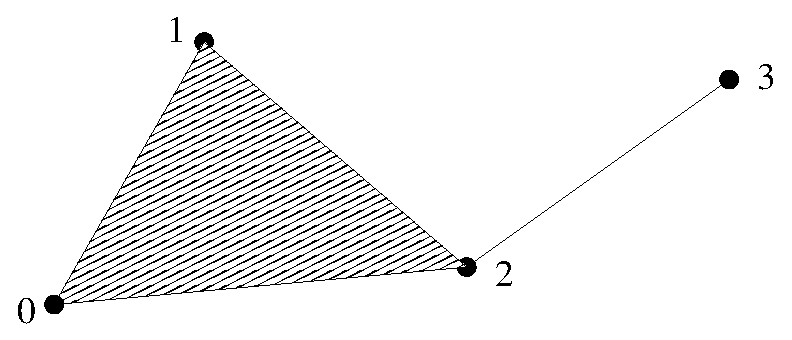
\includegraphics[scale = 0.7]{simp-gps/simp-set.eps}
%% \input{simp-set.pstex_t}
\end{center}
\begin{eqnarray*}
   V(K) &=& \{0,1,2,3\}, \\
      S &=& \{~ \{0,1,2\},~ \{2,3\},~ \{0,1\},~ \{1,2\},~ \{0,2\},~ 
             \{0\},~ \{1\},~ \{2\},~ \{3\}~ \} \\
\text{\emph{order}} &=& 2 < 1 < 3 < 0 \quad\text{\emph{(say)}},\\
(S_K)_0 &=& \{ [2],~ [1],~ [3],~ [0] \}, \\
(S_K)_1 &=& \{ [2,2]=s_0[2],~ [1,1]=s_0[1],~ [3,3]=s_0[3],~ [0,0]=s_0[0],~ 
                       [2,1],~ [2,3],~ [2,0],~ [1,0] \}, \\
(S_K)_2 &=& \{ [2,2,2]=s_0^2[2],~ [1,1,1]=s_0^2[1],~ [3,3,3]=s_0^2[3],~ 
               [0,0,0]=s_0^2[0],~ [2,2,1]=s_0[2,1],~ \\
        & &  \qquad  [2,2,3]=s_0[2,3],~ [2,2,0]=s_0[2,0],~ [2,1,1]=s_1[2,1],~ 
               [2,3,3]=s_1[2,3],~ \\ 
        & &  \qquad  [2,0,0]=s_1[2,0],~ [1,1,0]=s_0[1,0],~ [1,0,0]=s_1[1,0],~ 
               [2,1,0] \}. 
\end{eqnarray*}
\end{example}

\noindent
The face and degeneracy maps satisfy the following identities.
~{\bf [need to check these!]}  \\
The second column gives the common image of $[a_0,\ldots,a_n]$.
\begin{equation} \label{eq:face-degen} 
\begin{tabular}{ll}
$d_{j-1} \circ d_i ~=~ d_i \circ d_j\quad (0 \leqslant i < j \leqslant n)$ 
  & $\quad[a_0,\ldots,\hat{a_i},\ldots,\hat{a_j},\ldots,a_n]$, \\
$d_{j+1} \circ s_i ~=~ s_i \circ d_j\quad (0 \leqslant i < j \leqslant n)$ 
  & $\quad[a_0,\ldots,a_i,a_i,\ldots,\hat{a_j},\ldots,a_n]$, \\
$d_{i+1} \circ s_i ~=~ d_i \circ s_i ~=~ \id
\quad (0 \leqslant i \leqslant n)$ 
  & $\quad[a_0,\ldots,a_n]$, \\
$d_i \circ s_j ~=~ s_{j-1} \circ \quad (0 \leqslant i < j \leqslant n)$ 
  & $\quad[a_0,\ldots,\hat{a_i},\ldots,a_j,a_j,\ldots,a_n]$, \\
$s_{j+1} \circ s_i ~=~ s_i \circ s_j\quad (0 \leqslant i < j \leqslant n)$ 
  & $\quad[a_0,\ldots,a_i,a_i,\ldots,a_j,a_j,\ldots,a_n]$, \\
$s_{i+1} \circ s_i ~=~ s_i^2 \qquad\qquad (0 \leqslant i \leqslant n)$ 
  & $\quad[a_0,\ldots,a_i,a_i,a_i,\ldots,a_n]$. \\
\end{tabular}
\end{equation}

\bigskip\noindent
%%%%%%%%%%%%%%%%%%%%%%%%%%%%%%%%%%%%%%%%%%
{\bf The standard $n$-simplex, $\Delta^n$} 

\medskip\noindent
(See Ehlers \cite{ehlers} for some of this material.)

Let $B_{n+1} = \{\bsye_0,\ldots,\bsye_n\}$ be the standard basis for 
$\bbR^{n+1}$, and let $\Delta^n$ be the convex hull of the points $B_{n+1}$, 
a subset of the hyperplane $x_0 + x_1 + \cdots + x_n = 1$. 
The picture below shows $\Delta^2 \subseteq \bbR^3$.
\begin{center}
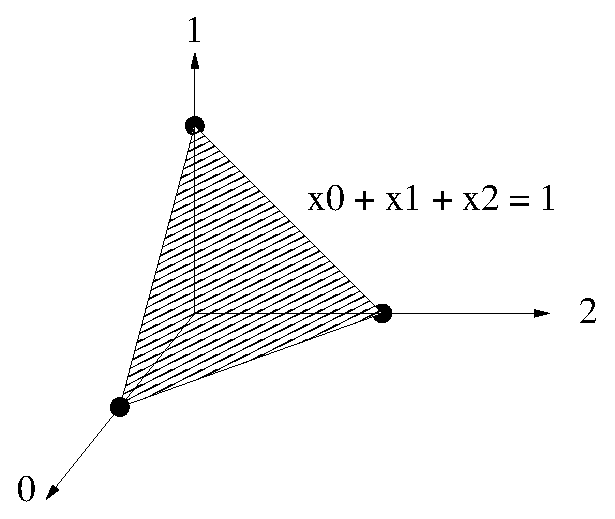
\includegraphics[scale = 0.7]{simp-gps/n-simplex.eps}
%% \input{n-simplex.pstex_t} 
\end{center}
Any $\bsyx \in \Delta^n$ may be expressed as 
$$
\bsyx ~=~ \sum_{i=0}^n\; x_i\,\bsye_i, \qquad 
\sum_{i=0}^n\;x_i ~=~ 0, \qquad x_i \geqslant 0.
$$
We then define the \emph{linear} maps 
$$
\delta_k ~:~ \Delta^{n-1} \to \Delta^n, \qquad 
(x_0,\ldots,x_{n-1}) \mapsto (x_0,\ldots,x_k,0,x_{k+1},\ldots,x_{n-1}), 
%% \bsye_i \mapsto \left\{ 
%% \begin{array}{ll} \bsye_i & (i < k), \\
%%                   \bsye_{i+1} & (i \geqslant k), 
%% \end{array} \right.
\qquad 0 \leqslant k \leqslant n. 
$$
Similarly, we define 
$$
\sigma_k ~:~ \Delta^n \to \Delta^{n-1}, \qquad 
(x_0,\ldots,x_n) \mapsto (x_0,\ldots,x_{k-1},x_k+x_{k+1},x_{k+2},\ldots,x_n), 
\qquad 0 \leqslant k \leqslant n-1. 
$$ 
The picture for $\Delta^2$ is 
\begin{center}
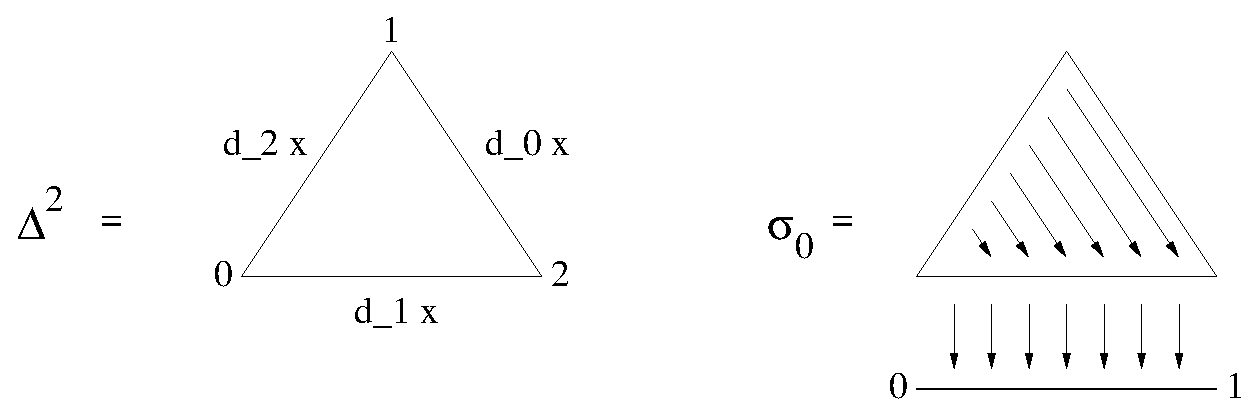
\includegraphics[scale = 0.7]{simp-gps/n-sigma.eps}
%% \input{n-sigma.pstex_t} 
\end{center}


\newpage\noindent
%%%%%%%%%%%%%%%%%%%%%%%%%%%%%%%%%%%%%%%%%%%%%%%%%%%%%
{\bf The Singular Complex $\Sing(X)$ of a space $X$.}

\medskip
For $X$ a space we defing the \emph{singular complex} of $X$ to be 
the set of maps 
$$
\Sing(X) ~=~ \Top(\Delta^n,X). 
$$

The diagram below shows such a map $\tau$ to a space $X$ with two holes.
\begin{center}
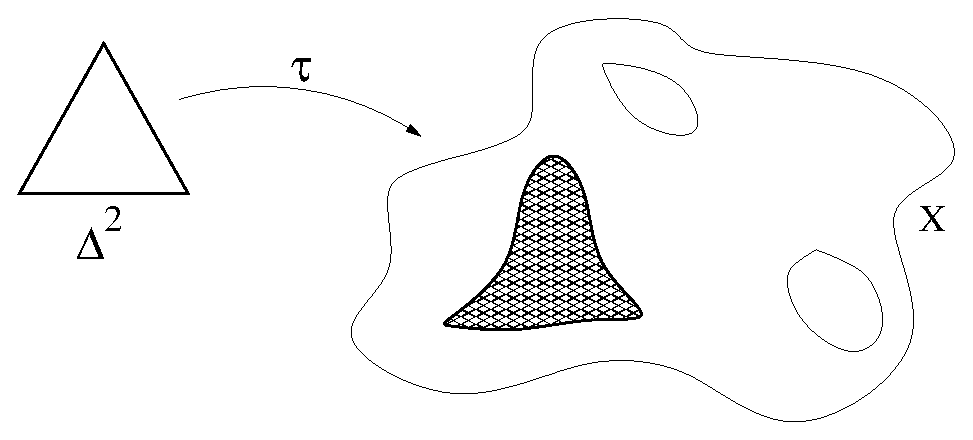
\includegraphics[scale = 0.7]{simp-gps/delta2X.eps}
%% \input{delta2X.pstex_t} 
\end{center}


\bigskip\noindent
{\bf The Nerve of a Category} 

\medskip/noindent
Let $\bbC$ be a small category. 
The \emph{nerve} of $\bbC$ is defined to be the simplicial set $\Ner\,\bbC$ 
where 
\begin{itemize}
\item~~
$(\Ner\,\bbC)_0 = \Ob(\bbC)$, 
\item~~
$(\Ner\,\bbC)_1 = \Arr(\bbC)$, 
\item~~
for $x \in (\Ner\,\bbC)_1$, $d_0 x = tx$ and $d_1x = hx$, 
\item~~
for $u \in (\Ner\,\bbC)_0$, $s_0u = 1_u$, 
\item~~
$(\Ner\,\bbC)_n = \{ \text{composable words}~ (x_1,\ldots,x_n) ~|~  
                    x_i \in \Arr(\bbC) \}$, 
\item~~
$d_0(x_1,x_2,\ldots,x_n) ~=~ (x_2,\ldots,x_n)$, 
\item~~
$d_i(x_1,\ldots,x_n) ~=~ (x_1,\ldots,x_ix_{i+1},\ldots,x_n), \quad (0<i<n)$, 
\item~~
$d_n(x_1\ldots,x_{n-1},x_n) ~=~ (x_1,\ldots,x_{n-1})$, 
\item~~
$s_0(x_1,\ldots,x_n) ~=~ (1_{tx_0},x_1,\ldots,x_n)$, 
\item~~
$s_i(x_1,\ldots,x_n) ~=~ (x_1,\ldots,x_i,1_{hx_i},x_{i+1},\ldots,x_n), 
\quad (0<i<n)$, 
\item~~
$s_n(x_1,\ldots,x_n) ~=~ (x_1,\ldots,x_n,1_{hx_n})$. 
\end{itemize}

This may be described more compactly by saying that 
$(\Ner\,\bbC)_n = \Cat([n],\bbC)$. 
This construction extends to a functor from $\Cat$ to $\SimpSet$ 
in the obvious way. 

 




%% crossed n-cubes of groups 
\newpage %% xncube.tex, version 03/05/17


%%%%%%%%%%%%%%%%%%%%%%%%%%%%%%%%%%%%%%%%%%%%%%%%%%%%%%%%%
\section{Crossed $n$-cubes of groups and cat$^n$-groups}

\noindent
Here we include the basic ideas about crossed $n$-cubes (of groups)
taken from Chapter 1 of Ellis' thesis \cite{ellis-thesis},
Ellis-Steiner \cite{ell:st}, and Brown-Loday \cite{brow:lod}, 
and the associated cat$^n$-groups.


%%%%%%%%%%%%%%%%%%%%%%%%%%%%%%%%%%%%%%%%
\subsection{Crossed $n$-cubes of groups}  \index{crossed $n$-cube}

Let $[n] = \{1,2,...,n\}$, and let $A,B,C,\ldots$ be subsets of $[n]$.

\bigskip
A crossed $n$-cube consists of the following.
\begin{enumerate}[(i)]
\item
Groups  $R_A$  for each subset  $A$  of  $[n]$,
where we write $R$ for $R_{\emptyset}$.

\item
Group homomorphisms
$$
\partial_{A,i} : R_A \to R_{A \setminus \{i\}}  \quad\mbox{for all} \quad 
A \subseteq [n],~ i \in A, 
$$
such that  
$\partial_{A \setminus \{j\},i} \circ \partial_{A,j} 
~=~ \partial_{A \setminus \{i\},j} \circ \partial_{A,i} 
~\mbox{for}~ i \neq j \in A$.

\noindent
Since the $\partial_{A,i}$ commute, composite homomorphisms
$\partial_{A,B} : R_A \to R_{A \setminus B}$ are well defined and 
$\partial_{A,B} = \partial_{A,(B \setminus C)} \circ \partial_{A,C}$. 

\item
For all $B \subseteq A$ an action of $R_{A \setminus B}$ on $R_A$
making $\calR_{A,A \setminus B} = (\partial_B : R_A \to R_{A \setminus B})$
a crossed module.

For each $j \in [n]$ the maps 
$$
(1,\partial_{A \ setminus \{i\}},j) : \calR_{A,A \setminus \{i\}} \to 
\calR_{A,A \setminus \{i,j\}}
\quad\mbox{and}\quad
(\partial_{A,j},1) : \calR_{A,A \setminus \{i,j\}} \to 
\calR_{A \setminus \{j\},A \setminus \{i,j\}}
$$
are crossed module homomorphisms.

It follows that all the actions act via $R$~:
$$
a^b ~=~ a^{\partial_{B,B} b} \quad\mbox{for}\quad
a \in R_A,~ b \in R_B, ~~\mbox{and}~~ B \subseteq A.
$$

\item
For all  $A,B \subseteq [n]$  a crossed pairing  ~
$\bt_{A,B} : R_A \times R_B \to R_{A \cup B}$~,
such that
$(b\,\bt_{B,A}\,a) = (a\,\bt_{A,B}\,b)^{-1}$  and, when $B \subseteq A$,
$\bt_{A,B}$  is the principal crossed pairing for $\calR_{A,B}$ 
given by ~$a \bt b = a^{-1}a^b$ and $b \bt a = (a^{-1})^ba$.

\item
Various axioms relating the homomorphisms, actions, and crossed pairings, 
for example
\begin{itemize}
\item~ $\partial_{A \cup B,i}(a \bt_{A,B} b) = 
    (\partial_{A,i} a) \bt_{A\setminus\{i\},B\setminus\{i\}} (\partial_{B,i} b)$.
\item~ when $i \in A \cap B$, so that
$A \cup B = (A \setminus \{i\}) \cup B = A \cup (B \setminus \{i\})$,
$$
a \bt_{A,B} b
~=~ \partial_{A,i} a \bt_{A,B\setminus\{i\}} b
~=~ a \bt_{A\setminus\{i\},B} \partial_{B,i} b.
$$
(This means that we need only define $\bt_{A,B}$ when $A \cup B = \emptyset$.)
\item~ $(a \bt b)^c ~=~ a^c \bt b^c$ when $C \subseteq A$ and $C \subseteq B$.
\qquad
\mbox{{\bf [Is this correct?]}}
\end{itemize}
\end{enumerate}

\bigskip
We might now wish to define an \emph{$n$-derivation}, 
which would seem to be a set of maps
$$
\chi_{B,A} : R_B \to R_A  \quad\mbox{for all}\quad  B \subseteq A
$$
satifying suitable axioms:
\begin{enumerate}[(i)]
\item
perhaps  \qquad 
$\chi_{B,A}(bb') = (\chi_{B,A} b)^{b'} (\chi_{B,A} b')$ ~?
\item
closure: \qquad
$\chi_{B,A} \circ \chi_{C,B} = \chi_{C,A}$ ~?
\item ???
\end{enumerate}

\begin{exercise}
\emph{Derive the crossed square axioms 
from those of a crossed $2$-cube.}
\end{exercise}


\bigskip\noindent
{\bf [These are just some thoughts to be worked on!]}



%%%%%%%%%%%%%%%%%%%%%%%%%%%
\subsection{Cat$^n$-groups}  \index{cat$^n$-group} 

As with cat$^2$-groups (see \ref{subs:cattwo}), 
we will give three definitions. 

\begin{defn} \label{def:catna}
\emph{A cat$^n$-group consists of the following.} 
\begin{enumerate}[(i)]
\item
\emph{$2^n$ groups  $G_A$, one for each subset  $A$  of  $[n]$, 
the \emph{vertices} of a cube.} 
\item
\emph{Group homomorphisms forming $n2^{n-1}$ commuting cat$^1$-groups,} 
$$
\calC_{A,i} = (e_{A,i};\ t_{A,i},\ h_{A,i} : G_A \to G_{A \setminus \{i\}}), 
\quad\mbox{\emph{for all}} \quad A \subseteq [n],~ i \in A,  
$$
\emph{the \emph{edges} of the cube.} 
\item 
\emph{These cat$^1$-groups combine (in sets of $4$) 
to form $n(n-1)2^{n-3}$ cat$^2$-groups $\calC_{A,\{i,j\}}$ 
for all $\{i,j\} \subseteq A \subseteq [n],~ i \neq j$, 
the \emph{faces} of the cube.} 
\end{enumerate}
\end{defn}
Note that, since the $t_{A,i}, h_{A,i}$ and $e_{A,i}$ commute, 
composite homomorphisms
$t_{A,B}, h_{A,B} : G_A \to G_{A \setminus B}$ and 
$e_{A,B} : G_{A \setminus B} \to G_A$ 
are well defined for all $B \subseteq A \subseteq [n]$.  

\medskip 
Secondly, we give the simplest of the three definitions, 
again adapted from Ellis-Steiner \cite{ell:st}. 
\begin{defn} \label{defn:catnb} 
\emph{A cat$^n$-group  $\calC$ consists of $2^n$ groups 
$G_A$, one for each subset  $A$  of  $[n]$, 
and $3n$ homomorphisms 
$t_{[n],i}, h_{[n],i} : G_{[n]} \to G_{n \setminus \{i\}},~ 
 e_{[n],i} : G_{[n] \setminus \{i\}} \to G_{[n]}$,  
satisfying the following axioms for all $1 \leqslant i \leqslant n$,}  
\begin{enumerate}[(a)]
\item~ \emph{the 
$
\calC_{[n],i} = (e_{[n],i};t_{[n],i},h_{[n],i}:G_{[n]} \to G_{[n] \setminus \{i\}}) 
$
are \emph{commuting} cat$^1$-groups, so that:} 
\item~ 
$
(e_1 \circ t_1) \circ (e_2 \circ t_2) = (e_2 \circ t_2) \circ (e_1 \circ t_1), \quad
(e_1 \circ h_1) \circ (e_2 \circ h_2) = (e_2 \circ h_2) \circ (e_1 \circ h_1), 
$
\item~ 
$
(e_1 \circ t_1) \circ (e_2 \circ h_2) = (e_2 \circ h_2) \circ (e_1 \circ t_1), \quad 
(e_2 \circ t_2) \circ (e_1 \circ h_1) = (e_1 \circ h_1) \circ (e_2 \circ t_2). 
$
\end{enumerate}
\end{defn} 

\medskip 
Our third definition defines a cat$^n$-group as a 
"cat$^1$-group of cat$^{(n-1)}$-groups". 
\begin{defn} \label{defn:catnc} 
\emph{A cat$^n$-group $\calC$ consists of two cat$^{(n-1)}$-groups:} 
\begin {itemize} 
\item
\emph{$\calA$ with groups $G_A, A \subseteq [n-1]$, 
and homomorphisms $\ddtt_{A,i}, \ddhh_{A,i}, \ddee_{A,i}$,} 
\item 
\emph{$\calB$ with groups $H_B, B \subseteq [n-1]$,
and homomorphisms $\dtt_{B,i}, \dhh_{B,i}, \dee_{B,i}$,} 
\item 
\emph{and cat$^{(n-1)}$-morphisms $t,h : \calA \to \calB$ 
and $e : \calB \to \calA$
subject to the following conditions:} 
\begin{center}
\begin{tabular}{r l}
\textbf{C1:}  &  \emph{$(t \circ e)$ and $(h \circ e)$~ 
                 are the identity mapping on~ $\calB$,} \\
\textbf{C2:}  &  $[\ker t, \ker h] = \{ 1_{\calA} \}$.
\end{tabular}
\end{center}
\end{itemize}
\end{defn}




%% other types of crossed module 
\newpage %% acc-lie-alg.tex,  version 22/05/21

%%%%%%%%%%%%%%%%%%%%%%%%%%%%%%%%%%%%%%%%%%%%%%%%%%%%%%%%%%%%%%%%%%%%%%%%%%%%
\section{Other types of Crossed Module}

This chapter needs a lot of work. 

\bigskip

Ellis, in \cite{ellis-thesis}, defined crossed modules, cat$^1$-groups, 
and associated structures in \emph{categories of $\Omega$-groups} which, 
as well as including ordinary groups, includes associative algebra 
and Lie algebras. 
In this section we describe the constructions in these two particular cases. 


%%%%%%%%%%%%%%%%%%%%%%%%%%%%%%%%%%%%%%%%%%%%%%%%%%%
\subsection{Crossed modules of associative algebras and cat$^1$-algebras}

This material is adapted from Arvasi and Odabas \cite{arv:oda}.









%%%%%%%%%%%%%%%%%%%%%%%%%%%%%%%%%%%%%%%%%%%%%%%%%%%
\subsection{Crossed modules of Lie algebras}

This material is adapted from Casas and Ladra \cite{casas:ladra}.




%%%%%%%%%%%%%%%%%%%%%%%%%%%%%%%%%%%%%%%%%%%%%%%%%%%
\subsection{Representations of crossed modules}

This material is adapted from Forrester-Barker \cite{f-b-thesis}.






%% 2-groupoid enrichments 
\newpage %% 2gpd.tex,  version 01/05/17


%%%%%%%%%%%%%%%%%%%%%%%%%%%%%%%%%%%%%
\section{2-groupoid enrichments}

\noindent
{\bf How does a group act on a set?}

Let $G$ be a group (thought of as a $1$-object groupoid) 
and $X$ a set (with $0$ groupoid structures). 
Construct the ($1$-)groupoid $\Symm(X)$, 
whose arrows form the group of permutations of $X$.
An action of $G$ on $X$ is then determined by a groupoid homomorphism 
$\theta : G \to \Symm(X)$.

We now form a cat$^0$-group $X_G$ (which is just a group) from $G$, 
by throwing away the single object, 
leaving a set with extra structure (the group multiplication). 
We then require the subgroupoid of $\Symm(X_G)$ whose arrows 
are the permutations which preserve the multiplication. 
This subgroupoid is of course $\Aut(G)$. 
The inner morphism $\iota$, mapping $g \in G$ to conjugation by $g$, 
gives an action of $G$ on itself. 
The actor crossed module of $G$ is then $(\iota : G \to \Aut(G))$, 
which can be thought of as a cat$^1$-group, 
or group-groupoid, or $2$-groupoid.

\bigskip\noindent
{\bf How does a crossed module act on a groupoid?} 

Let $\calX$ be a crossed module, 
thought of as a $2$-groupoid $\calG$ with one object, 
and let $\Gamma$ be a groupoid. 
Construct the $2$-groupoid $\Symm(\Gamma)$, with one object $\bullet$, 
the automorphisms of $\Gamma$ as arrows, 
thought of as functors $\Gamma \to \Gamma$, 
and natural transformations between these functors as $2$-cells. 
An action of $\calX$ on $\Gamma$ is then determined by a 
$2$-groupoid homomorphism $\theta : \calG \to \Symm(\Gamma)$.

We now form a cat$^1$-group (group-groupoid) $\Gamma_{\calX}$ from $\calX$ 
by throwing away the single object, 
leaving a groupoid with extra structure (again group multiplication).
We then require the sub-$2$-groupoid $\Act(\calX)$ 
of $\Symm(\Gamma_{\calX})$ whoses arrows 
are the automorphims which preserve the cat$^1$-structure 
(and whose $2$-cells preserve ???). 
The inner morphism $\iota : \calX \to \Act(\calX)$ then has to be determined.  
The actor crossd square of $\calX$ is then 
$(\iota : \calX \to \Act(\calX))$, 
which can be thought of as a cat$^2$-group, 
or $3$-groupoid, or group-double groupoid (is this correct?), or whatever.

\bigskip\noindent 
{\bf How does a crossed square act on a double groupoid?} 

Let $\calS$ be a crossed square, thought of as a $3$-groupoid, 
and let $\calD$ be a double groupoid. 
Construct the $3$-groupoid $\Symm(\calD)$ 
(or should this be a $2$-double groupoid?)
with one object, whose arrows are automorphisms of $\calD$ (double functors), 
$2$-cells are homotopies, or double natural transformations (?), 
and $3$-cells are $2$-homotopies of some sort? 
An action of $\calS$ on $\calD$ is then determined by a 
$3$-groupoid homomorphism $\theta : \calS \to \Symm(\calD)$.

We now form a cat$^2$-group (group-double groupoid) 
$\calD_{\calS}$ from $\calS$ by throwing away the single object, 
leaving a double groupoid with extra structure (again group multiplication).
We then require the sub-$3$-groupoid $\Act(\calS)$ 
of $\Symm(\calD_{\calS})$ whoses arrows 
are the automorphims which preserve the cat$^2$-structure 
(and whose $2$-cells and $3$-cells preserve ???). 
The inner morphism $\iota : \calS \to \Act(\calS)$ then has to be determined.  
The actor crossd cube of $\calS$ is then 
$(\iota : \calS \to \Act(\calS))$, 
which can be thought of as a cat$^3$-group, 
or $4$-groupoid, or group-triple groupoid (is this also correct?) 
and, no doubt, lots of other gadgets in the crossed menagerie!


\newpage
%%%%%%%%%%%%%%%%%%%%%%%%%%%%%%%%%%%%%%%%%%%%%%%%%%%%%
\subsection{The automorphism 2-category of a 2-group}

This material is adapted from \cite{kamps:port}.

Let $\calG$ be the ``$2$-group associated to the crossed module 
$\calX = (\partial : S \to R)$'', 
as described in Subsection \ref{subs:twogps}, 
with $2$-cells

$$
\xy
\xymatrix{
  && && \\
  \bullet  \ar@/^5ex/[rrrr]^{r} 
           \ar@/_5ex/[rrrr]_{r(\partial s)} 
  && \Downarrow (r,s)
     && \bullet \\
  && && \\
}
\endxy
$$

\medskip\noindent
We now seek to describe $\calF = \calF(\calG,\calG)$, 
the automorphism $2$-category of $\calG$.

\medskip\noindent
{\large{\bf objects of $\calF$}}\\ 
These are strict $2$-functors $\beta,\gamma,\ldots : \calG \to \calG$, 
where we write $\beta = (\id_{\bullet},\db, \barb=(\db,\ddb))$, 
mapping $\bullet$ to itself, $r$ to $\db r$, 
and $(r,s)$ to $(\db r, \ddb s)$. 
Of course $\db,\ddb$ are automorphisms of $R,S$ respectively. 
(Perhaps generalise to endomorphisms.)
Since $\beta$ is a $2$-functor, tail and head maps are preserved, 
so $\partial\ddb = \db\partial$.

\medskip\noindent
{\large{\bf $1$-arrows of $\calF$}}\\
These have the form $\barch : \beta \to \gamma$, 
and are $2$-natural transformations which make the following assignments. 
To the object $\bullet$ we assign an element 
$q = q_{\beta}^{\gamma} = \barch(\bullet) \in R$.

\noindent
To $r \in R$ we assign a square $2$-cell
$$
%\vcenter{
{\xy
\xymatrix{
  \bullet \ar[rr]^{\db r} 
    & \ar @{=>} [dr]_{\barch r}
      & \bullet 
        & & \\
    & & & \equiv
          & \\
  \bullet \ar[uu]^q \ar[rr]_{\dg r} 
    & & \bullet \ar[uu]_q
        & & \\
}
\endxy}
{\xy
\xymatrix{
  && && \\
  \bullet  \ar@/^5ex/[rrrr]^{q(\db r)} 
           \ar@/_5ex/[rrrr]_{(\dg r)q} 
  && \Downarrow\, \barch r
     && \bullet \\
  && && \\
}
\endxy}
%}
$$
where 
$\barch r = \barch_{\beta}^{\gamma} r = (q(\db r),\ddch r) \in R \ltimes S$, 
say.
Since $\barch r$ has head $(\dg r)q$, we have
\begin{equation} \label{eq:partial-ddch-r} 
(\db r)(\partial \ddch r) ~=~ (\dg r)^q \quad\mbox{in}~R,
\end{equation}
so that $\partial \ddch r$ measures the amount by which the square 
does not commute.

\medskip\noindent
The squares $\barch r$, for $r \in R$, are required to satisfy three axioms.
\begin{enumerate}[(i)]
\item
For the identity in $R$ we have $\barch 1_R = \Downarrow(1,q)$, 
the vertical identity $2$-cell at $q$.
\item
Product in $R$ is preserved: $\barch(r_1 \sharpz r_2)$ corresponds to 
the vertical composite $\barch r_1 \star_0 \barch r_2$ 
shown in the following diagram.
$$
{\vcenter 
{\xy
\xymatrix{
  \bullet \ar[rr]^{\db r_1} 
    & \ar @{=>} [dr]_{\barch r_1} 
      & \bullet \ar[rr]^{\db r_2} 
        & \ar @{=>} [dr]_{\barch r_2}  
          & \bullet \\
    & & & & \\
  \bullet \ar[uu]^q \ar[rr]_{\dg r_1}  
    & & \bullet \ar[uu]_q \ar[rr]_{\dg r_2}  
        & & \bullet \ar[uu]_q \\
}
\endxy}
\quad=\quad
{\xy
\xymatrix @C=1.5pc{
    & & & & & \\
  \bullet  \ar@/^5ex/[rr]^{q(\db r_1)} 
           \ar@/_5ex/[rr]_{(\dg r_1)q} 
    & \Downarrow\, (q(\db r_1), \ddch r_1)
       & \bullet \ar[r]^{q^{-1}} 
          & \bullet \ar@/^5ex/[rr]^{q(\db r_2)} 
                    \ar@/_5ex/[rr]_{(\dg r_2)q} 
              & \Downarrow\, (q(\db r_2), \ddch r_2) 
                   & \bullet \\
    & & & & & \\
}
\endxy}
}$$
The composite of these is
$$
\xy
\xymatrix @C=1.8pc{
  && && \\
  \bullet  \ar@/^5ex/[rrrr]^{q(\db r_1)(\db r_2)} 
           \ar@/_5ex/[rrrr]_{(\dg r_1)(\dg r_2)q} 
  && \Downarrow\, (q(\db r_1)(\db r_2), (\ddch r_1)^{\db r_2}(\ddch r_2))
      && \bullet \\
  && && \\
}
\endxy
$$
This composite $2$-cell is required to be be equal to
$$
{\vcenter 
{\xy
\xymatrix{
  \bullet \ar[rr]^{\db(r_1r_2)} 
    &  \ar @{=>} [dr]_{\barch(r_1r_2)} 
      & \bullet \\
    & & \\
  \bullet \ar[uu]^q \ar[rr]_{\dg(r_1r_2)} 
    & & \bullet \ar[uu]_q \\
}
\endxy} 
\quad\equiv\quad 
{\xy
\xymatrix{
    && && \\
    \bullet \ar@/^5ex/[rrrr]^{q\db(r_1r_2)} 
            \ar@/_5ex/[rrrr]_{\dg(r_1r_2)q} 
    && \Downarrow\, (q\db(r_1r_2),\ddch(r_1r_2))
       && \bullet \\
    && && \\
}
\endxy}
}$$
We deduce that $\ddch$ is a $\beta$-derivation:
$$
\ddch(r_1r_2) ~=~ (\ddch r_1)^{\db r_2}\;(\ddch r_2).
$$

\item
If $(r,s) : r \to r(\partial s)$ then $(\barb(r,s),\barg(r,s))$ forms a 
vertical homotopy from $\barch r$ to $\barch(r(\partial s))$. 
This means that the following composite $2$-cells are equal. 
$$
{\vcenter 
{\xy
\xymatrix @C=1.6pc{ 
    & & & & \\
  \bullet \ar@/^5ex/[rrrr]^{\db r}
    & & & \ar@{=>} [dr]_{\barch r}
          & \bullet \\
    & & & & \\
  \bullet \ar[uu]^q \ar@/^5ex/[rrrr]^{\dg r}
          \ar@/_5ex/[rrrr]_{\dg(r(\partial s))}
    & & \Downarrow(\dg r,\ddg r)
        & & \bullet \ar[uu]_q \\
    & & & & \\
}
\endxy}
\qquad=\qquad
{\xy 
\xymatrix @C=1.6pc@R=0.9pc{ 
    & & & & \\ 
  \bullet \ar@/^5ex/[rrrr]^{\db r} \ar@/_5ex/[rrrr]_{\db(r(\partial s))}
    & & \Downarrow(\db r,\ddb r)
        & & \bullet \\
    & & & \ar@{=>} [ddr]_{\barch(r(\partial s))}
          & \\ 
    & & & & \\
    & & & & \\ 
  \bullet \ar[uuuu]^q \ar@/_5ex/[rrrr]_{\dg(r(\partial s))}
    & & & & \bullet \ar[uuuu]_q \\ 
    & & & & \\ 
}
\endxy}
}$$
It follows that
\begin{eqnarray*}
       (\barch r) \sharpo ((\dg r,\ddg s) \sharpz q)
 & = & (q \sharpz (\db r,\ddb s)) \sharpo \barch(r(\partial s)), \\
       (q(\db r),\ddch r) \sharpo ((\dg r)q,(\ddg s)^q)
 & = & (q(\db r),\ddb s) \sharpo (q\db(r(\partial s)),\ddch(r(\partial s))), \\
       (q(\db r), (\ddch r)(\ddg s)^q) 
 & = & (q(\db r),(\ddb s)(\ddch r)^{\db\partial s}(\ddch\partial s)), \\ 
       (\ddch r)(\ddg s)^q 
 & = & (\ddb s)(\ddch r)^{\partial\ddb s}(\ddch\partial s), \\
       (\ddch r)(\ddg s)^q 
 & = & (\ddch r)(\ddb s)(\ddch\partial s), 
\end{eqnarray*}
which gives the identity (compare with equation (\ref{eq:partial-ddch-r}))
\begin{equation} \label{eq:ddch-partial-r} 
(\ddg s)^q  ~=~  (\ddb s)(\ddch\partial s),~~ 
\end{equation}
which shows that $\ddch \partial s$ measures the amount by which 
$(\ddg s)^q$ differs from $\ddb s$.
\end{enumerate}

\medskip
The composite $\barch_{\beta}^{\delta}$ 
of $\barch_{\beta}^{\gamma} : \beta \to \gamma$ 
with $\barch_{\gamma}^{\delta} : \gamma  \to \delta$, 
is shown in the following diagram.
$$
{(\barch_{\beta}^{\gamma} r) \star_1 (\barch_{\gamma}^{\delta} r)}
{\quad=\quad}
{\xy
\xymatrix{
  \bullet \ar[rr]^{\db r} 
    & \ar @{=>} [dr]_{\barch_{\beta}^{\gamma} r}
      & \bullet \\
    & & \\
  \bullet \ar[uu]^{q_{\beta}^{\gamma}} 
          \ar[rr]^(0.3){\dg r} 
    & \ar @{=>} [dr]_{\barch_{\gamma}^{\delta} r} 
      & \bullet \ar[uu]_{q_{\beta}^{\gamma}} \\
    & & \\
  \bullet \ar[uu]^{q_{\gamma}^{\delta}} \ar[rr]_{\dd r} 
    & & \ar[uu]_{q_{\gamma}^{\delta}} \\
}
\endxy}
{\quad=\quad} 
{(q_{\gamma}^{\delta} \sharpz (\barch_{\beta}^{\gamma} r)) 
\sharpo
((\barch_{\gamma}^{\delta} r) \sharpz (q_{\beta}^{\gamma})),} 
$$
so that
$$
\barch_{\beta}^{\delta}(\bullet) \;=\; q_{\gamma}^{\delta}q_{\beta}^{\gamma}
\qquad\mbox{and}\qquad
\barch_{\beta}^{\delta}(r) \;=\; \Downarrow 
(q_{\gamma}^{\delta}q_{\beta}^{\gamma}(\db r), 
 (\chi_{\beta}^{\gamma}r)(\chi_{\gamma}^{\delta}r)^{q_{\beta}^{\gamma}}).
$$


\medskip
Suppose there exists $s \in S$ such that $\partial s = q$. 
Then, using the principal $\gamma$-derivation $\eta_s$, 
we may define the \emph{principal $2$-cell} 
$\bare_{\gamma}^{\gamma} r = (q(\dg r),\eta_s r)$ 
with tail $q(\dg r)$ and head 
$$
q(\dg r) \partial((s^{-1})^{\dg r}s)
 \;=\; q(\dg r)(q^{-1})^{\dg r}q 
 \;=\; (\dg r)q~.
$$


\bigskip\noindent
{\large{\bf $2$-arrows of $\calF$}}\\
To $\barch,\barch' \in \calF$



%% oddments
\newpage %% oddments.tex,  version 21/05/21

%%%%%%%%%%%%%%%%%%
\section{Oddments}

This chapter is a place to include experimental material.

\bigskip

%%%%%%%%%%%%%%%%%%%%%%%%%%%%%%%%%%%%%%%%%%%%%%%%%%%%%%%%%%%%%%%%%%%%%%%%
\subsection{Actor of a 2-fold crossed module} \label{subs:actor-xxmod}

\begin{defn} \index{Whitehead group} \index{regular derivation} 
The Whitehead group $W_1(\calR)$ is defined to be the group of the monoid 
$\Der_1(\calR)$. 
Elements of $W_1(\calR)$ are called regular derivations.
\end{defn}

\noindent
The following result is a higher-dimensional version of
Lemma \ref{lem:chi-sigma-rho}.

\begin{lem} \label{lem:equiv-w1s}
The following statements are equivalent 
\begin{enumerate}[\rm (a)]
\item $\chi = (\ddch, \dch) \in W_1(\calR) $
\item $\sigma_{\chi} = (\dds_{\chi}, \ds_{\chi})  \in \Aut(\ddcalRt)$
\item $ \rho_{\chi} = (\ddr_{\chi}, \dr_{\chi})  \in \Aut(\dcalRt)$
\end{enumerate}
\end{lem}
\begin{pf}
Here is an incomplete argument.
Assume that $\sigma_{\chi}, \rho_{\chi}$ are invertible.
Then, by Lemma \ref{lem:chi-sigma-rho}, 
$$
\ddch^{-1}n ~=~ (\dds_{\chi}^{-1}\ddch n)^{-1} 
            ~=~ (\ddch\ddr_{\chi}^{-1} n)^{-1}
\qquad\mbox{and}\qquad
\dch^{-1}p ~=~ (\ds_{\chi}^{-1}\dch p)^{-1} 
           ~=~ (\dch\dr_{\chi}^{-1} p)^{-1},
$$
and hence
$$
\ddbdy_2 \circ \ddch^{-1} (n)
~=~ (\ddbdy_2 \dds_{\chi}^{-1} \ddch n)^{-1}
~=~ (\ds_{\chi}^{-1} \ddbdy_2 \ddch n)^{-1}
~=~ (\ds_{\chi}^{-1} \dch \dbdy_2 n)^{-1}
~=~ \dch^{-1} \circ \dbdy_2 (n).
$$
So $\chi^{-1} = (\ddch^{-1},\dch^{-1}) \in W_1(\calR)$.
\end{pf}

\begin{defn}
The group $\Aut(\calR)$ of automorphisms of the crossed square $\calR$ is 
$$
\Aut(\calR) ~=~ \{ \alpha = 
(\alpha_{[2]}, \alpha_{\{1\}}, \alpha_{\{2\}}, \alpha_{\emptyset}) \}
$$ 
such that 
$(\alpha_{[2]}, \alpha_{\{1\}}) $  is an automorphism of  $\ddcalRt$,
$(\alpha_{[2]}, \alpha_{\{2\}}) $  is an automorphism of  $\ddcalRo$,
$(\alpha_{\{2\}}, \alpha_{\emptyset}) $  is an automorphism of  $\dcalRt$, and 
$(\alpha_{\{1\}}, \alpha_{\emptyset}) $  is an automorphism of  $\dcalRo$.
\end{defn}

\begin{lem} \label{lem:alpha-chi}
If $\chi \in \Der_1(\calR)$ then
$\alpha_{\chi} = (\dds,\ds,\ddr,\dr) \in \Aut(\calR)$
where
$$
\dds \ell = \ell(\ddch \ddbdyo \ell), \quad
\ds m = m(\dch \dbdyo m), \quad
\ddr n = n(\ddbdyo \ddch  n), \quad
\dr p = p(\dbdyo \dch p). 
$$
\end{lem}
\begin{pf}
This follows immediately from Lemma \ref{lem:equiv-w1s}.
\end{pf}

\begin{lem} 
There is a crossed module
$$
\calA_1{\calR} ~=~ (\dD_1 : W_1(\calR) \to \Aut(\calR), ~
\chi \mapsto \alpha_{\chi})
$$
where the action of $\Aut(\calR)$ on $W_1(\calR)$ is given by
$\chi^{\alpha} = \psi = (\ddps, \dps)$
where 
$$ 
\ddps : R_{\{2\}} \to R_{[2]}  \;=\; \alpha_{\{2\}}^{-1} * \ddch * \alpha_{[2]},
\quad \mbox{and} \quad  
\dps : R_{\emptyset} \to R_{\{1\}}  \;=\; 
\alpha_{\emptyset}^{-1} * \dch * \alpha_{\{1\}}.
$$
\end{lem}
\begin{pf}
We first show that the boundary map $\dD_1$ is a homomorphism.
The proof is the same as the proof of Lemma 3.3 in the notes.

Secondly we must show that the action is well-defined.
\begin{eqnarray*}
(\chi^{\alpha})^{\beta} 
  & = & ((\alpha_{\{2\}}^{-1} * \ddch * \alpha_{[2]})^{\psi_2}, \,  
        (\alpha_{\emptyset}^{-1} * \dch * \alpha_{\{1\}})^{\psi_2})  \\
  & = & (\beta_{\{2\}}^{-1} * (\alpha_{\{2\}}^{-1} * \ddch 
        * \alpha_{[2]}) * \beta_{[2]},\,
         \beta_{\emptyset}^{-1} * (\alpha_{\emptyset}^{-1} * \dch 
        * \alpha_{\{1\}}) * \beta_{\{1\}} )\\
  & = & ((\alpha_{\{2\}} \beta_{\{2\}})^{-1} * \ddch 
        * (\alpha_{[2]} \beta_{[2]}), \,  
         (\alpha_{\emptyset} \beta_{\emptyset})^{-1} * \dch 
        * (\alpha_{\{1\}} \beta_{\{1\}})) \\
  & = & \chi^{\alpha*\beta}
\end{eqnarray*}

Thirdly we show that $\psi = \chi^{\alpha}$ commutes with 
$\partial_1 = (\ddbdyo,\dbdyo)$, so that  $\dps \dbdyo = \ddbdyo \ddps$.
\begin{eqnarray*}
(\dps \dbdyo)(n) 
  & = & (\alpha_{\emptyset}^{-1} * \dch * \alpha_{\{1\}})(\dbdyo n) \\
  & = & (\alpha_{\{1\}} \dch \alpha_{\emptyset}^{-1})(\dbdyo n) \\
  & = & \alpha_{\{1\}} \dch \dbdyo \alpha_{\{2\}}^{-1} n \\
  & = & \alpha_{\{1\}} \ddbdyo \ddch \alpha_{\{2\}}^{-1} n \\
  & = & \ddbdyo \alpha_{[2]} \ddch \alpha_{\{2\}}^{-1} n \\
  & = & \ddbdyo(\alpha_{\{2\}}^{-1} \star \ddch \star \alpha_{[2]})(n) \\
  & = & \ddbdyo \ddps (n)~. \\
\end{eqnarray*}

Now we verify the first crossed module axiom,~
$\dD_1(\chi^{\alpha}) = \alpha^{-1} * \dD_1 \chi * \alpha$~
where
\begin{eqnarray*}
\alpha^{-1} * \dD_1\chi * \alpha 
  & = & (\alpha_{[2]}, \alpha_{\{1\}}, \alpha_{\{2\}}, 
         \alpha_{\emptyset})^{-1} * (\dds_{\chi}, 
        \ds_{\chi}, \ddr_{\chi}, \dr_{\chi}) 
        * (\alpha_{[2]}, \alpha_{\{1\}}, \alpha_{\{2\}}, \alpha_{\emptyset}) \\
  & = & (\alpha_{[2]}^{-1} * \dds_{\chi} * \alpha_{[2]}, \ 
         \alpha_{\{1\}}^{-1} * \ds_{\chi} * \alpha_{\{1\}}, \ 
         \alpha_{\{2\}}^{-1} * \ddr_{\chi} 
        * \alpha_{\{1\}}, \ \alpha_{\emptyset}^{-1} * \dr_{\chi} 
        * \alpha_{\emptyset})
\end{eqnarray*}
We verify just the first and the last coordinate, since the other two
are similar.
\begin{eqnarray*}
\dds_{\psi} \ell 
  & = & \ell(\ddps \ddbdyo \ell) \\
  & = & \ell(\alpha_{\{2\}}^{-1} * \ddch * \alpha_{[2]})(\ddbdyo \ell) \\
  & = & \ell (\alpha_{[2]}  \ddch  \alpha_{\{2\}}^{-1} \ddbdyo \ell) \\
  & = & \ell (\alpha_{[2]}  \ddch \ddbdyo  \alpha_{[2]}^{-1} \ell) \\
(\alpha_{[2]}^{-1} *   \dds_{\chi} *  \alpha_{[2]}) \ell 
  & = &  \alpha_{[2]}  \dds_{\chi}( \alpha_{[2]}^{-1} \ell) \\
  & = & \alpha_{[2]} \{ (\alpha_{[2]}^{-1} \ell)(\ddch \ddbdyo \alpha_{[2]}^{-1} 
         \ell) \} \\
  & = & \ell (\alpha_{[2]}  \ddch \ddbdyo  \alpha_{[2]}^{-1} \ell)
\end{eqnarray*}
\begin{eqnarray*}
\dr_{\dps}(p) 
  & = & p(\dbdyo \dps p) \\
  & = & p (\dbdyo(\alpha_{\emptyset}^{-1} * \dch * \alpha_{\{1\}}))(p)) \\
  & = & p (\dbdyo (\alpha_{\{1\}} \dch \alpha_{\emptyset}^{-1})(p)) \\
  & = & p (\alpha_{\{1\}} \dbdyo \dch \alpha_{\{1\}}^{-1} p) \\
(\alpha_{\emptyset}^{-1} *   \dr_{\chi} *  \alpha_{\emptyset}) 
  & = & \alpha_{\emptyset} \dr_{\chi}(\alpha_{\emptyset}^{-1} p) \\
  & = & \alpha_{\emptyset} \{ (\alpha_{\emptyset}^{-1} p) 
          (\dbdyo \dch  \alpha_{\emptyset}^{-1} p) \} \\
  & = & p (\alpha_{\{1\}} \dbdyo \dch \alpha_{\{1\}}^{-1} p)
\end{eqnarray*}  

Finally, we show that the second crossed module axiom holds:
$$ 
\chi_1 \star \chi_2 ~=~ \chi_2 \star {\chi_1}^{\dD_1 \chi_2} 
                    ~=~ \chi_2 \star \psi.
$$
We have $\dD_1 \chi_2 = (\dds_2, \ds_2, \ddr_2, \dr_2)$ and  
$\ddps = \ddr_2^{-1} * \ddch_1 * \dds_2$ and 
$\dps = \dr_2^{-1} * \dch_1 * \ds_2$,
so
$$
(\ddch_1 \star \ddch_2)(n) 
  ~=~ (\ddch_2 n)(\dds_2 \ddch_1 n) \\
  ~=~ (\ddch_2 n) (\ddps n) \\
  ~=~ (\ddch_2 \star \ddps)(n) \\
$$
$$
(\dch_1 \star \dch_2)(p) 
  ~=~ (\dch_2 p)(\ds_2 \dch_1 p) \\
  ~=~ (\dch_2 p) (\dps p) \\
  ~=~ (\dch_2 \star \dps)(p)~.
$$
(where we have used Lemma \ref{lem:gamma-beta-chi} (c)  
 -- need an $\calR$-version?).
\end{pf}


%%%%%%%%%%%%%%%%%%%%%%%%%%%%%%%%%%%%%%%%%%%%%%%%%%%%%%%%%%%%%%%%%%%%%%%%%
\subsection{Searching for a derivation-like map}
\label{subs:search}

We are hoping to find a function
$$
\xi ~:~ R_{\emptyset} \to (R_{\emptyset} \ltimes R_{\{1\}})
                 \ltimes (R_{\{2\}} \ltimes R_{[2]}),
\quad
p \mapsto ((p, \chi p), (\phi p, \theta p)),
$$
such that $\xi(pq) = (\xi p)(\xi q)$.
So we require
\begin{eqnarray*}
((pq, \chi(pq)), (\phi(pq), \theta(pq)))
  & = & ((p, \chi p),(\phi p, \theta p))((q, \chi q),(\phi q, \theta q)) \\
  & = & ((p, \chi p)(q, \chi q),
         (\phi p, \theta p)^{(q, \chi q)}(\phi q,\theta q)) \\
  & = & ((pq, (\chi p)^q \chi q),
         ((\phi p)^q, (\chi q \boxtimes (\phi p)^q)^{-1} 
                      (\theta p)^{q (\chi q)}) (\phi q, \theta q)) \\
  & = & ((pq, (\chi p)^q \chi q),
         ((\phi p)^q, ((\phi p)^q \boxtimes \chi q) 
                      (\theta p)^{q (\chi q)}) (\phi q, \theta q)) \\
  & = & ((pq, (\chi p)^q \chi q),
         ((\phi p)^q \phi q, ((\phi p)^q \boxtimes \chi q)^{\phi q} 
                      (\theta p)^{[q (\chi q)(\phi q)]} (\theta q))) \\
\end{eqnarray*}

\noindent
Thus $\chi$ has to be a derivation $R_{\emptyset} \to R_{\{1\}}$, 
and $\phi$ has to be a derivation $R_{\emptyset} \to R_{\{2\}}$, 
while $\theta : R_{\emptyset} \to R_{[2]}$  must be such that $\theta(pq)$
depends upon $p,q,\chi q,\phi p, \theta p, \theta q$, 
and satisfies 
$$
\theta(pq) ~=~ ((\phi p)^q \boxtimes \chi q)^{\phi q} 
                (\theta p)^{[q (\chi q)(\phi q)]} (\theta q).
$$

\bigskip\noindent
{\bf [This needs checking/expanding.]}



\vspace*{15mm}
%%%%%%%%%%%%%%%%%%%%%%%%%%%%%%%%%%%%%%%%%%%%%%%%%%%%%%%%%%%%%%%%%%%%%%%%%%%
\subsection{Further Oddments}

No entries here so far.




%% \nocite{*}
%% refs.tex,  version 07/02/18

\begin{thebibliography}{notesdev}

\expandafter\ifx\csname url\endcsname\relax
  \def\url#1{{\tt #1}}\fi
\expandafter\ifx\csname urlprefix\endcsname\relax\def\urlprefix{URL }\fi

\bibitem[Alp]{alpthesis}
M.~Alp.
\newblock GAP, crossed modules, cat1-groups: applications of computational
  group theory.
\newblock Ph.{D}.~thesis, University of Wales, Bangor (1997).

\bibitem[AW1]{alp:wens-apcs}
M.~Alp and C.~D.~Wensley.
\newblock Automorphisms and homotopies of groupoids and crossed modules.
\newblock {\em Appl. Categot. Struct.\/} (to appear).
\newline\urlprefix\url{http://dx.doi.org/10.1007/s10485-008-9183-y}

\bibitem[AW2]{alp:wens-ijac}
M.~Alp and C.~D.~Wensley.
\newblock Enumeration of cat1-groups of low order.
\newblock {\em Int. J. Algebra and Computation\/} {\bf 10} (2000) 407--424.

\bibitem[AP]{arv:port}
Z.~Arvasi and T.~Porter.
\newblock Simplicial and crossed resolutions of commutative algebras.
\newblock {\em J. Algebra\/} {\bf 181} (1996) 426--448.

\bibitem[HGT]{brow1}
R.~Brown.
\newblock Higher-dimensional group theory.
\newblock In R.~Brown and T.~L.~Thickstun, editors, {\em Low-dimensional
  topology\/}, volume~48 of {\em London Math. Soc. Lecture Note Series\/},
  215--238. Cambridge University Press (1982).

\bibitem[RB1]{brow2}
R.~Brown.
\newblock From groups to groupoids: a brief survey.
\newblock {\em Bull. London Math. Soc.\/} {\bf 19} (1987) 113--134.

\bibitem[T\&G]{brow:top:gpds}
R.~Brown.
\newblock {\em Topology and groupoids\/}.
\newblock BookSurge, LLC, Charleston, SC (2006).
\newblock Third edition of {\it Elements of modern topology} [McGraw-Hill, New
  York, 1968; MR0227979], With 1 CD-ROM (Windows, Macintosh and UNIX).

\bibitem[BG]{brow:gilb}
R.~Brown and N.~D.~Gilbert.
\newblock Algebraic models of 3-types and automorphism structures for crossed
  modules.
\newblock {\em Proc. London Math. Soc. (3)\/} {\bf 59} (1989) 51--73.

\bibitem[BH1]{brow:higg:1978}
R.~Brown and P.~J.~Higgins.
\newblock On the connection between the second relative homotopy group and some
  related spaces.
\newblock {\em Proc. London Math. Soc.\/} {\bf 36} (1978) 193--212.

\bibitem[BH2]{brow:higg:1981}
R.~Brown and P.~J.~Higgins.
\newblock On the algebra of cubes.
\newblock {\em J. Pure Appl. Algebra\/} {\bf 21} (1981) 233--260.

\bibitem[BH3]{brow:higg:1987}
R.~Brown and P.~J.~Higgins.
\newblock Tensor products and homotopies for $\omega$-groupoids and crossed
  complexes.
\newblock {\em J. Pure Appl. Algebra\/} {\bf 47} (1987) 1--33.

\bibitem[BH4]{brow:higg:1989}
R.~Brown and P.~J.~Higgins.
\newblock Algebraic models of $3$-types and automorphism structures for crossed
  modules.
\newblock {\em Proc. London Math. Soc. (3)\/} {\bf 59} (1989) 51--73.

\bibitem[BH5]{brow:higg:1990}
R.~Brown and P.~J.~Higgins.
\newblock Crossed complexes and chain complexes with operators.
\newblock {\em Math. Proc. Camb. Phil. Soc.\/} {\bf 107} (1990) 33--57.

\bibitem[BH6]{brow:higg:1991}
R.~Brown and P.~J.~Higgins.
\newblock The classifying space of a crossd complex.
\newblock {\em Math. Proc. Camb. Phil. Soc.\/} {\bf 110} (1991) 95--120.

\bibitem[BHu]{brow:hueb}
R.~Brown and J.~Huebschmann.
\newblock Identities among relations.
\newblock In R.~Brown and T.~L.~Thickstun, editors, {\em Low-dimensional
  topology\/}, volume~48 of {\em London Math. Soc. Lecture Note Series\/},
  153--202. Cambridge University Press (1982).

\bibitem[BI]{brow:icen}
R.~Brown and I.~\.{I}\c{c}en.
\newblock Homotopies and automorphisms of crossed modules of groupoids.
\newblock {\em Applied Categorical Structures\/} {\bf 11} (2003) 185--206.

\bibitem[RJR]{brow:jo:ro}
R.~Brown, D.~L.~Johnson and E.~F.~Robertson.
\newblock Some computations of non-abelian tensor products of groups.
\newblock {\em J.~Algebra\/} {\bf 111} (1987) 177--202.

\bibitem[BL]{brow:lod}
R.~Brown and J.-L.~Loday.
\newblock Van Kampen theorems for diagram of spaces.
\newblock {\em Topology\/} {\bf 26} (1987) 311--335.

\bibitem[NAT]{brow:siv}
R.~Brown and R.~Sivera.
\newblock {\em Nonabelian algebraic topology\/} (2004).
\newblock A draft of Part 1 is available.
\newline\urlprefix\url{http://www.bangor.ac.uk/~mas010/nonab-a-t.html}

\bibitem[BS]{brow:spen}
R.~Brown and C.~Spencer.
\newblock $\calG$-groupoids, crossed modules and the fundamental groupoid of a
  topological group.
\newblock {\em Nede. Akad. Wetensch. Proc.\/} {\bf 79} (1976) 296--302.

\bibitem[BW1]{brow:cdw3}
R.~Brown and C.~D.~Wensley.
\newblock On finite induced crossed modules, and the homotopy $2$-type of
  mapping cones.
\newblock {\em Theory and Applications of Categories\/} {\bf 1} (1995) 54--71.

\bibitem[BW2]{brow:cdw4}
R.~Brown and C.~D.~Wensley.
\newblock Computing crossed modules induced by an inclusion of a normal
  subgroup, with applications to homotopy $2$-types.
\newblock {\em Theory and Applications of Categories\/} {\bf 2} (1996) 3--16.

\bibitem[BW3]{brow:cdw5}
R.~Brown and C.~D.~Wensley.
\newblock Computation and homotopical applications of induced crossed modules.
\newblock {\em J. Symbolic Computation\/} {\bf 35} (2003) 59--72.

\bibitem[CL]{casas:ladra}
J.~M.~Casas and M.~Ladra.
\newblock Colimits in the crossed modules category in Lie algebras.
\newblock {\em Georgian Math. J.\/} {\bf 7} (2000) 461--474.

\bibitem[Coc]{cock}
W.~H.~Cockroft.
\newblock On two-dimensional aspherical complexes.
\newblock {\em Proc. London Math. Soc. (3)\/} {\bf 4} (1954) 375--384.

\bibitem[Con1]{conduche:jpaa}
D.~Conduch\'e.
\newblock Modules crois\'es g\'en\'eralis\'es de longeur $2$.
\newblock {\em J Pure Appl. Algebra\/} {\bf 34} (1984) 155--178.

\bibitem[Con2]{conduche:gmj}
D.~Conduch\'e.
\newblock Simplicial crossed modules and mapping cones.
\newblock {\em Georgian Math J\/} {\bf 10} (2003) 623--636.

\bibitem[Ehlers]{ehlers}
P.~J.~Ehlers.
\newblock Algebraic homotopy in simplicially enriched groupoids.
\newblock Ph.{D}.~thesis, University of Wales, Bangor (1993).

\bibitem[E1]{ellis-thesis}
G.~J.~Ellis.
\newblock Crossed modules and their higher dimensional analogues.
\newblock Ph.{D}.~thesis, University of Wales, Bangor (1984).

\bibitem[E2]{ellis-jsc2004}
G.~J.~Ellis.
\newblock Computing group resolutions.
\newblock {\em J. Symbolic Comput.\/} {\bf 38~(3)} (2004) 1077--1118.

\bibitem[ES]{ell:st}
G.~J.~Ellis and R.~Steiner.
\newblock Higher dimensional crossed modules and the homotopy groups of
  (n+1)-ads.
\newblock {\em J. Pure and Appl. Algebra\/} {\bf 46} (1987) 117--136.

\bibitem[GAP]{GAP}
The GAP Group.
\newblock GAP--Groups, Algorithms, and Programming .

\bibitem[FB]{f-b-thesis}
M.~Forrester-Barker.
\newblock Representations of crossed modules and cat$^1$-groups.
\newblock Ph.{D}.~thesis, University of Wales, Bangor (2004).

\bibitem[GAPgp]{GAP4}
The GAP~Group.
\newblock {\em {GAP -- Groups, Algorithms, Programming, Version 4.4}\/} (2004).
\newline\urlprefix\url{http://www.gap-system.org}

\bibitem[Gi]{gilb1}
N.~D.~Gilbert.
\newblock Derivations, automorphisms and crossed modules.
\newblock {\em Comm. in Algebra\/} {\bf 18} (1990) 2703--2734.

\bibitem[Go]{golfand}
Y.~A.~Gol'fand.
\newblock On the automorphism group of the holomorph of a group.
\newblock {\em Math. Sbornik.\/} {\bf 27} (1950) 333--350.

\bibitem[GL]{walery:loday}
D.~Guin-Wal\'ery and J.-L.~Loday.
\newblock Obstructions \`a l'excision en K-th\'eorie alg\'ebraique.
\newblock volume 854 of {\em Springer Lecture Notes in Math.\/}, 179--216
  (1981).

\bibitem[Hi]{higgins-gpds}
P.~J.~Higgins.
\newblock {\em Categories and Groupoids\/}, volume~7 of {\em Reprints in Theory
  and Applications of Categories\/} (2005).
\newblock Originally published by:Van Nostrand Reinhold, 1971.

\bibitem[Hs1]{hsu1}
N.~C.~Hsu.
\newblock The groups of automorphisms of the holomorph of a group.
\newblock {\em Pacific. J. Math.\/} {\bf 11} (1961) 999--1012.

\bibitem[Hs2]{hsu2}
N.~C.~Hsu.
\newblock The holomorphs of free abelian groups of finite rank.
\newblock {\em Amer.~Math.~Monthly\/} {\bf 72} (1965) 754--756.

\bibitem[KP]{kamps:port}
K.~H.~Kamps and T.~Porter.
\newblock 2-groupoid enrichments in homotopy theory and algebra.
\newblock {\em K-Theory\/} {\bf 25} (2002) 373--409.

\bibitem[Lo]{loday1}
J.~L.~Loday.
\newblock Spaces with finitely many non-trivial homotopy groups.
\newblock {\em J. App. Algebra\/} {\bf 24} (1982) 179--202.

\bibitem[Lu1]{lue1}
A.~S.~T.~Lue.
\newblock The centre of the outer automorphism group of a free group.
\newblock {\em Bull. London. Math. Soc.\/} {\bf 11} (1979) 6--7.

\bibitem[Lu2]{lue2}
A.~S.-T.~Lue.
\newblock Semi-complete crossed modules and holomorphs of groups.
\newblock {\em Bull. London Math. Soc.\/} {\bf 11} (1979) 8--16.

\bibitem[Mi]{mills}
W.~H.~Mills.
\newblock The automorphisms of the holomorph of a finite abelian group.
\newblock {\em Trans. Amer. Math. Soc.\/} {\bf 85} (1957) 1--34.

\bibitem[Mo]{M1}
E.~J.~Moore.
\newblock Graphs of Groups: Word Computations and Free Crossed Resolutions.
\newblock Ph.{D}.~thesis, University of Wales, Bangor (2001).

\bibitem[MP]{mutlu:porter5}
A.~Mutlu and T.~Porter.
\newblock Crossed squares and $2$-crossed modules {\bf 02.03}.

\bibitem[N1]{norrie-thesis}
K.~J.~Norrie.
\newblock Crossed modules and analogues of group theorems.
\newblock Ph.{D}.~thesis, King's College, University of London (1987).

\bibitem[N2]{nor1}
K.~J.~Norrie.
\newblock Actions and automorphisms of crossed modules.
\newblock {\em Bull. Soc. Math. France\/} {\bf 118} (1990) 129--146.

\bibitem[Pl]{plotkin}
L.~Plotkin.
\newblock {\em Groups of automorphisms of algebraic systems\/}.
\newblock Wolters-Noordhoff, Groningen (1972).

\bibitem[Po]{porter:top}
T.~Porter.
\newblock $n$-types of simplicial groups and crossed $n$-cubes.
\newblock {\em Topology\/} {\bf 32} (1993) 5--24.

\bibitem[Pr]{premans}
W.~Premans.
\newblock Completeness of holomorphs.
\newblock {\em Indag. Math.\/} {\bf 19} (1957) 608--619.

\bibitem[W1]{W-41}
J.~H.~C.~Whitehead.
\newblock On adding relations to homotopy groups.
\newblock {\em Annals of Math.\/} {\bf 41} (1941) 806--810.

\bibitem[W2]{W-46}
J.~H.~C.~Whitehead.
\newblock Note on a previous paper entitled ``On adding relations to homotopy
  groups''.
\newblock {\em Annals of Math.\/} {\bf 47} (1946) 806--810.

\bibitem[W3]{W-48b}
J.~H.~C.~Whitehead.
\newblock On operators in relative homotopy groups.
\newblock {\em Ann. of Math.\/} {\bf 49} (1948) 610--640.

\bibitem[W4]{W-49a}
J.~H.~C.~Whitehead.
\newblock Combinatorial homotopy {I}{I}.
\newblock {\em Bull. Amer. Math. Soc.\/} {\bf 55} (1949) 453--496.

\end{thebibliography}

\bibliography{notes} 



\addcontentsline{toc}{part}{Index}
\printindex

\end{document}
